\documentclass[11pt,a4paper]{article}

\usepackage[margin= 1in]{geometry}
\usepackage{amsfonts,amsmath,amssymb}
\usepackage{graphicx}
\usepackage{color}
\usepackage{xcolor}
\usepackage{tikz}
\usepackage{float}
\usepackage{fancyhdr}
\usepackage[none]{hyphenat}
\usepackage[nottoc,notlot,notlof]{tocbibind}
\usepackage{polynom}
\usepackage{soul}
\usepackage{multirow}

\usetikzlibrary{arrows.meta,shapes,trees,graphs,patterns,quotes,angles,bending}
\parindent 0ex




\pagestyle{fancy}
\fancyhead[R]{\rightmark}
\fancyhead[L]{Mathematical Methods}
\fancyfoot{}
\fancyfoot[R]{Page {\thepage}}


\renewcommand{\headrulewidth}{0pt}

\begin{document}
\begin{titlepage}
\begin{center}
\line (1,0){400}\\
\vspace{0.3cm}
\textbf{\large{THE UNIVERSITY OF ZAMBIA}}\\
\vspace{0.3cm}
\textbf{\large{SCHOOL OF NATURAL SCIENCES}}\\
\vspace{0.3cm}
\textbf{\large{DEPARTMENT OF MATHEMATICS $\&$ STATISTICS}}
\vspace{0.3cm}
\line (1,0){300}
\end{center}
\vspace{1cm}

\begin{center}
\textbf{Mathematical Methods\\
\vspace{0.3cm}
Lecture Notes\\
\vspace{0.3cm}
2012 Academic Year}
\end{center}

\vspace{3cm}
\begin{center}
\huge{
\begin{figure}[H]
\centering
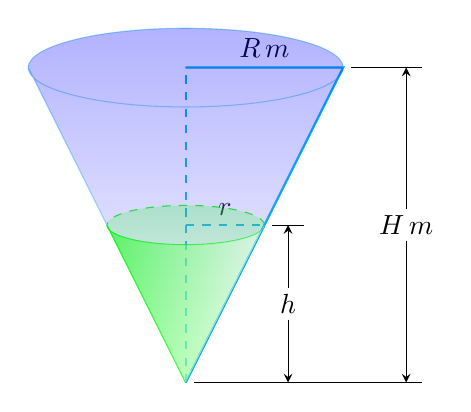
\begin{tikzpicture}[>=stealth]
\draw(0,0,0)--(2,4,0)--(0,4,0);
\draw[white](0,0,0)--(-2,4,0);
\draw[cyan!40](0,4,0)ellipse[x radius=2cm,y radius=0.5cm];
\draw[green,dashed](1,2)arc(0:180:1cm and 0.25cm);
\draw[green](-1,2)arc(180:360:1cm and 0.25cm);
\draw[green](0,0)--(-1,2);
\draw[cyan!40](-1,2)--(-2,4);
\draw[thick,cyan](0,0,0)--(2,4,0)--(0,4,0);
\draw[thick,cyan,dashed](0,0,0)--(0,4,0)
(0,2)--(1,2);
\draw(1,4)node[above]{$R\,m$}
(2.8,2)node[]{$ H\, m$}
(0.5,2)node[above]{$r$}
(1.3,1)node[]{$h$};
\draw(0.1,0)--(3,0)
(2.1,4)--(3,4)
(1.1,2)--(1.5,2);
\draw[->](2.8,1.8)--(2.8,0);
\draw[->](2.8,2.2)--(2.8,4);
\draw[->](1.3,0.8)--(1.3,0);
\draw[->](1.3,1.2)--(1.3,2);
\shade[top color=blue,opacity=0.3](0,4,0)ellipse[x radius = 2cm, y radius = 0.5cm]--(-2,4,0)--(0,0,0)--(2,4,0)--cycle;
\shade[top color=green,opacity=0.2](1,2)arc(0:180:1cm and 0.25cm)--(-1,2)--(0,0)--(1,2)--cycle;
\shade[left color=green,opacity=0.5](-1,2)arc(180:360:1cm and 0.25cm)--(1,2)--(0,0)--(-1,2)--cycle;
\end{tikzpicture}
\end{figure}
}
\end{center}
\vspace{0.5cm}



\vfill
\begin{center}
\line(1,0){300}\\
\end{center}
\centering
\vspace{0.1cm}
by: Nephat Jeshurun Mwanza
\end{titlepage}


\tableofcontents
\thispagestyle{empty}
\clearpage




\setcounter{page}{1}


\section{SETS}
$\bullet$ If $A$ is a set  and $x$ an element, we shall write $x\in A$ to mean that $x$ belongs to $A$.\\
$\bullet$ $x\not\in A$ means that $x$ is not a member of $A$.\\

\textbf{Example}\\ Let $A=\{2,4,6,8,10\}$. Then $4\in A$ but $5\not\in A$.\\


\textbf{Definition}:\\ If $A$ and $B$ are two sets we say that $A$ is a subset of $B$ written $A\subset B$ if for every\\ $x\in A\implies x\in B$.\\

\textbf{Definition}:\\ Two sets $A$ and $B$ are equal if both inclusions $A\subset B$ and $B\subset A$ hold.\\
$\bullet$ The empty set or null set is the set with no elements, denoted by $\emptyset$.\\
$*$  Note that $\emptyset$ is a subset of every set.\\
$\bullet$ The universal set is the set which contains all the elements under discussion, denoted by the letter $E$ or $\bigcup$.\\


\textbf{Example}\\ Let $\cup =\{1,2,3,4,5,6,7\}$ and $A=\{3,4,5,7\}$\\ Then the elements 1, 2, 5 which are in $\cup$  are not in $A$. The elements are said to be in the complement of $A$ written $A'$. That is $A'=\{1,2,5\}$.\\

\textbf{Definition}:\\ Let $A$ and $B$ be two sets. Then the difference $B-A$ is defined by $B-A=\{x:x\in B$ and $x\not\in A\}$\\

\textbf{Example}\\ Let $A=\{2,3,4,5,6,7,8\}$ and $B=\{0,1,2,3,4,5\}$. Then, $B-A=\{0,1\}$.\\
$*$ Note that  if $\cup$ is a universal set and $A$ is a set. Then the complement of $A$ can be written as $A'=\cup - A$.\\\\

\textbf{Universal Set}
\begin{enumerate}
\item[$\bullet$] If $E$ is the universal set and $A$ is a set then we can represent them diagramatically as
\end{enumerate}
% FIRST DIAGRAM

\begin{figure}[H]
\centering
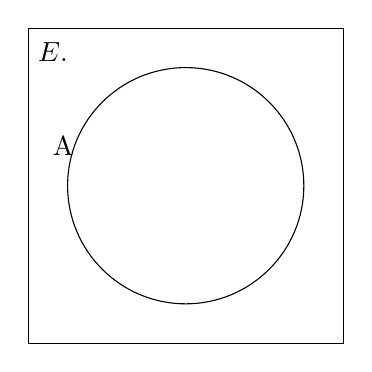
\begin{tikzpicture}
\draw(0,0) circle [radius=1.5cm]
(-1.3,0.5) node [text=black,left] {$\text{A}$};
\draw (-2,-2) rectangle (2,2)
(-2,1.7) node [text=black, right] {$E.$};
\end{tikzpicture}
\end{figure}









\pagebreak 
\subsection{Set Operation}
\textbf{Definition:}\\
Let $A$ and $B$ be two sets. Then the intersection of $A$ and $B$ is defined to be $$A\cap B =\{x:x\in A \hspace{0.3cm} \text{and}\hspace{0.3cm} x\in B\}$$


% SECOND DIAGRAM

\begin{figure}[H]
\centering
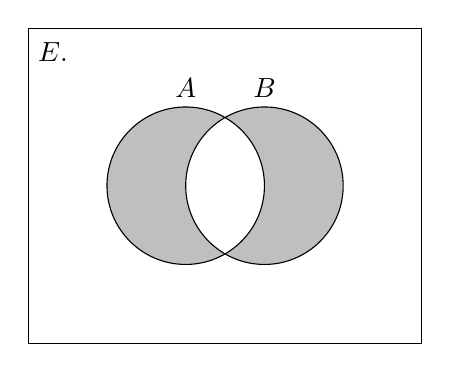
\begin{tikzpicture}[fill=lightgray]
\scope
\clip
(-2,-2)rectangle(2,2)
(1,0)circle(1);
\fill
(0,0)circle(1);
\endscope

\scope
\clip
(-2,-2)rectangle(2,2)
(0,0)circle(1);
\fill
(1,0)circle(1);
\endscope

\draw (0,0)circle(1)
(0,1)node[text=black, above]{$A$}
(1,0)circle(1)
(1,1)node[text=black, above]{$B$}
(-2,1.7)node[text=black, right]{$E.$};
\draw(-2,-2)rectangle(3,2);
\end{tikzpicture}
\end{figure}




$\bullet$ Two sets $A$ and $B$ are disjoint if $A\cap B=\emptyset$\\\\

\textbf{Definition}\\
Let $A$ and $B$ be two sets. Then the union of $A$ and $B$ is defined to be $$A\cup B=\{x:x\in A\hspace{0.2cm} \text{or}\hspace{0.2cm} x\in B\}$$


% THIRD DIAGRAM

\begin{figure}[H]
\centering
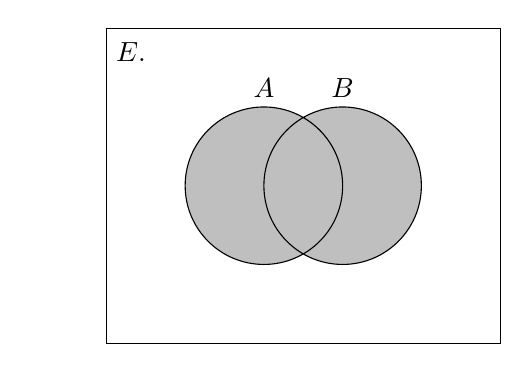
\begin{tikzpicture}[fill=lightgray]
\scope
\clip
(-2,-2)rectangle(2,2)
(2,0)circle(1);
\fill
(0,0)circle(1);
\endscope

\scope
\clip
(-2,-2)rectangle(2,2)
(-2,0)circle(1);
\fill
(1,0)circle(1);
\endscope

\draw (0,0) circle(1)
(0,1)node[text=black,above]{$A$}
(1,0)circle(1)
(1,1)node[text=black,above]{$B$}
(-2,1.7)node[text=black, right]{$E.$};

\draw(-2,-2)rectangle(3,2);
\end{tikzpicture}
\end{figure}








\textbf{Example}\\
Let
\begin{enumerate}
\item[ ] $A=\{1,2,3,4,5,6,7, 8\}$
\item[] $B=\{3,6, 9, 12, 15\}$
\item[] $C=\{2,5,7\}$
\end{enumerate}

Find the following:
\begin{enumerate}
\item $A\cap B$
\item $B\cup C$
\item $B\cap C$
\item $C-A$
\item $(A-B)\cup (B-A)$\\\\
\end{enumerate}


\textbf{Solution}
\begin{enumerate}
\item $A\cap B = \{3,6\}$
\item $B\cup C =\{2,3,5,6,7,9,12,15\}$
\item $B\cap C =\emptyset$
\item $C-A =\emptyset$
\item $(A-B)\cup (B-A)=\{1,2,4,5,7,8,9,12,15\}$\\\\
\end{enumerate}

$\bullet$ If $A\subset B$ then $B'\subset A'$
% DIAGRAM FOUR




\begin{figure}[H]
\centering
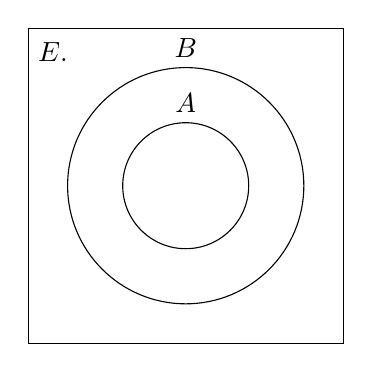
\begin{tikzpicture}
\draw (-2,-2)rectangle(2,2);
\draw(0,0)circle(1.5);
\draw(0,0)circle(0.8)
(0,0.8)node[above]{$A$}
(0,1.5)node[above]{$B$}
(-2,1.7)node[right]{$E.$};
\end{tikzpicture}
\hspace{0.5cm} $A\subset B\implies B'\subset A'$
\end{figure}







\vspace{1cm}
\subsection{Properties:}
\begin{enumerate}
\item Commutativity\\ for any sets $A$ and $B$
\begin{enumerate}
\item. $A\cup B=B\cup A$
\item. $A\cap B =B\cap A$
\end{enumerate}

\item Associativity\\ for any sets $A,B$ and $C$
\begin{enumerate}
\item. $A\cup (B\cup C ) = (A\cup B)\cup C$
\item. $A\cap (B\cap C) = (A\cap B)\cap C$
\end{enumerate}

\item Distributive Property\\ for any sets $A, B$ and $C$
\begin{enumerate}
\item. $A\cap (B\cup C) = (A\cap B) \cup (A\cap C)$
\item. $A\cup (B\cap C) = (A\cup B)\cap (A\cup C)$
\end{enumerate}





\pagebreak
\item De Morgan's Law\\ for any sets $A$ and $B$
\begin{enumerate}
\item. $(A\cup B)'=A'\cap B'$
\item. $(A\cap B)' = A'\cup B'$
\end{enumerate}

\item Let $\bigcup$ be the  universal set and $A$ be any set, then
\begin{enumerate}
\item. $A\cup A'=\bigcup$
\item. $A\cap A' = \emptyset$
\item. $\emptyset \cup \bigcup = \bigcup$
\item. $\emptyset \cap \bigcup =\emptyset$\\
\end{enumerate}

\item If $A\subset B$, then
\begin{enumerate}
\item. $A\cap B=A$
\item. $A\cup B=B$\\
\end{enumerate}

\item[$\bullet$] Note that $A''=A$\\
\end{enumerate}


\textbf{Examples:}\\ Simplify
\begin{enumerate}
\item $(x\cup y)\cap (x\cup y')$
\item $[(x\cap y)'\cap x]'$\\
\end{enumerate}



\textbf{Solution}
\begin{enumerate}
\item[] \hspace{0.2cm}
$
\begin{matrix}
(x\cup y)\cap (x\cup y') & = & x\cup (y\cap y')\\
                         & = & x \cup \emptyset\\
                         & =& x\\
\end{matrix}
$\\\\\\

\item[]
$
\begin{matrix}
[(x\cap y)'\cap x]' & = & (x\cap y)'' \cup x'\\\\
                    & = & (x\cap y) \cup x'\\\\
                    & = & (x\cup x')\cap (y\cup x')\\\\
                    & = & \bigcup \cap (y\cup x')\\\\
                    & = & y\cup x'\\
\end{matrix}
$\\\\\\
\end{enumerate}


\textbf{Example:}\\
Prove that $(A\cap B)' =A'\cup B'$\\\\

\textbf{Proof}:\\
We must show that $(A\cap B)'\subset A'\cup B'$ and also that $A'\cup B'\subset (A\cap B)'$.\\

\textbf{case I:}\\
To show that $(A\cap B)'\subset A'\cup B'$.\\
Let $x\in (A\cap B)'$, the we must show that $x\in A'\cup B'$.\\
Now, if $x\in (A\cap B)'$ then $x\not\in (A\cap B)$\\
$\implies \hspace{0.5cm} x\not\in A$ and $x\not\in B$\\
$\implies \hspace{0.5cm} x\in A'$ or $x\in B'$\\
$\implies \hspace{0.5cm} x\in A'\cup B'$\\
Therefore $(A\cap B)'\subset A'\cup B'\hspace{0.3cm} \cdots\cdots\cdots\hspace{0.3cm} (1)$\\
Since every element in $(A\cap B)'$ is also in $A'\cup B'$.\\

\textbf{case II}\\
To show that $A'\cup B' \subset (A\cap B)'$\\
Conversely, if $x\in A'\cup B'$ then\\
$\implies \hspace{0.5cm} x\in A'$ or $x\in B'$\\
$\implies \hspace{0.5cm} x\not\in A$ and $x\not\in B$\\
$\implies \hspace{0.5cm} x\not\in (A\cap B)$\\
$\implies \hspace{0.5cm} x\in (A\cap B)'$\\
Hence $A'\cup B'\subset (A\cap B)'\hspace{0.3cm} \cdots\cdots\cdots \hspace{0.2cm} (2)$\\

Since $(A\cap B)'\subset A'\cup B'$ and $A'\cup B'\subset (A\cap B)'$. Thus $(A\cap B)' =A' \cup B'$.\\\\



\textbf{Example:}\\
Let $A, B$ and $C$ be any sets. Prove that $A\cap (B\cup C)=(A\cap B)\cup (A\cap C)$.\\\\




\textbf{Example}
\begin{enumerate}
\item[] $\bigcup = \{1,2,3,4,5,\cdots\cdots\cdots, 10\}$
\item[] $A = \{1,2,3,4,5\}$
\item[] $B = \{2,3,5,7\}$
\item[] $C = \{3,4,5,6,7,8\}$\\\
\end{enumerate}

Verify the following: $(A\cup B)' = A'\cap B'$
\begin{enumerate}
\item[] $A\cup B = \{1,2,3,4,5,7\}$
\item[] $(A\cup B)' = \{6,8,9,10\}$
\item[] $A' =\{6,7,8,9,10\}$
\item[] $B' = \{1,4, 6, 8, 9, 10\}$
\item[] $A'\cap B' = \{6, 8, 9, 10\}$\\
\end{enumerate}
Thus, $(A\cup B)' =\{6,8,9,10\}=A'\cap B'$\\\\




\pagebreak
$\bullet$ Let $\bigcup$ be a universal set and let $A$ and $B$ be sets. Prove that 
\begin{enumerate}
\item $\bigcup - A=A'$
\item $A-B=A\cap B'$
\item $A-B\subset A$\\\\
\end{enumerate}












\pagebreak
% SETS OF NUMBERS
\section{SETS OF NUMBERS}
\begin{enumerate}
\item[$\bullet$] Natural numbers, $\mathbb{N}=\{0,1,2,3,4,\cdots\cdots\cdots \}$
\item[$\bullet$] Integers, $\mathbb{Z}=\{0,\pm 1, \pm 2, \pm 3,\cdots\cdots\cdots \}$
\item[$\bullet$] Positive integers, $\mathbb{Z}^+=\{+1, +2, +3, \cdots\cdots\cdots \}$
\item[$\bullet$] $\mathbb{Q}$ set of rational numbers.
\item[$\bullet$] $\mathbb{R}$ set of real numbers.
\item[$\bullet$] $\mathbb{C}$ the set of complex numbers.
\item[$\bullet$] Prime numbers, $\{2, 3, 5, 7, 11, 13,\cdots\cdots\cdots \}$
\item[$\bullet$] Odd numbers, $\{ ,3 , 5, 7, 9, 11, 13, 15, \cdots\cdots\cdots \}$
\item[$\bullet$] Even numbers, $\{ , 2, 4, 6, 8, 10, \cdots\cdots\cdots \}$\\
\end{enumerate}




\subsection{Rational Numbers}
\begin{enumerate}
\item[$\bullet$] The set of rational numbers denoted by $\mathbb{Q}$ is defined $\mathbb{Q}=\bigg\{\dfrac{a}{b}:a,b\in \mathbb{Z}$ and $b\neq 0\bigg\}$.
\item[$\bullet$] The decimal representation of any rational decimal e.g $\dfrac{4}{25}=0.16$ or it is a repeating decimal e.g  $\dfrac{5}{7}=0.71428571429$
\item[$\bullet$] When a rational number is expressed in decimal form we can find integers $a$ and $b$ such that the number is in the form $\dfrac{a}{b}$.
\item[$\bullet$] Note that when a decimal is repeating we put a bar over a repeating decimal\\ e.g \hspace{0.2cm}$\dfrac{5}{7}=0.\overline{714285}$\\
\end{enumerate}


\textbf{Examples}
\begin{enumerate}
\item Show that $0.354\overline{54}$ is a rational number.\\

\textbf{Solution}\\\\
Let  $x=0.354\overline{54}$ then\\\\   $
\begin{matrix}
 x & = & 0.354\overline{54}\cdots\cdots\cdots (\text{i})\\
                      10x & = & 3.54\overline{54}\cdots\cdots\cdots (\text{ii})\\
                      100x & = & 35.4\overline{54}\cdots\cdots\cdots (\text{iii})\\
                      1000x & = & 354.\overline{54}\cdots\cdots\cdots (\text{iv})\\
                      
\end{matrix}
$\\\\

Subtract (ii) from (iv)\\\\
$
\begin{matrix}
1000x & = & 354.\overline{54}\\
\underline{-10x} & = & \underline{- 3.5454}\\
990x & = & 351\\
\end{matrix}                      
 $ \\
 
$\implies \hspace{1cm} 990x=351\hspace{1cm}\implies \hspace{1cm} x=\dfrac{351}{990}=\dfrac{39}{110}$\\\\ 
$\therefore \hspace{0.5cm} x=\dfrac{39}{110}$\\\\



\item Express $3.8\overline{3}$ in the form $\dfrac{a}{b}$ where $a$ and $b$ are integers.\\\\

\textbf{Solution}\\
Note that $3.8\overline{3} = 3.83333$\\\\
Let $x=3.8333$ then\\

$
\begin{matrix}
10x & = 38.3333\\
100x & = 383.33\\
\end{matrix} 
$\\\\  

$\implies
\begin{matrix}
100x & = & 383.33\\
\underline{-10x} & = & \underline{38.33}\\
90x & = & 345\\
\end{matrix}
$\\\\

$90x=345\hspace{0.7cm} \implies \hspace{0.7cm} x=\dfrac{345}{90}=\dfrac{23}{6}$\\\\

$\therefore \hspace{0.7cm} x=\dfrac{23}{6}$\\\\

\item Show that $0.217\overline{217}$ is a rational number.\\\\
\textbf{Solution}\\\\
Let $x=0.217\overline{217}$\\\\
Multiply by $1 000$ both sides, we get $1 000x = 217.217$ then\\

$
\begin{matrix}
1 000x & = & 217.217\\
\underline{-x} & = & \underline{-0.217}\\
999x & = & 217\\
\end{matrix} 
$\\\\

$999x=217\hspace{0.7cm} \implies \hspace{0.7cm} x=\dfrac{217}{999}$\\\\


\item Express $4.75$ in the form $\dfrac{a}{b}$ when $a$ and $b$ are integers.\\\\

\pagebreak
\textbf{Solution}\\
Let $x=4.75$, multiply by 100 both sides, we get $100x=475$\\\\   
$\implies \hspace{0.7cm} x=\dfrac{475}{100}\hspace{0.7cm} \implies \hspace{0.7cm} x=\dfrac{19}{4}$.\\\\

\item Express $-0.72\overline{72}$ in the form $\dfrac{a}{b}$.\\\\
\textbf{Solution}\\\\
$
\begin{matrix}
\text{Let}\hspace{0.7cm} x &= &-0.72\overline{72}\\
100x & = & -72.72\\
\end{matrix} 
$ \\\\


$
\begin{matrix}
100x & = & -72.72\\
\underline{-x} & = & \underline{+ 0.72}\\
99x & = & -72\\
\end{matrix}
$ \\\\

$\implies \hspace{1cm} x=\dfrac{-72}{99}$\\\\      
\end{enumerate}




\subsection{Irrational Numbers}
\begin{enumerate}
\item[$\bullet$] An irrational number is a number which cannot be expressed in the form $\dfrac{a}{b}$ for some integers $a$ and $b$.
\item[$\bullet$] Decimal representation of an irrational number non terminating and non repeating.
\item[$\bullet$] To show that there are numbers which are not rational.\\
Note that: if $P$ is an integer such that $P^2$ is divisible by 2 then $P$ itself is divisible by 2.\\

\textbf{Proof:}\\
Every integer can be expressed in the form\\\\
$P =
\begin{cases}
2m\\
2m+1\\
\end{cases}
$ where $m$ is an integer.\\\\
Then\\\\
$P^2=
\begin{cases}
4m^2\\
4m^2+4m+1\\
\end{cases}
$\\\\

But $P^2$ is divisible by 2, therefore $P^2$ must be of the form $P^2=4m^2$.\\ This implies that $P=2m$ which is also divisible by 2.\\\\

\item[$\bullet$] Prove that $\sqrt{2}$ is not a rational number.\\ To prove that $\sqrt{2}$ is not rational, we prove by contradiction by assuming $\sqrt{2}$ is rational.\\

\textbf{Proof:}\\
Suppose that to the contrary $\sqrt{2}$ is rational. Then there are integers $m$ and $n$ such that $\sqrt{2}=\dfrac{m}{n},$ where $\dfrac{m}{n}$ is a fraction in its lowest terms.\\ Now square both sides\\\\ $2=\dfrac{m^2}{n^2}\hspace{0.7cm} \implies \hspace{0.7cm} 2n^2=m^2$\\\\
This shows that $m^2$ is a multiple of 2 and so $m^2$ is divisible by 2.\\
Since $m^2$ is divisible by 2 then $m$ itself is divisible by 2. Thus $m$ can be written in the form $m=2k$ for some integer $k$. Thus, from $2n^2=m^2$, we get $$2n^2=(2k)^2\hspace{0.7cm} \implies \hspace{0.7cm} 2n^2=4k^2$$
Thus $n^2$ is divisible by 2 implying that $n$ itself is divisible by 2.\\
Thus $m$ and $n$ have a common factor 2 which is a contradiction to our assumption that they have no common factor.\\ We therefore conclude that $\sqrt{2}$ is not a rational number.\\
\end{enumerate}


\textbf{Example:}\\
Show that $2+\sqrt{3}$ is not a rational number.\\

\textbf{Proof}\\
Suppose that $2+\sqrt{3}$ is a rational number. Then by definition there are integers $a$ and $b$ with $b\neq 0$ such that $2+\sqrt{3}=\dfrac{a}{b}$.$$\implies \hspace{0.7cm} \sqrt{3}=\frac{a}{b}-2\hspace{0.7cm} \implies \hspace{0.7cm}\sqrt{3}=\frac{a-2b}{b}$$
Since $a$ and $2b$ are integers then $a-2b$ is also an integer, say $m$. Thus $\sqrt{3}=\dfrac{m}{b}$ where $m$ and $b$ are integers.\\
But LHS is irrational since $\sqrt{3}$ is irrational while the RHS is rational. This is a contradiction since there is no irrational number which is also rational.
Therefore our assumption that $2+\sqrt{3}$ is rational is false.\\ Hence $2+\sqrt{3}$ is an irrational number.\\\\



\subsection{Real Numbers}
The union of the set of rational numbers with the set of irrational numbers is the set of real numbers denoted by $\mathbb{R}$.\\
To represents the subset of the set of real numbers we either use blackest. \\e.g\hspace{0.3cm} $(\cdot,\cdot),\hspace{0.5cm} (\cdot,\cdot],\hspace{0.5cm}[\cdot,\cdot),\hspace{0.5cm} [\cdot,\cdot]$\\\\
$($ or $)$ the number not included.\\
$[$ or $]$ or $\{$ or $\}$ number included.\\\\






\pagebreak
\textbf{Example:}
\begin{enumerate}
\item[$\bullet$] $[-2,0)$. This means $-2$ is part of the set while 0 is not part of the set.
\item[$\bullet$] Set builder notation can also be used to describe the set $$[-2,0)=\{x\in \mathbb{R}:-2\leq x<0\}$$
\item[$\bullet$] When using interval notation the smaller number must be on the left while the bigger one must be on right side.
\item[$\bullet$] $\infty$ infinity is not a real number.\\ The blacket must always be open because it is not a real number.\\\\
\end{enumerate}


\textbf{Operation On $\mathbb{R}$}\\

\textbf{Example}\\
Let $A=\{x\in \mathbb{R}:-7\leq x<3\}$ and $B=\{x\in \mathbb{R}:x\geq -1\}$\\

Find
\begin{enumerate}
\item $A\cap B$
\item $A'$\\
\end{enumerate}

\textbf{Solution}
\begin{enumerate}
\item $A=[-7,3),\hspace{0.7cm} B=[-1,8)\hspace{0.7cm} \implies \hspace{0.7cm} A\cap B=[-1,3)$

\item $A'=(-\infty, -7)\cup [3,\infty )$\\\\
\end{enumerate}

\textbf{Example}\\
$\cup =(-7,10]$ be the universal set and let $A=[-3,7],\hspace{0.3cm} B=(-2,5)$ and $C=(-6,10]$\\\\

Find
\begin{enumerate}
\item $A\cap B$
\item $\cup -C$\\\
\end{enumerate}

\textbf{Solution}
\begin{enumerate}
\item $A\cap B=(-2,5)$
\item $\cup - C = $ note $-7$ is $\not\in \cup$ so it cannot be in $C'$, thus $C'=(-7,-6]$\\\\
\end{enumerate}








\pagebreak
\textbf{Properties Of $\mathbb{R}$}\\
Real numbers have certain properties which allow us to compare any two real numbers or to perform some algebraic computation.

\begin{enumerate}
\item \textbf{Algebraic Properties}\\
If $x$, $y$ and $z$ are any three numbers, then
\begin{enumerate}
\item $x+y=y+x$ \hspace{0.4cm} Commutative law

\item $
\begin{matrix}
x+(y+z) & = & (x+y)+z\\
x(yz) & = & (xy)z\\
\end{matrix}
$\hspace{0.4cm} Associative Law\\

\item $x+0=0+x=x,\hspace{0.4cm}$ 0 is addictive identity

\item $x\cdot 1=1\cdot x=x,\hspace{0.4cm}$ 1 is multiplicative identity

\item $x+(-x)=x-x=-x+x=0$

\item $x(y+z)=xy+xz$,\hspace{0.4cm} Distributive Law\\\\
\end{enumerate}

\item \textbf{Order Relations:}\\
If $x$ and $y$ are any two real numbers then
\begin{enumerate}
\item $x$ is greater than $y$ written $x>y$ if $x-y>0.$

\item $x$ is less than $y$ written $x<y$ if $x-y<0$.

\item $x$ is equal to $y$ written $x=y$ if $x-y=0$.\\\\
\end{enumerate}


\item \textbf{Absolute Value:}\\
\textbf{Definition:} An absolute value denoted by $|\cdot|$
$$|x|=
\begin{cases}
x, & \text{if}\hspace{0.3cm} x\geq\\
-x, & \text{if} \hspace{0.3cm} x<0\\
\end{cases}
$$

The absolute of a real number is always positive.\\
e.g
\begin{enumerate}
\item[(a).] $|8|=8$
\item[(b).] $|-23|=-(-23)$\\
\end{enumerate}
\end{enumerate}


\textbf{Example}\\
Find the value of $|a-b|$ when
\begin{enumerate}
\item[(i).] $a=7,\hspace{0.4cm} b=4$
\item[(ii).] $a=-6,\hspace{0.4cm} b=8$
\item[(iii).] $a=2,\hspace{0.4cm} b=11$\\\\
\end{enumerate}



\textbf{Example:}\\
Given that $a<b$. Express $P$ in terms of $a$ and $b$, if $\dfrac{|P-a|}{|b-a|}=\dfrac{3}{4}$.\\\\

\textbf{Solution}\\\\
$\dfrac{|P-a|}{|b-a|}=\dfrac{3}{4}\hspace{0.7cm} \implies \hspace{0.7cm} \dfrac{|P-a|}{b-a}=\dfrac{3}{4}$\\\\

$\implies \hspace{0.7cm} |P-a|=\dfrac{3}{4}(b-a)$\\\\

$\implies \hspace{0.7cm} |P-a|=\dfrac{3}{4}b-\dfrac{3}{4}a$\\\\

\textbf{case I}: if $P\geq a$ then $P-a\geq 0$
\begin{align*}
\implies \hspace{0.7cm} P-a & = \frac{3b}{4}-\frac{3a}{4}\hspace{0.7cm} \implies \hspace{0.7cm}
                        P  = \frac{3b}{4}-\frac{3a}{4}+a\\\\
                          & = \frac{3b}{4}+\frac{-3a+4a}{4}\\\\
\implies \hspace{0.7cm} P & = \frac{3b}{4}+\frac{a}{4}\\\\
\end{align*}


\textbf{Case II:} If $P<a$ then $P-a<0$.\\
Therefore, $|P-a|=-(P-a)=-P+a$ in this case
\begin{align*}
-P+a & = \frac{3b}{4}-\frac{3a}{4}\hspace{0.7cm} \implies \hspace{0.7cm} -P=\frac{3b}{3}-\frac{3a}{4}-a\\\\
- P & = \frac{3b}{4}-\frac{7a}{4}\\\\
\implies \hspace{0.7cm} P & = \frac{7a}{4}-\frac{3b}{4}\\\\
\end{align*}



\textbf{Example}\\
Solve the equation, $|x-7|=11$.\\\\

\textbf{case I:}
$x>7$ so that $x-7=0$\\ in this case $|x-7|=x-7=11\hspace{0.5cm}$
$\implies \hspace{0.5cm} x=7+11=18$\\\\

\textbf{case II:} $x<7$, so that $|x-7|=-(x-7)$\\
In this case $|x-7|=-(x-7)=11$\\
$x-7=-11\hspace{0.5cm} \implies \hspace{0.5cm} x=-11+7=-4$\\\\

\begin{enumerate}
\item[$\bullet$] Let $k$ be a positive real number consider the inequality $|x|<k$.\\
If $x\geq 0$ then $|x|=x$ so that $|x|<k\hspace{0.4cm} \implies \hspace{0.4cm} x<k\hspace{0.2cm} \cdots\cdots\cdots\hspace{0.2cm}(1)$\\ \\ 
If $x<0$ then $|x|=-x$ so that $|x|<k\hspace{0.5cm} \implies \hspace{0.5cm} -x<k\hspace{0.4cm}\\ \implies \hspace{0.4cm} -k<x\hspace{0.2cm} \cdots\cdots\cdots \hspace{0.2cm} (2)$\\
Now, combining the two inequalities we conclude that $|x|<k \iff -k<x<k$.\\\\
\end{enumerate}















\pagebreak
% COMPLEX NUMBERS
\section{COMPLEX NUMBERS}
Define $i=\sqrt{-1}$. Then $i^2=-1$\\\\
e.g $\sqrt{-25}=\sqrt{-1}\cdot \sqrt{25}=i\cdot 5=5i$\\\\
If $b$ is a real number the numbers of the for $bi$ are called imaginary numbers e.g $5i$, $-12i$, $17i$, $-102i$ are examples of imaginary numbers.\\
If $a$ and $b$ are real numbers the number of the form $a+bi$ is called a complex number e.g $3+2i$, $7-23i$, $-14+35i$ e.t.c\\\\
The set of all complex numbers is denoted by $\mathbb{C}$\\
% DIAGRAM 1

\begin{figure}[H]
\centering
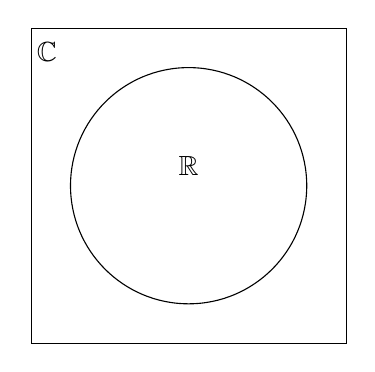
\begin{tikzpicture}
\draw(0,0) circle [radius=1.5cm]
(0,0) node [text=black, above] {$\mathbb{R}$};
\draw(-2,-2) rectangle (2,2)
(-1.8,1.95) node [text=black, below] {$\mathbb{C}$};
\end{tikzpicture}
\end{figure}





Let $z=x+iy$ be a complex number. Then $x$ is called the real part of $z$, $y$ is called the imaginary part of $z$.\\\\
Re$z=x$ to mean the real part of $z$ is $x$.\\

Im$z=y$  to mean the imaginary part $z$ is $y$.\\\\

Let $z_1=x_1+iy_1$ and $z_2=x_2+iy_2$ be two complex numbers. Then
\begin{enumerate}
\item $z_1=z_2$ if and only if $x_1=x_2$ and $y_1=y_2$.

\item $z_1\pm z_2 = (x_1\pm x_2)+i(y_1\pm y_2)$\\
\end{enumerate}

e.g $(4+3i)+(7-5i)=(4+7)+i(3-5)=11-2i$\\\\

\textbf{Example:}\\
Find $x$ and $y$ such that
\begin{enumerate}
\item $x+iy=7-4i$

\item $(3x-iy)+(2+13i)=-7+3i$\\
\end{enumerate}

\textbf{Solution}
\begin{enumerate}
\item $x+iy=7-4i$ \\
Equating the real parts and the imaginary parts, we get $x=7$, $y=-4$.

\item $(3x-iy)+(2+13i) =-7+3i$\\
Adding the real parts and the imaginary parts\\
$(3x-iy)=-9-10i$\\
$\implies \hspace{0.4cm} 3x=-9$ and $-y=-10$\\
$\implies \hspace{0.4cm} x=-3$ and $y=10$\\
\end{enumerate}


\textbf{Product}\\
Let $z_1=x_1+iy_1$ and $z_2=x_2+iy_2$ be two complex numbers.\\ Then $z_1z_2=(x_1x_2-y_1y_2)+i(x_1y_2+x_2y_1)$\\\\

\textbf{Examples:}\\
Find
\begin{enumerate}
\item[(a).] $(3+2i)(4-5i)$
\item[(b).] $(3+\sqrt{2}i)(3-\sqrt{2}i)$\\
\end{enumerate}


\textbf{Solution}
\begin{align*}
(3+2i)(4-5i) &= (3\times 4-(-5\times 2))+i(3(-5)+4(2))\\
             &= (12+10)+i(-15+8)\\
             &= 22-7i\\
\end{align*}



\textbf{Definition}\\
Let $z=x+iy$ be a complex number, then the modulus of $z$ denoted by $|z|$ is defined to be $|z|=\sqrt{x^2+y^2}$.\\\\

\textbf{Example}\\
Find the modulus of each of the following complex number
\begin{enumerate}
\item[(a).] $5+12i$
\item[(b).] $-8+6i$
\item[(c).] $15i$
\item[(d).] $(1-\sqrt{2})+(\sqrt{2}+2)i$\\

\item[$\bullet$] Note that $15i=0+15i$\\
\end{enumerate}


\textbf{Solution}\\
$z=x+iy$, $|z|=\sqrt{x^2+y^2}$\\

$\implies \hspace{0.3cm} |z|=\sqrt{5^2+(12)^2}=\sqrt{25+144}=\sqrt{169}=13$\\\\


\textbf{Definition:}\\
Let $z=x+iy$ be a complex number, then the conjugate of $z$ denoted by $\overline{z}$ is defined to be $\overline{z}=x-iy$. Thus the conjugate of a complex number is obtained by changing the sign of the imaginary part.\\\\
e.g $z=7+13i$ then $\overline{z}=7-13i$\\\\

$\bullet$ Note also that if $z=x+iy$ then $z\overline{z}=(x+iy)(x-iy)=x^2+y^2=|z|^2$\\\\

\textbf{Definition}:\\
Let $z_1=x_1+iy_1$ and $z_2=x_2+iy_2$ be two complex numbers. Then $\dfrac{z_1}{z_2}=\dfrac{z_1\overline{z_2}}{z_2\overline{z_2}}$ that is
\begin{align*}
\frac{x_1+iy_1}{x_2+iy_2} & =\frac{(x_1+iy_1)(x_2-iy_2)}{(x_2+iy_2)(x_2-iy_2)}\\\\
                          & = \frac{x_1x_2+y_1y_2+i(x_2y_1-x_1y_2)}{x_2^2+y_2^2}\\\\
                          & = \frac{x_1x_2+y_1y_2}{x_2^2+y^2_2}+\frac{x_2y_1-x_1y_2}{x^2_2+y^2_2}\\
\end{align*}



\textbf{Example}
\begin{align*}
\frac{2+i}{3-2i} & = \frac{(2+i)(3+2i)}{(3-2i)(3+2i)} = \frac{(6-2)+i(4+3)}{3^2+2^2}\\\\
                 & = \frac{4+7i}{13}\\\\
                 & = \frac{4}{13}+\frac{7}{13}i\\
\end{align*}



\textbf{Example}\\
Express each of the following complex numbers in the form $a+ib$ where $a$ and $b$ are real numbers. Hence find $|z|$ in each  case.
\begin{enumerate}
\item[]
\begin{enumerate}
     \item $(4+i)^2$
     \item $\dfrac{2-5i}{3+2i}$\\
     \item $\dfrac{3+5i}{4-3i}$
\end{enumerate}
\end{enumerate}




\textbf{Solutions}
\begin{align*}
z & = (4+i)^2=(4+i)(4+i)\\
  & = (16-1)+8i\\
\implies \hspace{0.5cm} & = 15+8i\\\\
\therefore \hspace{0.5cm} |z| & = \sqrt{(15)^2+(8)^2}=\sqrt{289}=17\\\\
\end{align*}


\begin{align*}
z & = \frac{2-5i}{3+2i}=\frac{2-5i}{3+2i}\times \frac{3-2i}{3-2i}\\\\
  & = \frac{(6-10)-i(15+4)}{9+4}=\frac{-4-19i}{13}\\\\
\implies \hspace{0.5cm} z & = \frac{-4}{13}-\frac{19}{13}i\\\\
\therefore \hspace{0.5cm} |z| & = \sqrt{\bigg(\dfrac{-4}{13}\bigg)^2+\bigg(\dfrac{-19}{13}\bigg)^2}=\frac{1}{13}\sqrt{16+36}=\frac{\sqrt{377}}{13}\\\\
\end{align*}




\begin{align*}
z & = \frac{3+5i}{4-3i}=\frac{3+5i}{4-3i}\times \frac{4+3i}{4+3i}\\\\
  & = \frac{(12-15)+i(9+20)}{16+9}\\\\
\implies \hspace{0.5cm} z & = \frac{-3}{25}+\frac{29}{25}i\\\\
\therefore \hspace{0.5cm} |z| & = \sqrt{\bigg(\dfrac{-3}{25}\bigg)^2+\bigg(\dfrac{29}{25}\bigg)^2}=\frac{1}{25}\sqrt{9+841}=\frac{\sqrt{850}}{25}\\\\
\end{align*}













\pagebreak
% SURDS
\section{SURDS}
Numbers of the form $\sqrt{2}$, $\sqrt{3}$, $\sqrt{5}$, $\cdots \cdots$ are called surds.\\\\
Take note that e.g $\sqrt{2}$ can be written as $2^{\frac{1}{2}}$ so that
\begin{align*}
\sqrt{2}\cdot \sqrt{2} & = 2^{\frac{1}{2}}\times 2^{\frac{1}{2}}\\
& = 2^{\frac{1}{2}+\frac{1}{2}}\\
& = 2^1\\
& = 2\\
\end{align*}



\textbf{Example}\\\\
Express each of the following in its simplest possible surd.
\begin{enumerate}
\item $\sqrt{12}$\\
\item $\sqrt{63}$\\
\item $\sqrt{486}$\\\\
\end{enumerate}



\textbf{Solution}
\begin{enumerate}
\item $\sqrt{12}=\sqrt{4\times 3}=\sqrt{4}\times \sqrt{3}=2\sqrt{3}$\\
\item $\sqrt{63}=\sqrt{9\times 7}=\sqrt{9}\times \sqrt{7}=3\sqrt{7}$\\
\item $\sqrt{486}=\sqrt{81 \times 6}=\sqrt{81}\times \sqrt{6}=9\sqrt{6}$\\
\end{enumerate}

\textbf{Example}\\
In each of the following expand the given expression and simplify.
\begin{enumerate}
\item $(1+2\sqrt{5})(2+\sqrt{5})$\\
\item $(7-3\sqrt{7})(3+2\sqrt{7})$\\\\
\end{enumerate}

\textbf{Solution}
\begin{enumerate}
\item
\begin{align*}
(1+2\sqrt{5})(2+\sqrt{5}) &= 1(2+\sqrt{5})+2\sqrt{5}(2+\sqrt{5})\\
& = 2 + \sqrt{5}+4\sqrt{5}+2(5)\\
& = 2 + 10 +5\sqrt{5}\\
& = 12+5\sqrt{5}\\
\end{align*}

\item
\begin{align*}
(7-3\sqrt{7})(3+2\sqrt{7}) & = 7(3+2\sqrt{7})-3\sqrt{7}(3+2\sqrt{7})\\
& = 21 + 14\sqrt{7}-9\sqrt{7}-6(7)\\
& = 21-42+5\sqrt{7}\\
& = -21+5\sqrt{7}\\\\
\end{align*}
\end{enumerate}


When a rational contains a surd in the denominator we can simply by removing a surd from the denominator so that the denominator contains integers. You multiply both the numerator and denominator by the harmonic conjugate of the denominator, the process of removing a surd from the denominator is called rationalizing the denominator. For example to rationalize the denominator for $\dfrac{3}{\sqrt{7}}$, we find a number which we can multiply to get an integer $$\frac{3}{\sqrt{7}}=\frac{3}{\sqrt{7}} \times \frac{\sqrt{7}}{\sqrt{7}}=\frac{3\sqrt{7}}{7}$$\\

\textbf{Example}\\
Rationalize the denominator for $\dfrac{3}{5+\sqrt{7}}$\\
\begin{align*}
\frac{3}{5+\sqrt{7}} & =\frac{3}{5+\sqrt{7}}\times \frac{5-\sqrt{7}}{5-\sqrt{7}}\\\\
& = \frac{15-3\sqrt{7}}{25-7}\\\\
& =\frac{15}{18}-\frac{3\sqrt{7}}{18}\\\\
& = \frac{5}{6}-\frac{\sqrt{7}}{6}\\\\
\end{align*}


\textbf{Example}\\\\
Express $\dfrac{1-5\sqrt{2}}{2\sqrt{2}+5}$ in the form $a+b\sqrt{2}$ where $a$ and $b$ are rational numbers.\\
\begin{align*}
\frac{1-5\sqrt{2}}{2\sqrt{2}+5} & =\frac{(1-5\sqrt{2})(2\sqrt{2}-5)}{(2\sqrt{2}+5)(2\sqrt{2}-5)}\\\\
&=\frac{2\sqrt{2}-5-10(2)+25(\sqrt{2})}{4(2)-25}\\\\
&=\frac{-5-20+2\sqrt{2}+25\sqrt{2}}{8-25}\\\\
&=\frac{-25+27\sqrt{2}}{-17}\\\\
& =\frac{-25}{-17}+\frac{27}{-17}\\\\
& =\frac{25}{17}-\frac{27\sqrt{2}}{17}\\\\
\end{align*}















\pagebreak
%BINARY OPERATIONS
\section{BINARY OPERATIONS}
A binary operation is denoted by '$0$' or '$*$' on a non-empty set $G$ is a rule which associates to each pair of elements $a, b$ in $G$ a unique element $a*b$ of $G$.\\\\

\textbf{Examples}
\begin{enumerate}
\item Addition $(+)$ is a binary operation on a set of natural numbers $\mathbb{N}$, since if $m$ and $n$  are natural numbers then $m+n$ is also a natural number.\\
However, subtraction is not a binary operation on the set of natural numbers since $m-n$ may not be a natural number. e.g $6-9=-3$ and $-3$ is not a natural number.
\item Both addition and subtraction are binary operation on $\mathbb{Z}$ the  set of integers.\\ Whenever $*$ is binary of a set $G$ we say $G$ is closed under the operation $*$ or we say the closure property is satisfied in $G$ with respect to the operation $*$.\\
\end{enumerate}


\textbf{Example}\\ Let $X=\{-1,0,1\}$ be a set. Determine whether each of the following operations is binary on $X$ or not
\begin{enumerate}
\item[(a).] addition
\item[(b).] subtraction
\item[(c).] multiplication
\item[(d).] division\\
\end{enumerate}

\textbf{Solution:}
\begin{enumerate}
\item[(a).] Addition is Not. e.g $1+1=2\not\in X.$
\item[(b).] Subtraction is Not. e.g $-1-1=-2\not \in X$.
\item[(c).] Multiplication is binary on $X$.
\item[(d).] Division is Not, you cannot divide by zero.\\
\end{enumerate}





\pagebreak
\textbf{Example:}\\ Let the operation $*$ be defined by $a*b=2^{a^2+b}$ where $a,b \in \mathbb{R}$.
\begin{enumerate}
\item[(i).] Is the operation binary on $\mathbb{R}$
\item[(ii).] Evaluate $3*2$\\
\end{enumerate}


\textbf{Solution}\\ The operation is evidently binary, since if $a\in \mathbb{R}$ and $a^2\in \mathbb{R}$ and $b\in \mathbb{R}$ then $a^2+b\in \mathbb{R}$ which implies that $2^{a^2+b}\in \mathbb{R}.$\\\\ $3*2=2^{3^2+2}=2^{9+2}=2^{11}$\\



\textbf{Definition:}\\ The binary $*$ on $G$ is
\begin{enumerate}
\item[(i).] commutative if for every pair $a,b\in G$, \\ $a*b=b*a$
\item[(ii).] associative if for all $a,b,c\in G$,\\ $a*(b*c)=(a*b)*c$\\
\end{enumerate}


\textbf{Example:}\\ Let $G=\mathbb{Z}$ be the set of integers. Both addition and subtraction are binary on $\mathbb{Z}$.\\\\
\textbf{Question:}
\begin{enumerate}
                 \item[(1).] Are they both commutative?
                 \item[(2).] Are they both associative?\\
\end{enumerate}


\textbf{Solution}
\begin{enumerate}
\item Addition is both commutative and associative on $\mathbb{Z}$\\ e.g $-3+5=5+(-3)=2$
\item Subtraction is neither associative nor commutative, e.g $a*b=a-b$ on $\mathbb{Z}$,\\ then $7*2=7-2=5$ but $2*7=2-7=-5$ since $7*2=5\neq -5=2*7$ subtraction is not commutative.\\\\
We have that  
$13*(7*2) = 13*(7-2)=13*5=13-5=8$\\
But  $(13*7)*2=(13-7)*2=6*2=6-2=4$\\
Since $13*(7*2)=8\neq 4 =(13*7)*2$, subtraction is not associative.\\
\end{enumerate}

\textbf{Example:}\\
Let $a*b$ be a binary operation on the  set of integers $\mathbb{Z}$ defined by $a*b=a^2b-4$.\\\\
Evaluate:
\begin{enumerate}
\item[(i).] $(1*-3)*2$ and $1*(-3*2)$
\item[(ii).] Determine whether $*$ is associative or commutative.\\
\end{enumerate}


\textbf{Solution}
\begin{enumerate}
\item[(i).] $(1*-3)*2=(1^2(-3)-4)*2=(-3-4)*2=-7*2=(-7)^2(2)-4=94$\\\\
$1*(-3*2)=1*((-3)^2(2)-4)=1*(18-4)=1*14=1^2(14)-4=10$\\

\item[(ii).] $*$ not associative since $(1*-3)*2=94\neq 10 =1*(-3*2)$\\\\
It is not commutative since $3*5=41\neq 71 =5*3$.\\
\end{enumerate}



\textbf{Example}\\ An operation $*$ is defined by $a*b=a^b$ for $a,b \in \mathbb{R}$.
\begin{enumerate}
\item[(i).] Is $*$ a binary operation on $\mathbb{R}$.
\item[(ii).] Evaluate $(3*-2)*3$\\
\end{enumerate}


\textbf{Solution:}
\begin{enumerate}
\item[(i).] NO, it is not closed on the set of real numbers since $-4*\dfrac{1}{2}=(-4)^{1/2}=\sqrt{-4}$ is not a real number.
\item[(ii).] $(3*-2)*3=(3^{-2})*3=\bigg(\dfrac{1}{3^2}\bigg)*3=\dfrac{1}{9}*3=9^{-3}=\dfrac{1}{9^3}=\dfrac{1}{729}$\\\\
\end{enumerate}












\pagebreak
% RELATIONS
\section{RELATIONS}

\subsection{Relations}
\textbf{Definition:} Let $A$ and $B$ be two sets. If $a\in A$ and $b\in B$ then $(a,b)$ is called an ordered pair.\\
In this case if $(a,b)$ and $(c,d)$ are ordered pairs then $(a,b)=(c,d)$ if and only if $a=c$ and $b=d$.\\

The set of all the paired pairs $(a,b)$ where $a\in A$ and $b\in B$ is called Cartesian product of $A$ and $B$ denoted by $A\times B$ that $$ A\times B = \{(a,b):a\in A, b\in B\}$$ In general $A\times B \neq B\times A$.\\

\textbf{Example:}\\
Let $A=\{2,3,4,5\}$ and $B=\{4,6\}$. Then 
$$A\times B =\{(2,4),(2,6),(3,4),(3,6),(4,4),(4,6),(5,4),(5,6)\}$$
$$B\times A= \{(4,2),(4,3),(4,4),(4,5),(6,2),(6,3),(6,4),(6,5)\}$$\\

\textbf{Definition:} If $A$ and $B$ are two sets then a relation from set $A$ to set $B$ is a subset of $A\times B$ which pairs elements of $A$ with those of $B$ according to some rule.\\


\textbf{Example}\\
Let $A=\{4,6,9,11\}$ and $B=\{2,3,11\}$. Let the relation from $A$ to $B$ be defined by "is a multiple of". This relation is given by $\{(4,2),(6,3),(9,3),(11,11)\}.$\\

We can illustrate a relation using arrow diagram.


\begin{figure}[H]
\centering
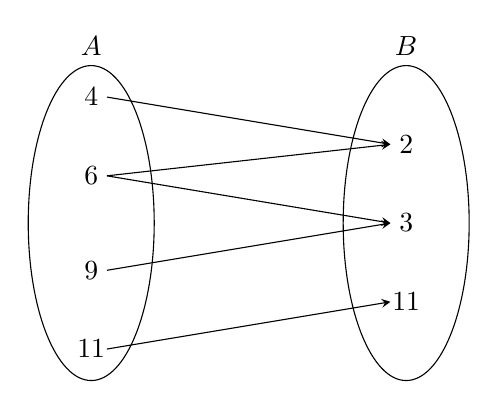
\begin{tikzpicture}[>=stealth]
\draw(2,0)ellipse[x radius=0.8cm,y radius=2cm]
(2,0)node[]{$3$}
(2,-1)node[]{$11$}
(2,1)node[]{$2$};
\draw(-2,0)ellipse[x radius =0.8cm, y radius = 2cm]
(-2,1.6)node[]{$4$}
(-2,0.6)node[]{$6$}
(-2,-0.6)node[]{$9$}
(-2,-1.6)node[]{$11$}
(-2,2)node[above]{$A$}
(2,2)node[above]{$B$};
\draw[->](-1.8,1.6)--(1.8,1);
\draw[->](-1.8,0.6)--(1.8,1);
\draw[->](-1.8,0.6)--(1.8,0);
\draw[->](-1.8,-0.6)--(1.8,0);
\draw[->](-1.8,-1.6)--(1.8,-1);
\end{tikzpicture}
\end{figure}
\vspace{0.6cm}






Consider the relation is equal to from $X$ to $Y$.
\begin{figure}[H]
\centering
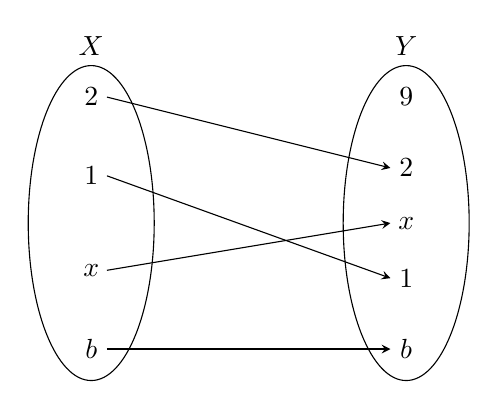
\begin{tikzpicture}[>=stealth]
\draw(-2,0)ellipse[x radius = 0.8cm, y radius = 2cm]
(2,1.6)node[]{$9$}
(2,0.7)node[]{$2$}
(2,0)node[]{$x$}
(2,-0.7)node[]{$1$}
(2,-1.6)node[]{$b$};
\draw(2,0)ellipse[x radius = 0.8cm, y radius = 2cm]
(2,2)node[above]{$Y$}
(-2,2)node[above]{$X$}
(-2,1.6)node[]{$2$}
(-2,0.6)node[]{$1$}
(-2,-0.6)node[]{$x$}
(-2,-1.6)node[]{$b$};
\draw[->](-1.8,1.6)--(1.8,0.7);
\draw[->](-1.8,0.6)--(1.8,-0.7);
\draw[->](-1.8,-0.6)--(1.8,0);
\draw[->](-1.8,-1.6)--(1.8,-1.6);
\end{tikzpicture}
\end{figure}



\vspace{0.4cm}
Here we should be concerned with relations of the type where each element in the first set is related to one element in the second set.\\

This relation is called a function or a mapping.\\




%mapping 1
\begin{figure}[H]
\centering
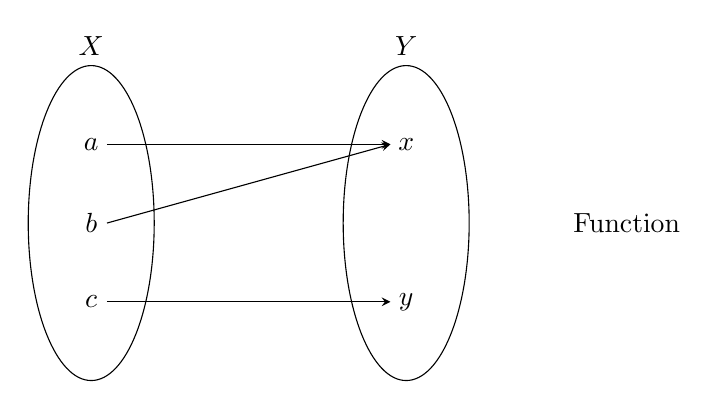
\begin{tikzpicture}[>=stealth]
\draw(2,0)ellipse[x radius=0.8cm,y radius=2cm]
(2,-1)node[]{$y$}
(2,1)node[]{$x$};
\draw(-2,0)ellipse[x radius =0.8cm, y radius = 2cm]
(-2,1)node[]{$a$}
(-2,0)node[]{$b$}
(-2,-1)node[]{$c$}
(-2,2)node[above]{$X$}
(2,2)node[above]{$Y$};
\draw[->](-1.8,1)--(1.8,1);
\draw[->](-1.8,0)--(1.8,1);
\draw[->](-1.8,-1)--(1.8,-1);
\draw(4,0)node[right]{Function};
\end{tikzpicture}
\end{figure}
\vspace{0.8cm}




% MAPPING 2
\begin{figure}[H]
\centering
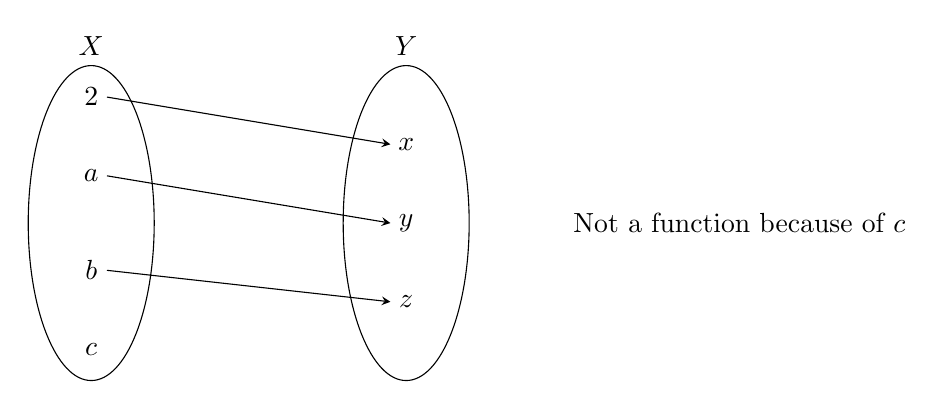
\begin{tikzpicture}[>=stealth]
\draw(2,0)ellipse[x radius=0.8cm,y radius=2cm]
(2,0)node[]{$y$}
(2,-1)node[]{$z$}
(2,1)node[]{$x$};
\draw(-2,0)ellipse[x radius =0.8cm, y radius = 2cm]
(-2,1.6)node[]{$2$}
(-2,0.6)node[]{$a$}
(-2,-0.6)node[]{$b$}
(-2,-1.6)node[]{$c$}
(-2,2)node[above]{$X$}
(2,2)node[above]{$Y$};
\draw[->](-1.8,1.6)--(1.8,1);
\draw[->](-1.8,0.6)--(1.8,0);
\draw[->](-1.8,-0.6)--(1.8,-1);
\draw(4,0)node[right]{Not a function because of $c$};
\end{tikzpicture}
\end{figure}

\vspace{2cm}







% MAPPING 3
\begin{figure}[H]
\centering
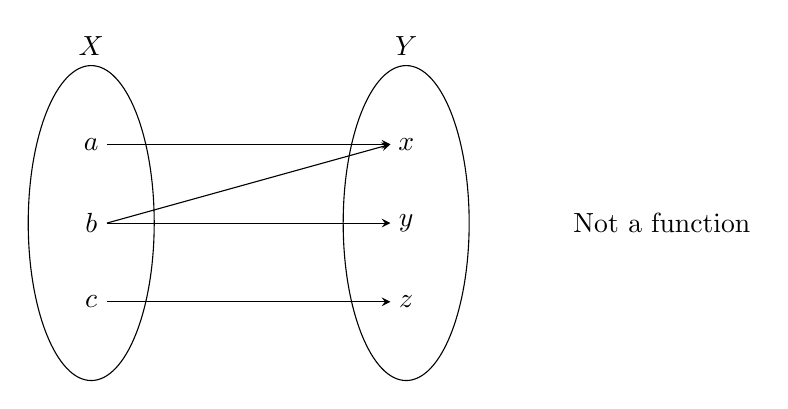
\begin{tikzpicture}[>=stealth]
\draw(2,0)ellipse[x radius=0.8cm,y radius=2cm]
(2,0)node[]{$y$}
(2,-1)node[]{$z$}
(2,1)node[]{$x$};
\draw(-2,0)ellipse[x radius =0.8cm, y radius = 2cm]
(-2,1)node[]{$a$}
(-2,0)node[]{$b$}
(-2,-1)node[]{$c$}
(-2,2)node[above]{$X$}
(2,2)node[above]{$Y$};
\draw[->](-1.8,1)--(1.8,1);
\draw[->](-1.8,0)--(1.8,1);
\draw[->](-1.8,0)--(1.8,0);
\draw[->](-1.8,-1)--(1.8,-1);
\draw(4,0)node[right]{Not a function};
\end{tikzpicture}
\end{figure}
\vspace{0.8cm}






% MAPPING 4
\begin{figure}[H]
\centering
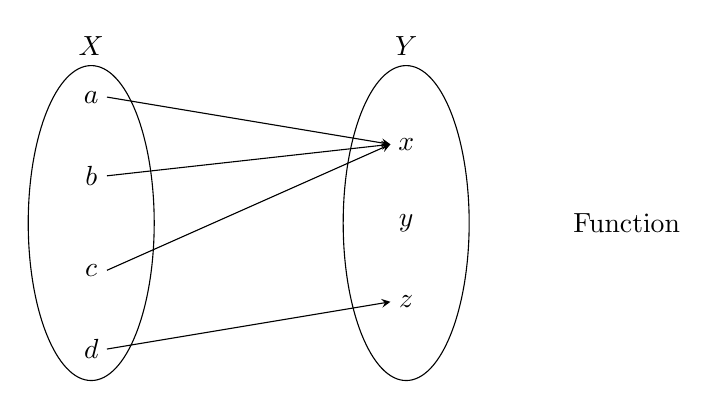
\begin{tikzpicture}[>=stealth]
\draw(2,0)ellipse[x radius=0.8cm,y radius=2cm]
(2,0)node[]{$y$}
(2,-1)node[]{$z$}
(2,1)node[]{$x$};
\draw(-2,0)ellipse[x radius =0.8cm, y radius = 2cm]
(-2,1.6)node[]{$a$}
(-2,0.6)node[]{$b$}
(-2,-0.6)node[]{$c$}
(-2,-1.6)node[]{$d$}
(-2,2)node[above]{$X$}
(2,2)node[above]{$Y$};
\draw[->](-1.8,1.6)--(1.8,1);
\draw[->](-1.8,0.6)--(1.8,1);
\draw[->](-1.8,-0.6)--(1.8,1);
\draw[->](-1.8,-1.6)--(1.8,-1);
\draw(4,0)node[right]{Function};
\end{tikzpicture}
\end{figure}
\vspace{1cm}








\subsection{Functions}
\textbf{Definition:} Let $X$ and $Y$ be two sets (not necessarily distinct). A function $f$ from $X$ to $Y$ denoted by $f:X\longrightarrow Y$ is a subset of $X\times Y$ such that for each $a\in X$ there is a unique $b\in Y$ such that $(a,b)\in f$. For each $a\in X$, the unique $b\in Y$ is called the value of $f$ at $a$ and is denoted by $b=f(a)$.\\
The other term for $b=f(a)$ is called the image of $a$ under $f$.\\
The function is also called a mapping. We say $x$ is mapped onto $x^2$ by $f$ and write $f:x\longrightarrow x^2$ if $x^2=f(x)$. This means that $f$ operates on $x$ to produce $x^2$. Often written in the form $f(x)=x^2$.\\

For example if $f(x)=x^2$ is a function then $f(3)=(3)^2=9$.\\

\textbf{Example}\\
Let $f(x)=\dfrac{x}{x+3},\hspace{0.5cm} x\neq -3$\\

Find 
\begin{enumerate}
\item $f(15)$
\item $f\bigg(-\dfrac{2}{7}\bigg)$
\item $f(a+b)$\\
\end{enumerate}

\textbf{Solution}
\begin{enumerate}
\item $f(15)=\dfrac{15}{15+3}=\dfrac{15}{18}=\dfrac{5}{6}$\\
\item $f\bigg(-\dfrac{2}{7}\bigg)=\dfrac{-\dfrac{2}{7}}{-\dfrac{2}{7}+3}=-\dfrac{2}{7}\times \dfrac{7}{19}=-\dfrac{2}{19}$\\
\item $f(a+b)=\dfrac{a+b}{a+b+c}$\\\\
\end{enumerate}







\pagebreak
\textbf{Domain and Range}\\
If $f:X\longrightarrow Y$ is a  function from $X$ onto $Y$.
\begin{enumerate}
\item We can first set $X$ the domain of the function and write $D_f=X$.
\item We call the set $Y$ the target or the Co-domain. The range of $f$ is a subset of the Co-domain and contains only the images under $f$. When the domain of a function is not explicitly stated then we take the longest set possible.\\
\end{enumerate}


\textbf{Example:}\\
State the domain of the function $f(x)=\dfrac{3}{x-5}$\\

\textbf{Solution}\\
We note that $x=5$, we should be dividing by zero which is not defined since infinity $(\infty)$ is not a real number.\\ To come up with the domain we must remove that which causes problem.\\


\begin{figure}[H]
\centering
\begin{tikzpicture}[>=stealth]
\draw(-3,0)--(3,0)
(0,0.08)--(0,-0.08)
(0,0.3)node[circle,draw,scale=0.02cm ,fill=black!0.0]{}
(0,-0.2)node[below]{$5$}
;
\draw[-Stealth](0.1,0.3)--(3,0.3);
\draw[-Stealth](-0.1,0.3)--(-3,0.3);
\end{tikzpicture}
\end{figure}

$D_f=(-\infty,5)\cup (5,\infty)$ or $D_f=\{x\in \mathbb{R}:x\neq 5\}$ or $D_f=\mathbb{R}-\{5\}$.\\\\

\textbf{Example:}\\
Determine the domain of each of the following functions:
\begin{enumerate}
\item $f(x)=\dfrac{x^2-1}{2}$
\item $g(x)=\sqrt{x}$
\item $h(x)=\dfrac{3x}{x^2-4}$
\end{enumerate}

\textbf{Solution}
\begin{enumerate}
\item Here every real number will produce another real number. Therefore there is no real number which causes problems.\\
Hence $D_f=\mathbb{R}$ the set of all real numbers.
\item So we note that if we replace $x$ by a negative number then we get an imaginary number which is not a real number. Therefore to find the domain we must remove the set of any negative real numbers.\\

\begin{figure}[H]
\centering
\begin{tikzpicture}[>=stealth]
\draw(-3,0)--(3,0)
(0,0.08)--(0,-0.08)
(0,0.3)node[circle,draw,scale=0.02cm ,fill=black!100]{}
(0,-0.2)node[below]{$0$}
;
\draw[-Stealth](0.1,0.3)--(3,0.3);
\end{tikzpicture}
\end{figure}

$D_g=[0,\infty)$\\

$D_g=\{x\in \mathbb{R}:x\geq 0\}$

\item Here $2$ and $-2$ give us head ache. So we remove them from $\mathbb{R}$.
\begin{figure}[H]
\centering
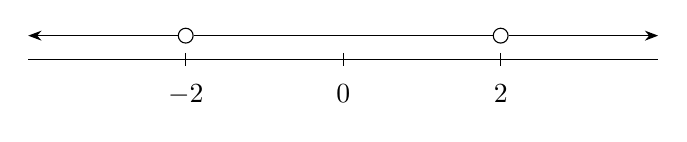
\begin{tikzpicture}[>=stealth]
\draw(-4,0)--(4,0)
(-2,0.08)--(-2,-0.08)
(0,0.08)--(0,-0.08)
(2,0.08)--(2,-0.08);
\draw(-2,-0.2)node[below]{$-2$}
(0,-0.2)node[below]{$0$}
(2,-0.2)node[below]{$2$}
(-2,0.3)node[circle,draw,scale =0.02cm, fill=black!0.0]{}
(2,0.3)node[circle,draw,scale = 0.02cm, fill = black!0.0]{}
;
\draw(0,0.3)--(1.9,0.3);
\draw[-Stealth](2.1,0.3)--(4,0.3);
\draw[-Stealth](-2.1,0.3)--(-4,0.3);
\draw(0,0.3)--(-1.9,0.3);
\end{tikzpicture}
\end{figure}

$D_h=(-\infty,-2)\cup (-2,2)\cup (2,\infty)$\\

$D_h=\mathbb{R}-\{-2,2\}$\\
\end{enumerate}


\textbf{Examples}
\begin{enumerate}
\item If $f(x)=\sqrt{ax+b}$. Then\\

$D_f: ax+b\geq 0$\\

$\implies \hspace{0.4cm} x\geq \dfrac{-b}{a}$\\

\item If $g(x)=\dfrac{ax}{bx+c}$\\

$D_g: x=\dfrac{-c}{b}$\\

Its to solve the equation $bx+c=0$ to get $x=\dfrac{-c}{b}$.\\

\item If $h(x)=ax+b$\\

$D_h=x\in \mathbb{R}$\\
All real numbers.\\
\end{enumerate}



\textbf{Range}\\

\textbf{Example}\\
Let $X=\{-4,-3,-2,-1,0,1,2,3,4\}$\\

Let $Y=\{0,1,2,3,4,\cdots\cdots\cdots, 20\}$\\

Let $f:X\longrightarrow Y$ be defined by $f(x)=x^2+1$. Find the range of $f$.\\\\

\textbf{Solution}\\
$f(-4)=(-4)^2+1=16+1=17=f(4)$\\

$f(-3)=(-3)^2+1=9+1=10=f(3)$\\

$f(-2)=(-2)^2+1=4+1=5=f(2)$\\

$f(-1)=(-1)^2+1=1+1=2=f(1)$\\

$f(0)=0^2+1=0+1=1$\\


Images are 1, 2, 5, 10, 17 $\implies R_f=\{1,2,5,10,17\}$\\\\


\textbf{Example}\\
Determine the domain and range of each of the following functions
\begin{enumerate}
\item $f(x)=3x+2$
\item $g(x)=2+\sqrt{2x-3}$
\item $h(x)=\dfrac{2}{x^2+1}$
\item $p(x)=|x-2|-3$\\
\end{enumerate}


\textbf{One-to-One}\\
\textbf{Definition:} A function $f:X\longrightarrow Y$ is one-to-one. If whenever $x_1$ and $x_2$ are distinct elements of $X$ then $f(x_1)\neq f(x_2)$.\\

Equivalently a function is one-to-one if $f(x_1)=f(x_2)\implies x_1=x_2$.\\

\textbf{Example}\\
Determine whether the function $f(x)=\dfrac{6x-4}{2x-3}$ is one-to-one.\\

\textbf{Proof:}\\
Suppose that $f(x_1)=f(x_2).$ Then
\begin{align*}
\frac{6x_1-4}{2x_1-3} & = \frac{6x_2-4}{2x_2-3}\\
\implies (6x_1-4)(2x_2-3) & = (6x_2-4)(2x_1-3)\\
\implies 12x_1x_2-18x_1-8x_2+12 & = 12x_1x_2-18x_2-8x_1+12\\
\implies -18x_1-8x_2 & = -18x_2-8x_1\\
\implies 18x_2-8x_2 & = 18x_1-8x_1\\
\implies 10x_2 &=10x_1\\\\
\therefore x_2 &=x_1\\
\end{align*}

Since $f(x_1)=f(x_2)\implies x_1=x_2$ then $f(x)=\dfrac{6x-4}{2x-3}$ is a one-to-one.\\\\


\textbf{Example}
\begin{enumerate}
\item Show that $f(x)=\dfrac{4}{7}x+8$ is one-to-one.

\textbf{Proof:}\\
 Suppose that $f(a)=f(b)$. Then $\dfrac{4}{7}a+8=\dfrac{4}{7}b+8\implies \dfrac{4}{7}a=\dfrac{4}{7}b\implies a=b$.\\
 Hence $f(x)=\dfrac{4}{7}x+8$ is one-to-one.\\
 
\item $f(x)=x^2-2x-3$\\

\textbf{Proof}\\
Suppose that $f(a)=f(b)$. Then
\begin{align*}
a^2-2a-3 & = b^2-2b-3\\
\implies a^2-2a & = b^2-2b\\
\implies a^2-b^2-2a+2b & =0\\
\implies (a-b)(a+b)-2(a-b) & = 0\\
\implies (a-b)(a+b-2) &=0\\
\end{align*}
Either $a-b=0$ or $a+b-2=0$\\
i.e $a=b$ or $a=2-b$.\\
\end{enumerate}



\subsection{Even and Odd functions}
\textbf{Definition:}\\
A function $f$ is called an even function if $f(-x)=f(x)$.\\

e.g the function $f(x)=x^2$ is even since $f(-x)=(-x)^2=x^2=f(x)$.\\

\textbf{Definition:}\\
A function $f$ is called an odd function if $f(-x)=-f(x)$.\\

e.g $f(x)=x^3+x$ is odd. Since 
\begin{align*}
f(-x) & = (-x)^3+(-x)=-x^3-x\\
      & = -(x^3+x)\\
      & = -f(x)\\
\end{align*}


\textbf{Example}\\
Determine whether each of the following functions is even, odd or neither
\begin{enumerate}
\item $f(x)=3x^4-2x^2$
\item $f(x)=x^3+x-2$
\item $f(x)=2x^3-\dfrac{1}{x}$\\
\end{enumerate}


\textbf{Solution}
\begin{enumerate}
\item $f(x)=3x^4-2x^2$
\begin{align*}
\implies \hspace{0.5cm} f(-x) & = 3(-x)^4-2(-x)^2\\
      & = 3x^4-2x^2\\
      & = f(x)
\end{align*}
i.e $f(-x)=f(x)$ which implies that $f(x)=3x^4-2x^2$ is even.\\

\item $f(x)=x^3+x-2$
\begin{align*}
\implies \hspace{0.5cm} f(-x) & = (-x)^3+(-x)-2\\
                              & = -x^3-x-2\\
                              & = -(x^3+x+2)
\end{align*}
Not even and not odd.\\

\item $f(x)=2x^3-\dfrac{1}{x}$
\begin{align*}
\implies \hspace{0.5cm} f(-x) & = 2(-x)^3-\frac{1}{(-x)}\\
                              & =-2x^3+\frac{1}{x}\\
                              & = -\big(2x^3-\frac{1}{x}\big)\\
                              & = -f(x)\hspace{0.5cm}\text{it is odd}\\
\end{align*}
\end{enumerate}




\subsection{Inverse Functions}
The inverse function of $f(x)$ is denoted by $f^{-1}(x)$. To find the inverse of a function $f$, we write $y=f(x)$ and solve the equation for $x$.\\
$f^{-1}(x)$ then is obtained by replacing $y$ by $x$.\\\\

\textbf{Example}
\begin{enumerate}
\item Find the inverse of $f(x)=\dfrac{2x-21}{3}$
\begin{align*}
\text{So, let}\hspace{0.5cm} y &=\frac{2x-21}{3}\\
               \implies 3y & = 2x-1\\
               \implies x & =  \frac{3y+1}{2}\\\\
               \therefore f^{-1}(x) & = \frac{3x+1}{2}\\
\end{align*}

\item Let $f(x)=\dfrac{x-c}{x+2}$ where $c$ is constant
\begin{enumerate}
       \item find $c$, if $f(5)=\dfrac{3}{2}$
       \item find $f^{-1}(x)$
       \item state the value of $x$ for which $f^{-1}$ is undefined.
\end{enumerate}






\pagebreak

\textbf{Solution}
\begin{enumerate}
         \item $f(5)=\dfrac{3}{2}=\dfrac{5-c}{5+2}$
\begin{align*}
\implies \frac{3}{2} & = \frac{5-c}{7}\\
\implies 5-c & = \frac{21}{2}\\
\implies c & = 5-\frac{21}{2}\\\\
\therefore c & = -\frac{11}{2}
\end{align*}
Then our function is $f(x)=\dfrac{x-(-\frac{11}{2})}{x+2}=\dfrac{2x+11}{2x+4}$\\

\item Let $y=\dfrac{2x+11}{2x+4}$
\begin{align*}
\implies 2xy+4y & = 2x+11\\
\implies 2x(y-1) & = 11-4y\\
\implies x & = \frac{11-4y}{2(y-1)}\\\\
\therefore f^{-1}(x) & =\frac{11-4x}{2(x-1)}\\
\end{align*}

\item $x=1$ makes $f^{-1}(x)$ undefined.\\
\end{enumerate}

\item Let $g(x)=x^2$
\begin{enumerate}
     \item Does the function $g(x)$ have an inverse?
     \item What can you do to the function in order to have an inverse?\\
\end{enumerate}

\textbf{Solutions}
\begin{enumerate}
       \item This shows that each element in the domain will have two different elements in the range. Therefore $g^{-1}(x)=\pm \sqrt{x}$ is not a function. Hence $g(x)=x^2$ has no inverse.
       \item The problem in this function is that it is not one-to-one. Therefore we have to redefine the domain of the function so that the given domain of the function $g(x)=x^2$ is one-to-one.\\
e.g If we restrict the domain i.e $D_g=[0,\infty)$ is the domain of the function, then the function is one-to-one and so has an inverse $$g^{-1}(x)=\sqrt{x}$$.
The second possibility to make $D_g=(-\infty,0]$

\begin{figure}[H]
\centering
\begin{tikzpicture}[>=stealth]
\draw[-Stealth](-2,0)--(2,0);
\draw[-Stealth](0,-1)--(0,2);
\draw[thick,cyan] (0,0)parabola(-2,2);
\draw(-1.5,1)node[left]{$g^{-1}(x)=-\sqrt{x}$}
(0,2.01)node[above]{$y$}
(2.01,0)node[right]{$x$};
\end{tikzpicture}
\end{figure}

In this case $g^{-1}(x)=-\sqrt{x}$.\\
\end{enumerate}
\end{enumerate}



\subsection{Composite Functions}
\textbf{Definition:} Let $f:X\longrightarrow Y$ and $g:Y\longrightarrow Z$ be two functions. Then the composite function $fog$ is a function $X\longrightarrow Z$ given by $(fog)(x)=f(g(x))$ and it is read as $f$ of $g$. That is first evaluate $g$ on $X$ and the $f$ on $g(x)$.\\

\textbf{Note:} that the domain of $g$ is the target of $f$.\\

\textbf{Example:}\\
Let $f:\mathbb{R}\longrightarrow \mathbb{R}$ and $g:\mathbb{R}\longrightarrow \mathbb{R}$ be functions defined by $f(x)=3x^2+x-2$, $g(x)=\dfrac{1}{x}$.\\

Then
\begin{enumerate}
\item[]
\begin{enumerate}
      \item $(gof)(x)=g(f(x))=\dfrac{1}{f(x)}=\dfrac{1}{3x^2+x-2}$\\
      \item $(fog)(x)=f(g(x))=3\bigg(\dfrac{1}{x}\bigg)^2+\bigg(\dfrac{1}{x}\bigg)-2=\dfrac{3}{x^2}+\dfrac{1}{x}-2$\\
      
      We see from (a) and (b) that in general $fog\neq gof$.\\
\end{enumerate}
\end{enumerate} 



\textbf{Examples}
\begin{enumerate}
\item Let $f(x)=\dfrac{3x}{3-x}$ and $h(x)=\dfrac{1}{x^2+1}$
\begin{enumerate}
      \item Find $(hof)(x)$
      \item Solve $(foh)(x)=1$
\end{enumerate}

\item Let $f(x)=\dfrac{3x}{3-x}$ and $g(x)=\dfrac{1}{x}$. Find $(fog)^{-1}(x)$.\\\\
\end{enumerate}














\pagebreak
% QUADRATIC FUNCTIONS
\section{QUADRATIC FUNCTIONS}



\subsection{Roots of a Quadratic Equation }

An equation of the form $ax^2+bx+c=0$ where $a, b$ and $c$ are constants is called quadratic equation. This equation has at most two solutions.\\

\textbf{Example:} Solve the equation $x^2+5x+6=0$.\\

\textbf{Solution:} Factorizing
\begin{align*}
x^2+3x+2x+6 & = 0\\
x(x+3)+2(x+3) & =0\\
\implies (x+3)(x+2) & = 0\\\\
\implies \text{either}\hspace{0.4cm} x+3=0\hspace{0.4cm} &\text{or}\hspace{0.4cm} x+2=0\\
\implies \text{either}\hspace{0.4cm} x=-3\hspace{0.4cm} & \text{or}\hspace{0.4cm} x=-2\\
\end{align*}



The other method of solving a quadratic equation is by completing the squares. To do this observe that \hspace{0.2cm}$(x+p)^2=x^2+2px+p^2$.\hspace{0.2cm} But $$p^2=\bigg[\frac{1}{2}(2p)\bigg]^2$$
In other words a complete square is such that the last term $p^2$ is the square of $\dfrac{1}{2}$ the middle part $2p$.\\

Our quadratic equation has the form \hspace{0.2cm}$ax^2+bx+c=0$\\

To complete the square write \hspace{0.2cm}$ax^2+bx=-c$
$$\implies x^2+\frac{b}{a}x=-\frac{c}{a}$$
middle constant is $\dfrac{b}{a}$ half of $\dfrac{b}{a}$ is $\dfrac{b}{2a}$.
\begin{align*}
\implies x^2+\frac{b}{a}x+\bigg(\frac{b}{2a}\bigg)^2 & =\frac{-c}{a}+\bigg(\frac{b}{2a}\bigg)^2\\\\
\implies \bigg(x+\frac{b}{2a}\bigg)^2 & = \frac{-c}{a}+\frac{b^2}{4a^2}\\\\
\implies \bigg(x+\frac{b}{2a}\bigg)^2 & =\frac{-4ac+b^2}{4a^2}
\end{align*}

Take the square root.
\begin{align*}
x+\frac{b}{2a} & = \pm \sqrt{\dfrac{b^2-4ac}{4a^2}}\\
\implies x & = \frac{-b}{2a}\pm \frac{\sqrt{b^2-4ac}}{\sqrt{4a^2}}\\
           & = \frac{-b}{2a} \pm \frac{\sqrt{b^2-4ac}}{2a}\\
\implies x & = \frac{-b\pm \sqrt{b^2-4ac}}{2a}\\\\
\text{i.e either}\hspace{0.3cm} x &=\frac{-b+\sqrt{b^2-4ac}}{2a}\hspace{0.3cm}  \text{or} \hspace{0.3cm} x=\frac{-b-\sqrt{b^2-4ac}}{2a}\\
\end{align*}






\subsection{Quadratic Equation}
$ax^2+bx+c=0$ is a quadratic equation, then its roots are given by $x=\dfrac{-b+\sqrt{b^2-4ac}}{2a}$ or $x=\dfrac{-b-\sqrt{b^2-4ac}}{2a}$\\\\

\textbf{Example:}\\
Solve the equation $2x^2-5x+1=0$\\

\textbf{Solution:}\\
In this case it is difficult to factorize $2x^2-5x+1$, we then use the formula to solve the equation $2x^2-5x+1=0$.\\\\
We have that $a=2, b=-5, c=1$. Thus
\begin{align*}
x= &\frac{-(-5)+\sqrt{(-5)^2-4(2)(1)}}{2(2)}=\frac{5+\sqrt{17}}{4}\\
&\text{or}\\
x = & \frac{-(-5)-\sqrt{(-5)^2-4(2)(1)}}{2(2)}=\dfrac{5-\sqrt{17}}{4}\\
\end{align*}


Now, let $\alpha$ and $\beta$ be the roots of the equation $ax^2+bx+c=0$. Then by the formula $\alpha = \dfrac{-b+\sqrt{b^2-4ac}}{2a}$ and $\beta =\dfrac{-b-\sqrt{b^2-4ac}}{2a}$.\\\\

Adding the two roots gives
\begin{align*}
\alpha + \beta & = \frac{-b+\sqrt{b^2-4ac}}{2a}+\frac{-b-\sqrt{b^2-4ac}}{2a}\\\\ 
               & = \frac{-b+\sqrt{b^2-4ac}-b-\sqrt{b^2-4ac}}{2a}\\
               & = \frac{-2b}{2a}\\\\
\therefore \hspace{0.6cm} \alpha + \beta  & =\frac{-b}{a}\\
\end{align*}



Multiplying the two roots we obtain
\begin{align*}
\alpha \beta & = \Bigg(\frac{-b+\sqrt{b^2-4ac}}{2a}\Bigg)\Bigg(\frac{-b-\sqrt{b^2-4ac}}{2a}\Bigg)\\\\
             & = \frac{b^2-b\sqrt{b^2-4ac}-b\sqrt{b^2-4ac}-(b^2-4ac)}{4a^2}\\\\
             & = \frac{4ac}{4a^2}=\frac{c}{a}\\\\
\therefore \hspace{0.6cm} \alpha \beta & = \frac{c}{a}\\
\end{align*}

Thus, if $\alpha$ and $\beta$ are the roots of the equation $ax^2+bx+c=0$, then $\alpha +\beta =\dfrac{-b}{a}$ and $\alpha \beta =\dfrac{c}{a}$.\\\\


\textbf{Example:}\\
Let $\alpha$ and $\beta$ be the roots of the equation $3x^2-7x+1=0$.\\
Find
\begin{enumerate}
\item $\alpha +\beta$
\item $\alpha \beta$\\
\end{enumerate}


\textbf{Solution}
\begin{enumerate}
\item $\alpha +\beta = \dfrac{-b}{a}=\dfrac{-(-7)}{3}=\dfrac{7}{3}$\\

\item $\alpha \beta = \dfrac{c}{a}=\dfrac{1}{3}$\\
\end{enumerate}



\begin{align*}
(\alpha + \beta )^2 &= (\alpha +\beta)(\alpha +\beta)\\
                    &= \alpha^2+\alpha \beta + \alpha \beta +\beta^2\\
                    & = \alpha^2+2\alpha \beta + \beta^2\\
                    &= \alpha^2+\beta^2+2\alpha \beta\\\\
\implies \hspace{0.6cm} \alpha^2+\beta^2 & = (\alpha +\beta)^2-2\alpha \beta\\
\end{align*}


\textbf{Example}\\
Let $\alpha$ and $\beta$ be the roots of the equation $7x^2+2x-5=0$. Find
\begin{enumerate}
\item[]
\begin{enumerate}
\item $\dfrac{1}{\alpha}+\dfrac{1}{\beta}$
\item $\alpha^2+\beta^2$
\item $\dfrac{\alpha}{\beta}+\dfrac{\beta}{\alpha}$
\item $\alpha -\beta$\\
\end{enumerate}
\end{enumerate}


\textbf{Solution}\\

$7x^2+2x-5=0$\\

$\therefore\hspace{0.5cm} a=7, b=2, c=-5$\\

$\implies \hspace{0.4cm} \alpha +\beta = \dfrac{-b}{a}=\dfrac{-2}{7}$\\

$\implies \hspace{0.4cm} \alpha \beta =\dfrac{c}{a}=\dfrac{-5}{7}$\\

\begin{enumerate}
\item[]
\begin{enumerate}
\item $\dfrac{1}{\alpha}+\dfrac{1}{\beta}=\dfrac{\beta +\alpha}{\alpha \beta}=\dfrac{-\dfrac{2}{7}}{-\dfrac{5}{7}}=\dfrac{2}{5}$\\
\item $\alpha^2+\beta^2$ using the identity $\alpha^2+\beta^2=(\alpha+\beta)^2-2\alpha \beta$, we have that\\

$\alpha^2+\beta^2=\bigg(\dfrac{-2}{7}\bigg)^2-2\bigg(\dfrac{-5}{7}\bigg)=\dfrac{4}{47}+\dfrac{10}{7}=\dfrac{4+70}{49}$\\

$\therefore \hspace{0.5cm} \alpha^2+\beta^2=\dfrac{74}{49}$\\
\item $\dfrac{\alpha}{\beta}+\dfrac{\beta}{\alpha}=\dfrac{\alpha^2+\beta^2}{\alpha \beta}=\dfrac{74/49}{-5/7}=-\dfrac{74}{35}$\\
\item $\alpha-\beta$
\begin{align*}
\text{Note that}\hspace{0.4cm} (\alpha-\beta)^2 & = \alpha^2-2\alpha \beta +\beta^2\\
                                                & = (\alpha^2+\beta^2)-2\alpha \beta\\
                                                & = (\alpha + \beta)^2-2\alpha \beta -2\alpha \beta\\
                                                & = (\alpha + \beta)^2-4\alpha \beta\\
\end{align*}
Therefore, $(\alpha-\beta)^2=\bigg(\dfrac{-2}{7}\bigg)^2-4\bigg(\dfrac{-5}{7}\bigg)=\dfrac{4}{49}+\dfrac{20}{7}=\dfrac{4+140}{49}=\dfrac{144}{49}$
$$\therefore\hspace{0.5cm} \alpha -\beta =\pm \sqrt{\frac{144}{49}}$$
$\implies\hspace{0.4cm} \alpha-\beta=\dfrac{12}{7}$ or $\alpha-\beta=-\dfrac{12}{7}$.\\
\end{enumerate}
\end{enumerate}


\textbf{Example:}\\
Let $\alpha$ and $\beta$ be the roots of the equation $2x^2-x+3=0$. Find an equation whose roots are $\alpha^2+1$ and $\beta^2+1$. $$2x^2-x+3=0$$ $$a=2, b=-1, c=3$$ $$\alpha=-\frac{1}{2}\hspace{0.3cm}\text{and}\hspace{0.3cm} \alpha \beta = \frac{3}{2}$$
The roots of the new equation are $p=\alpha^2+1$ and $q=\beta^2+1$. We need to find their sum $p+q$ and their product $pq$.\\

The new equation is of the form  \hspace{0.2cm}$x^2-(p+q)x+pq=0$.\hspace{0.2cm}
Now,
\begin{align*}
p+q & =(\alpha^2+1)+(\beta^2+1)\\
    & = \alpha^2+\beta^2+2\\
    & = (\alpha +\beta)^2-2\alpha \beta +2\\
    & = \bigg(-\dfrac{1}{2}\bigg)^2-2\bigg(\dfrac{3}{2}\bigg)+2\\
    & = \dfrac{1}{4}-3+2=\dfrac{1}{4}-1\\
    & = \dfrac{-3}{4}
\end{align*}


\begin{align*}
pq & =(\alpha^2+1)(\beta^2+1)\\
   & = \alpha^2(\beta^2+1)+1(\beta^2+1)\\
   & = (\alpha \beta)^2+\alpha^2+\beta^2+1\\
   & = (\alpha \beta)^2+(\alpha+\beta)^2-2\alpha \beta +1\\\\
\therefore \hspace{0.4cm} pq & = \bigg(\frac{3}{2}\bigg)^2+\bigg(\frac{1}{3}\bigg)^2-2\bigg(\frac{3}{2}\bigg)+1\\
                             & = \frac{9}{4}+\frac{1}{4}-3+1\\
                             & = \frac{10-8}{4}\\
                             & = \frac{1}{2}\\
\end{align*}


Thus the equation is
\begin{align*}
x^2-\bigg(\dfrac{-3}{4}\bigg)x+\dfrac{1}{2} & = 0\\
x^2+\dfrac{3}{4}x+\frac{1}{2} & = 0\\
\implies \hspace{0.4cm} 4x^2+3x+2 & =0\\
\end{align*}




\textbf{Example}\\
Given the equation $3x^2+8x+d=0$. Find the value of $d$ if the roots of this equation differ by 2.\\

\textbf{Solution}\\
Let $\alpha$ and $\beta$ be the roots of $3x^2+8x+d=0$ then $\alpha +\beta =\dfrac{-8}{3}$ and $\alpha \beta =\dfrac{d}{3}$.\\

Now, $\alpha - \beta = 2$
\begin{enumerate}
\item[] $\alpha +\beta=\dfrac{-8}{3}\cdots\cdots\cdots (1)$\\

\item[]$\alpha -\beta = 2\cdots\cdots\cdots (2)$\\
\end{enumerate}


\begin{align*}
\implies\hspace{0.4cm} \beta & = \alpha -2\\\\
\implies \hspace{0.4cm} \alpha+\alpha-2 & = \frac{-8}{3}\\\\
\implies \hspace{0.4cm} 2\alpha  = \frac{-8}{3}+2 & =\frac{-8+6}{3}\\
\end{align*}
$$\therefore \hspace{0.4cm} \alpha=\frac{-1}{3}$$\\


\begin{align*}
\frac{-1}{3}-\beta &=2\\\\
\implies \hspace{0.4cm} \beta =\frac{-1}{3}-2 & = \frac{-1-6}{3}\\\\
\therefore \hspace{0.4cm} \beta &=\frac{-7}{3}\\ 
\end{align*}

\begin{align*}
\alpha \beta & = \frac{d}{3}\\\\
\bigg(\frac{-1}{3}\bigg)\bigg(\frac{-7}{3}\bigg) & = \dfrac{d}{3}\\\\
\frac{7}{9} & = \frac{d}{3}
\implies \hspace{0.5cm} d=\frac{7}{3}\\\\
\end{align*}








\subsection{The Discriminant}
The roots of $ax^2+bx+c=0$ $$x=\frac{-b\pm \sqrt{b^2-4ac}}{2a}$$
Let $D=b^2-4ac$ then $x=\dfrac{-b\pm \sqrt{D}}{2a}$.\\

The nature of the roots of the quadratic equation $ax^2+bx+c=0$ is determined by the term $D=b^2-4ac$, where $a,b$ and $c$ are real numbers.\\

The term $D=b^2-4ac$ is called the discriminant.

\begin{enumerate}
\item When $D>0$ (i.e $b^2-4ac>0$) then the two roots of the equation are real numbers and are distinct.\\

\textbf{Example:}\\
For what values of $p$ will the equation $3x^2+px+3=0$ have real and distinct roots.\\

\textbf{Solutions:}\\
Since the roots must be real and distinct then the discriminant must be greater than zero. i.e $D=b^2-4ac>0$ but $a=3, b=p, c=3$\\

Thus, $p^2-4(3)(3)>0\implies p^2-36>0\implies (p-6)(p+6)>0$
$$(-\infty,-6)\cup (6,\infty)$$

\item When $D=b^2-4ac=0$, then the two roots of the equation are real numbers and they are equal i.e there is only one solution to the equation.\\

\textbf{Example:}\\
For what values of $k$ will the equation $kx^2+(k+1)x+k=0$ have real and equal roots.\\

\textbf{Solution}\\
If the roots are real and equal then the discriminant is zero. i.e $b^2-4ac=0$.\\
We have that $a=k, b=k+1, c=k$, that is 
\begin{align*}
(k+1)^2-4(k)(k) & = 0\\
k^2+2k+1-4k^2 & =0\\
-3k^2+2k+1 & = 0\\
-3k^2+3k-k+1 & =0\\
\implies \hspace{0.4cm} 3k(k-1)+1(k-1) & =0\\
\implies \hspace{0.4cm} (3k+1)(k-1) & =0\\
\implies \hspace{0.4cm}3k+1=0\hspace{0.3cm} &\text{or}\hspace{0.3cm} k-1=0\\\\
\therefore \hspace{0.4cm} k=\frac{-1}{3}\hspace{0.3cm} & \text{or}\hspace{0.3cm} k=1\\
\end{align*}

\item When $D=b^2-4ac<0$, then two roots of the equation are complex conjugates.\\

\textbf{Example:}\\
Determine the nature of the roots of the equation $2x^2+2x+5=0$.\\

\textbf{Solution:}\\
To determine the nature of the roots we evaluate the discriminant $D=b^2-4ac$.\\

Now, $a=2,$ $b=2$, $c=5$\\

$\implies D=(2)^2-4(2)(5)=4-40=-36<0$\\
Since $D=-36<0$ then the roots are complex conjugates.\\
\end{enumerate}


\subsection{Quadratic Functions}
A function of the form $f(x)=ax^2+bx+c$ where $a$, $b$ and $c$ are constants is called a quadratic function. Since a quadratic function is not a rational function it is defined for all real numbers.\\
Thus, the domain of a quadratic function is $\mathbb{R}$, the whole set of real numbers.\\
Most of the properties of quadratic function can be revealed if we complete the square. Completing the square we have
\begin{align*}
f(x) & = ax^2+bx+c\\
     & = a\bigg\{x^2+\frac{b}{a}x+\frac{c}{a}\bigg\}\\
     & = a\bigg\{x^2+\frac{b}{a}x+\bigg(\frac{b}{2a}\bigg)^2-\bigg(\frac{b}{2a}\bigg)^2+\frac{c}{a}\bigg\}\\
     & = a\bigg\{\bigg(x+\frac{b}{2a}\bigg)^2-\frac{b^2}{4a^2}+\frac{c}{a}\bigg\}\\\\
\implies \hspace{0.5cm} f(x) & = a\bigg\{\bigg(x+\frac{b}{2a}\bigg)^2+\frac{4ac-b^2}{4a^2}\bigg\}\\
\end{align*}

Multiplying by $a$, we obtain
$$f(x)=a\bigg(x+\frac{b}{2b}\bigg)^2+\frac{4ac-b^2}{4a}$$

Now, let $p=\dfrac{b}{2a}$ and $q=\dfrac{4ac-b^2}{4a}$. Then every quadratic function can be expressed in the form $$f(x)=a(x+p)^2+q$$ where $a,$ $p$ and $q$ are real numbers.\\\\

\textbf{Examples}\\
Express in the form $f(x)=a(x+p)^2+q$.
\begin{enumerate}
\item $f(x)=2x^2-12x+23$
\item $g(x)=1-6x-x^2$\\
\end{enumerate}


\textbf{Solution}
\begin{enumerate}
\item So $a=2$, $b=-12$ and $c=23$\\

$\implies p=\dfrac{b}{2a}=\dfrac{-12}{2(2)}=\dfrac{-12}{4}=-3$\\

$\implies q=\dfrac{4ac-b^2}{4a}=\dfrac{4(2)(23)-(-12)^2}{4(2)}=\dfrac{184-144}{8}=\dfrac{40}{8}=5$\\

\item So, this one lets us complete the square
\begin{align*}
g(x) & = 1-6x-x^2\\
     & = -x^2-6x+1\\
     & = -1\{x^2+6x-1\}\\
     & = -1\{x^2+6x+(3)^2-(3)^2-1\}\\
     & = -1\{(x+3)^2-9-1\}\\
     & = -1\{(x+3)^2-10\}\\\\
\implies   g(x)  & = -(x+3)^2+10\\
\end{align*}
\end{enumerate}


\textbf{Example}\\
Express $f(x)=x^2-2x+3$ in the form $f(x)=a(x+p)^2+q$.
\begin{align*}
f(x) & = x^2-2x+3\\
     & = x^2-2x+(1)^2-(1)^2+3\\
     & = (x-1)^2-1+3\\\\
\implies f(x) & = (x-1)^2+2
\end{align*}

It has the line of symmetry at $x-1=0\implies x=1$\\\\

In general, for any quadratic function $f(x)=ax^2+bx+c=a(x+p)^2+q$ where $p=\dfrac{b}{2a}$ and $q=\dfrac{4ac-b^2}{4a}$
\begin{enumerate}
\item The graph of $f(x)=ax^2+bx+c$ is symmetric about the line $x=-p=\dfrac{-b}{2a}$\hspace{0.2cm}
$\text{i.e}\hspace{0.3cm} x=\dfrac{-b}{2a}$
\item If $a>0$, then the graph opens upwards and $f(x)$ has minimum value $q=\dfrac{4ac-b^2}{4a}$ when $x=\dfrac{-b}{2a}$\\

Function has a minimum point $$(-p,q)=\bigg(\dfrac{-b}{2a},\dfrac{4ac-b^2}{4a}\bigg)$$
%graph

\begin{figure}[H]
\centering
\begin{tikzpicture}[>=stealth]
\draw[scale=1,domain=-1.7:1.7,smooth,variable=\x,thick, cyan]plot({\x},{\x*\x});
\draw(0,0)node[shape=circle,scale=0.01cm,fill=cyan!,thick,draw=cyan]{};
\draw[dashed,red](0,-1)--(0,3.5)node[text=black,above]{$-p$}
(-3,0)--(3,0)node[text=black,right]{$q$};
\draw(0.6,-0.1)node[below]{$(-p,q)$};
\end{tikzpicture}
\end{figure}


\item If $a<0$, then the graph opens downwards and $f(x)$ has a maximum value\\ $q=\dfrac{4ac-b^2}{4a}$ when $x=\dfrac{-b}{2a}$
% graph


\begin{figure}[H]
\centering
\begin{tikzpicture}[>=stealth]
\draw[scale=1,domain=-1.7:1.7,smooth,variable=\x,thick,cyan]plot({\x},{-\x*\x});
\draw(0,0)node[shape=circle,scale=0.01cm,fill=cyan!,thick,draw=cyan]{};
\draw[dashed,red](0,1)--(0,-3.3)node[text=black,below]{$-p$}
(-2.5,0)--(2.5,0)node[text=black,right]{$q$};
\end{tikzpicture}
\end{figure}

maximum point \hspace{0.2cm}$(-p,q)=\bigg(\dfrac{-b}{2a},\dfrac{4ac-b^2}{4a}\bigg)$\\\\
\end{enumerate}








\pagebreak
To sketch the graph of a quadratic function
\begin{enumerate}
\item Find the $y-$intercept
\item Find the line of symmetry \hspace{0.2cm}$x=\dfrac{-b}{2a}$
\item Find either the maximum or the minimum value \hspace{0.2cm}$\dfrac{4ac-b^2}{4a}$
\item Determine whether the graph opens upwards $\bigcup$ $a>0$ or if it opens downwards $\bigcap$ if $a<0$.
\begin{enumerate}
      \item on the graph itself show the $y-$ intercept.
      \item the maximum or minimum point.
      \item if the graph crosses the $x$-axis at a rational point indicate them.\\\\
\end{enumerate}
\end{enumerate}






\textbf{Example}\\
Sketch the graph of a quadratic function $f(x)=-7+12x-3x^2$.\\

\textbf{Solution}
\begin{enumerate}
\item when $x=0$, $f(0)=-7+12(0)-3(0)^2=-7$.\\
The graph crosses the $y-$axis at $(0,-7)$
\item Note that $f(x)=-3x^2+12x-7$ since $a=-3<0$ then the graph opens downwards. Hence it has maximum.\\
Note again that $f(x)=-3(x-2)^2+5$
\item The line of symmetry is $x=2$
\item Maximum value is 5
\item The maximum point is $(2,5)$.\\
% graph


\begin{figure}[H]
\centering
\begin{tikzpicture}[>=stealth]
\draw[scale=0.5,domain=-0.1:4,smooth,variable=\x,thick,cyan]plot({\x},{-7+12*\x-3*\x*\x});
\draw[->](-1,0)--(4,0);
\draw[->](0,-3.9)--(0,4);
\draw[dashed,red](1,-3.5)--(1,4);
\draw[dashed,red](-0.1,2.5)--(4,2.5);
\draw(1,2.5)node[shape=circle,draw=cyan,scale=0.01cm,fill=cyan!,thick]{}; 
\draw(0,2.5)node[]{$-$}
(0,2.5)node[left]{$5$}
(0,-3.5)node[]{$-$}
(0,-3.5)node[left]{$-7$}
(1,-0.2)node[left]{$2$};
\end{tikzpicture}
\end{figure}

\end{enumerate}




\textbf{Example}\\
Let $g(x)=ax^2-x+1$ be a quadratic function. Given that the minimum value of $g$ is $\dfrac{7}{8}$
\begin{enumerate}
\item Find the value of $a$.
\item Sketch the graph of $g(x)$.
\item Solve the equation $g(x)=2x+6$.\\
\end{enumerate}

\textbf{Solution}
\begin{enumerate}
\item Minimum value is $\dfrac{4ac-b^2}{4a}$. Now, $b=-1$ and $c=1$
\begin{align*}
\frac{4a(1)-(-1)^2}{4a} & =\frac{7}{8}\implies \frac{4a-1}{4a}=\frac{7}{8}\\\\
\implies 8(4a-1) & = 7(4a)\\
\implies  32a-8 & = 28a\\
\implies 32a-28a & = 8\\
\implies 4a & = 8\\\\
\implies a & =2
\end{align*}
\item
\begin{enumerate}
    \item $y-$intercept $g(0)=1$.
    \item $a>0$ $g(x)$ opens upwards.
    \item minimum value is $\dfrac{7}{8}$.
    \item line of symmetry $x=\dfrac{-b}{2a}$ is $x=\dfrac{1}{4}$
% graph


\begin{figure}[H]
\centering
\begin{tikzpicture}[>=stealth]
\draw[scale=1,domain=-1:1.5,smooth,variable=\x,thick,cyan]plot({\x},{2*\x*\x-\x+1});
\draw[->](-1,0)--(4,0);
\draw[->](0,-1)--(0,4);
\draw(0,1)node[]{$-$}
(0,1)node[left]{$1$}
(0.25,0.08)--(0.25,-0.08)
(0.25,-0.1)node[below]{$\frac{1}{4}$}
(1.4,4)node[right]{$g(x)=2x^2-x+1$}
(1,0.875)node[right]{$\frac{7}{8}$};
\draw[dashed,red](0.25,0)--(0.25,4);
\draw[dashed,red](-0.5,0.875)--(4,0.875);
\end{tikzpicture}
\end{figure}


\end{enumerate}
\item $g(x)=2x+6$
\begin{align*}
\implies 
2x^2-x+1 & = 2x+6\\
2x^2-3x-5 & =0\\
2x^2+2x-5x-5 & =0\\
2x(x+1)-5(x+1) & = 0\\
\implies (2x-5)(x+1) & = 0\\\\
\text{Thus}\hspace{0.3cm} 2x-5=0\hspace{0.3cm} &\text{or}\hspace{0.3cm} x+1=0\\
\end{align*}
Hence $x=\dfrac{5}{2}$ or $x=-1$\\
\end{enumerate}






\textbf{Example}\\
A farmer has 320 meters of fencing wire. He wants to enclose a rectangular garden one side of which is a river. Find the dimensions of the maximum area possible he can fence if he does not need to fence on the side where there is a river.

%graph

\begin{figure}[H]
\centering
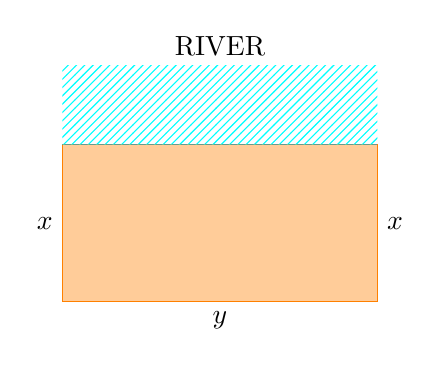
\begin{tikzpicture}[>=stealth]
\draw[orange](-2,2)--(-2,0)--(2,0)--(2,2);
\draw[cyan](-2,2)--(2,2);
\draw(-2,1)node[left]{$x$}
(0,0)node[below]{$y$}
(2,1)node[right]{$x$}
(0,3)node[above]{$\text{RIVER}$};
\path[pattern color=cyan,pattern=north east lines](-2,2)--(2,2)--(2,3)--(-2,3)--cycle;
\path[fill=orange,opacity=0.4](-2,2)--(-2,0)--(2,0)--(2,2);
\end{tikzpicture}
\end{figure}


Area $=xy$\\

Length of wire $=x+y+x\implies y+2x=320$.\\

Thus, $y=320-2x$

\begin{align*}
\text{Area} & = x(320-2x)\\
\implies A(x) & = 320-2x^2\\
              & = -2\{x^2-160x\}\\
              & = -2\{(x-80)^2-(80)^2\}\\
              & = -2\{(x-80)^2-6400\}\\
              & = -2(x-80)^2+12800
\end{align*}
Hence, the dimensions of maximum area $x=80$ and $y=12800$.\\



















\pagebreak
\section{EQUATIONS}
Solve $\dfrac{1}{x-3}+\dfrac{1}{x-2}=\dfrac{3x-8}{(x-2)(x-3)}$\\

\begin{align*}
\text{So}\hspace{0.5cm} \frac{(x-2)+(x-3)}{(x-2)(x-3)} & = \frac{3x-8}{(x-2)(x-3)}\\\\
\implies \hspace{0.5cm} \frac{2x-5}{(x-2)(x-3)} & = \frac{3x-8}{(x-2)(x-3)}\\\\
\implies \hspace{0.5cm} 2x-5 & = 3x-8\\\\
\implies \hspace{0.5cm} x & = 3\\\\ \hspace{0.5cm} \text{No solution}\\
\end{align*}

When solving equations, in most cases you must always check whether the solution obtained makes sense or not by substituting into the original equation.\\\\

\textbf{Examples:}
\begin{enumerate}
\item[(a).] $\sqrt{x}=x-2$
\item[(b).] $\sqrt{2-x}=-3$
\item[(c).] $2x+7=3\sqrt{3-2x}$
\item[(d).] $\sqrt{5x-1}=\sqrt{x}+1$\\\\
\end{enumerate}


(d). $\sqrt{5x-1}=\sqrt{x}+1$ square both sides, we get
\begin{align*}
5x-1 & = (\sqrt{x}+1)^2\hspace{0.5cm} \implies \hspace{0.5cm} 5x-1=x+2\sqrt{x} +1\\\\
\implies \hspace{0.5cm} 2\sqrt{x} & = 4x-2\hspace{0.5cm} \implies \hspace{0.5cm} \sqrt{x} = 2x-1\\\\
\implies \hspace{0.5cm} (\sqrt{x})^2 & = (2x-1)^2\hspace{0.5cm} \implies \hspace{0.5cm} x = 4x^2-4x+1\\\\
\implies \hspace{0.5cm} 4x^2-5x+1 &=0\\\\
\implies \hspace{0.5cm} 4x^2-4x-x+1 & = 0\hspace{0.5cm} \implies \hspace{0.5cm} (4x-1)(x-1)=0 \\\\
\implies \hspace{0.5cm} x=\frac{1}{4}\hspace{0.3cm} \text{or} \hspace{0.3cm} x=1\\
\end{align*}


Testing the values\\\\

For $x=\dfrac{1}{4}$\\\\
$\sqrt{\dfrac{5}{4}-1}=\sqrt{\dfrac{1}{4}}+1$\\\\

$\implies \hspace{0.5cm} \sqrt{\dfrac{5-4}{4}}=\dfrac{1}{2}+1$\\\\
$\implies \hspace{0.5cm} \dfrac{1}{2}=\dfrac{3}{2}$ false. Hence we discard $x=\dfrac{1}{4}$.\\\\

For $x=1$ $$\sqrt{5-1}=\sqrt{1}+1\hspace{0.4cm} \implies \hspace{0.4cm} \sqrt{4}=1+1\hspace{0.4cm} \implies \hspace{0.4cm} 2=2$$
Thus $x=1$ is a solution. Hence $x=1$ is the only solution.\\\\








\pagebreak
% FUNCTIONS OF THE FORM F(X) = \sqrt{X}
\section{FUNCTIONS OF THE FORM $f(x)=\sqrt{x}$}
We have already seen that the function $f(x)=\sqrt{x}$ is defined only for values of $x\geq 0$. Only non-negative values will appear for $x$.\\

\begin{table}[H]
\centering
\begin{tabular}{c|cccccccccc}
$x$ && 0 && 1 && 4 && 9 && 16\\
\hline
$f(x)=\sqrt{x}$ && 0 && 1 && 2 && 3 && 4\\
\end{tabular}
\end{table}
\vspace{0.4cm}



\begin{figure}[H]
\centering
\begin{tikzpicture}[>=stealth]
\draw[-Stealth](0,-1)--(0,4);
\draw[-Stealth](-1,0)--(8,0);
\draw[scale=0.5,domain=0:16, smooth, variable=\x,cyan]plot({\x},{sqrt(\x)})
(1,1)node[shape=circle,draw,scale=0.01cm, fill=cyan!]{}
(4,2)node[shape=circle,draw,scale=0.01cm,fill=cyan!]{}
(9,3)node[shape=circle,draw,scale=0.01cm,fill=cyan!]{}
(16,4)node[shape=circle,draw,scale=0.01cm,fill=cyan!]{}
(0,0)node[shape=circle,draw,scale=0.01cm,fill=cyan!]{}
;
\end{tikzpicture}
\end{figure}
\vspace{1cm}





\begin{enumerate}
\item Thus all the graphs of the form $f(x)=\sqrt{x}$ have the same shape of the graph below

\begin{figure}[H]
\centering
\begin{tikzpicture}[>=stealth]
\draw[-Stealth](-1,0)--(5,0);
\draw[-Stealth](0,-1)--(0,4);
\draw(3,0)node[below]{$x\geq 0$}
(4,2.1)node[right]{$f(x)=\sqrt{x}$}
;
\draw[scale=1,domain=0:4,smooth,variable=\x,thick,cyan]plot({\x},{sqrt(\x)})
;
\end{tikzpicture}
\end{figure}


\item $f(x)=-\sqrt{x}$. This is a reflection of the graph of the function $f(x)=\sqrt{x}$ in the\\ $x-$ axis.

\begin{figure}[H]
\centering
\begin{tikzpicture}[>=stealth]
\draw[-Stealth](-2,0)--(5,0);
\draw[-Stealth](0,-3)--(0,2);
\draw(3,0)node[below]{$x\geq 0$}
(4,-2.1)node[right]{$f(x)=-\sqrt{x}$}
;
\draw[scale=1,domain=0:4,smooth,variable=\x,thick,cyan]plot({\x},{-sqrt(\x)})
;
\end{tikzpicture}
\end{figure}


\item $f(x)=\sqrt{-x}$. The domain of this function is the set of all non positive real numbers $x\leq 0$, its graph below

\begin{figure}[H]
\centering
\begin{tikzpicture}[>=stealth]
\draw[-Stealth](-5,0)--(2,0);
\draw[-Stealth](0,-1)--(0,3);
\draw(-3,0)node[below]{$x\leq 0$}
(-4,2.1)node[left]{$f(x)=\sqrt{-x}$};
\draw[scale=1,domain=-4:0,smooth, variable=\x,thick,cyan]plot({\x},{sqrt(-\x)});
\end{tikzpicture}
\end{figure}


\item $f(x)=-\sqrt{-x}$. This function is a reflection of $f(x)=\sqrt{-x}$ in the $x-$ axis.\\
\begin{figure}[H]
\centering
\begin{tikzpicture}[>=stealth]
\draw[-Stealth](-5,0)--(2,0);
\draw[-Stealth](0,-3)--(0,2);
\draw(-3,0)node[below]{$x\leq 0$}
(-4,-2.1)node[left]{$f(x)=-\sqrt{-x}$};
\draw[scale=1,domain=-4:0,smooth, variable=\x,thick,cyan]plot({\x},{-sqrt(-\x)});
\end{tikzpicture}
\end{figure}
\end{enumerate}


Consider now the graph of $f(x)=\sqrt{x-2}$. To find the domain of $f$ we must solve\\ $x-2\geq 0\implies x\geq 0$.\\

\begin{figure}[H]
\centering
\begin{tikzpicture}[>=stealth]
\draw(-3,0)--(3,0)
(0,0.08)--(0,-0.08)
(0,0.3)node[circle,draw,scale=0.015cm ,fill=black!100]{}
(0,-0.2)node[below]{$2$}
;
\draw[-Stealth](0.01,0.3)--(3,0.3);
\end{tikzpicture}
\end{figure}

The range of $f$ is all the non-negative real numbers.\\

The graph of $f(x)=\sqrt{x-2}$ has the same shape as the graph of $f(x)=\sqrt{x}$. Except that the graph will start at $x=2$.\\



\begin{figure}[H]
\centering
\begin{tikzpicture}[>=stealth]
\draw[-Stealth](-1,0)--(6,0);
\draw[-Stealth](0,-1)--(0,4);
\draw(2,0)node[]{$|$}
(2,-0.2)node[below]{$2$}
(5,2.1)node[left]{$f(x)=\sqrt{x-2}$}
;
\draw[scale=1,domain=2:6,smooth,variable=\x,thick,cyan]plot({\x},{sqrt(\x-2)})
;
\end{tikzpicture}
\end{figure}



\textbf{Example}\\
Sketch $f(x)=-1+\sqrt{x}$.\\

\textbf{Solution}\\

The domain  $D_f$ is $x\geq 0$.\\

The range $R_f$ is $-1$ to $\infty$. i.e $R_f=[-1,\infty)$\\




\begin{figure}[H]
\centering
\begin{tikzpicture}[>=stealth]
\draw[-Stealth](-1,0)--(6,0);
\draw[-Stealth](0,-2)--(0,3);
\draw(1,0)node[]{$|$}
(1,-0.1)node[below]{$1$}
(0,-1)node[]{$-$}
(-0.2,-1)node[left]{$-1$}
(5,1.5)node[left]{$f(x)=-1+\sqrt{x}$}
;
\draw[scale=1,domain=0:6,smooth,variable=\x,cyan,thick]plot({\x},{-1+sqrt(\x)})
;
\end{tikzpicture}
\end{figure}
\vspace{0.5cm}




\textbf{Example}\\
State the domain and the range of each of the functions below and hence sketch the graph of the function.

\begin{enumerate}
\item $f(x)=-\sqrt{2x-1}$\\

Domain:\\
$2x-1\geq 0\implies x\geq \dfrac{1}{2}$.\\

$\therefore D_f=\bigg[\dfrac{1}{2},\infty\bigg)$

Since the sign in front of the root symbol is negative the range of $f$ must be negative numbers.\\
But when $x=\dfrac{1}{2}, y=0$.\\
Therefore the starting point is $\bigg(\dfrac{1}{2},0\bigg).$




\begin{figure}[H]
\centering
\begin{tikzpicture}[>=stealth]
\draw[-Stealth](-1,0)--(5,0);
\draw[-Stealth](0,-3)--(0,2);
\draw(0.5,0)node[]{$|$}
(0.4,-0.1)node[below]{$\dfrac{1}{2}$}
(4,-2)node[right]{$f(x)=-\sqrt{2x-1}$}
;
\draw[scale=1,domain=0.5:4,smooth,variable=\x,thick,cyan]plot({\x},{-sqrt(2*\x-1)})
;
\end{tikzpicture}
\end{figure}


\item $g(x)=-1+\sqrt{3-x}$\\

Domain of $g$: $3-x\geq 0\implies 3\geq x$\\

$D_g=(-\infty,3]$\\

Most of the values in the range will be positive.\\
However, when $x=3, y=-1$\\
The graph starts at $(3,-1)$.\\
We note that the graph will cross both $y=-1+\sqrt{3-x}$ but where it crosses the $x-$axis, $y=0$ thus $0=-1+\sqrt{3-x}\implies 1=\sqrt{3-x}\implies 3-x=1\implies x=2$.\\

It crosses the $x-$axis at $(2,0)$ and it crosses the $y-$axis when $x=0, f(0)=-1+\sqrt{3}$.\\
It crosses the $y-$axis at $(0,-1+\sqrt{3})$


\begin{figure}[H]
\centering
\begin{tikzpicture}[>=stealth]
\draw[-Stealth](-5,0)--(4,0);
\draw[-Stealth](0,-2)--(0,4);
\draw(2,0)node[]{$|$}
(2,-0.1)node[below]{$2$}
(3,-0.2)node[right]{$3$}
(3.6,-1.1)node[below]{$(3,-1)$}
(-5,2.1)node[right]{$f(x)=-1+\sqrt{3-x}$}
(-0,-1.2)node[left]{$-1$}
(0,0.73)node[]{$-$}
(0.1,0.73)node[right]{$-1+\sqrt{3}$};
\draw[scale=1,domain=-4:3,smooth,variable=\x,thick,cyan]plot({\x},{-1+sqrt(3-\x)});
\draw[dashed,red](3,-2)--(3,4)
(-5,-1)--(4,-1);
\end{tikzpicture}
\end{figure}


\item $P(x)=2-\sqrt{1+2x}$\\

$D_f=\bigg[-\dfrac{1}{2},\infty \bigg)$\\

starts at $\bigg(-\dfrac{1}{2},2\bigg)$\\

$x-$intercept, $y=0$\\
$0=2-\sqrt{1+2x}\implies 1+2x=4\implies 2x=4-1\implies 2x=3\implies x=\dfrac{3}{2}$\\

crosses the $x-$axis at $\bigg(\dfrac{3}{2},0\bigg)$\\

$y-$intercept $x=0$\\
$P(0)=2-\sqrt{1+0}=2-1=1$\\

crosses $y-$axis at $(0,1)$.


\begin{figure}[H]
\centering
\begin{tikzpicture}[>=stealth]
\draw[-Stealth](-2,0)--(5,0);
\draw[-Stealth](0,-3)--(0,4);
\draw(1.5,0)node[]{$|$}
(1.5,-0.1)node[below]{$\dfrac{3}{2}$}
(5,-2.1)node[left]{$f(x)=2-\sqrt{1+2x}$}
(0,1)node[]{$-$}
(-0.1,1)node[left]{$1$}
(-0.8,-0.1)node[below]{$-\dfrac{1}{2}$}
(0,2)node[left]{$2$};
\draw[dashed,red](-0.5,-3)--(-0.5,4)
(-2,2)--(4,2);
\draw[scale=1,domain=-0.5:5,smooth,variable=\x,thick,cyan]plot({\x},{2-sqrt(1+2*\x)})
;
\end{tikzpicture}
\end{figure}


\vspace{0.4cm}

\item $h(x)=3\sqrt{3x+2}+2$\\
\end{enumerate}















\pagebreak
\section{INEQUALITIES}
An inequality is an expression of the form $2x+3>4$ or $x\leq 7$ or $2x-1\geq 3x+2$.\\

$<,>,\leq ,\geq$ symbols found in a inequality.\\

$\bullet$ Types of inequalities:
\begin{enumerate}
\item Linear inequalities $ax+b\geq 0$.
\item Absolute value inequalities $|ax+b|<k$.
\item Quadratic inequalities $ax^2+bx+c\leq 0$.
\item Rational inequalities $\dfrac{ax+b}{cx+d}=k$.\\
\end{enumerate}

\subsection{Linear Inequalities}
Solve each of the following inequalities. Hence show on a number line
\begin{enumerate}
\item[(a).] $3x-2\leq -1$
\begin{align*}
3x-2 &\leq -1\\
\implies 3x & \leq -1+2\\
\implies x & \leq \frac{1}{3}\\\\
\therefore\hspace{0.5cm} SS: & \bigg(-\infty,\frac{1}{3}\bigg]
\end{align*}




\begin{figure}[H]
\centering
\begin{tikzpicture}[>=stealth]
\draw(-3,0)--(3,0)
(0,0.08)--(0,-0.08)
(0,0.3)node[circle,draw,scale=0.015cm ,fill=black!100]{}
(0,-0.2)node[below]{$\dfrac{1}{3}$}
;
\draw[<-](-3,0.3)--(-0.01,0.3);
\end{tikzpicture}
\end{figure}


\item[(b).] $\dfrac{2}{3}x+5>3$
\begin{align*}
\frac{2}{3}x &> 3-5\\
\implies \frac{2}{3}x & > -2\\
\implies x & > -3\\\\
\therefore \hspace{0.5cm} SS:& (-3,+\infty)
\end{align*}



\begin{figure}[H]
\centering
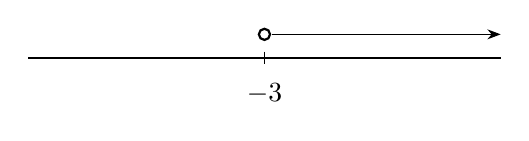
\begin{tikzpicture}[>=stealth]
\draw(-3,0)--(3,0)
(0,0.08)--(0,-0.08)
(0,0.3)node[circle,draw=black,thick,scale=0.015cm ,fill=black!0.0]{}
(0,-0.2)node[below]{$-3$}
;
\draw[-Stealth](0.09,0.3)--(3,0.3);
\end{tikzpicture}
\end{figure}


\item[(c).] $2x+3\geq 5x-2$
\begin{align*}
2x+3 & \geq 5x-2\\
\implies 2x-5x & \geq -2-3\\
\implies -3x & \geq -5\\
\implies x & \leq \frac{-5}{-3}\\
\implies x & \leq \frac{5}{3}\\\\
\therefore\hspace{0.5cm} SS:& \bigg(-\infty,\frac{5}{3}\bigg]
\end{align*}



\begin{figure}[H]
\centering
\begin{tikzpicture}[>=stealth]
\draw(-3,0)--(3,0)
(0,0.08)--(0,-0.08)
(0,0.3)node[circle,draw,thick,scale=0.015cm ,fill=black!100]{}
(0,-0.2)node[below]{$\dfrac{5}{3}$}
;
\draw[-Stealth](-0.09,0.3)--(-3,0.3);
\end{tikzpicture}
\end{figure}
\end{enumerate}



\subsection{Absolute Value Inequalities}

Recall that $|x|=
\begin{cases}
x & \text{if}\hspace{0.3cm} x\geq 0\\\\
-x & \text{if}\hspace{0.3cm} x<0\\
\end{cases}
$\\

Consider solving the inequality $|x|<k$ where $k$ is positive real number.\\
There are two cases to consider either $x$ is positive or $x$ is negative.\\

If $x>0$ then $x<k$ is the solution set.\\
Since $|x|=x$.\\
If $x<0,$ then $|x|=-x$ so that $|x|<k \implies -x<k\implies x>-k$.\\

Hence the two solutions imply that $-k<x$ and $x<k$.\\


Thus, $|x|<k$ if and only if $-k<x<k$.\\


$x>0\implies x<k$ and $x<0\implies x>-k$. Both solutions must be satisfied.




\begin{figure}[H]
\centering
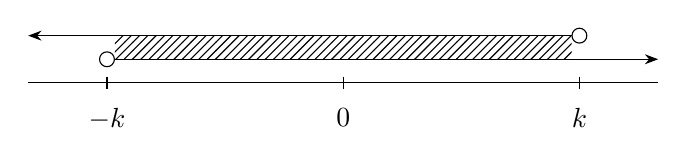
\begin{tikzpicture}[>=stealth]
\draw(-4,0)--(4,0)
(0,0.08)--(0,-0.08)
(-3,0.08)--(-3,-0.08)
(3,0.08)--(3,-0.08)
(-3,0.3)node[circle,draw,scale=0.02cm ,fill=black!0.0]{}
(3,0.6)node[circle,draw,scale=0.02cm,fill=black!0.0]{}
(0,-0.2)node[below]{$0$}
(-3,-0.2)node[below]{$-k$}
(3,-0.2)node[below]{$k$}
;
\draw[-Stealth](-2.9,0.3)--(4,0.3);
\draw[-Stealth,fill=black,below](2.9,0.6)--(-4,0.6);
\path[pattern=north east lines](-2.9,0.3)--(2.9,0.3)--(2.9,0.6)--(-2.9,0.6)--cycle;
\end{tikzpicture}
\end{figure}



Take the intersection of the two solutions: \hspace{0.2cm}$(-k,k)=\{x\in \mathbb{R}:-k<x<k\}$\\\\



\textbf{Example}\\
Find the solution set of $|2x-3|\leq 5$.\\

\textbf{Solution}\\
$|2x-3|\leq 5\implies -5\leq 2x-3\leq 5$\\

two sections\\

$-5\leq 2x-3\cdots\cdots\cdots (1)$\\

$2x-3\leq 5\cdots\cdots\cdots (2)$\\


Solve the two inequalities and take the intersection of their solution sets:\\

Now
\begin{align*}
-5 &\leq 2x-3\\
\implies -5+3 & \leq 2x\\
\implies -2 & \leq 2x\\
\implies -1 & \leq x
\end{align*}




\begin{figure}[H]
\centering
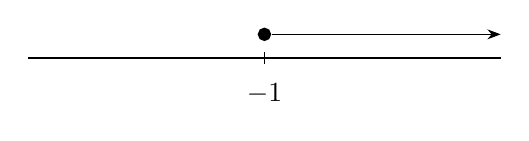
\begin{tikzpicture}[>=stealth]
\draw(-3,0)--(3,0)
(0,0.08)--(0,-0.08)
(0,0.3)node[circle,draw,thick,scale=0.015cm ,fill=black!100]{}
(0,-0.2)node[below]{$-1$}
;
\draw[-Stealth](0.09,0.3)--(3,0.3);
\end{tikzpicture}
\end{figure}
\vspace{0.4cm}



\begin{align*}
2x-3 & \leq 5\\
\implies 2x & \leq 5+3\\
\implies 2x & \leq 8\\
\implies x & \leq 4
\end{align*}





\begin{figure}[H]
\centering
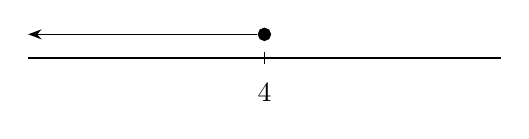
\begin{tikzpicture}[>=stealth]
\draw(-3,0)--(3,0)
(0,0.08)--(0,-0.08)
(0,0.3)node[circle,draw,thick,scale=0.015cm ,fill=black!100]{}
(0,-0.2)node[below]{$4$}
;
\draw[-Stealth](-0.09,0.3)--(-3,0.3);
\end{tikzpicture}
\end{figure}
\vspace{0.3cm}

Taking the intersection of the two solutions:



\begin{figure}[H]
\centering
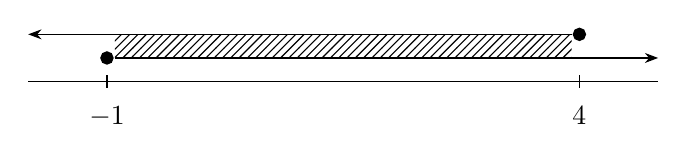
\begin{tikzpicture}[>=stealth]
\draw(-4,0)--(4,0)
(-3,0.08)--(-3,-0.08)
(3,0.08)--(3,-0.08)
(-3,0.3)node[circle,draw,thick,scale=0.015cm ,fill=black!100]{}
(3,0.6)node[circle,draw,thick,scale=0.015cm,fill=black! 100]{}
(-3,-0.2)node[below]{$-1$}
(3,-0.2)node[below]{$4$}
;
\draw[-Stealth](-2.9,0.3)--(4,0.3);
\draw[-Stealth,fill=black,below](2.9,0.6)--(-4,0.6);
\path[pattern=north east lines](-2.9,0.3)--(2.9,0.3)--(2.9,0.6)--(-2.9,0.6)--cycle;
\end{tikzpicture}
\end{figure}

There our solution set: $SS:[-1,4], \hspace{0.4cm} -1\leq x\leq 4$.\\







\pagebreak
\subsection{Quadratic Inequalities}

A quadratic inequality can be solved either by graphs or by use of tables or analytically.\\


\textbf{Example}\\
Find the values of $x$ such that $x^2+x-6<0$.\\

\textbf{Solution}
\begin{enumerate}
\item By Graph\\

Let $y=x^2+x-6$. The graph of this function is 


\begin{figure}[H]
\centering
\begin{tikzpicture}[>=stealth]
\draw[-Stealth](0,-3.5)--(0,2.5);
\draw[-Stealth](-4,0)--(2.5,0);
\draw[scale=0.5,domain=-3.5:2.5, smooth, variable=\x, thick,cyan]plot({\x},{\x*\x+\x-6});
\draw[dashed,red](-0.25,-4)--(-0.25,2.5);
\draw(1,0)node[]{$|$}
(-1.5,0)node[]{$|$}
(-1.7,-0.1)node[below]{$-3$}
(1.1,-0.1)node[below]{$2$}
(-0.3,-0.1)node[below]{$-\frac{1}{2}$};
\end{tikzpicture}
\end{figure}

$x^2+x-6<0\implies y<0$\\

Here we see that values of $y$ are negative between $-3$ and 2. Therefore the solution set is $$SS: \{x\in \mathbb{R}:-3<x<2\}$$

\item By Tables\\

Here we first find critical values. Critical values of $x$ where the factors in the given expression are zeros.\hspace{0.2cm}$x^2+x-6=0$\\

Now, \hspace{0.2cm}$(x+3)(x-2)<0$\\

critical values: \hspace{0.2cm}$x=-3$ and $x=2$\\



\begin{table}[H]
\centering
\begin{tabular}{cccccc}
& $(-5)$ & $-3$  & 0 & 2& $(3)$\\
\hline
\multicolumn{1}{c|}{$x+3$ } & $-ve$ & $|$ & $+ve$ & $|$  & $+ve$\\
\multicolumn{1}{c|}{$x-2$} & $-ve$  & $|$ & $-ve$ & $|$  & $+ve$\\
\multicolumn{1}{c|}{$(x+3)(x-2)$} & $+ve$ & $|$ & $-ve$  & $|$ & $+ve$\\
\end{tabular}
\end{table}


Thus $x^2+x-6<0$ if $-3<x<2$. Therefore the solution set is $SS:(-3,2)$.\\
\end{enumerate}



\textbf{Example}\\
Solve the inequality $2x-1<x^2-4$.
\begin{enumerate}
\item By tables
\item Analytically\\
\end{enumerate}

\textbf{Solution}
\begin{enumerate}
\item By Table: First we find critical values.\\

Now
\begin{align*}
2x-1 & < x^2-4\\
\implies 0 &< x^2-4-2x+1\\
\implies x^2-2x-3 &>0\\
\implies (x-3)(x+1)&>0
\end{align*}

Critical values $x-3=0\implies x=3$ and $x+1=0\implies x=-1$\\


\begin{table}[H]
\centering
\begin{tabular}{ccccccc}
&& $(-2)$ & $-1$ & 0 & 3 & $(4)$\\
\hline 
$(x-3)$ & \multicolumn{1}{r|}{} & $-ve$ & $|$ & $-ve$ & $|$ & $+ve$\\
$(x+1)$ & \multicolumn{1}{r|}{} & $-ve$ & $|$ & $+ve$ & $|$ & $+ve$\\
$(x-3)(x+1)$ & \multicolumn{1}{r|}{} & $+ve$ & $|$ & $-ve$ & $|$ & $+ve$\\
\end{tabular}
\end{table}

The product is positive in the interval $(-\infty,-1)$ and $(3,\infty)$. Therefore $$SS:(-\infty,-1)\cup (3,\infty)$$

\item Analytically\\
$(x-3)(x+1)>0$\\
Since the product of two factors is positive then both factors must have the same sign.\\

\textbf{case 1}\\
$x-3>0$ and $x+1>0$\\
$\implies x>3$ and $x>-1$\\
$(3,\infty)$ and $(-1,\infty)$\\

Thus we  are looking for the intersection. i.e $(3,\infty)\cap (-1,\infty)=(3,\infty)$.\\

\textbf{case 2}\\
$x-3<0$ and $x+1<0$\\
$\implies x<3$ and $x<-1$\\
$\implies (-\infty,3)\cap (-\infty,-1)=(-\infty,-1)$\\

Hence, $SS:(-\infty,-1)\cup (3,\infty)$\\
\end{enumerate}







\subsection{Rational Inequalities}
When dealing with a rational inequality avoid cross multiplying.\\

\textbf{Example}\\
Solve the inequality $\dfrac{x}{x+2}\geq 3$.\\

\textbf{Solution}\\
The best method to solve such inequality is by use of table 
\begin{align*}
\frac{x}{x+2} &\geq 3\implies \frac{x}{x+2}-3\geq 0\\\\
\implies \frac{x-3(x+2)}{(x+2)} & \geq 0\\
\implies \frac{x-3x-6}{x+2} &\geq 0\\
\implies \frac{-2x-6}{x+2} &\geq 0\\
\implies -\bigg(\frac{2x+6}{x+2}\bigg) & \geq 0\\\\
\implies \frac{2x+6}{x+2}\leq 0\\
\end{align*}

Note the factors are $2x+6$ and $x+2$.\\
Therefore the critical values are\\
$2x+6=0\implies x=-3$
$x+2=0\implies x=-2$



\begin{table}[H]
\centering
\begin{tabular}{cccccc}
& $(-4)$ & $-3$ & $(\dfrac{-5}{2})$ & $-2$ & 0\\
\hline
\multicolumn{1}{c|}{$2x+6$}  & $-ve$ & $|$ & $+ve$ & $|$ & $+ve$\\
\multicolumn{1}{c|}{$x+2$} & $-ve$ & $|$ & $-ve$ & $|$ & $+ve$\\
\multicolumn{1}{c|}{}&&&&&\\
\multicolumn{1}{c|}{$\dfrac{2x+6}{x+2}$}  & $+ve$ & $|$ & $-ve$ & $|$ & $+ve$\\
\end{tabular}
\end{table}
$$SS:[-3,-2)$$




\textbf{Examples}\\
Solve the following inequalities
\begin{enumerate}
\item[(a).] $\dfrac{x+1}{x}\leq \dfrac{1}{3}$
\item[(b).] $\dfrac{2x+1}{x-3}<\dfrac{1}{2}$\\
\end{enumerate}

\textbf{Solution}
\begin{align*}
\frac{x+1}{x} & \leq \frac{1}{3}\\
\implies \frac{x+1}{x}-\frac{1}{3} & \leq 0\\
\implies \frac{3(x+1)-x}{3x} & \leq 0\\
\implies \frac{3x+3-x}{3x} & \leq 0\\
\implies \frac{2x+3}{3x} & \leq 0\\
\end{align*}


The critical values, $2x+3=0\implies x=\dfrac{-3}{2}$ and $3x=0\implies x=0$.

\begin{table}[H]
\centering
\begin{tabular}{cccccc}
& $(-2)$ & $-\frac{3}{2}$ & $(-1)$ & 0 & $(1)$\\
\hline
\multicolumn{1}{c|}{$2x+3$}  & $-ve$ & $|$ & $+ve$ & $|$ & $+ve$\\
\multicolumn{1}{c|}{$3x$}    & $-ve$ & $|$ & $-ve$ & $|$ & $+ve$\\
\multicolumn{1}{c|}{}&&&&&\\
\multicolumn{1}{c|}{$\dfrac{2x+3}{3x}$}  & $+ve$ & $|$ & $-ve$ & $|$ & $+ve$\\
\end{tabular}
\end{table}

$$SS:\bigg[-\frac{3}{2},0\bigg)$$\\

\begin{align*}
\frac{2x+1}{x-3} & < \frac{1}{2}\\
\implies \frac{2x+1}{x-3}-\frac{1}{2} & <0\\
\implies \frac{2(2x+1)-(x-3)}{2(x-3)} & <0\\
\implies \frac{4x+2-x+3}{2(x-3)} & <0\\
\implies \frac{3x+5}{2(x-3)} & 0
\end{align*}

Critical values\\
$3x+5=0\implies x=-\dfrac{5}{3}$ and $2(x-3)=0\implies x=3$.




\begin{table}[H]
\centering
\begin{tabular}{cccccc}
& $(-2)$ & $-\frac{5}{3}$ & 0 & 3 & $(4)$\\
\hline
\multicolumn{1}{c|}{$3x+5$} & $-ve$ & $|$ & $+ve$ & $|$ & $+ve$\\
\multicolumn{1}{c|}{$2(x-3)$}  & $-ve$ & $|$ & $-ve$ & $|$ & $+ve$\\
\multicolumn{1}{c|}{}&&&&&\\
\multicolumn{1}{c|}{$\dfrac{3x+5}{2(x-3)}$} & $+ve$ & $|$ & $-ve$ & $|$ & $+ve$\\
\end{tabular}
\end{table}

$$SS:\bigg(-\frac{5}{3},3\bigg)$$\\

For $\dfrac{2x+1}{x-3}>\dfrac{1}{2}$, the solution set is $SS:\bigg(-\infty,-\dfrac{5}{3}\bigg)\cup (3,\infty)$.\\\\




\textbf{Example}\\
Find the solution set of the inequality $\bigg|\dfrac{2x}{x-3}\bigg|<\dfrac{1}{2}$.\\

\textbf{Solution}\\
Implies that $-\dfrac{1}{2}<\dfrac{2x}{x-3}<\dfrac{1}{2}$\\

This gives two inequalities to be solved $-\dfrac{1}{2}<\dfrac{2x}{x-3}$ and $\dfrac{2x}{x-3}<\dfrac{1}{2}$.\\\\

For $-\dfrac{1}{2}<\dfrac{2x}{x-3}$ we have $0<\dfrac{2x}{x-3}+\dfrac{1}{2}$\\\\

$\implies 0<\dfrac{4x+x-3}{2(x-3)}\implies 0<\dfrac{5x-3}{2(x-3)}$\\

The critical values are $x=\dfrac{3}{5}$ and $x=3$.\\\\



\begin{table}[H]
\centering
\begin{tabular}{cccccc}
& 0 & $\frac{3}{5}$ & $(2)$ & 3 & $(4)$\\
\hline
\multicolumn{1}{c|}{$5x-3$}  & $-$ & $|$ & $+$ & $|$ & $+$\\
\multicolumn{1}{c|}{$2(x-3)$} & $-$ & $|$ & $-$ & $|$ & $+$\\
\multicolumn{1}{c|}{}&&&&&\\
\multicolumn{1}{c|}{$\dfrac{5x-3}{2x-6}$} & $+$ & $|$ & $-$ & $|$& $+$\\
\end{tabular}
\end{table}

$$SS_1:\bigg(-\infty,\frac{3}{5}\bigg)\cup (3,\infty)$$\\


For $\dfrac{2x}{x-3}<\dfrac{1}{2}$, we have that $\dfrac{2x}{x-3}-\dfrac{1}{2}<0$\\\\

$$\implies \frac{4x-x+3}{2(x-3)}<0\implies \frac{3x+3}{2(x-3)}<0$$

critical values: $x=-1$ and $x=3$.\\

\begin{table}[H]
\centering
\begin{tabular}{cccccc}
& $(-2)$ & $-1$ & 0 & 3 & $(4)$\\
\hline
\multicolumn{1}{c|}{$3x+3$}  & $-$ & $|$ & $+$ & $|$ & $+$\\
\multicolumn{1}{c|}{$2x-6$}  & $-$ & $|$ & $-$ & $|$ & $+$\\
\multicolumn{1}{c|}{$\dfrac{3x+3}{2x-6}$} & $+$ & $|$ & $-$ & $|$ & $+$\\
\end{tabular}
\end{table}


$$SS_2:(-1,3)$$\\

The required solution is the intersection of $SS_1$ and $SS_2$.

$$SS:\bigg(-1,\frac{3}{5}\bigg)$$\\\\
% TO be continued






\textbf{Example}\\
Find the solution set of the inequality $\dfrac{x}{x^2-4}<0$.\\

\textbf{Solution}
$$\frac{x}{x^2-4}<0\implies \frac{x}{(x-2)(x+2)}<0$$
Critical values: $x=0, x=-2, x=2$

\begin{table}[H]
\centering
\begin{tabular}{cccccccc}
& $(-3)$ & $-2$ & $(-1)$ & 0 & $(1)$ & 2 & $(3)$\\
\hline
\multicolumn{1}{c|}{$x$} & $-$ & $|$ & $-$ & $|$ & $+$ & $|$ & $+$\\
\multicolumn{1}{c|}{$x-2$} & $-$ & $|$ & $-$ & $|$ & $-$ & $|$ & $+$\\
\multicolumn{1}{c|}{$x+2$} & $-$ & $|$ & $+$ & $|$ & $+$ & $|$ & $+$\\
\multicolumn{1}{c|}{$(x-2)(x+2)$} & $+$& $|$ & $-$ & $|$ & $-$ & $|$ & $+$\\
\multicolumn{1}{c|}{}&&&&&&&\\
\multicolumn{1}{c|}{$\dfrac{x}{(x-2)(x+2)}$} & $-$ & $|$ & $+$ & $|$ & $-$ & $|$ & $+$\\
\end{tabular}
\end{table}

$$SS:(-\infty,-2)\cup (0,2)$$\\




















\pagebreak
%GRAPHS OF ABSOLUTE VALUE FUNCTIONS
\section{GRAPHS OF ABSOLUTE VALUE FUNCTIONS}
To sketch the graph of a straight line $y=mx+c$. We need only to find two points on the line and draw a straight line passing through those two points.\\

\textbf{Example:}\\
Sketch the graph of the line $y=-2x+3$.\\

\textbf{Solution}\\
Recall the domain of the linear function is $\mathbb{R}$ the set of real numbers. Therefore to get two points on the line we use any two real numbers for $x$,\\\\
When $x=0\implies y=3$. $(0,3)$ is one point on the line.\\
When $y=0\implies x=\dfrac{3}{2}$. $\bigg(\dfrac{3}{2},0\bigg)$ is another point.


\begin{figure}[H]
\centering
\begin{tikzpicture}[>=stealth]
\draw[-Stealth](0,-2)--(0,3);
\draw[-Stealth](-2,0)--(3,0);
\draw[cyan](-0.5,2.5)--(0,1.5)--(0.75,0)--(1,-0.5);
\draw(0,1.5)node[right]{$(0,3)$}
(1.6,0)node[right,below]{$(1.5,0)$}
(-0.5,2.5)node[left]{$y=-2x+3$};
\end{tikzpicture}
\end{figure}




\textbf{Example}\\
Sketch the graph of $y=
\begin{cases}
-\dfrac{1}{2}x+1, &x<2\\\\
\dfrac{1}{2}x-1, & x\geq 2\\
\end{cases}
$\\\\
\vspace{0.2cm}


$(-\infty,2)\hspace{0.5cm} y=-\dfrac{1}{2}x+1$\\\\
$[2,\infty)\hspace{0.5cm} y=\dfrac{1}{2}x-1$\\\\

\textbf{Solution}\\
This function divides the domain into parts for $-\infty < x<2,$ $y=-\dfrac{1}{2}x+1$ which is a straight line.\\
Also for $2\leq x< \infty,$ $y=\dfrac{1}{2}x-1$ which is also a straight line.\\
Therefore we need to sketch two straight lines for this graph.\\\\

$-\infty <x<2,$ $y=-\dfrac{1}{2}x+1$\\\\
when $x=0,$ $y=1$\\
when $y=0,$ $x=2$\\


\begin{figure}[H]
\centering
\begin{tikzpicture}[>=stealth]
\draw[-Stealth] (0,-1)--(0,3);
\draw[-Stealth] (-2,0)--(3,0);
\draw[thick,cyan](-2,2)--(1.96,0.02);
\draw(0,1.2)node[right]{$(0,1)$}
(2,0)node [shape=circle,draw=cyan,thick,scale =0.02cm]{};
\end{tikzpicture}
\end{figure}


\vspace{0.3cm}
For $2\leq x < \infty,$ $y=\dfrac{1}{2}x-1$\\\\
when $x=2,$ $y=0$\\\\
when $x=4,$ $y=1$


\begin{figure}[H]
\centering
\begin{tikzpicture}[>=stealth]
\draw[-Stealth](0,-1)--(0,3);
\draw[-Stealth](-2,0)--(5,0);
\draw[thick,cyan](2,0)--(6,2);
\draw(2,0)node[below]{$2$}
(2,0)node[shape=circle,draw=cyan, scale =0.015cm, fill=cyan,thick]{};
\end{tikzpicture}
\end{figure}


\vspace{0.3cm}

Thus
\begin{figure}[H]
\centering
\begin{tikzpicture}[>=stealth]
\draw[-Stealth] (-3,0)--(5,0);
\draw[-Stealth](0,-1)--(0,3);
\draw[thick,cyan](-2.5,2.3)--(0,1)--(2,0)--(4,1)--(6,2);
\draw(-2,-0.1)node[below]{$-2$}
(2,-0.1)node[below]{$2$}
(2,0)node[]{$|$}
(-2,0)node[]{$|$}
(0,1)node[]{$-$}
(0.2,1)node[right]{$1$}
(4,1)node[right]{$y=\dfrac{1}{2}x-1$}
(-2,2)node[left]{$y=-\dfrac{1}{2}x+1$};
\end{tikzpicture}
\end{figure}



This is the graph of $ y=
\begin{cases}
-\dfrac{1}{2}x+1, & x<2\\\\
\dfrac{1}{2}x-1, & x\geq 2\\
\end{cases}
$\\\\

This is the graph of $y=\bigg|\dfrac{1}{2}-1\bigg|$


\begin{align*}
y=\bigg|\dfrac{1}{2}x-1\bigg| & = 
\begin{cases}
\dfrac{1}{2}x-1 & \text{if}\hspace{0.3cm} \dfrac{1}{2}x-1\geq 0\\\\
-\bigg(\dfrac{1}{2}x-1\bigg) & \text{if}\hspace{0.3cm} \dfrac{1}{2}x-1<0\\
\end{cases}\\\\
&=
\begin{cases}
\dfrac{1}{2}x-1 & \text{if}\hspace{0.3cm} x\geq 2\\\\
-\dfrac{1}{2}x+1 & \text{if}\hspace{0.3cm} x<2\\
\end{cases}\\
\end{align*}

Recall that $|x|=
\begin{cases}
x & \text{if}\hspace{0.3cm} x\geq 0\\
-x & \text{if}\hspace{0.3cm} x<0\\
\end{cases}
$\\\\




Thus to sketch the graph of $y=|x|$, we use the definition to write the function as $$y=
\begin{cases}
x & \text{if}\hspace{0.3cm} x\geq 0\\
-x & \text{if}\hspace{0.3cm} x<0\\
\end{cases}
$$

This gives two straight lines whose graphs we can easily sketch as follows




\begin{table}[H]
\centering
\begin{tabular}{cccccc}
For $x<0,$ $y=-x$ &&&&& For $x\geq 0,$ $y=x$\\\\
\begin{tikzpicture}[>=stealth]
\draw[-Stealth] (-2,0)--(2,0);
\draw[-Stealth](0,-1)--(0,2);
\draw[thick,cyan] (-2,2)--(0,0);
\draw(-1,1)node[left]{$y=-x$};
\end{tikzpicture}
&&&&&
\begin{tikzpicture}[>=stealth]
\draw[-Stealth](-2,0)--(2,0);
\draw[-Stealth](0,-1)--(0,2);
\draw[thick,cyan](0,0)--(2,2);
\draw(1,1)node[right]{$y=x$};
\end{tikzpicture}
\end{tabular}
\end{table}

combining the two graphs we obtain the following graph

\begin{figure}[H]
\centering
\begin{tikzpicture}[>=stealth]
\draw[-Stealth] (-3,0)--(3,0);
\draw[-Stealth] (0,-1)--(0,2.5);
\draw[thick,cyan] (-2,2)--(0,0)--(2,2);
\draw(-1,1)node[]{$-$}
(1,1)node[]{$-$}
(1.1,1)node[right]{$(1,1)$}
(-1.1,1)node[left]{$(-1,1)$}
(3,0)node[right]{$x$}
(0,2.5)node[above]{$y$}
(2,2)node[above]{$y=|x|$};
\end{tikzpicture}
\end{figure}


\vspace{0.3cm}

\textbf{Example}\\
Sketch the graph of  $f(x)=|3x-3|$\\\\

\textbf{Solution}\\
Using the definition
\begin{align*}
f(x)=|3x-3| & =
\begin{cases}
3x-3 & \text{if}\hspace{0.4cm} 3x-3\geq 0\\
-(3x-3) & \text{if}\hspace{0.4cm} 3x-3<0\\
\end{cases}\\\\
\implies \hspace{0.5cm} f(x) & = 
\begin{cases}
3x-3 & \text{if}\hspace{0.3cm} x\geq 1\\
-3x+3 & \text{if}\hspace{0.3cm} x<1
\end{cases}
\end{align*}






\begin{figure}[h!]
\centering
\begin{tikzpicture}[>=stealth]
\draw[->](-2,0)--(4,0);
\draw[->](0,-1)--(0,4);
\draw[thick,cyan](-1,4)--(1,0)--(3,4);
\draw(0,2)node[]{$-$}
(-0.2,2)node[left]{$3$}
(1,0)node[]{$|$}
(1,-0.2)node[below]{$1$}
(3.5,0)node[right]{$x$}
(0,4)node[above]{$y$}
(3,4)node[right]{$y=3x-3$}
(-1,4)node[left]{$y=-3x+3$};
\end{tikzpicture}
\end{figure}


\vspace{0.5cm}

\textbf{Example}\\
Redefine the function $f(x)=|x^2+x-6|$ so that it does contain absolute value.\\

\textbf{Solution}\\\\
$f(x)=
\begin{cases}
x^2+x-6 & \text{if}\hspace{0.3cm} x^2+x-6\geq 0\\\\
-(x^2+x-6) & \text{if}\hspace{0.3cm} x^2+x-6<0\\
\end{cases}
$\\\\

$x^2+x-6\geq 0\implies (x+3)(x-2)\geq  0$ so the critical values are $x=-3$ and $x=2$



\begin{table}[H]
\centering
\begin{tabular}{cccccc}
&$(-4)$&$-3$&0&2&$(3)$\\
\hline
\multicolumn{1}{c|}{$x+3$} & $-$ & $|$ & $+$ & $|$ & $+$\\
\multicolumn{1}{c|}{$x-2$} & $-$ & $|$ & $-$ & $|$ & $+$\\
\multicolumn{1}{c}{$(x+3)(x-2)$} & $+$ & $|$ & $-$ & $|$ & $+$\\
\end{tabular}
\end{table}


\begin{enumerate}
\item[$\bullet$] $x^2+x-6\geq 0$ in the interval $(-\infty,-3]\cup [2,\infty)$
\item[$\bullet$] $x^2+x-6<0$ in the interval $(-3,2)$\\
\end{enumerate}

$f(x)=
\begin{cases}
x^2+x-6 & \text{for}\hspace{0.4cm} (-\infty,-3]\cup [2,\infty)\\\\
-x^2-x+6 & \text{for}\hspace{0.4cm} (-3,2)\\
\end{cases}
$\\

     
\begin{figure}[H]
\centering
\begin{tikzpicture}[>=stealth]
\draw[-Stealth](-4,0)--(3,0);
\draw[-Stealth](0,-3)--(0,3.5);
\draw[dashed,red](-0.5,-3)--(-0.5,3.5);
\draw(1.5,0)node[]{$|$}
(-2.5,0)node[]{$|$};
\draw[thick,cyan](-0.5,2.5) parabola(-2.5,0)--(-3.5,2.5);
\draw[thick,cyan](-0.5,2.5) parabola(1.5,0)--(2.5,2.5);
\draw[dashed,orange](-0.5,-2.5) parabola(-2.5,0);
\draw[dashed,orange](-0.5,-2.5) parabola(1.5,0);
\draw(2.1,-0.1)node[below]{$2$}
(-3.2,-0.1)node[below]{$-3$}
(-1,-0.1)node[below]{$-0.5$}
(2.5,2.5)node[right]{$y=|x^2+x-6|$};
\end{tikzpicture}
\end{figure}





\vspace{1cm}
\textbf{Example}\\
Sketch the graph of  $f(x)=-|2x-1|$.\\\\
\textbf{Solution}\\
The graph of $f(x)=-|2x-1|$ is the graph of $g(x)=|2x-1|$ but reflected in the $x-$axis.\\


\begin{figure}[H]
\centering
\begin{tikzpicture}[>=stealth]
\draw[-Stealth](-2,0)--(3,0);
\draw[-Stealth](0,-3)--(0,3);
\draw[dashed,red](-1,3)--(0,1)--(0.5,0)--(2,3);
\draw(0,1)node[]{$-$}
(-0.1,1)node[left]{$1$}
(0.5,0)node[]{$|$}
(0.5,-0.1)node[below]{$\dfrac{1}{2}$}
(1.5,2)node[right]{$g(x)=|2x-1|$};
\draw[thick,cyan](-1,-3)--(0,-1)--(0.5,0)--(2,-3);
\draw(1.5,-2)node[right]{$f(x)=-|2x-1|$}
(0,-1)node[]{$-$}
(-0.1,-1)node[left]{$-1$};
\end{tikzpicture}
\end{figure}








\vspace{0.5cm}

\textbf{Example}\\
Sketch the graph of each of the following functions
\begin{enumerate}
\item[]
\begin{enumerate}
      \item $f(x)=|x+3|-2$
      \item $f(x)=1-|2x+1|$
      \item $f(x)=|2x+3|-|3x-3|$\\
\end{enumerate}
\end{enumerate}


\textbf{Solution}
\begin{enumerate}
\item[]
\begin{enumerate}
     \item $f(x)=|x+3|-2$.\\
     First consider the graph of $h(x)=|x+3|$.
     
     
 
\begin{figure}[H]
\centering
\begin{tikzpicture}[>=stealth]
\draw[-Stealth](0,-3)--(0,4)node[above]{$y$};
\draw[-Stealth](-7,0)--(2,0)node[right]{$x$};
\draw[dashed,orange](-7,4)--(-6,3)--(-3,0)--(0,3)--(1,4);
\draw(0,3)node[]{$-$}
(-0.1,3)node[left]{$3$}
(0.4,3.2)node[right]{$h(x)=|x+3|$};
\draw[dashed,red](-3,-3)--(-3,4)
(-7,-2)--(0,-2);
\draw(0,-2)node[]{$-$}
(-0.3,-2)node[below]{$-2$};
\draw[thick,cyan](-7,2)--(-6,1)--(-3,-2)--(0,1)--(1,2);
\draw(0,1)node[]{$-$}
(-0.1,1)node[left]{$1$}
(0.3,1.2)node[right]{$f(x)=|x+3|-2$}
(-3.3,-0.01)node[below]{$-3$};
\end{tikzpicture}
\end{figure}


     
     \item $f(x)=1-|2x+1|$\\
     First consider the graph of $g(x)=|2x+1|$. Then sketch the graph of\\ $h(x)=-|2x+1|$ which is a reflection of the graph of $g(x)=|2x+1|$ in the $x-$axis.\\\\
     
\begin{figure}[H]
\centering
\begin{tikzpicture}[>=stealth]
\draw[-Stealth](-3,0)--(3,0);
\draw[-Stealth](0,-3)--(0,4);
\draw[red,dashed](-0.5,-3)--(-0.5,4);
\draw[dashed,orange](-2.5,4)--(-1,1)--(-0.5,0)--(0,1)--(1.5,4);
\draw(0,1)node[]{$-$}
(0.1,1)node[right]{$1$}
(1.2,3)node[right]{$g(x)=|2x+1|$};
\draw[dashed,teal](-2.5,-4)--(-1,-1)--(-0.5,0)--(0,-1)--(1.5,-4);
\draw(0,-1)node[]{$-$}
(0.8,-1)node[left]{$-1$}
(1.5,-4)node[right]{$h(x)=-|2x+1|$};
\draw[thick,cyan](-2.5,-3)--(-1,0)--(-0.5,1)--(0,0)--(1.5,-3);
\draw(1.5,-3)node[right]{$f(x)=1-|2x+1|$}
(-1,0)node[]{$|$}
(-1.5,-0.2)node[left]{$-1$};
\end{tikzpicture}
\end{figure}

     
     \item $f(x)=|2x+3|-|3x-3|$\\
     Here we use the definition to find various straight lines, we have to sketch.\\ The critical values of two terms are $x=\dfrac{-3}{2}$ and $x=-1$.\\\\
     So we redefine the function in the intervals $$\bigg(-\infty,-\dfrac{3}{2}\bigg),\hspace{0.5cm} \bigg [-\dfrac{3}{2},1\bigg),\hspace{0.5cm} [1,\infty)$$
     
\begin{table}[H]
\centering
\begin{tabular}{cccccc}
&$(-2)$&$-\frac{3}{2}$&0&1&$(2)$\\
\hline
\multicolumn{1}{c|}{$2x+3$} & $-$ & $|$ & $+$ & $|$ & $+$\\
\multicolumn{1}{c|}{$3x-3$} & $-$ & $|$ & $-$ & $|$ & $+$\\
\end{tabular}
\end{table}


\vspace{0.6cm}
Therefore $f(x)=
\begin{cases}
-(2x+3)-(-)(3x-3) & \text{for}\hspace{0.3cm} x<-\dfrac{3}{2}\\\\
(2x+3)-(3x-3) &\text{for}\hspace{0.3cm} -\dfrac{3}{2}\leq x<1\\\\
(2x+3)-(3x-3) &\text{for}\hspace{0.3cm}x\geq 1\\
\end{cases}
$\\\\


Now
\begin{enumerate}
         \item $-(2x+3)+(3x-3)=-2x-3+3x-3=x-6$
         \item $(2x+3)-(-)(3x-3)=2x+3+3x-3=5x$
         \item $(2x+3)-(3x-3)=2x+3-3x+3=-x+6$
\end{enumerate}

The function becomes $f(x)=
\begin{cases}
x-6 & \text{if}\hspace{0.3cm} x<-\dfrac{3}{2}\\\\
5x & \text{if} \hspace{0.3cm} -\dfrac{3}{2}\leq x<1\\\\
-x+6 & \text{if}\hspace{0.3cm} x\geq 1\\
\end{cases}
$\\\\\\




\begin{figure}[H]
\centering
\begin{tikzpicture}
\draw[-Stealth](0,-5)--(0,3.5)node[above]{$y$};
\draw[-Stealth](-3,0)--(5,0)node[right]{$x$};
\draw[thick,cyan](-2,-5)--(-0.75,-3.75)--(0,0)--(0.5,2.5)--(3,0)--(4,-1);
\draw[dashed,red](0.5,-5)--(0.5,3)
(-0.75,-5)--(-0.75,3);
\draw(3,0)node[]{$|$}
(3,-0.1)node[below]{$6$}
(4,-1)node[right]{$y=-x+6$}
(0.5,-0.2)node[right]{$1$}
(0,2.5)node[]{$-$}
(-0.1,2.5)node[left]{$5$}
(-2,-5)node[left]{$y=x-6$}
(0,-3.75)node[]{$-$}
(-0.001,-3.75)node[left]{$\frac{-15}{2}$}
(-0.8,-0.3)node[left]{$-\frac{3}{2}$}
(0.2,1)node[left]{$y=5x$};
\end{tikzpicture}
\end{figure}
\end{enumerate}
\end{enumerate}













\pagebreak
\section{TRIGONOMETRY}

\subsection{Trigonometric Functions}
Consider the right angled triangle $ABC$ below.

% DIAGRAM 1
\begin{figure}[H]
\centering
\begin{tikzpicture}
\draw[cyan](0,0)--(4,0)--(0,3)--cycle;
\draw(0,0)node[below]{$C$}
(4,0)node[right]{$A$}
(0,3)node[above]{$B$}
(2,0)node[below]{$b$}
(0,1.5)node[left]{$a$}
(2,1.5)node[above]{$c$}
(3.5,0.2)node[left]{$\theta$};
\draw(0.2,0)--(0.2,0.2)--(0,0.2);
\draw[cyan]
(3.6,0) coordinate (a)
--(4,0)coordinate (b)
--(3.6,0.3)coordinate (c)
pic[thick, draw=red,-,angle radius = 0.5cm]{angle=c--b--a};
\end{tikzpicture}
\end{figure}
















$$AB^2 = BC^2 + CA^2\hspace{0.5cm}\text{or}\hspace{0.5cm} c^2   = a^2 + b^2$$


The ratios of angle $\theta$ are given as

\begin{align*}
\sin \theta & = \dfrac{\text{opp}}{\text{hyp}} = \dfrac{BC}{AB} = \dfrac{a}{c}\\\\
\cos \theta & = \dfrac{\text{adj}}{\text{hyp}}= \dfrac{AC}{AB} = \dfrac{b}{a}\\\\
\tan \theta & = \dfrac{\text{opp}}{\text{adj}} = \dfrac{BC}{AC} = \dfrac{a}{b}
\end{align*}

$$\text{ Infact},\hspace{0.6cm}\tan \theta = \dfrac{\sin \theta}{\cos \theta}$$\\\\






\textbf{Example}\\
Given that $\hspace{0.2cm} \sin \theta = \dfrac{3}{5}.\hspace{0.2cm}$ Find $\cos \theta$ and $\tan \theta$.\\

\textbf{Solution}\\
To find the required ratios in this case we use the right angled triangle to find the other side assuming that the opposite side is 3 units while the hypotenuses is 5 units.




% DIAGRAM 2
\begin{figure}[H]
\centering
\begin{tikzpicture}
\draw[thick,cyan](0,0)--(4,0)--(0,3)--cycle;
\draw(0,0)node[below]{$C$}
(4,0)node[right]{$A$}
(0,3)node[above]{$B$}
(0,1.5)node[left]{$3$}
(2,1.5)node[above]{$5$}
(3.5,0.2)node[left]{$\theta$};
\draw(0.2,0)--(0.2,0.2)--(0,0.2);
\draw[cyan]
(3.6,0) coordinate (a)
--(4,0)coordinate (b)
--(3.6,0.3)coordinate (c)
pic[thick, draw=red,-,angle radius = 0.5cm]{angle=c--b--a};
\draw(5,1.5)node[right]{$\sin \theta = \dfrac{\text{opp}}{\text{hyp}} = \dfrac{3}{5}$};
\end{tikzpicture}
\end{figure}











To find $AC$ , we have 
\begin{align*}
AB^2 & = BC^2 + AC^2\\
\implies\hspace{0.5cm} 5^2 & = 3^2 + AC^2\\
\implies \hspace{0.5cm} AC^2 &  = 25 - 9\\
\implies \hspace{0.5cm} AC & = \sqrt{16} = 4
\end{align*}


Therefore,\\

$\cos \theta =  \dfrac{\text{adj}}{\text{hyp}} = \dfrac{4}{5}$\\\\

$\tan \theta = \dfrac{\text{opp}}{\text{adj}} = \dfrac{3}{4}$\\\\




Other ratios defined from these three are cosencant, secant and contangent.\\

These are defined as follows

\begin{align*}
\text{cosec}\theta & = \dfrac{1}{\sin \theta}\\\\
\sec \theta & = \dfrac{1}{\cos \theta}\\\\
\cot \theta & = \dfrac{1}{\tan \theta}= \dfrac{\cos \theta}{\sin \theta}
\end{align*}

% DIAGRAM 3
\begin{figure}[H]
\centering
\begin{tikzpicture}
\draw[thick,cyan](0,0)--(4,0)--(0,3)--cycle;
\draw(0,0)node[left]{$C$}
(4,0)node[right]{$A$}
(0,3)node[above]{$B$}
(2,0)node[below]{$b$}
(0,1.5)node[left]{$a$}
(2,1.5)node[above]{$c$}
(3.5,0.2)node[left]{$\theta$};
\draw(0.2,0)--(0.2,0.2)--(0,0.2);
\draw[cyan]
(3.6,0) coordinate (a)
--(4,0)coordinate (b)
--(3.6,0.3)coordinate (c)
pic[thick, draw=red,-,angle radius = 0.5cm]{angle=c--b--a};
\end{tikzpicture}
\end{figure}










$$\text{From this triangle, we have}\hspace{0.3cm}\sin \theta = \dfrac{a}{c}\hspace{0.3cm}, \hspace{0.5cm} \cos \theta = \dfrac{b}{c}\hspace{0.4cm}\text{and}\hspace{0.4cm} c^2 = a^2 + b^2$$

\begin{align*}
\text{Now},\hspace{1cm} \sin^2\theta + \cos^2\theta & = \big(\sin\theta\big)^2 + \big(\cos\theta\big)^2\\\\
& = \Big(\dfrac{a}{c}\Big)^2 + \Big(\dfrac{b}{c}\Big)^2\\\\
& = \dfrac{a^2}{c^2} + \dfrac{b^2}{c^2}\\\\
& = \dfrac{a^2 + b^2}{c^2}\\\\
& = \dfrac{c^2}{c^2}\\\\
\implies\hspace{0.4cm} \sin^2\theta + \cos^2\theta & = 1
\end{align*}


Thus for any angle $\theta$\\

$*\hspace{0.3cm}\sin^2\theta + \cos^2\theta = 1$\\\\\\






\textbf{Example}\\
Show that $\hspace{0.3cm} \sec^2\theta = 1 + \tan^2\theta$\\

\textbf{Proof:}\\


\begin{align*}
\text{L.H.S}\hspace{1cm} \sec^2 \theta & = \big(\sec\theta\big)^2 = \Big(\dfrac{1}{\cos\theta}\Big)^2\\\\
& = \dfrac{1}{\cos^2\theta}\\\\
& = \dfrac{\cos^2\theta + \sin^2\theta}{\cos^2\theta}\\\\
& = \dfrac{\cos^2\theta}{\cos^2\theta} + \frac{\sin^2\theta}{\cos^2\theta}\\\\
& = 1 + \tan^2\theta = \text{R.H.S}\\
\end{align*}







\begin{align*}
\text{R.H.S}\hspace{1cm} 1 + \tan^2\theta & = 1 + \dfrac{\sin^2\theta}{\cos^2\theta}\\\\
& = \dfrac{\cos^2\theta + \sin^2\theta}{\cos^2\theta}\\\\
& = \dfrac{1}{\cos^2\theta}\\\\
& = \sec^2\theta = \text{L.H.S}\\
\end{align*}









\textbf{Example}\\
Prove that $\hspace{0.5cm} \big( 1 - \cos A\big)\big(1 + \sec A\big) = \sin A \tan A$\\

\textbf{Proof}
\begin{align*}
\text{L.H.S}\hspace{1cm} (1 - \cos A)(1 + \sec A) & = 1 (1 + \sec A) - \cos A (1 + \sec A)\\
& = 1 + \sec A - \cos A - \cos A\sec A\\
& = 1 + \dfrac{1}{\cos A} - \cos A - \cos A\Big(\dfrac{1}{\cos A}\Big)\\
& = 1 + \dfrac{1}{\cos A} - \cos A - 1\\\\
& = \dfrac{1}{\cos A}-\cos A\\\\
& = \dfrac{1 - \cos^2 A}{\cos A}\hspace{2cm} \sin^A = 1 - \cos^2A\\\\
& = \dfrac{\sin^2A}{\cos A}\\\\
& = \sin A\hspace{0.1cm}\dfrac{\sin A}{\cos A}\\\\
& = \sin A \tan A = \text{R.H.S}\\\\
\end{align*}











Let $A$ and $B$ be two angles. Then
\begin{enumerate}
\item[$*$] $\hspace{0.3cm}\sin (A + B) = \sin A \cos B + \cos A \sin B$\\

In particular if $A = B$

\item[$*$] $\hspace{0.3cm} \sin (2A) = \sin (A+ A) = \sin A \cos A + \cos A \sin A$\\

$\therefore\hspace{0.5cm} \sin 2A = 2\sin A \cos A$\\

Also
\item[$*$] $\hspace{0.3cm}\sin (A - B) = \sin A \cos B - \sin B \cos A$\\\\

Similarly
\item[$*$] $\hspace{0.3cm} \cos (A + B) = \cos A \cos B - \sin A \sin B$\\

In particular if $A=B$ then

\item[$*$] $\hspace{0.3cm} \cos 2A = \cos (A + A) = \cos A \cos A - \sin A \sin A$\\

i.e $\cos 2A = \cos^2A - \sin^2 A$\\


Also
\item[$*$] $\hspace{0.3cm} \cos ( A - B) = \cos A\cos B + \sin A \sin B$\\\\\\
\end{enumerate}









\textbf{Example}\\
Prove that $\hspace{0.3cm}\cos^2\theta =  \dfrac{1 + \cos 2\theta}{2}$.\\


\textbf{Proof}\\
Note that $\hspace{0.2cm} \cos 2\theta\hspace{0.2cm}$ and $\hspace{0.2cm}\cos^2\theta\hspace{0.2cm}$ are connected by the formula $$\cos 2\theta = \cos^2\theta - \sin^2\theta$$
But $\hspace{0.2cm}\sin^2\theta\hspace{0.2cm}$ doesn't appear in the given identity. Therefore we must eliminate it.\\

i.e $\cos 2\theta = \cos^2\theta - \sin^2\theta\hspace{0.2cm}$ But $\hspace{0.2cm}\sin^2\theta = 1 - \cos^2\theta$. Thus
\begin{align*}
\cos 2\theta & = \cos^2\theta - ( 1 - \cos^2\theta)\\
& = \cos^2\theta - 1 + \cos^2\theta\\
& = 2\cos^2\theta - 1
\end{align*} 

$$\implies \hspace{0.4cm} \cos 2\theta + 1 = 2\cos^2\theta$$

$$\implies \hspace{0.4cm} \dfrac{\cos 2\theta + 1}{2} = \cos^2\theta$$\\\\







\pagebreak
\textbf{Example}\\
Prove the following identities
\begin{enumerate}
\item $\displaystyle{\tan (A+B) = \dfrac{\tan A + \tan B}{1 - \tan A\tan B}}$\\

\textbf{Proof}
$$\text{L.H.S}\hspace{0.5cm}\tan (A + B) = \dfrac{\sin (A+ B)}{\cos (A + B)} = \dfrac{\sin A\cos B + \sin B \cos A}{\cos A \cos B - \sin A \sin B}$$

Divide both the numerator and the denominator by $\hspace{0.3cm} \cos A \cos B\hspace{0.1cm}.\hspace{0.2cm}$ Then

\begin{align*}
\tan (A + B) & = \dfrac{\dfrac{\sin A \cos B}{\cos A\cos B} + \dfrac{\sin B\cos A}{\cos A\cos B}}{\dfrac{\cos A \cos B}{\cos A\cos B} - \dfrac{\sin A\sin B}{\cos A\cos B}}\\\\
& = \frac{\dfrac{\sin A}{\cos A} + \dfrac{\sin B}{\cos B}}{1 - \dfrac{\sin A}{\cos A}\cdot\dfrac{\sin B}{\cos B}}\\\\
& = \frac{\tan A + \tan B}{1 - \tan A \tan B}\\\\
\end{align*}




\item $\hspace{0.2cm}\displaystyle{\sin 2 x  = \dfrac{2\tan x}{1 + \tan^2 x}}$\\

\textbf{Proof}
\begin{align*}
\text{L.H.S},\hspace{1cm} \sin 2 x & = \dfrac{\sin 2x}{1}\\\\
& = \dfrac{2\sin x \cos x}{1}\\\\
& = \dfrac{2\sin x \cos x}{\cos^2x + \sin^2x}
\end{align*}

Divide both the numerator and the denominator by $\hspace{0.2cm} \cos^2x\hspace{0.1cm}.\hspace{0.2cm}$ Then 
\begin{align*}
\sin 2x & = \dfrac{\dfrac{2\sin x \cos x}{\cos^2x}}{1 + \dfrac{\sin^2x}{\cos^2x}}\\\\
& = \dfrac{\dfrac{2\sin x}{\cos x}}{1 + \Big(\dfrac{\sin x}{\cos x}\Big)^2}\\\\
& = \dfrac{2\tan x }{1 + \tan^2x} = \text{R.H.S}\\\\
\end{align*}
\end{enumerate}






\textbf{Task}\\
Prove
\begin{enumerate}
\item $\hspace{0.4cm}$ cosec$^2x = 1 + \cot^2 x $\\

\item $\hspace{0.4cm} \sin^2x = \dfrac{1 - \cos^2x}{2}$\\

\item $\hspace{0.4cm} \tan (A - B) = \dfrac{\tan A - \tan B}{1 + \tan A \tan B}$\\

\item $\hspace{0.4cm} \cos 2x = \dfrac{1 - \tan^2 x}{1 + \tan^2x}$\\\\\\
\end{enumerate}











\subsection{Radian Measure}

\textbf{Definition}\\
One radian is the measure of the central angle in which the sides of the angle intercepts an arc of length equal to length of the radius.

% DIAGRAM 4
\begin{figure}[H]
\centering
\begin{tikzpicture}[=>stealth]
\draw[thick,cyan]
(2,-2) coordinate (a) node[below,black]{R}
--(0,0) coordinate (b) node[left,black]{O}
--(2,2) coordinate (c) node[above,black]{P}
pic[thick,draw=cyan,angle radius=2.85cm]{angle=a--b--c};
\draw(1,1)node[above]{$r$}
(1,-1)node[below]{$r$}
(3.1,0)node[]{$r$};
\coordinate (A) at (0.5,-0.5);
\coordinate (B) at (0,0);
\coordinate (C) at (45:0.5cm);
\draw
pic["$\theta$",draw=violet!50, fill=violet!20, angle radius = 1cm]{angle=A--B--C};
\end{tikzpicture}
\end{figure}















There are $2\pi$ radian in one complete revolution. Thus $2\pi$ radians is equivalent to $360^o$ or $\pi \hspace{0.1cm} rad = 180^o$.\\

Therefore we use the following formulas for converting from radians to degrees and vice versal

$$1\hspace{0.1cm} rad = \dfrac{180}{\pi}\hspace{0.1cm}\text{degrees}$$

$$1\hspace{0.1cm}\text{degree} = \dfrac{\pi}{180}\hspace{0.1cm} rad$$\\




$$150^o = 150 \times \dfrac{\pi}{180}\hspace{0.1cm}rad = \dfrac{5\pi}{6}\hspace{0.1cm}rad$$\\

$$\dfrac{3\pi}{4} = \dfrac{3\pi}{4}\times \dfrac{180}{\pi}\hspace{0.1cm}\text{degrees} = 135\hspace{0.1cm}\text{degrees}$$\\








$*\hspace{0.3cm}$ We shall use $\pi$ for radians without mentioning the word radians\\

e.g we shall write $\dfrac{5\pi}{6}$ to mean $\dfrac{5\pi}{6}\hspace{0.1cm}$ radians.\\\\

$*\hspace{0.3cm}$ We now use Pythagoras theorem to an equilateral triangle and an isosceles triangle to determine the values of some standard angle.

% DIAGRAM 5
\begin{figure}[H]
\centering
\begin{tikzpicture}[=>stealth]
\draw[thick,cyan](0,0)--(4,0)--(2,3)--cycle;
\draw(0,0)node[left]{$B$}
(2,0)node[below]{$E$}
(4,0)node[right]{$C$}
(2,3)node[above]{$A$}
(2,1.5)node[right]{$\sqrt{3}$}
(1,1.5)node[]{$|$}
(3,1.5)node[]{$|$}
(1.6,0)node[]{$|$}
(1.7,2.5)node[left]{2}
(0.8,0.1)node[above]{$60^o$};
\draw[very thick,red,dashed](2,3)--(2,0);
\draw(1.8,0)--(1.8,0.2)--(2,0.2)
(2.2,0)--(2.2,0.2)--(2,0.2);
\draw[cyan]
(0.5,0) coordinate (a)
--(0,0) coordinate (b)
--(0.5,0.75) coordinate (c)
pic[ thick, draw =red,-,angle radius = 0.5cm]{angle=a--b--c};
\end{tikzpicture}
\end{figure}













From the figure $\triangle ABC$ with $AB = 2$ we have $BE = 1,\hspace{0.2cm} AE = \sqrt{3}$

% DIAGRAM 6
\begin{figure}[H]
\centering
\begin{tikzpicture}[=>stealth]
\draw[thick,cyan](0,0)--(2,0)--(2,3)--cycle;
\draw(0,0)node[left]{$B$}
(1,0)node[below]{1}
(2,0)node[right]{$E$}
(2,1.5)node[right]{$\sqrt{3}$}
(2,3)node[above]{$A$}
(1,1.5)node[left]{$\sqrt{2}$}
(0.4,0.3)node[right]{$60^o$}
(1.8,2.5)node[below]{$30$};
\draw[cyan]
(0.5,0) coordinate (a)
--(0,0) coordinate (b)
--(0.5,0.75) coordinate (c)
pic[thick,draw=red,-,angle radius = 0.5cm]{angle = a--b--c};
\draw[cyan]
(1.5,2.25) coordinate (e)
--(2,3) coordinate (f)
--(2,2.5) coordinate (g)
pic[thick,draw=red,-,angle radius = 0.5cm]{angle=e--f--g};
\end{tikzpicture}
\end{figure}














\begin{align*}
\sin 60^o & = \dfrac{\sqrt{2}}{2}\\\\
\cos 60^o & = \dfrac{1}{2}\\\\
\tan 60^o & = \sqrt{3}
\end{align*}




 $$\text{Also}\hspace{0.5cm}\sin 30^o = \dfrac{1}{2}\hspace{0.5cm}, \hspace{0.5cm} \cos 30^o = \dfrac{\sqrt{3}}{2}\hspace{0.5cm} , \hspace{0.5cm} \tan 30^o = \dfrac{1}{\sqrt{3}}$$


% DIAGRAM 7
\begin{figure}[H]
\centering
\begin{tikzpicture}[=>stealth]
\draw[thick,cyan](0,0)--(3,0)--(0,3)--cycle;
\draw(0,0)node[below]{0}
(1.5,0)node[]{$|$}
(0,1.5)node[]{$-$}
(1.5,1.5)node[above]{$\sqrt{2}$}
(-0.1,1.5)node[left]{1}
(1.3,0)node[below]{1}
(2.6,0.25)node[left]{$45^o$}
(0.3,2.5)node[below]{$45^o$};
\draw(0.2,0)--(0.2,0.2)--(0,0.2);
\draw[cyan]
(2.5,0.5) coordinate (a)
--(3,0) coordinate (b)
--(2.5,0) coordinate (c)
pic[thick,draw=red,-, angle radius =0.5cm]{angle=a--b--c};
\draw[cyan]
(0,2.5) coordinate (e)
--(0,3) coordinate (f)
--(0.5,2.5) coordinate (g)
pic[thick, draw =red,-,angle radius = 0.5cm]{angle = e--f--g};
\end{tikzpicture}
\end{figure}

















From the  isosceles triangle $PQR$ 
\begin{align*}
\sin 45^o & = \dfrac{1}{\sqrt{2}} = \dfrac{\sqrt{2}}{2}\\\\
\cos 45^o & = \dfrac{1}{\sqrt{2}} = \dfrac{\sqrt{2}}{2}\\\\
\tan 45^o & = 1\\
\end{align*}





Other Standard angles\\
\begin{table}[H]
\begin{tabular}{cccc}
$\sin 0^o = 0$ &&& $\sin 90^o$\\
&&&\\
$\cos 0^o = 1$ &&& $\cos 90^o$\\
&&&\\
$\tan 0^o = 0$ &&& $\tan 90^o$ is undefined\\
\end{tabular}
\end{table}
\vspace{1.4cm}









Note also that 
\begin{table}[H]
\begin{tabular}{cccc}
$\sin 180^0 = 0,$ &&& $\cos 180^o = -1$\\
&&&\\
$\sin 270^0 = -1$, &&& $\cos 270^o = 0$\\
&&&\\
$\sin 360^0 = 0$, &&& $\cos 360^o = 1$\\
\end{tabular}
\end{table}
\vspace{1.5cm}





\begin{table}[H]
\centering
\begin{tabular}{|c|c|c|c|c|c|}
\hline
&&&&&\\
$\theta$ & $0$ & $30$ & $45$ & $60$ & $90$\\
\hline
&&&&&\\
$\sin \theta $ & $\sqrt{\dfrac{0}{4}} = 0$ & $\sqrt{\dfrac{1}{4}} = \dfrac{1}{2}$ & $\sqrt{\dfrac{2}{4}} = \dfrac{\sqrt{2}}{2}$ & $\sqrt{\dfrac{3}{4}} = \dfrac{\sqrt{3}}{2}$ & $\sqrt{\dfrac{4}{4}} = 1$\\
&&&&&\\
\hline
&&&&&\\
$\cos \theta$ & $\sqrt{\dfrac{4}{4}} = 1$ & $\sqrt{\dfrac{3}{4}} = \dfrac{\sqrt{3}}{2}$ & $\sqrt{\dfrac{2}{4}} = \dfrac{\sqrt{2}}{2}$ & $\sqrt{\dfrac{1}{4}} = \dfrac{1}{2}$ & $\sqrt{\dfrac{0}{4}} = 0$\\
&&&&&\\
\hline
\end{tabular}
\end{table}
\vspace{0.8cm}









% DIAGRAM 8
\begin{figure}[H]
\centering
\begin{tikzpicture}[=>stealth]
\draw[-Stealth](-2,0)--(2,0)node[right]{$x$};
\draw[-Stealth](0,-2)--(0,2)node[above]{$y$};
\draw(1,1)node[]{I}
(-1,1)node[]{II}
(-1,-1)node[]{III}
(1,-1)node[]{IV};
\end{tikzpicture}
\end{figure}










Consider the following diagram

% DIAGRAM 9
\begin{figure}[H]
\centering
\begin{tikzpicture}[=>stealth]
\draw[-Stealth](-1,0)--(4,0)node[right]{$x$};
\draw[-Stealth](0,-1)--(0,3)node[above]{$y$};
\draw[thick,cyan](0,0)--(3,0)--(3,2)--cycle;
\draw(3,2)node[above]{$P(x,y)$}
(1.5,1)node[above]{$r$}
(0.8,0.2)node[]{$\theta$};
\draw[cyan]
(0.5,0) coordinate (a)
--(0,0) coordinate (b)
--(0.5,0.33) coordinate (c)
pic[thick,draw=red,angle radius = 0.5cm,->]{angle=a--b--c};
\end{tikzpicture}
\end{figure}





















Here the angle $\theta$ will always refer to the angle which the ray up makes with the positive $x-$axis.

% DIAGRAM 10
\begin{figure}[H]
\centering
\begin{tikzpicture}[=>stealth]
\draw[-Stealth](-3,0)--(3,0)node[right]{$x$};
\draw[-Stealth](0,-2)--(0,3)node[above]{$y$};
\draw[thick,cyan](0,0)--(-2,2);
\coordinate (a) at (0.5,0); 
\coordinate (b) at (0,0);
\coordinate (c) at (135:1cm);
\draw
pic[thick,draw=red,->,angle radius =0.5cm]{angle=a--b--c};
\draw(0.5,0.5)node[]{$\theta$}
(-2,2)node[left]{P}
(-0.3,0.15)node[left]{$\alpha$};
\draw[very thin,white!0]
(-0.5,0.5) coordinate (e)
--(0,0) coordinate (f)
--(-0.5,0) coordinate (g)
pic[thick,draw=violet,-,angle radius=0.4cm]{angle=c--f--g};
\end{tikzpicture}
\end{figure}


















Since we shall be required to determine the trigonometric ratios of angles greater than $90^o$, we shall use the term an associated acute angle to determine the ratio of $\theta$.\\\\



Consider the angle $\hspace{0.2cm} POQ$

% DIAGRAM 11
\begin{figure}[H]
\centering
\begin{tikzpicture}[=>stealth]
\draw[-Stealth](-3,0)--(3,0)node[right]{$x$};
\draw[-Stealth](0,-2)--(0,3)node[above]{$y$};
\draw[thick,cyan](0,0)--(-2,2);
\coordinate (a) at (0.5,0); 
\coordinate (b) at (0,0);
\coordinate (c) at (135:1cm);
\draw
pic[thick,draw=red,->,angle radius =0.5cm]{angle=a--b--c};
\draw(0.5,0.5)node[]{$\theta$}
(-2,2)node[left]{P}
(-0.3,0.15)node[left]{$\alpha$}
(-2,0)node[below]{$Q$};
\draw[very thin,white!0]
(-0.5,0.5) coordinate (e)
--(0,0) coordinate (f)
--(-0.5,0) coordinate (g)
pic[thick,draw=violet,-,angle radius=0.4cm]{angle=c--f--g};
\draw[red,dashed](-2,2)--(-2,0);
\draw(4,1.5)node[right]{Note that $\alpha = 180 -\theta$};
\end{tikzpicture}
\end{figure}






% DIAGRAM 12
\begin{figure}[H]
\centering
\begin{tikzpicture}[=>stealth]
\draw[-Stealth](-3.5,0)--(3,0)node[right]{$x$};
\draw[-Stealth](0,-3)--(0,2)node[above]{$y$};
\draw[thick,cyan](0,0)--(-3,-2);
\draw(-3,-2)node[below]{P}
(-3,0)node[above]{Q};
\draw[red,dashed](-3,-2)--(-3,0);
\coordinate (a) at (0.5,0);
\coordinate (b) at (0,0);
\coordinate (c) at (-0.5,-0.33);
\coordinate (d) at (-0.5,0);
\draw
pic[thick,draw=red,->,angle radius = 1cm,"$\theta$"]{angle = a--b--c};
\draw
pic[thick,draw=violet,-,angle radius=0.7cm,"$\alpha$"]{angle=d--b--c};
\draw(4,1)node[right]{$\alpha =\theta - 180$ in the 3$^{\text{rd}}$ quad};
\end{tikzpicture}
\end{figure}







% DIAGRAM 13
\begin{figure}[H]
\centering
\begin{tikzpicture}[=>stealth]
\draw[-Stealth](-3,0)--(3.5,0)node[right]{$x$};
\draw[-Stealth](0,-3)--(0,2)node[above]{$y$};
\draw(5,1)node[right]{$\alpha = 360 - \theta$ in the 4$^{\text{th}}$ quad};
\draw[thick,cyan](0,0)--(3,-2);
\draw[red,dashed](3,-2)--(3,0);
\draw(3,-2)node[below]{P}
(3,0)node[above]{Q};
\coordinate (a) at (0.5,0);
\coordinate (b) at (0,0);
\coordinate (c) at (0.5,-0.33);
\draw
pic[thick,draw=red,->,angle radius =1cm,"$\theta$"]{angle = a--b--c};
\draw
pic[thick,draw=violet,-,angle radius=0.7cm,"$\alpha$"]{angle=c--b--a};
\end{tikzpicture}
\end{figure}




















\pagebreak

\textbf{$1^{\text{st}}$ quad}



% DIAGRAM 14
\begin{table}[H]
\centering
\begin{tabular}{cccccc}
\multirow{7}{*}{
\begin{tikzpicture}[=>stealth]
\draw[-Stealth](-1,0)--(4,0);
\draw[-Stealth](0,-1)--(0,3);
\draw[thick,cyan](0,0)--(3,0)--(3,2)--cycle;
\draw(1.5,0)node[below]{$x$}
(3,0)node[below]{$Q$}
(1.5,1)node[above]{$r$}
(3,1)node[right]{$y$}
(3,2)node[above]{$P(x,y)$};
\end{tikzpicture}} &&&&& $r^2$ = $x^2 + y^2$\\
                   &&&&&\\
                   &&&&& $\sin \theta$ = $\dfrac{y}{r}>0$\\
                   &&&&&\\
                   &&&&& $\cos \theta$ = $\dfrac{x}{r}>0$\\
                   &&&&&\\
                   &&&&& $\tan \theta$ = $\dfrac{y}{x}>0$\\
\end{tabular}
\end{table}

\vspace{1cm}


 




















\textbf{Second quad}
% DIAGRAM 15

\begin{table}[H]
\centering
\begin{tabular}{cccc}
\multirow{5}{*}{\begin{tikzpicture}
\draw[-Stealth](-3.5,0)--(3,0);
\draw[-Stealth](0,-1)--(0,3);
\draw(-3,2)node[above]{$P(-x,y)$};
\draw[thick,cyan](0,0)--(-3,2);
\draw[thick,red,dashed](-3,2)--(-3,0);
\draw(-2.8,0)--(-2.8,0.2)--(-3,0.2);
\coordinate (a) at (-0.5,0);
\coordinate (b) at (0,0);
\coordinate (c) at (-0.5,0.33);
\draw
pic[thick, draw=violet, angle radius = 0.8cm,"$\alpha$"]{angle=c--b--a};
\end{tikzpicture}} &&& $\sin \alpha$  = $\dfrac{y}{r}>0$\\
                   &&&\\
                   &&& $\cos \alpha$  = $-\dfrac{x}{r}<0$\\
                   &&&\\
                   &&& $\tan \alpha$  = $-\dfrac{y}{x}<0$\\
\end{tabular}
\end{table}
\vspace{0.5cm}








If $\theta$ is an angle between $90^0$ and $180^o$ and $\alpha$ is the associated acute angle, then 

\begin{align*}
\sin \theta & = \sin (180 - \theta) = \sin \alpha\\
\cos \theta & = - \cos ( 180 - \theta) = -\cos \alpha\\
\tan \theta & = - \tan (180 - \theta) = -\tan \alpha\\
\end{align*}




\textbf{Example}\\
If $\hspace{0.2cm} \theta = 150^o,\hspace{0.2cm}$ then, 
\begin{align*}
\sin 150^o & = \sin (180^o - 150^o) = \sin 30^o\\
\cos 150^o & = -\cos (180^o - 150^o) = -\cos 30^o\\
\tan 150^o & = -\tan (180^o - 150^o) = -\tan 30^o\\
\end{align*}

\vspace{0.8cm}




\textbf{3$^{\text{rd}}$ quad}

% DIAGRAM 16
\begin{table}[H]
\centering
\begin{tabular}{cccccc}
\multirow{5}{*}{\begin{tikzpicture}
\draw[-Stealth](-3.5,0)--(3,0);
\draw[-Stealth](0,-2.5)--(0,2);
\draw(-3,-2)node[below]{$P(-x,-y)$}
(-3,0)node[above]{Q};
\draw[thick,cyan](0,0)--(-3,-2);
\draw[thick,red,dashed](-3,-2)--(-3,0);
\draw(-2.8,0)--(-2.8,-0.2)--(-3,-0.2);
\coordinate (a) at (-0.5,0);
\coordinate (b) at (0,0);
\coordinate (c) at (-0.5,-0.33);
\coordinate (d) at (0.5,0);
\draw
pic[thick, draw=violet, angle radius = 0.8cm,"$\alpha$"]{angle=a--b--c};
\draw
pic[thick,draw=red,->,angle radius =1cm,"$\theta$"]{angle=d--b--c};
\end{tikzpicture}} &&&&& $\sin \alpha$  = $\dfrac{-y}{r}<0$\\
                   &&&&&\\
                   &&&&& $\cos \alpha$  = $\dfrac{-x}{r}<0$\\
                   &&&&&\\
                   &&&&& $\tan \alpha$  = $\dfrac{-y}{-x}$ = $\dfrac{y}{x}>0$\\
\end{tabular}
\end{table}


\vspace{1cm}







Thus if $\theta$ is an angle between $180^o$ and $270^o$ and $\alpha$ is the associated acute angle then 
\begin{align*}
\sin \theta &  = - \sin (\theta - 180^o) = - \sin \alpha\\
\cos \theta &  = - \cos (\theta - 180^o) = - \cos \alpha\\
\tan \theta &  =  \tan (\theta - 180^o) =  \tan \alpha\\
\end{align*}



\textbf{Example}\\
If $\hspace{0.2cm} \theta = 240^0,\hspace{0.2cm}$ then
\begin{align*}
\sin 240^0 & = -\sin (240^0 - 180^o) = - \sin 60^o = \dfrac{-\sqrt{3}}{2}\\
\cos 240^0 & = -\cos (240^0 - 180^o) = - \cos 60^o = \dfrac{-1}{2}\\
\tan 240^0 & = \tan (240^0 - 180^o) =  \tan 60^o = \sqrt{3}\\
\end{align*}
\vspace{1cm}








\textbf{4$^{\text{th}}$ quad}


% DIAGRAM 17

\begin{table}[H]
\centering
\begin{tabular}{cccccc}
\multirow{5}{*}{\begin{tikzpicture}
\draw[-Stealth](-3,0)--(3.5,0);
\draw[-Stealth](0,-2.5)--(0,2);
\draw(3,-2)node[below]{$P(x,-y)$}
(3,0)node[above]{Q};
\draw[thick,cyan](0,0)--(3,-2);
\draw[thick,red,dashed](3,-2)--(3,0);
\draw(2.8,0)--(2.8,-0.2)--(3,-0.2);
\coordinate (a) at (0.5,0);
\coordinate (b) at (0,0);
\coordinate (c) at (0.5,-0.33);
\draw
pic[thick, draw=violet, angle radius = 0.8cm,"$\alpha$"]{angle=c--b--a};
\draw
pic[thick,draw=red,->,angle radius =1cm,"$\theta$"]{angle=a--b--c};
\end{tikzpicture}} &&&&& $\sin \alpha$  = $\dfrac{-y}{r}<0$\\
                   &&&&&\\
                   &&&&& $\cos \alpha$  = $\dfrac{x}{r}>0$\\
                   &&&&&\\
                   &&&&& $\tan \alpha$  = $\dfrac{-y}{r}$\\
\end{tabular}
\end{table}

\vspace{1cm}
















\begin{align*}
\sin \theta &  = - \sin (360^o - \theta)  = - \sin \alpha\\
\cos \theta &  =  \cos (360^o - \theta)  =  \cos \alpha\\
\tan \theta &  = - \tan (360^o - \theta)  = - \tan \alpha\\ 
\end{align*}



\textbf{Example}\\
If $\hspace{0.2cm} \theta = 315^o,\hspace{0.2cm}$ then 
\begin{align*}
\sin 315^o & = -\sin ( 360^o - 315^o) = - \sin 45^o = -\dfrac{1}{\sqrt{2}}\\\\
\cos 315^o & = \cos ( 360^o - 315^o) =  \cos 45^o = \dfrac{1}{\sqrt{2}}\\\\
\tan 315^o & = -\tan ( 360^o - 315^o) = - \tan 45^o = -1\\
\end{align*}




% DIAGRAM 18
\begin{figure}[H]
\centering
\begin{tikzpicture}[=>stealth]
\draw[-Stealth](-1,0)--(4,0);
\draw[-Stealth](0,-2.5)--(0,2.5);
\draw[thick,cyan](3,2)--(0,0)--(3,-2);
\draw(3,2)node[above]{$P(x,y)$}
(3,-2)node[below]{$P(x,-y)$};
\coordinate (a) at (0.5,0);
\coordinate (b) at (0,0);
\coordinate (c) at (0.5,0.33);
\coordinate (d) at (0.5,-0.33);
\draw
pic[thick,draw=red,->,angle radius =0.8cm,"$\theta$"]{angle = a--b--c};
\draw
pic[thick, draw = violet,<-,angle radius=1cm,"-$\theta$"]{angle=d--b--a};
\end{tikzpicture}
\end{figure}

















All angles measured in counter clockwise direction will taken to be positive angles whereas all angles measured in clockwise direction are taken to be negative.

% DIAGRAM 19
\begin{figure}[H]
\centering
\begin{tikzpicture}[=>stealth]
\draw[-Stealth](-3,0)--(2,0)node[right]{$x$};
\draw[-Stealth](0,-2.5)--(0,2)node[above]{$y$};
\draw[thick,cyan](0,0)--(-3,-2);
\coordinate (a) at (0.5,0);
\coordinate (b) at (0,0);
\coordinate (c) at (-0.5,-0.33);
\draw(0.3,-0.2)node[below]{$-\theta$};
\draw
pic[thick, draw=red, <-,angle radius = 1cm]{angle = c--b--a};
\draw[-Stealth](5,0)--(10,0)node[right]{$x$};
\draw[-Stealth](8,-1)--(8,3.5)node[above]{$y$};
\draw[thick,cyan](8,0)--(5,3);
\coordinate (E) at (8.5,0);
\coordinate (F) at (8,0);
\coordinate (G) at (7.5,0.5);
\draw
pic[thick,draw=red,->,angle radius =1cm,"$\theta$"]{angle=E--F--G};
\end{tikzpicture}
\end{figure}














We have that\\

$\sin \theta = \dfrac{y}{r} > 0$,\\

$\cos \theta = \dfrac{x}{r} > 0$\\\\

$\sin (-\theta) = \dfrac{-y}{r}< 0$\\

$\cos (-\theta) = \dfrac{x}{r} < 0$\\\\\



\textbf{Note that}\\

$\sin (-\theta) = \dfrac{-y}{r} = -\sin \theta$\\

$\cos (-\theta) = \dfrac{x}{r} = \cos \theta$

\begin{align*}
\sin (-\theta) & = - \sin \theta\\
\cos (-\theta) & = \cos \theta\hspace{1cm} \text{odd and even functions}\\
\end{align*} 












\textbf{Example}\\
Find without using calculators\\

$(\text{i})\hspace{0.4cm} \sin 120^o\hspace{2cm} (\text{ii})\hspace{0.4cm} \cos 120^o\hspace{2cm} (\text{iii})\hspace{0.4cm} \tan 210^o$\\

$(\text{iv})\hspace{0.4cm} \sin \dfrac{5\pi}{4}\hspace{2cm} (\text{v})\hspace{0.4cm} \cos \dfrac{11\pi}{6}\hspace{2cm} (\text{vi})\hspace{0.4cm} \tan \dfrac{5\pi}{3}$\\

$(\text{vii})\hspace{0.4cm} \cos (- 120^o)\hspace{2cm} (\text{viii})\hspace{0.4cm} \sin (- 120^o)\hspace{2cm}$\\\\




\textbf{Solutions}
\begin{enumerate}
\item[ii.] $\hspace{0.3cm} \cos 120^o = - \cos (180^o - 120^o ) = - \cos 60^o = \dfrac{-1}{2}$\\\\
       $\hspace{0.3cm} \implies\hspace{0.2cm} \cos 120^o = -\dfrac{1}{2}$\\



\item[iv.] $\hspace{0.3cm} \sin \dfrac{5\pi}{4} = - \sin \Big(\dfrac{5\pi}{4}-\pi\Big)  = - \sin \dfrac{\pi}{4} = \dfrac{-1}{\sqrt{2}}$\\

$\hspace{0.3cm} \implies \hspace{0.2cm} \sin \dfrac{5\pi}{4} = -\dfrac{1}{\sqrt{2}}$\\


\item[viii.] $\hspace{0.3cm} \sin (-120^o) = -\sin (120^o) = -\dfrac{\sqrt{3}}{2}$\\\\
\end{enumerate}










\textbf{Example}\\
Let $\hspace{0.3cm} 0 < x < 2\pi.\hspace{0.2cm}$ Solve
\begin{enumerate}
\item[i.] $\hspace{0.3cm} 2\sin x + \sqrt{3} = 0$

\item[ii.] $\hspace{0.3cm} \cos 2x = \sin x$\\\\
\end{enumerate}



\textbf{Solution}
\begin{enumerate}
\item[i.]  Since the range is given in radians then the solutions must also be given in radians.
\begin{align*}
2\sin x + \sqrt{3} & = 0\\
\implies \hspace{0.3cm} 2\sin x & = - \sqrt{3}\\
\implies \hspace{0.3cm} \sin x & = -\dfrac{\sqrt{3}}{2}
\end{align*}


Since sine is negative in the third and fourth quadrants, then we look for values of $\alpha$ in the third and fourth quadrants.\\
To find the associated acute angle $\alpha$ suppress the negative
\begin{align*}
\sin \alpha & = \dfrac{\sqrt{3}}{2}\\
\alpha & = 60^o \implies \alpha = \dfrac{\pi}{3}
\end{align*}

But we require angle in the third and fourth quadrants\\

In the third quadrant, 
\begin{align*}
\alpha & = x - \pi\\
\implies\hspace{0.3cm} x &  = \pi + \alpha \\
\implies\hspace{0.3cm} x & = \pi + \dfrac{\pi}{3} = \dfrac{4\pi}{3}\\
\end{align*}

In the fourth quadrant
\begin{align*}
\alpha & = 2\pi - x\\
\implies\hspace{0.3cm} x & = 2\pi - \alpha\\
\implies \hspace{0.3cm} x & = 2\pi - \dfrac{\pi}{3} = \dfrac{5\pi}{3}\\
\end{align*}




\item[ii.]
\begin{align*}
\cos 2x & = \sin x\\
\implies \hspace{0.3cm} \cos^2x - \sin^2x & = \sin x\hspace{1cm} \text{Note}\hspace{0.5cm} \cos^2x = 1 - \sin^2x\\\\
\implies \hspace{0.3cm} 1 - \sin^2x - \sin^2x & = \sin x\\
2\sin^2x + \sin x - 1 & = 0\\
2\sin^2x + 2\sin x - \sin x  - 1 & = 0\\
2\sin x ( \sin x + 1) - 1(\sin x + 1) & = 0\\
\implies\hspace{0.3cm} (2\sin x - 1)(\sin x + 1) & = 0
\end{align*}

$\implies\hspace{0.5cm} 2\sin x  - 1 = 0\hspace{0.3cm}$ or $\hspace{0.3cm} \sin x + 1 = 0$\\

$\implies\hspace{0.5cm} \sin x = \dfrac{1}{2}\hspace{0.3cm}$ or $\hspace{0.3cm} \sin x  = -1$\\

Since $\hspace{0.3cm} x = \dfrac{1}{2}\hspace{0.3cm}$ implies that $\alpha$ is in the $1^{\text{st}}$ and $2^{\text{nd}}$ quadrants. The associated acute angle is $\hspace{0.2cm} \alpha = 30^o\hspace{0.2cm}$ or $\hspace{0.2cm} \alpha = \dfrac{\pi}{6}$\\

In the $1^{\text{st}}$ quadrant $\hspace{0.3cm} x = \alpha = \dfrac{\pi}{6}$\\

In the $2^{\text{nd}}$ quadrant
\begin{align*}
x & = \pi - \alpha\\
& = \pi - \dfrac{\pi}{6} = \dfrac{5\pi}{6}\\
\end{align*}

$\sin x = -1 \hspace{0.3cm}\implies \hspace{0.3cm} x = \dfrac{3\pi}{2}$\\\\

$\cos 2x = \sin x$\\

$\implies\hspace{0.3cm} x = \dfrac{\pi}{6}, \hspace{0.3cm} \dfrac{5\pi}{6},\hspace{0.3cm} \dfrac{3\pi}{2}$\\\\
\end{enumerate}





\textbf{Example}\\
Let $\hspace{0.3cm} 0\leq x \leq 2\pi\hspace{0.2cm},\hspace{0.2cm}$ solve the equations
\begin{enumerate}
\item[i.] $\hspace{0.2cm} \tan x = 2\sin x$
\item[ii.] $\hspace{0.2cm} -2\sin^2x + \cos x = -1$\\
\end{enumerate}





\textbf{Solution}
\begin{enumerate}
\item[i.] $\hspace{0.2cm} \tan x = 2\sin x$
\begin{align*}
\implies \hspace{0.3cm} \dfrac{\sin x }{\cos x} & = 2\sin x\hspace{0.5cm} \text{if}\hspace{0.3cm} \cos x \neq 0\\
\implies \hspace{0.3cm} 2\sin x\cos x - \sin x &  = 0\\
\sin x ( 2\cos x - 1 ) & = 0
\end{align*}

$\implies\hspace{0.3cm} \sin x = 0\hspace{0.3cm}$ or $\hspace{0.3cm} 2\cos x - 1 = 0$\\

$\sin x = 0\hspace{0.4cm}$  or $\hspace{0.4cm} \cos x = \dfrac{1}{2}$\\

Therefore, $\hspace{0.2cm} \sin x = 0 \hspace{0.3cm}\implies\hspace{0.2cm} x = 0, \hspace{0.3cm} \pi, \hspace{0.3cm} 2\pi$\\\\

$\cos x = \dfrac{1}{2}$\\
$\implies \hspace{0.3cm} x = \dfrac{\pi}{3}\hspace{0.3cm}$ in the $1^{\text{st}}$ quadrant\\

In the $4^{\text{th}}$ quadrant\\
$x = 2\pi - \dfrac{\pi}{3} = \dfrac{5\pi}{3}$\\


Therefore, $\hspace{0.2cm} x = 0, \hspace{0.3cm} \pi, \hspace{0.3cm} \dfrac{\pi}{3}, \hspace{0.3cm} \dfrac{5\pi}{3}, \hspace{0.3cm} 2\pi$\\\\\\





\item[ii.] $\hspace{0.2cm} -2\sin^2x + \cos x = -1$
\begin{align*}
\implies \hspace{0.3cm} -2(1 - \cos^2x ) + \cos x + 1 & = 0\\
-2 + 2\cos^2x + \cos x +  1 & = 0\\
\implies\hspace{0.3cm} 2\cos^2x + \cos x + - 1 & = 0\\
2\cos^2x + 2\cos x - \cos x - 1 & = 0\\
2\cos x (\cos x + 1) - 1(\cos x + 1) & = 0\\
\implies\hspace{0.3cm} (\cos x + 1)(2\cos x - 1) & = 0
\end{align*}

$\cos x = -1\hspace{0.5cm}$ or $\hspace{0.5cm} \cos x = \dfrac{1}{2}$\\

If $\hspace{0.3cm} \cos x = \dfrac{1}{2}\hspace{0.3cm}\implies\hspace{0.3cm} x = \dfrac{\pi}{3}, \hspace{0.2cm} \dfrac{5\pi}{3}$\\

If $\hspace{0.3cm} \cos x = -1\hspace{0.2cm} \implies\hspace{0.3cm} x = \pi$\\

Therefore, $\hspace{0.2cm}x = \dfrac{\pi}{3}, \hspace{0.2cm} \pi,\hspace{0.3cm} \dfrac{5\pi}{3}$\\\\ 
\end{enumerate}











\subsection{Identities}

% DIAGRAM 20
\begin{figure}[H]
\centering
\begin{tikzpicture}[=>stealth]
\draw[-Stealth](-1,0)--(4,0);
\draw[-Stealth](0,-1)--(0,3);
\draw[thick,cyan](0,0)--(3,0)--(3,2)--cycle;
\draw(1.5,0)node[below]{$x$}
(1.5,1)node[above]{$r$}
(3,1)node[right]{$y$}
(3,2)node[above]{$P(x,y)$};
\coordinate (a) at (0.5,0);
\coordinate (b) at (0,0);
\coordinate (c) at (0.5,0.33);
\draw
pic[thick, draw=red,->,angle radius = 0.8cm,"$\theta$"]{angle = a--b--c};
\end{tikzpicture}
\end{figure}

















By Pythagoras\\

$r^2 = x^2 + y^2\hspace{0.3cm} \cdots\cdots\cdots\hspace{0.3cm} (i)$\\

$\sin \theta = \dfrac{y}{r}\hspace{0.3cm}\cdots\cdots\cdots\hspace{0.3cm} (ii)$\\

$\cos \theta = \dfrac{x}{r}\hspace{0.3cm}\cdots\cdots\cdots\hspace{0.3cm} (iii)$\\



From $(i)$ divide through by $r^2$\\

$$\dfrac{r^2}{r^2} = \dfrac{x^2}{r^2} + \dfrac{y^2}{r^2} \hspace{0.5cm} \implies \hspace{0.5cm} 1 = \Big(\dfrac{x}{y}\Big)^2 + \Big(\dfrac{y}{r}\Big)^2$$\\



From $(ii)$ and $(iii)$ we get $$1 = \cos^2\theta + \sin^2\theta\hspace{0.5cm}\cdots\cdots\cdots\hspace{0.5cm} (1)$$\\


From $(1)$ divide through by $\hspace{0.2cm}\cos^2\theta$
\begin{align*}
\dfrac{\cos^2\theta}{\cos^2\theta} + \dfrac{\sin^2\theta}{\cos^2\theta} & = \dfrac{1}{\cos^2 \theta}\\\\
\implies\hspace{0.3cm} 1 + \tan^2\theta & = \sec^2\theta \hspace{0.5cm} \cdots\cdots\cdots\hspace{0.5cm} (2)\\
\end{align*}


Again from $(1)$ divide through by $\hspace{0.2cm} \sin^2\theta$
\begin{align*}
\dfrac{\cos^2\theta}{\sin^2\theta} + \dfrac{\sin^2\theta}{\sin^2\theta} & = \dfrac{1}{\sin^2\theta}\\\\
\implies \hspace{0.3cm} \cot^2 \theta + 1 & = \text{cosec}^2\theta \hspace{0.5cm} \cdots\cdots\cdots\hspace{0.5cm} (3)\\
\end{align*}






\textbf{Example}\\
Prove that $\hspace{0.3cm} (1 - \cos A)(1 + \sec A) = \sin A\tan A$\\


\textbf{Proof}
\begin{align*}
\text{L.H.S}\hspace{1cm} (1 - \cos A)(1 + \sec A) & = 1( 1 + \sec A) - \cos A ( 1 + \sec A)\\
& = 1 + \sec A - \cos A - \cos A\sec A\\
& = 1 + \sec A - \cos A - 1\\
& = \dfrac{1}{\cos A} - \cos A\\
& = \dfrac{1 - \cos^2 A}{\cos A} = \dfrac{\sin^2A}{\cos A}\\
& = \sin A \tan A = \text{R.H.S}\\\\
\end{align*}




\textbf{Example}\\
Evaluate without using tables
\begin{enumerate}
\item[i.] $\sin 150^o$
\item[ii.] $\tan 75^o$
\item[iii.] $\cos 105^o$\\
\end{enumerate}




\textbf{Solutions}
\begin{enumerate}
\item[ii] $\tan 75^o$
\begin{align*}
\tan 75^o & = \tan (45^o + 30^o)\\
& = \dfrac{\tan 45^o + \tan 30^o}{1 - \tan 45^o\tan 30^o} = \dfrac{1 + \dfrac{1}{\sqrt{3}}}{1 - \dfrac{1}{\sqrt{3}}}\\
& = \dfrac{\sqrt{3} + 1}{\sqrt{3} - 1}\\\\
\end{align*}
\end{enumerate}








\textbf{Example}\\
Prove
\begin{enumerate}
\item[i.] $\sin \Big(\dfrac{\pi}{4} + A\Big) + \sin \Big( \dfrac{\pi}{4} - A\Big)  = \sqrt{2}\cos A$\\

\item[ii.] $\tan (x + y)  - \tan x = \dfrac{\sin y }{\cos x \cos (x + y)}$\\\\
\end{enumerate}






\textbf{Solutions}
\begin{enumerate}
\item[i.]$\sin \Big(\dfrac{\pi}{4} + A\Big) + \sin \Big( \dfrac{\pi}{4} - A\Big)  = \sqrt{2}\cos A$
\begin{align*}
\text{L.H.S}\hspace{1cm} & \sin \Big(\dfrac{\pi}{4} + A\Big) + \sin \Big( \dfrac{\pi}{4} - A\Big)\\  
& = \sin \dfrac{\pi}{4}\cdot \cos A + \cos \dfrac{\pi}{4}\cdot\sin A + \sin \dfrac{\pi}{4} \cos A - \cos \dfrac{\pi}{4} \sin A \\
& = \sin \dfrac{\pi}{4}\cos A + \sin \dfrac{\pi}{4}\cos A\\
& = 2\sin \dfrac{\pi}{4}\cos A\\
& = 2\cdot \dfrac{\sqrt{2}}{2}\cdot \cos A\\
& = \sqrt{2}\cos A = \text{R.H.S}\\\\
\end{align*}
\end{enumerate}















\subsection{Graphs}
Consider the function $\hspace{0.2cm} f(x) = \sin x , \hspace{0.2cm} 0 \leq x \leq 2\pi$.\\

\begin{table}[H]
\centering
\begin{tabular}{|c|c|c|c|c|c|c|c|c|c|c|c|c|c|}
\hline
&&&&&&&&&&&&&\\
$x$ & 0  & $\dfrac{\pi}{6}$ & $\dfrac{\pi}{3}$ & $\dfrac{\pi}{2}$ & $\dfrac{2\pi}{3}$ & $\dfrac{5\pi}{6}$ & $\pi$ & $\dfrac{7\pi}{6}$ & $\dfrac{4\pi}{3}$ & $\dfrac{3\pi}{2}$ & $\dfrac{5\pi}{3}$ & $\dfrac{11\pi}{6}$ & $2\pi$\\
&&&&&&&&&&&&&\\
\hline
&&&&&&&&&&&&&\\
$\sin x$ & 0 & $\dfrac{1}{2}$ & 0.865 & 1 & 0.866 & $\dfrac{1}{2}$ & 0 & $-\dfrac{1}{2}$ & $- 0.866$ & $-1$ & $- 0.88$ & $-\dfrac{1}{2}$ & 0\\
&&&&&&&&&&&&&\\
\hline
\end{tabular}
\end{table}





Plotting the curve.

% DIAGRAM 21
\begin{figure}[H]
\centering
\begin{tikzpicture}[=>stealth]
\draw[-Stealth](0,-2.5)--(0,2.5);
\draw[-Stealth](-1,0)--(5,0);
\draw[smooth,thick,cyan,scale=0.5,domain=0:6.4,variable=\x]plot(\x,{4*sin((\x)r)});
\draw(0,2)node[]{-}
(0,1)node[]{-}
(0,2)node[left]{1}
(0,-1)node[]{-}
(0,-2)node[left]{-1};
\draw(1.6,0)node[]{$|$}
(1.6,-0.2)node[below,scale=0.7]{$\pi$}
(0.8,0)node[]{$|$}
(0.8,-0.2)node[below]{$\frac{\pi}{2}$}
(2.4,0)node[]{$|$}
(2.4,-0.2)node[below]{$\frac{3\pi}{2}$}
(3.15,0)node[]{$|$}
(3.2,-0.2)node[below,scale=0.7]{$2\pi$};
\draw(1.6,0)node[shape=circle,draw,scale=0.01cm,fill=red!]{}
(0.8,2)node[shape=circle,draw,scale=0.01cm,fill=red!]{}
(2.4,-2)node[shape=circle,draw,scale=0.01cm,fill=red!]{}
(3.1,0)node[shape=circle,draw,scale=0.01cm,fill=red!]{};
\draw[dashed,red](0.8,0)--(0.8,2)
(2.4,0)--(2.4,-2);
\end{tikzpicture}
\end{figure}




















The sine function will repeat itself after $2\pi$ radians. We can therefor expect the graph to repeat itself as $x$ decreases to $\hspace{0.2cm} - \infty\hspace{0.2cm}$ and also as $x$ increases $\hspace{0.2cm}+\infty.\hspace{0.2cm}$\\
Using this factor, we now sketch the graph of $\hspace{0.2cm}f(x)  = \sin x \hspace{0.2cm}, \hspace{0.3cm} -4\pi \leq x \leq 4\pi$.

% DIAGRAM 22
\begin{figure}[H]
\centering
\begin{tikzpicture}[=>stealth]
\draw[-Stealth](0,-2.5)--(0,2.5);
\draw[-Stealth](-6.5,0)--(7,0);
\draw[smooth,thick,cyan,scale=0.5,domain=-12.6:12.6,variable=\x]plot(\x,{4*sin((\x)r)});
\draw(0,2)node[]{-}
(0,1)node[]{-}
(0,2)node[left]{1}
(0,-1)node[]{-}
(0,-2)node[left]{-1};
\draw(1.6,0)node[]{$|$}
(1.6,-0.2)node[below,scale=0.7]{$\pi$}
(0.8,0)node[]{$|$}
(0.8,-0.2)node[below]{$\frac{\pi}{2}$}
(2.4,0)node[]{$|$}
(2.4,-0.2)node[below]{$\frac{3\pi}{2}$}
(3.1,0)node[]{$|$}
(3.2,-0.2)node[below,scale=0.7]{$2\pi$};
\draw(4,0)node[]{$|$}
(4,-0.2)node[below]{$\frac{5\pi}{2}$}
(4.7,0)node[]{$|$}
(4.7,-0.2)node[below,scale=0.7]{$3\pi$}
(5.6,0)node[]{$|$}
(5.6,-0.2)node[below]{$\frac{7\pi}{2}$}
(6.3,0)node[]{$|$}
(6.4,-0.2)node[below,scale=0.7]{$4\pi$};
%%%%%%%%%
\draw(-1.6,0)node[]{$|$}
(-1.6,-0.2)node[below,scale=0.7]{$\pi$}
(-0.8,0)node[]{$|$}
(-0.8,-0.2)node[below]{$\frac{\pi}{2}$}
(-2.4,0)node[]{$|$}
(-2.4,-0.2)node[below]{$\frac{3\pi}{2}$}
(-3.1,0)node[]{$|$}
(-3.2,-0.2)node[below,scale=0.7]{$2\pi$};
\draw(-4,0)node[]{$|$}
(-4,-0.2)node[below]{$\frac{5\pi}{2}$}
(-4.7,0)node[]{$|$}
(-4.7,-0.2)node[below,scale=0.7]{$3\pi$}
(-5.6,0)node[]{$|$}
(-5.6,-0.2)node[below]{$\frac{7\pi}{2}$}
(-6.3,0)node[]{$|$}
(-6.4,-0.2)node[below,scale=0.7]{$4\pi$};
\end{tikzpicture}
\end{figure}























Similarly, the graph of the function $\hspace{0.2cm} f(x) = \cos x\hspace{0.2cm}$ behaves in the same way as the graph $\hspace{0.2cm} f(x) = \sin x$.\\
We sketch the the graph $\hspace{0.2cm} f(x) = \cos x \hspace{0.2cm}, \hspace{0.2cm} -2\pi \leq x \leq 2\pi$.\\

% DIAGRAM 23
\begin{figure}[H]
\centering
\begin{tikzpicture}[=>stealth]
\draw[-Stealth](-5,0)--(5,0);
\draw[-Stealth](0,-2.5)--(0,2.5);
\draw[smooth,thick,cyan,scale=0.5,domain=-7:7,variable=\x]plot(\x,{4*cos((\x)r)});
\draw(-3.1,0)node[]{$|$}
(-3.2,-0.2)node[below,scale=0.7]{-$2\pi$}
(-2.38,0)node[]{$|$}
(-2.4,-0.1)node[below]{-$\frac{3\pi}{2}$}
(-0.8,0)node[]{$|$}
(-0.9,-0.1)node[below]{-$\frac{\pi}{2}$}
(-1.6,0)node[]{$|$}
(-1.7,-0.2)node[below,scale=0.7]{-$\pi$}
(3.1,0)node[]{$|$}
(3.1,-0.2)node[below,scale=0.7]{$2\pi$}
(2.38,0)node[]{$|$}
(2.38,-0.1)node[below]{$\frac{3\pi}{2}$}
(0.8,0)node[]{$|$}
(1.6,-0.2)node[below,scale=0.7]{$\pi$}
(1.6,0)node[]{$|$}
(0.8,-0.1)node[below]{$\frac{\pi}{2}$};
\draw(0,2)node[]{-}
(0,2)node[left]{1}
(0,-2)node[]{-}
(0,-2)node[left]{-1};
\draw[dashed,red](1.6,0)--(1.6,-2)
(3.1,0)--(3.1,2)
(-3.1,2)--(-3.1,0)
(-1.6,0)--(-1.6,-2);
\draw(1.6,-2)node[shape=circle,scale=0.01cm,fill=red!]{}
(3.1,2)node[shape=circle,scale=0.01cm,fill=red!]{}
(-3.1,2)node[shape=circle,scale=0.01cm,fill=red!]{}
(-1.6,-2)node[shape=circle,scale=0.01cm,fill=red!]{};
\end{tikzpicture}
\end{figure}















$$-1\leq \sin x \leq 1\hspace{0.5cm},\hspace{0.5cm} - 1\leq \cos x \leq 1$$\\







\textbf{Example}\\

$f(x) = 1 + \sin x \hspace{0.5cm} , \hspace{0.5cm} - 2\pi \leq x \leq 2\pi$\\

\begin{table}[H]
\centering
\begin{tabular}{c|c|c|c|c|}
$x$ & $\dfrac{\pi}{2}$ & $\pi$ &  $\dfrac{3\pi}{2}$ & $2\pi$\\
\hline
&&&&\\
$f(x) = 1 + \sin x$ & 2 & 1 & 0 & 1\\
\end{tabular}
\end{table}


% DIAGRAM 24
\begin{figure}[H]
\centering
\begin{tikzpicture}[=>stealth]
\draw[-Stealth](0,-2)--(0,3);
\draw[-Stealth](-4,0)--(4,0);
\draw[smooth,domain=-6.2:6.2,thick,cyan,scale=0.5,variable=\x]plot(\x,{2 + 2*sin((\x)r)})node[above]{$f(x) = 1 + \sin x$};
\draw[smooth,domain=-6.2:6.2,thick,dashed,teal, scale=0.5,variable=\x]plot(\x,{2*sin((\x)r)});
\draw(-3.1,0)node[]{$|$}
(-3.2,-0.2)node[below,scale=0.7]{-$2\pi$}
(-2.38,0)node[]{$|$}
(-2.4,-0.1)node[below]{-$\frac{3\pi}{2}$}
(-0.8,0)node[]{$|$}
(-0.9,-0.1)node[below]{-$\frac{\pi}{2}$}
(-1.6,0)node[]{$|$}
(-1.7,-0.2)node[below,scale=0.7]{-$\pi$}
(3.1,0)node[]{$|$}
(3.1,-0.2)node[below,scale=0.7]{$2\pi$}
(2.38,0)node[]{$|$}
(2.38,-0.1)node[below]{$\frac{3\pi}{2}$}
(0.8,0)node[]{$|$}
(1.6,-0.2)node[below,scale=0.7]{$\pi$}
(1.6,0)node[]{$|$}
(0.8,-0.1)node[below]{$\frac{\pi}{2}$};
\draw(0,2)node[]{-}
(0,2)node[left]{2}
(0,1)node[]{-}
(0,1)node[left]{1};
\draw[thick,red,dashed](3.1,0.9)--(3.1,0);
\draw[thick,red,dashed](-3.1,1.1)--(-3.1,0);
\draw[thick,teal,->](2.38,-1.5)--(2.38,-1);
\draw(2.38,-1.5)node[below,teal]{$f(x)=\sin x$};
\end{tikzpicture}
\end{figure}



















\textbf{Example}\\
Sketch the graph of $\hspace{0.3cm} f(x ) = \sin \Big(x - \dfrac{\pi}{2}\Big)\hspace{0.2cm}, \hspace{0.2cm} -2\pi \leq x \leq 2\pi$.\\


\textbf{Solution}\\
The graph of $\hspace{0.2cm} f(x) = \sin \Big(x - \dfrac{\pi}{2}\Big)\hspace{0.2cm}$ is the graph of $\hspace{0.2cm} f(x) = \sin x \hspace{0.2cm}$ but moved $\dfrac{\pi}{2}$ units to the right.

% DIAGRAM  25
\begin{figure}[H]
\centering
\begin{tikzpicture}[=>stealth]
\draw[-Stealth](-5,0)--(5,0);
\draw[-Stealth](0,-2.5)--(0,2.5);
\draw[smooth,thick,dashed,violet,scale=0.5,domain=-7.7:7.7,variable=\x]plot(\x,{3*sin((\x)r)})node[above]{$f(x)=\sin x$};
\draw[smooth,thick,cyan,scale=0.5,domain=-8.3:8.3,variable=\x]plot(\x,{3*sin((\x-pi/2)r)})node[right]{$f(x)=\sin \Big(x-\dfrac{\pi}{2}\Big)$};
\draw(-3.1,0)node[]{$|$}
(-3.5,-0.2)node[below,scale=0.7]{-$2\pi$}
(-2.38,0)node[]{$|$}
(-2.4,-0.1)node[below]{-$\frac{3\pi}{2}$}
(-0.8,0)node[]{$|$}
(-0.9,-0.1)node[below]{-$\frac{\pi}{2}$}
(-1.6,0)node[]{$|$}
(-1.7,-0.2)node[below,scale=0.7]{-$\pi$}
(3.1,0)node[]{$|$}
(3.2,-0.2)node[below,scale=0.7]{$2\pi$}
(2.38,0)node[]{$|$}
(2.38,-0.1)node[below]{$\frac{3\pi}{2}$}
(0.8,0)node[]{$|$}
(1.6,-0.2)node[below,scale=0.7]{$\pi$}
(1.6,0)node[]{$|$}
(0.8,-0.1)node[below]{$\frac{\pi}{2}$}
(3.9,0)node[]{$|$}
(4,-0.2)node[below]{$\frac{5\pi}{2}$}
(-4.01,0)node[]{$|$}
(-4.5,-0.2)node[below]{-$\frac{5\pi}{2}$};
\draw(0,1.5)node[]{-}
(0,1.5)node[left]{1}
(0,-1.5)node[]{-}
(0,-1.5)node[left]{-1};
\end{tikzpicture}
\end{figure}
















The graph of $\hspace{0.2cm} f(x) = \tan x\hspace{0.2cm}$ for values of $x$ such that $\hspace{0.2cm}-\dfrac{3\pi}{2}< x < \dfrac{3\pi}{2}$


% DIAGRAM 26
\begin{figure}[H]
\centering
\begin{tikzpicture}[=>stealth]
\draw[-Stealth](0,-2.5)--(0,3);
\draw[-Stealth](-3,0)--(3,0);
\draw[smooth,thick,cyan,domain=-1:1,variable=\x]plot(\x,{tan((\x)r)});
\draw[smooth,thick,cyan,scale=0.5,domain=2:4,variable=\x]plot(\x,{1+2*tan((\x+pi)r)});
\draw[smooth,thick,cyan,scale=0.5,domain=-2:-4,variable=\x]plot(\x,{2*tan((\x+pi)r)});
\draw[red,dashed](-1,-2)--(-1,2)
(1,2)--(1,-2)
(2,2)--(2,-2)
(-2,2)--(-2,-2);
\draw(1,-0.3)node[left]{$\frac{\pi}{2}$}
(-1,-0.3)node[left]{$\frac{-\pi}{2}$}
(-2,-0.3)node[left]{$\frac{-3\pi}{2}$}
(2,-0.3)node[right]{$\frac{3\pi}{2}$};
\end{tikzpicture}
\end{figure}



















\subsection{Period, Amplitude, Phase Shift}


\subsubsection{Period}

\textbf{Definition}\\
A function $f$ is called periodic if there exists a positive number $\alpha$ such that $$f(x + \alpha) = f(x)$$ for all values $x$ in the domain of $f$.\\
The smallest such value $\alpha$ is called the period of the function\\\\









\textbf{Note that}
\begin{align*}
\sin (x + 2\pi) & = \sin x \cos 2\pi + \cos x \sin 2\pi\\
& = \sin x \cdot (1) + \cos x \cdot (0)\\
& = \sin x
\end{align*}

and

\begin{align*}
\cos (x + 2\pi) &  = \cos x\cos 2\pi - \sin x \sin 2\pi\\
& = \cos x \cdot (1) - \sin x \cdot (0)\\
& = \cos x
\end{align*}






\begin{align*}
\sin (x + 2\pi) & = \sin x\\
\cos (x + 2\pi) & = \cos x
\end{align*}



Thus the sine function and the cosine function are periodic and both have the period $2\pi$.\\

Similarly\\

$\sin (x - 2\pi) = \sin x $\\

$\cos (x - 2\pi) = \cos x$\\\\



Note that the period of the tangent function is $\pi$.\\\\


Consider the equation $\hspace{0.2cm} \sin x = \dfrac{1}{2}.\hspace{0.3cm}$ Here we see that $\hspace{0.2cm} x =  \dfrac{\pi}{6}\hspace{0.2cm}$ is a solution to the equation.\\
But since $\hspace{0.2cm} \sin ( x - 2\pi) = \sin x = \dfrac{1}{2}\hspace{0.2cm}$ we see that $\hspace{0.2cm} x - 2\pi = \dfrac{\pi}{6},\hspace{0.2cm}$ which gives $\hspace{0.2cm} x = \dfrac{\pi}{6} + 2\pi$.\\\\




Also $\hspace{0.2cm} \sin (x - 4\pi) = \sin x = \dfrac{1}{2}$\\

$\implies \hspace{0.3cm} x - 4\pi = \dfrac{\pi}{6}$\\

$\implies \hspace{0.3cm} x = \dfrac{\pi}{6} + 4\pi.\hspace{0.2cm}$ in fact for any positive integer $k$.\\\\





$\sin ( x - 2k\pi) = \sin x = \dfrac{1}{2}$\\

$\implies \hspace{0.3cm} x - 2k\pi = \dfrac{\pi}{6}$\\

$\implies \hspace{0.3cm} x = \dfrac{\pi}{6} + 2k\pi$\\

Hence $\hspace{0.2cm} \dfrac{\pi}{6} + 2k\pi\hspace{0.2cm}$ is also a solution to the equation $\hspace{0.2cm} \sin x = \dfrac{1}{2}$.\\\\





Similarly, $\hspace{0.3cm} \sin ( x + 2\pi) = \sin x = \dfrac{1}{2}$\\

$\implies\hspace{0.3cm} x + 2\pi  = \dfrac{\pi}{6}$\\

$\implies \hspace{0.3cm} x = \dfrac{\pi}{6}- 2\pi$\\

So that in the same way if it is a positive integer\\\\





$\sin ( x + 2\pi k ) = \sin x = \dfrac{1}{2}$\\


$\implies \hspace{0.3cm} x + 2\pi k = \dfrac{\pi}{6}$\\

$\implies \hspace{0.3cm} x = \dfrac{\pi}{6} - 2\pi k\hspace{0.2cm}$ is also a solution to the equation $\hspace{0.2cm} \sin x = \dfrac{1}{2}$\\\\




Combining the two solutions i.e $$x = \dfrac{\pi}{6} + 2k\pi \hspace{1cm} \text{and}\hspace{1cm}    x = \dfrac{\pi}{6} - 2k\pi$$\\



We conclude that for any integer $n,\hspace{0.4cm} x = \dfrac{\pi}{6} + 2n\pi\hspace{0.2cm}$ is a solution to the equation $\hspace{0.2cm} \sin x = \dfrac{1}{2}$.\\\\



Similarly, for the angle in the second quadrant $\hspace{0.2cm} x = \dfrac{5\pi}{6}\hspace{0.2cm}$ is a solution to the equation. Hence by the periodicity of sine functions we see that for any integer $n,\hspace{0.5cm} x = \dfrac{5\pi}{6} + 2n\pi\hspace{0.2cm}$ is also a solution to the equation $\hspace{0.2cm} \sin x = \dfrac{1}{2}$.\\\\



Therefore the most general solution to the equation $\sin x$ is given by
 
$$
x =\hspace{0.2cm} \left.\begin{aligned}
\dfrac{\pi}{6} + 2n\pi\\\\
\dfrac{5\pi}{6} + 2n\pi\\
\end{aligned}
\right\}\hspace{0.2cm} n \in \mathbb{Z}
$$\\\\





\textbf{Example}\\
Find the general solution for the equation $$\tan \theta = 2\sin \theta$$\\

\textbf{Solution}\\

$\tan \theta = 2\sin \theta$

\begin{align*}
\implies\hspace{0.3cm} \dfrac{\sin \theta}{\cos \theta} & = 2\sin \theta\\
\sin \theta & = 2\sin \theta \cos \theta\\
\implies \hspace{0.3cm} \sin \theta ( 1 - 2\cos \theta ) & = 0\
\end{align*}
$\implies\hspace{0.4cm} \sin \theta = 0\hspace{0.5cm}$ or $\hspace{0.5cm} \cos \theta = \dfrac{1}{2}$\\

or\\

general solution

\begin{align*}
\sin \theta = 0 \hspace{0.5cm} \implies \hspace{0.5cm} \theta & = 0\\
\theta & = \pi\\\\
\theta & = \left.\begin{aligned}
0 & + 2n\pi\\\\
\pi & + 2n\pi\\
\end{aligned}
\right\} \hspace{0.2cm} n\in \mathbb{Z}
\end{align*}

Therefore, $\hspace{0.4cm} \theta = \pi n \hspace{0.2cm}, \hspace{0.3cm} n \in \mathbb{Z}$\\\\




$\cos \theta = \dfrac{1}{2}$\\

$\theta = \dfrac{\pi}{3}\hspace{0.4cm}1^{\text{st}}\hspace{0.2cm}\text{quadrant}$\\

$\theta = \dfrac{5\pi}{3}\hspace{0.4cm}4^{\text{th}}\hspace{0.2cm}\text{quadrant}$\\

$$\cos \theta = \dfrac{1}{2} \hspace{0.3cm} \implies \hspace{0.5cm} \theta = 
\left.\begin{aligned}
\dfrac{\pi}{3} & + 2n\pi\\\\
\dfrac{5\pi}{3} & + 2n\pi\\
\end{aligned}
\right\}\hspace{0.2cm} n \in \mathbb{Z}$$\\




Hence the general solution to the equation $\hspace{0.3cm} \tan \theta = 2\sin \theta\hspace{0.2cm}$ is 
\[\theta = \hspace{0.3cm} \left.\begin{aligned}
& n\pi\\\\
\dfrac{\pi}{3} & + 2n\pi\\\\
\dfrac{5\pi}{3} & + 2n\pi\\
\end{aligned}
\right\}\hspace{0.2cm} n \in \mathbb{Z}\]\\\\














\textbf{Example}\\
Given that $\hspace{0.2cm} 0 \leq \theta \leq 2\pi.\hspace{0.2cm}$ Find all the values of $\theta$ such that $$2\cos 4\theta = \sqrt{3}$$\\



\textbf{Solution}\\

$2\cos 4\theta = \sqrt{3}\hspace{0.3cm} \implies \hspace{0.3cm} \cos 4\theta = \dfrac{\sqrt{3}}{2}$



\begin{align*}
4\theta & = \hspace{0.3cm}\left.\begin{aligned}
\dfrac{\pi}{6} & + 2n\pi\\\\
\dfrac{11\pi}{6}& + 2n\pi\\
\end{aligned}
\right\}\hspace{0.2cm} n \in \mathbb{Z}\\\\\\
\implies \hspace{0.4cm} \theta & = \hspace{0.3cm}\left.\begin{aligned}
& \dfrac{\dfrac{\pi}{6} + 2n\pi}{4}\\\\
& \dfrac{\dfrac{11\pi}{6} + 2n\pi}{4}\\
\end{aligned}
\right\}\hspace{0.2cm} n \in \mathbb{Z}
\end{align*}



\[\implies \hspace{0.4cm} \theta = \hspace{0.3cm}\left.\begin{aligned}
& \dfrac{\pi + 12n\pi}{24}\\\\
& \dfrac{11\pi + 12n\pi}{24}\\
\end{aligned}
\right\}\hspace{0.2cm} n \in \mathbb{Z}
\]\\\\







$n = 0$\\

$\theta = \dfrac{\pi}{24}\hspace{0.3cm}, \hspace{0.5cm} \dfrac{\pi}{24}$\\\\





$n = 1$\\

$\theta = \dfrac{13\pi}{24}\hspace{0.3cm}, \hspace{0.5cm} \dfrac{23\pi}{24}$\\\\





$n = 2$\\

$\theta = \dfrac{25\pi}{24}\hspace{0.3cm}, \hspace{0.5cm} \dfrac{35\pi}{24}$\\\\




$n = 3$\\

$\theta = \dfrac{37\pi}{24}\hspace{0.3cm}, \hspace{0.5cm} \dfrac{47\pi}{24}$\\\\





$$\therefore \hspace{0.5cm} \theta  = \dfrac{\pi}{24}, \hspace{0.5cm} \dfrac{11\pi}{24}, \hspace{0.5cm} \dfrac{13\pi}{24}, \hspace{0.5cm}  \dfrac{23\pi}{24}, \hspace{0.5cm}  \dfrac{25\pi}{24}, \hspace{0.5cm}  \dfrac{35\pi}{24}, \hspace{0.5cm}  \dfrac{37\pi}{24}, \hspace{0.5cm}  \dfrac{47\pi}{24}, \hspace{0.5cm}$$\\\\











Consider the graph of $\hspace{0.2cm} f(x) = \sin bx\hspace{0.2cm}$ for $b> 0$.\\
One cycle of the graph is completed as $bx$ increases from 0 to $2\pi$.\\
When $\hspace{0.2cm} bx = 0, \hspace{0.3cm} x = 0\hspace{0.2cm}$ and when $\hspace{0.2cm} bx = 2\pi, \hspace{0.2cm} x = \dfrac{2\pi}{b}$\\

Similarly, for $g(x) = \cos bx$.\\
Therefore the period of $\hspace{0.2cm} f(x) = \sin bx\hspace{0.2cm}$ and of $\hspace{0.2cm} g(x) = \cos bx\hspace{0.2cm}$ when $b> 0$ is given by $\dfrac{2\pi}{b}$.\\\\\\










\subsubsection{Amplitude}

\textbf{Definition}\\
The amplitude of a function is the maximum functional which the function attains e.g $\hspace{0.2cm} f(x) = 3\sin x$. Amplitude is $3$, which is attained when $$\sin x = 1\hspace{0.5cm}\text{i.e}\hspace{0.5cm} x = \dfrac{\pi}{2}$$

Similarly, $f(x) = -7\sin x$. Amplitude is $7$ attained when $\hspace{0.2cm}\sin x = -1\hspace{0.2cm}$ i.e $\hspace{0.2cm} x = \dfrac{3\pi}{2}$.\\\\




In general the amplitude of the graph of the function $\hspace{0.2cm} f(x)   = a\sin x\hspace{0.2cm}$ or that of\\ $\hspace{0.2cm} g(x) = a \cos x\hspace{0.2cm}$ is given by $\hspace{0.2cm}\begin{vmatrix}
a\\
\end{vmatrix}$.



% DIAGRAM 27
\begin{figure}[H]
\centering
\begin{tikzpicture}[=>stealth]
\draw[-Stealth](-1,0)--(6,0);
\draw[-Stealth](0,-2)--(0,2);
\draw(0,0.7)node[]{-}
(0,1.4)node[]{-}
(0,-0.7)node[]{-}
(0,-1.4)node[]{-}
(0,0.7)node[left]{1}
(0,1.4)node[left]{2}
(0,-0.7)node[left]{-1}
(0,-1.4)node[left]{-2};
\draw[smooth,scale=0.7,domain = 0:8, thick, cyan , variable=\x]plot(\x,{sin((\x)r)})node[right]{$f(x)=\sin x$};
\draw[smooth,scale=0.7,domain = 0:8,thick,teal, variable = \x]plot(\x,{2*sin((\x)r)})node[right]{$f(x)=2\sin x$};
\draw(1.2,0)node[below]{$\dfrac{\pi}{2}$}
(2.2,0)node[below]{$\pi$}
(3.2,0)node[below]{$\frac{3\pi}{2}$}
(4.6,0)node[below]{$2\pi$};
\end{tikzpicture}
\end{figure}




















We have seen that the graph of $\hspace{0.2cm} f(x) = \sin \Big(x - \dfrac{\pi}{2}\Big)\hspace{0.2cm}$ is the graph of  $\hspace{0.2cm} f(x) = \sin x\hspace{0.2cm}$ shifted $\dfrac{\pi}{2}$ units to the right.

% DIAGRAM 28
\begin{figure}[H]
\centering
\begin{tikzpicture}[=>stealth]
\draw[-Stealth](-1.4,0)--(8,0);
\draw[-Stealth](0,-2.5)--(0,2.5);
\draw(-1.26,0)node[]{$|$}
(-1.25,-0.1)node[below]{$\frac{-\pi}{2}$}
(1.26,0)node[]{$|$}
(1.25,-0.1)node[below]{$\frac{\pi}{2}$}
(3.8,0)node[]{$|$}
(3.8,-0.1)node[below]{$\frac{3\pi}{2}$}
(5,0)node[]{$|$}
(5.1,-0.1)node[below,scale=0.7]{$2\pi$}
(6.3,0)node[]{$|$}
(6.4,-0.1)node[below]{$\frac{5\pi}{2}$};
\draw[smooth,scale=0.8,domain=-1.57:4.73,thick, cyan, variable=\x]plot(\x,{2*sin((\x+pi/2)r)});
\draw[smooth,scale=0.8,domain=0:6.5,thick,violet,variable = \x]plot(\x,{2*sin((\x)r)})node[above]{$f(x)=\sin x$};
\draw[smooth,scale=0.8,domain=1.54:7.87,thick,teal,variable=\x]plot(\x,{2*sin((\x-pi/2)r)});
\draw(0,-1.6)node[]{-}
(0,1.6)node[]{$-$}
(0,-1.6)node[left]{-1}
(-0.2,1.6)node[left]{1};
\draw[thick,cyan,->](2.57,-2)--(2.57,-1.6);
\draw[thick,teal,->](2.57,2)--(2.57,1.6);
\draw(2.57,1.7)node[above,teal]{$f(x)=\sin\Big(x-\dfrac{\pi}{2}\Big)$};
\draw(2.57,-1.7)node[below,cyan]{$f(x) = \sin \big(x + \dfrac{\pi}{2}\big)$};
\end{tikzpicture}
\end{figure}


















The number $\dfrac{\pi}{2}$ in both cases is called the phase shift. In general the phase shift of the function $\hspace{0.2cm} f(x) = \sin (x - c)\hspace{0.2cm}$ or $g(x) = \cos (x - c)\hspace{0.2cm}$ is $\begin{vmatrix}
c\\
\end{vmatrix}$. If $c> 0$ the shift is to the right and if $c<0$ the shift is to the left.\\\\








\textbf{Example}\\
Find the period, the amplitude and the shift of the function  $$f(x) = 2\sin\Big(2x + \dfrac{\pi}{2}\Big)$$ and hence sketch the graph of $f$.\\

\textbf{Solution}
\begin{enumerate}
\item[] $\hspace{0.3cm}$ Amplitude: $\hspace{0.3cm} \begin{vmatrix}
2\\
\end{vmatrix} = 2$\\


\item[] $\hspace{0.3cm}$ Period: $\hspace{0.3cm}  \dfrac{2\pi}{2}= \pi\hspace{0.6cm}\Bigg|\hspace{0.5cm} 2x = 2\pi \implies x = \dfrac{2\pi}{2} = \pi$\\


\item[] $\hspace{0.3cm}$ Shift: $\hspace{0.3cm} 2x + \dfrac{\pi}{2} = 0$\\

$\hspace{0.3cm} \implies 2x = \dfrac{-\pi}{2} \hspace{0.3cm} \implies \hspace{0.3cm} x = -\dfrac{\pi}{4}$\\

Therefore, shift is $\begin{vmatrix}
-\dfrac{\pi}{4}\\
\end{vmatrix}  = \dfrac{\pi}{4}\hspace{0.2cm}$ to the left.
\end{enumerate}

% DIAGRAM 29
\begin{figure}[H]
\centering
\begin{tikzpicture}[=>stealth]
\draw[-Stealth](-5,0)--(5,0);
\draw[-Stealth](0,-3)--(0,3);
\draw[smooth,domain=-3.93:3.93,thick,cyan,variable=\x]plot(\x,{2*sin((2*\x + pi/2)r)});
\draw(-3.93,0)node[]{$|$}
(3.93,0)node[]{$|$}
(-3.93,-0.1)node[below]{$\frac{-5\pi}{4}$}
(3.93,-0.1)node[below]{$\frac{5\pi}{4}$};
\draw(2.35,0)node[]{$|$}
(-2.35,0)node[]{$|$}
(2.37,-0.1)node[below]{$\frac{3\pi}{4}$}
(-2.35,-0.1)node[below]{$\frac{-3\pi}{4}$};
\draw(0.78,0)node[]{$|$}
(-0.78,0)node[]{$|$}
(0.78,-0.1)node[below]{$\frac{\pi}{4}$}
(-0.78,-0.1)node[below]{$\frac{-\pi}{4}$};
\draw(0,2)node[]{-}
(0,1)node[]{-}
(0,2)node[left]{2}
(0,1)node[left]{1}
(0,-1)node[]{-}
(0,-1)node[left]{-1}
(0,-2)node[]{-}
(0,-2)node[left]{-2};
\end{tikzpicture}
\end{figure}

















\textbf{Example}\\
Find the period and the shift of the function $$g(x) = 2 - 5\cos \pi \Big(x - \dfrac{1}{2}\Big)$$\\


\textbf{Solution}
\begin{enumerate}
\item[] $\hspace{0.3cm}$ Amplitude $ = \begin{vmatrix}
-5\\
\end{vmatrix} = 5$\\


\item[] $\hspace{0.3cm}$ Period: $\hspace{0.2cm} \pi x = 2\pi \hspace{0.3cm}\implies \hspace{0.3cm} x = 2$\\


\item[] $\hspace{0.3cm}$ Shift: $\hspace{0.3cm} \pi x - \dfrac{\pi}{2} = 0 \hspace{0.3cm} \implies \hspace{0.3cm} \pi x = \dfrac{\pi}{2}$\\

$\hspace{0.3cm} \implies \hspace{0.3cm} x = \dfrac{1}{2}$\\

Therefore, the shift is $\dfrac{1}{2}$ to the right.
\end{enumerate}





















\pagebreak
% LIMITS
\section{LIMITS}
Consider the function $f(x)=x^2$. We can find the limit as $x$ approaches 2.
% Numberline


\begin{figure}[H]
\centering
\begin{tikzpicture}
\draw(-1,0)--(5,0)
(0,0.08)--(0,-0.08)
(2,0.08)--(2,-0.08)
(0,0)node[below]{0}
(2,0)node[below]{2};
\draw[-latex](-1,0.3)--node[sloped,above]{from left (-)}(1.9,0.3);
\draw[-latex](5,0.3)--node[sloped,above]{from right (+)}(2.1,0.3);
\end{tikzpicture}
\end{figure}






\begin{table}[H]
\centering
\begin{tabular}{rl}
\multicolumn{2}{c}{From Left}\\
$x$ &  $x^2$\\
1.9 & 3.61\\
1.99 & 3.9601\\
1.999 & 3.996001\\
1.9999 & 3.99960001\\
\end{tabular}
\hspace{1.5cm}
\begin{tabular}{rl}
\multicolumn{2}{c}{From Right}\\
$x$ & $x^2$\\
2.1 & 4.41\\
2.01 & 4.0401\\
2.001 & 4.004001\\
2.0001 & 4.00040001\\
\end{tabular}
\end{table}


\vspace{.5cm}




Consider now the function $f(x)=\dfrac{x^2+x-2}{x-1}$. Find the limit of $f(x)$ as $x\longrightarrow $ approaches 1.\\

\begin{figure}[H]
\centering
\begin{tikzpicture}
\draw(-1,0)--(5,0)
(0,0.08)--(0,-0.08)
(2,0.08)--(2,-0.08)
(0,0)node[below]{0}
(2,0)node[below]{1};
\draw[-latex](-1,0.3)--node[sloped,above]{from left (-)}(1.9,0.3);
\draw[-latex](5,0.3)--node[sloped,above]{from right (+)}(2.1,0.3);
\end{tikzpicture}
\end{figure}




\begin{table}[H]
\centering
\begin{tabular}{rl}
\multicolumn{2}{c}{$x\longrightarrow 1^{-}\hspace{0.1cm}$(from left)}\\
$x$ & $f(x)$\\
0.9 & 2.9\\
0.99 & 2.99\\
0.999 & 2.999\\
0.9999 & 2.9999\\
\end{tabular}
\hspace{2cm}
\begin{tabular}{cc}
\multicolumn{2}{c}{$x\longrightarrow 1^+$ (from right)}\\
$x$ & $f(x)$\\
1.1 & 3.1\\
1.01 & 3.01\\
1.001 & \\
\end{tabular}
\end{table}

Here since $f(x)$ approaches 3 as $x\longrightarrow 1^{-}$ as well as when $x\longrightarrow 1^+$ we say that the limit of the function exists and the limit is 3.\\\\
We write $\lim\limits_{x\longrightarrow 1}f(x)=\lim\limits_{x\longrightarrow 1} \dfrac{x^2+x-2}{x-1}=3$.\\\\\\








\textbf{Example}\\
Let $f(x)=
\begin{cases}
1-x^2 & \text{if}\hspace{0.3cm} x\leq -2\\\\
3+x & \text{if}\hspace{0.3cm} x>-2\\
\end{cases}
$\\


find the limit if it exists at $x=-2$.\\


\begin{table}[H]
\centering
\begin{tabular}{cc}
\multicolumn{2}{c}{$x\longrightarrow -2^+$}\\
$x$ & $3+x$\\
$-1.9$ & 1.1\\
$-1.99$ & 1.01\\
$-1.999$ & 1.001\\
$-1.9999$ & 1.0001\\\\
\multicolumn{2}{c}{ $\lim\limits_{x\longrightarrow -2^+}f(x)=1$}\\
\end{tabular}
\hspace{2.5cm}
\begin{tabular}{cc}
\multicolumn{2}{c}{$x\longrightarrow -2^-$}\\\\
$x$ & $1-x^2$\\
$-2.1$ & $-3.41$\\
$-2.01$ & $-3.0401$\\\\
\multicolumn{2}{c}{$\lim\limits_{x\longrightarrow -2^-} f(x)=-3$}\\
\end{tabular}
\end{table}




Since $\lim\limits_{x\longrightarrow -2^+}f(x)=1\neq \lim\limits_{x\longrightarrow -2^-}f(x)=-3.$ The limit does not exist.\\\\



\textbf{Example}\\\\
$f(x)=
\begin{cases}
2x+1, & x\leq -1\\\\
x^2-2, & x>-1\\
\end{cases}
$\\\\

To evaluate the limit at a given point we shall substitute the value of $x$ at the point directly if the point in equation is a real number.\\\\

\textbf{Example}
\begin{enumerate}
\item $\lim\limits_{x\longrightarrow 0} 3x^2-2x+1=3(0)^2-2(0)+1=1$
\item $\lim\limits_{x\longrightarrow -3}\dfrac{x}{x-2}$\\
\end{enumerate}

However, difficult situations arise if we get $\dfrac{0}{0}$ or $\dfrac{\infty}{\infty}$. These situations are however dealt with in a special way.\\\\








\subsection{Limits Of The Form $\dfrac{0}{0}$}
In this case it means that both the numerator and the denominator have a common factor. You must find the common factor and cancel before substituting directly.\\\\

\textbf{Example}\\
Evaluate the following limits
\begin{enumerate}
\item[]
\begin{enumerate}
        \item $\lim\limits_{h\longrightarrow 0}\dfrac{\sqrt{x+h}-\sqrt{x}}{h}$
        \item $\lim\limits_{x\longrightarrow 2}\dfrac{3x-1}{x}$
        \item $\lim\limits_{x\longrightarrow 2}\dfrac{4-x^2}{3-\sqrt{x^2+5}}$
        \item $\lim\limits_{x\longrightarrow 0}\dfrac{3x}{x^2+2x}$\\
\end{enumerate}
\end{enumerate}


\vspace{0.5cm}

\textbf{Solution}

\begin{enumerate}
\item[]
\begin{enumerate}
       \item $\lim\limits_{h\longrightarrow 0}\dfrac{\sqrt{x+h-\sqrt{x}}}{h}$ Rationalize the numerator
\begin{align*}
\lim_{h\longrightarrow 0}\frac{(\sqrt{x+h-\sqrt{x}})(\sqrt{x+h}+\sqrt{x})}{h(\sqrt{x+h}+\sqrt{x})} & =\lim_{h\longrightarrow 0}\frac{(\sqrt{x+h})^2-(\sqrt{x})^2}{h(\sqrt{x+h}+\sqrt{x})}\\
& =\lim_{h\longrightarrow 0}\frac{x+h-x}{h(\sqrt{x+h}+\sqrt{x})}\\
& =\lim_{h\longrightarrow 0}\frac{1}{\sqrt{x+h}+\sqrt{x}}\\
& = \frac{1}{\sqrt{x}+\sqrt{x}}\\
& = \frac{1}{2\sqrt{x}}\\
\end{align*}
\end{enumerate}
\end{enumerate}


\subsection{Standard Limits}
\begin{enumerate}
\item $\lim\limits_{x\longrightarrow 0}=0$
\item $\lim\limits_{x\longrightarrow \infty}=\infty$ (Note that $\infty$ is not a real number).\\\\
$\lim\limits_{x\longrightarrow \infty}x$ is undefined
\item $\lim\limits_{x\longrightarrow \infty} \dfrac{1}{x}=0$
\item $\lim\limits_{x\longrightarrow 0}\dfrac{1}{x}=\infty$. undefined\\\\
\end{enumerate}

$\bullet$ If $\lim\limits_{x\longrightarrow a}f(x)=L$ and $\lim\limits_{x\longrightarrow a}g(x)=K.$\\

Then
\begin{enumerate}
\item $\lim\limits_{x\longrightarrow a}(f(x)+g(x))=\lim\limits_{x\longrightarrow a}f(x)+\lim\limits_{x\longrightarrow a}g(x)=L+K$
\item $\lim\limits_{x\longrightarrow a} (f(x)\cdot g(x))=L\cdot K$
\item If $K\neq 0$. Then $\lim\limits_{x\longrightarrow a}\bigg(\dfrac{f(x)}{g(x)}\bigg)=\dfrac{\lim\limits_{x\longrightarrow a f(x)}}{\lim\limits_{x\longrightarrow a}g(x)}=\dfrac{L}{K}$.
\item If $K$ is a constant the $\lim\limits_{x\longrightarrow a} K=K$.\\\\
\end{enumerate}






\pagebreak


\subsection{Limits Of The Form $\dfrac{\infty}{\infty}$}
If the limit has the form $\dfrac{\infty}{\infty}$ then first divide both the numerator and the denominator by the highest power of $x$ and the take the limits.\\

\textbf{Example}\\
Find the $\lim\limits_{x\longrightarrow \infty}\dfrac{2x}{1+3x}$\\

\textbf{Solution}\\
Direct substitution yields $\dfrac{\infty}{\infty}$. We therefore divide both the numerator and denominator by the highest power of $x$.\\

\begin{align*}
\lim_{x\longrightarrow \infty} \frac{2x}{1+3x} & = \lim_{x\longrightarrow \infty} \bigg(\frac{2x/x}{1/x+3x/x}\bigg)\\\\
                                               & = \lim_{x\longrightarrow \infty} \frac{2}{1/x+3}\\
                                               & = \frac{\lim\limits_{x\longrightarrow \infty}2}{\lim\limits_{x\longrightarrow \infty}1/x+\lim\limits_{x\longrightarrow \infty}3}\\
                                               &=\frac{2}{0+3}=\frac{2}{3}\\
\end{align*}



\textbf{Example}\\
Evaluate the following limits
\begin{enumerate}
\item $\lim\limits_{x\longrightarrow \infty} \dfrac{5-2x+9x^2}{2x^2+3}$
\item $\lim\limits_{x\longrightarrow \infty} \dfrac{1+5x-3x^2}{7x^2+2x}$\\\\
\end{enumerate}






\subsection{Some Standard Limits:}
\begin{enumerate}
\item $\lim\limits_{x\longrightarrow 0} \dfrac{\sin x}{x}=1$
\item $\lim \limits_{x\longrightarrow 0} \dfrac{1-\cos x}{x}=0$\\\\
\end{enumerate}

\textbf{Examples}
\begin{enumerate}
\item $\lim\limits_{x\longrightarrow 0} \dfrac{\sin 3x}{x}$
\item $\lim\limits_{x\longrightarrow 0} \dfrac{\tan x}{x}$
\item $\lim\limits_{x\longrightarrow 0} \dfrac{\sin x}{3x}$\\
\end{enumerate}

\textbf{Solutions:}
\begin{align*}
\lim_{x\longrightarrow 0} \frac{\sin 3x}{x} & = \lim_{x\longrightarrow 0} \frac{3\sin 3x}{3x}\\
                                            & = 3 \lim_{x\longrightarrow 0} \frac{\sin 3x}{3x}\\
                                            & = 3(1)\\
                                            & = 3\\
\end{align*}



\begin{align*}
\lim_{x\longrightarrow 0}\frac{\tan x}{x} & = \lim_{x\longrightarrow 0} \frac{\sin x}{x\cos x}\\
                                          & = \lim_{x\longrightarrow 0} \bigg(\frac{1}{\cos x}\cdot \frac{\sin x}{x}\bigg)\\
                                          & = \lim_{x\longrightarrow 0}\frac{1}{\cos x}\cdot \lim_{x\longrightarrow 0}\frac{\sin x}{x}\\
                                          & = \frac{1}{\cos (0)}\cdot (1)\\
                                          & = \frac{1}{1}\cdot (1)\\
                                          & = 1\\
\end{align*}


















\pagebreak
% DERIVATIVES
\section{DERIVATIVES}
\textbf{Definition:}\\
Let $f$ be a continuous function and let $x$ be a member of the domain of $f$. Then the derivative of $f$ at $x$ is the number $f'(x)$ of $\dfrac{df}{dx}$ given by\\ $$f'(x)=\lim \limits_{h \longrightarrow 0} \frac{f(x+h)-f(x)}{h}$$\\
$\bullet$ it can also be written $\dfrac{df}{dx}$ or if $y=f(x)$ then $\dfrac{dy}{dx}$.\\\\

\textbf{Example:}\\
Find the derivative of the following using the definition of:
\begin{enumerate}
\item[(i).] $f(x)=\sqrt{x}$
\item[(ii).] $f(x)=\sin x$\\\\
\end{enumerate}


By definition, $f(x)=\lim \limits_{h \longrightarrow 0} \dfrac{f(x+h)-f(x)}{h}$\\
\begin{enumerate}
\item[(i).] $f(x)=\sqrt{x}$
\begin{align*}
f'(x) & = \lim_{h \longrightarrow 0} \frac{\sqrt{x+h}-\sqrt{x}}{h}\\\\
 & = \lim_{h \longrightarrow 0} \frac{(\sqrt{x+h}-\sqrt{x})\hspace{0.3cm}(\sqrt{x+h}+\sqrt{x})}{h \hspace{0.3cm}(\sqrt{x+h}+\sqrt{x})}\\\\
 & = \lim_{h \longrightarrow 0 } \frac{(\sqrt{x+h})^2-(\sqrt{x})^2}{h\hspace{0.3cm}(\sqrt{x+h}+\sqrt{x})}\\\\
 & = \lim _{h \longrightarrow 0} \frac{x+h-x}{h(\sqrt{x+h}+\sqrt{x})}\\\\
 & = \lim_{h \longrightarrow 0}\hspace{0.2cm} \frac{1}{\sqrt{x+h}+\sqrt{x}}\\\\
f'(x) & = \frac{1}{2\sqrt{x}}\\\\
\end{align*}


\item[(ii).] $f(x)=\sin x$
\begin{align*}
f'(x) & = \lim_{h \longrightarrow 0} \hspace{0.2cm} \frac{\sin (x+h)-\sin x}{h}\\\\
& = \lim_{h \longrightarrow 0}\hspace{0.2cm} \frac{\sin x\cos h+\cos x\sin h-\sin x}{h}\\\\
& = \lim_{h \longrightarrow 0}\hspace{0.2cm}\frac{\sin x(\cos h -1)+\cos x\sin h}{h}\\\\
& = \lim_{h \longrightarrow 0}\hspace{0.2cm} \frac{\sin x (\cos h-1)}{h} + \lim_{h \longrightarrow 0} \hspace{0.2cm} \frac{\cos x \sin h}{h}\\\\
& = \lim_{h \longrightarrow 0}\hspace{0.2cm}\frac{- \sin x (1-\cos h)}{h} + \lim_{h \longrightarrow 0} \hspace{0.2cm}\frac{\cos x \sin h}{h}\\\\
& = -\sin x \lim_{h \longrightarrow 0}\hspace{0.2cm} \frac{(1-\cos h)}{h}+ \cos x \lim_{h \longrightarrow 0} \frac{\sin h}{h}\\\\
& = -\sin x (0) + \cos x (1)\\\\
f'(x) &=\cos x\\
\end{align*}
\end{enumerate}




Finding the derivative of a function using the definition is called differentiating from the First Principle. $$f'(x)=\lim _{h \longrightarrow 0} \frac{f(x+h)-f(x)}{h}$$ 
$\bullet$ Differentiating from the first principle.\\\\

\textbf{Example:}\\
Differentiate from the first principle
\begin{enumerate}
\item $f(x)=\dfrac{1}{x}$
\item $f(x)=x$
\item $f(x)=x^2$
\item $f(x)=x^3$\\
\end{enumerate}









\pagebreak
Let $f$ and $g$ be  continuous at a point $x$ and let $K$ be a real number. Then
\begin{enumerate}
\item[(a).] $f'(Kx)=K f'(x)$
\item[(b).] $(f(x)+g(x))'=f'(x) + g'(x)$
\end{enumerate}
$$\dfrac{d}{dx}(f+g) = \dfrac{df}{dx}+\dfrac{dg}{dx}$$\\


\textbf{Example:}\\
Find the derivative of the function $f(x)=3x^5-x^2+\dfrac{1}{x}-\sin x$\\\\

\textbf{Solution}\\
We differentiate the individual terms and then add the derivatives
\begin{align*}
\frac{df}{dx} & = \frac{d(3x^5)}{dx}+\frac{d(-x^2)}{dx}+\frac{d(1/x)}{dx}+\frac{d(-\sin x)}{dx}\\\\
& = 3 (5x^4)-2x-\dfrac{1}{x^2}-\cos x\\\\
\therefore \hspace{0.3cm} f'(x) & = 15x^4-2x-\frac{1}{x^2}-\cos x\\
\end{align*}



\begin{table}[H]
\centering
\begin{tabular}{cccccc}
$\underline{f(x)}$ &&&&& $\underline{f'(x)}$\\\\
$e^x$ &&&&& $e^x$\\\\
$\ln x$ &&&&& $\dfrac{1}{x}$\\\\
$\sin x$ &&&&& $\cos x$\\\\
$\cos x$ &&&&& $-\sin x$\\\\
$\tan x$ &&&&& $\sec^2x$\\\\
$K$ (constant) &&&&& 0\\\\
\end{tabular}
\end{table}




\textbf{Example}\\\\ 
Find $\dfrac{dy}{dx}$ if $y=\dfrac{1}{2}x-3$\\\\
\textbf{Solution}\\\\
$\dfrac{dy}{dx}=\dfrac{1}{2}$\\\\


\textbf{Example}\\\\
Find the equation of tangent to the curve $y=\dfrac{1}{x}$ at the point $\bigg(\dfrac{1}{2},2\bigg)$.\\\\
\textbf{Solution}\\\\
Let $y=mx+c$ be the tangent to $y=\dfrac{1}{x}$ at $\bigg(\dfrac{1}{2},2\bigg)$. Thus the gradient of the tangent to the curve at a  given point is equation to the gradient of curve at the point. But the gradient of the curve $y=\dfrac{1}{x}$ is given by $$\frac{dy}{dx}=\frac{-1}{x^2}$$\\
Thus $m=\dfrac{dy}{dx}$ evaluate at $x=\dfrac{1}{2}$ $$\implies \hspace{0.5cm} m=\frac{-1}{(1/2)^2}=-4$$
Thus $y=-4x+c$ is the tangent but we must find $c$.\\
To find $c$ we use the point $\bigg(\dfrac{1}{2},2\bigg)$ on the line, i.e $y=2$ when $x=\dfrac{1}{2}$  
\begin{align*}
\implies \hspace{0.5cm} 2& = -4\bigg(\frac{1}{2}\bigg)+c\\
\implies \hspace{0.5cm} 2&=-2 +c\\
\implies \hspace{0.5cm} c&=4\\
\end{align*}

Therefore the equation of the tangent to $y=\dfrac{1}{x}$ at the point $\bigg(\dfrac{1}{2},2\bigg)$ is $$y=-4x+4$$\\

\subsection{Chain Rule}
Let $u=g(x)$ and $y=f(u)$. Then $y$ is a function of $x$ and $$\dfrac{dy}{dx}=\frac{dy}{du}\hspace{0.2cm}\cdot \hspace{0.2cm} \dfrac{du}{dx}$$\\

\textbf{Example}\\\\
Let $y=\sin (x^3+2x)$, find $\dfrac{dy}{dx}$.\\\\





\pagebreak
\textbf{Solution}\\
$\text{Let}\hspace{0.3cm} u=x^3+2x$, then $y = \sin u$.


$$\implies \frac{dy}{dx}=\cos u$$\\
$$u=x^3+2x\hspace{0.4cm} \implies \hspace{0.4cm} \frac{du}{dx}=3x^2+2$$

\begin{align*}
\text{Then}\hspace{1cm} \frac{dy}{dx} & =\frac{dy}{du}\cdot \frac{du}{dx}\\\\
&  = (\cos u)\cdot (3x^2+2)\\\\
\therefore \hspace{0.5cm} \frac{dy}{dx} & = (3x^2+2)\cos (x^3+2x)\\
\end{align*}


\textbf{Example}\\\\
Find $\dfrac{dy}{dx}$ if
\begin{enumerate}
\item $y=(3x^5-1)^{20}$\\
\item $y=\ln (x^2-2x)$\\
\item $y=e^{-3x^2}$\\
\end{enumerate}


\subsection{Product Rule}
Let $u=f(x)$ and $v=g(x)$ be two functions of $x$ and let $y=f(x)\cdot g(x)$\\\\
i.e $y=uv$\\

\begin{align*}
\text{Then}\hspace{1cm} \frac{dy}{dx} &=v \frac{du}{dx}+u \frac{dv}{dx}\\\\
\frac{dy}{dx} &= g(x) f'(x) + f(x) g'(x)\\
\end{align*}

\textbf{Example}\\\\
Find the derivative of the function $y=x^2 \cos x$.\\\\

\textbf{Solution}\\\\
Let $u=x^2$ and $v=\cos x$, then \\\\ $\dfrac{du}{dx}=2x,\hspace{2cm} \dfrac{dv}{dx}=-\sin x$\\\\
$y=uv$

\begin{align*}
\frac{dy}{dx} & = v \dfrac{du}{dx}+u \dfrac{dv}{dx}\\\\
& = \cos x (2x) + (x^2) (-\sin x)\\\\
& = 2x\cos x -x^2\sin x\\
\end{align*}

\textbf{Example}\\\\
Find $\dfrac{dy}{dx}$ of the following
\begin{enumerate}
\item $y=(x^3-1)^7\hspace{0.1cm} (3x^2+2)^5$\\
\item $y=x^3\tan x$\\
\item $y=e^{-2x}\sin 3x$\\
\end{enumerate}



\subsection{Quotient Rule}
Let $u=f(x)$ and $v=g(x)$ and let $y=\dfrac{u}{v}=\dfrac{f(x)}{g(x)}$. Then $$\frac{dy}{du}=\dfrac{v\dfrac{du}{dx}-u\dfrac{dv}{dx}}{v^2}$$\\
$$\frac{dy}{dx}=\frac{g(x)f'(x)-f(x)g'(x)}{(g(x))^2}$$\\

\textbf{Example}\\
Find the derivative of $y=\tan x$\\\\

\textbf{solution}\\\\
$y=\tan x = \dfrac{\sin x}{\cos x}$\\\\
Let $u=\sin x$ and $v=\cos x$\\\\
$\implies \hspace{1cm} \dfrac{du}{dx}=\cos x\hspace{0.2cm},\hspace{0.5cm} \dfrac{dv}{dx}=-\sin x$

\begin{align*}
\text{Then}\hspace{1cm}  \frac{d}{dx} &=\frac{v\dfrac{du}{dx}-u\dfrac{dv}{dx}}{v^2}\\\\
& =\frac{\cos x (\cos x)-\sin x(-\sin x)}{\cos^2x}\\\\
& = \frac{\cos^2 x+\sin^2}{\cos^2x}\\\\
& = \frac{1}{\cos^2x}\\\\
& = \sec^2\\
\end{align*}


\textbf{Example}
\begin{enumerate}
\item Find $f'(x)$ if $f(x)=\dfrac{x^4-2x}{x^2+1}$\\\
\item Given that $f(x)=\dfrac{3x^2}{2x^4-x}$. Find $f'\bigg(\dfrac{1}{2}\bigg)$.\\
\end{enumerate}


\subsection{Implicit Differentiation}
Consider the function $3x-2xy^2+y^3=4$. If $y$ is a dependent variable (i.e $y$ is a function of $x$) even though we cannot solve to express $y$ explicitly as a function of $x$ we can however still be able to find the rate of change of $y$ with respect to $x$ $\bigg(\dfrac{dy}{dx}\bigg)$.\\
Thus we do by implicit differentiation. \\
e.g $3x-2xy^2+y^3=4$. Differentiate each term with respect to $x$
\begin{align*}
3\frac{dx}{dx}-2\bigg(y^2\frac{dx}{dx}+x(2y)\frac{dy}{dx}\bigg)+3y^2\frac{dy}{dx} &=0\\\\
3-2\bigg(y^2+2xy\frac{dy}{dx}\bigg)+3y^2\frac{dy}{dx} &=0\\\\
\text{solve for}\hspace{0.8cm} \frac{dy}{dx}\\\\
-4xy\frac{dy}{dx}+3y^2\frac{dy}{dx} & = 2y^2-3\\\\
\bigg(3y^2-4xy\bigg)\frac{dy}{dx} & =2y^2-3\\\\
\implies \hspace{1cm} \frac{dy}{dx} & =\frac{2y^2-3}{3y^2-4xy}\\
\end{align*}

\textbf{Example} \\\\
Find $\dfrac{dy}{dx}$ if
\begin{enumerate}
\item $x^2+y^2=5$\\
\item $y=\sin^{-1}x$\\
\end{enumerate}














\pagebreak
% POLYNOMIALS
\section{POLYNOMIALS}
An expression of the form $a_nx^n+a_{n-1}x^{n-1}+\cdots\cdots\cdots+ax+a_0$ where $a_k,$ $k=0,1,2,\cdots\cdots n$ are real numbers and $a_n\neq 0$ is called a polynomial of degree $n$.\\
Polynomials like integers can be divided to get a quotient and a remainder.
\begin{enumerate}
\item[$\bullet$] Denote a polynomial by $P(x)$; $p(x)$
\item[$\bullet$] Denote a quotient by $Q(x)$; $q(x)$
\item[$\bullet$] Denote a remainder by $R(x)$; $r(x)$\\
\end{enumerate}



\textbf{Example:}\\
Find the quotient and the remainder when the polynomial $P(x)=x^3-7x^2+6x-2$ is divided by $x-2$.

$$\polylongdiv{x^3-7x^2+6x-2}{x-2}$$

Therefore $Q(x)=x^2-5x-4$ and $R(x)=-10$\\\\

\textbf{Example:}\\
Obtain the quotient and the remainder when $x^4-3$ is divided by $x+2$.\\\\

\textbf{Solution}\\
Note that $x^4-3$ can be written as $x^4+0x^3+0x^2+0x-3$.
Then we have
$$\polylongdiv{x^4+0x^3+0x^2+0x-3}{x+2}$$
Therefore
\begin{enumerate}
\item[] Quotient: $Q(x)=x^3-2x^2+4x-8$
\item[] Remainder: $R(x)=13$\\
\end{enumerate}


\textbf{Task}\\
Find quotient and remainder when $x^3-1$ is divided by $x-1$.\\


In general if $P(x)$ is a polynomial function then we divide $P(x)$ by a linear factor $x-a$ for some real number $a$ we can express $P(x)$ in the form $$P(x)=(x-a)Q(x)+R(x)$$ where $Q(x)$ is the quotient and $R(x)$ is the remainder.\\

\textbf{Example}\\
If $P(x)=x^3-7x^2+6x-2$ then $P(x)=(x-2)(x^2-5x-4)-10$\\


\subsection{Remainder Theorem}
Let $P(x)$ be a polynomial. Divide $P(x)$ by $x-a$. Then there is a quotient $Q(x)$ and the remainder $R(x)$ such that $P(x)=(x-a)Q(x)+R$.\\\\ Then $P(a)=(a-a)Q(a)+R\implies P(a)=R$\\\\
Thus when a polynomial $P(x)$ is divided by a linear factor $x-a$, thus the remainder is $P(a)=R$.\\

\textbf{Example}\\
Find the remainder when $f(x)=x^3-7x^2+6x-2$ is divided by $x-2$.\\

\textbf{Solution:}
$f(2)=2^3-7(2)^2+6(2)-2=8-28+12-2 =-10$\\


\textbf{Example}\\
Find the quotient and the remainder when $P(x)=2x^3+2x+31$ is divided by $x+3$. Hence express $P(x)$ in the form $P(x)=(x+3)Q(x)+R$ where $Q(x)$ is the quotient and $R(x)$ is the remainder.
$$\polylongdiv{2x^3+0x^2+2x+31}{x+3}$$

Therefore $Q(x)=2x^2-6x+20$ and $R(x)=-29$\\\\
Hence $2x^3+2x+31=(x+3)(2x^2-6x+20)-29$\\\\


Now, $P(x)=2x^3+2x+31$. Find the remainder when $P(x)$ is divided by $x+3$.\\

\textbf{Solution}
\begin{align*}
x+3=0 & \implies x=-3\\\\
R & = P(-3) = 2(-3)^3+2(-3)+31=-54-6+31\\
  & = -60 + 31\\
  & = -29\\
\end{align*}



\textbf{Example:}\\
The remainder when $2x^3+ax^2+bx+31$ is divided by $x+2$ is 11 and the remainder when it is divided by $x+3$ is $-29$. Find the constants $a$ and $b$.\\

\textbf{Solution}\\
Let $P(x)=2x^3+ax^2+bx+31$
\begin{enumerate}
\item The remainder when $P(x)$ is divided by $x+2$ is given by
\begin{align*}
P(-2) & = 2(-2)^3+a(-2)^2+b(-2)+31\\
      & = -16+4a-2a+31\\
      & = 4a-2b+15
\end{align*}
but this remainder is 11
\begin{align*}
4a-2b+15 & = 11\\
\implies \hspace{0.5cm} 4a-2b & = -4\cdots\cdots\cdots (i)
\end{align*}

\item The remainder when $P(x)$ is divided by $x+3$ is
\begin{align*}
P(-3) & = 2(-3)^3+a(-3)^2+b(-3)+31\\
      & = -54+9a-3a+31\\
      & = 9a-3b-23
\end{align*}
But the remainder is $-29$
\begin{align*}
9a-3b-23 & = -29\\
\implies \hspace{0.5cm} 9a-3b & = -6\cdots\cdots\cdots (ii)\\
\end{align*}

Solving simultaneously
\begin{align*}
4a-2b & = -4\hspace{0.4cm}\times 3\\
9a-3b & = -6\hspace{0.4cm}\times 2\\\\
12a-6b & = -12\\
18a-6b & = -12 \hspace{1cm} \implies \hspace{0.5cm} -6a=0\hspace{0.6cm} a=0\\\\
\therefore\hspace{0.5cm} 4(0)-2b & =-4\hspace{1cm} \implies \hspace{0.6cm} b=2\\
\end{align*}
\end{enumerate}



\subsection{Synthetic Division}
Steps to take when using synthetic division
\begin{enumerate}
\item Set the denominator equal to zero to find the number to put in the division box. Next, make sure the numerator is written in descending order and if any terms are missing you must use a zero to fill in the missing term, finally list only the coefficient in the division problem.
\item Once the problem is set up correctly, bring the leading coefficient (first number) straight down.
\item Multiply the number in the division box with the number you brought down and put the result in the next column.
\item Add the two numbers together and write the result in the bottom of the row.
\item Multiply the number in the division box with the number you brought down and put the result in the next column.
\item Add the two numbers together and write the result in the bottom of the row.
\item Multiply the number in the division box with the number you brought down and put the result in the next column.
\item Add the two numbers together and write the result in the bottom of the row.
\item Write the final answer. The final answer is made up of the numbers in the bottom row with the last number being the remainder and the remainder must be written as a fraction. The variables or $x'$s start off one power less than the original denominator and go down one with each term.\\
\end{enumerate}


\textbf{Example}\\
Find the quotient and the remainder when the polynomial $P(x)=x^3-7x^2+6x-2$ is divided by $x-2$\\

\textbf{Solution}\\
Using synthetic division
$\polyhornerscheme[x=2]{x^3-7x^2+6x-2}$\\

Using step 9, we obtain $Q(x)=x^2-5x-4$ and $R(x)=-10$.\\\\




\textbf{Task:}\\
Let $f(x)=4x^3-6x+5$. Express $f(x)$ in the form $f(x)=(2x-1)Q(x)+R$, where $Q(x)$ is the quotient and $R$ is the remainder when $f(x)$ is divided by $2x-1$.\\

$\bullet$ Note that if $x-a$ is factor of the polynomial $P(x)$. Thus the remainder when $P(x)$ is divided by $x-a$ is 0.\\
Conversely, if the remainder when $P(x)$ is divided by $x-a$ is zero, then $x-a$ is a factor of $P(x)$.\\

In  this case we can say $x=a$ is the root of $P(x)$.\\
\begin{align*}
P(a) & =0.\\\\
P(x) & = a_nx^n+a_{n-1}x^{n-1}+\cdots\cdots\cdots +ax+a_0\\
\end{align*}

To factorize this $P(x)$ we must find the roots of $P(x)$.\\

Note that any roots of $P(x)$ must divide the constant term $a_0$.\\\\

\textbf{Example}\\
Factorize the polynomial $P(x)=x^2+2x-15$\\

\textbf{Solution}\\
Here $a_0=15$, we look for all numbers that divide 15 and try them in the polynomial.\\

$\pm 1, \pm 3, \pm 5, \pm 15$ are factors of 15\\

$P(1)=1^2+2(1)-15\neq 0$\\

$P(-1)=(-1)^2+2(-1)-15\neq 0$\\

$P(3)=(3)^2+2(3)-15 = 0$\\

$P(-3) =(-3)^2+2(-3)-15\neq 0$\\

$P(5)=5^2+2(5)-15\neq 0$\\

$P(-5)=(-5)^2+2(-5)-15=0$\\

$P(15)=15^2+2(15)-15\neq 0$\\

$P(-15)=(-15)^2+2(-15)-15\neq 0$\\

Thus $x=3$ and $x=5$ are the roots of the polynomial.\\
Hence $x-3$ is a factor of the polynomial \\

$\polylongdiv{x^2+2x-15}{x-3}$\\\\

If $P(x)=a_nx^n+a_{n-1}x^{n-1}+\cdots\cdots\cdots+ax+a_0$ is a polynomial, any of rational roots of $P(x)$ has factor $x=\dfrac{b}{c}$ where $c\neq 0$.\\

\textbf{Example}\\
Factorize completely $f(x)=2x^3+3x^2-32x+15$.\\

\textbf{Solution}\\
$f(x)=2x^3+3x^2-32x+15$, we first examine the factors of 15. Note and see if we can get a root.\\

$\pm 1, \pm 3, \pm 5, \pm 15$\\

$f(-1)=-2+3+32+15\neq 0$\\

$f(1) =2+3-32+15\neq 0$\\

$f(3) = 2(3)^3+3(3)^2-32(3)+15=0$\\

So $x=3$ is a root.\\

Now, using synthetic division
$$\polyhornerscheme[x=3]{2x^3+3x^2-32x+15}$$

$$\therefore \hspace{0.5cm} f(x)=(x-3)(2x^2+9x-5)$$\\

We factorize $2x^2+9x-5$
\begin{align*}
& = 2x^2+9x-5\\
& = 2x^2+10x-x-5\\
& = 2x(x+5)-1(x+5)\\
& = (2x-1)(x+5)
\end{align*}

$$\therefore\hspace{0.5cm} 2x^3+3x^2-32x+15=(x-3)(2x-1)(x+5)$$\\\\


















\pagebreak
%EXPONENTIAL AND LOGARITHM
\section{EXPONENTIAL AND LOGARITHM}

A function of the form $f(x)=a^x$ where $x$ is real and $a$ is a positive constant is called an exponential function. The word exponential comes from a word exponent, $'$Power$'$ or index. So for an exponential function $f(x)=a^x$, $x\in \mathbb{R}$, the variable $x$ is called the power or the index or the exponent for $a=1,2,3,\cdots\cdots\cdots$.\\

Here are graphs of the corresponding\\


\begin{figure}[H]
\centering
\begin{tikzpicture}[>=stealth]
\draw[-Stealth](-3,0)--(3,0);
\draw[-Stealth](0,-1)--(0,4);
\draw[scale=1,domain=-3:2,smooth,variable=\x, thick,cyan]plot({\x},{2^(\x)})node[right]{$f(x)=2^x$};
\draw[scale=1,domain=-3:1.3,smooth,variable=\x,thick,orange]plot({\x},{3^(\x)})node[left]{$f(x)=3^x$};
\draw(0,1)node[]{$-$}
(0,1)node[left]{$1$};
\end{tikzpicture}
\end{figure} 

Therefore, $f(x)=a^x$ is a one-to-one function and the inverse exists.\\

\textbf{Definition:}\\
$e$ is the number such that the gradient of $y=e^x$ at $(0,1)$ is 1.\\

$e^x$ is called the exponential function $f(x)=e^x,\hspace{0.3cm} e=2.718$\\\\










\subsection{The Natural Logarithm Function}

Let $f(x)=e^x, x\in \mathbb{R}$, this function is one-to-one. Hence, the inverse exists.\\
To find the inverse function we have, $y=e^x$. if we solve for $x$, we find $f^{-1}(x)$. $$x=e^y$$
In the expression $e^y$, $e$ is called the base or index exponent. A fourth name for $y$ is called the logarithm. So the expression $e^y$ can be interpreted as means as $y=e^x$,$x=e^y$\\\\



\textbf{Note:}
\begin{enumerate}
\item $\log_aa=1\iff a^1=a$
\item $\log_ba=c\iff a=b^c$
\item $\log_e1=0\iff e^0=1$
\end{enumerate}


So $x=e^y$ we take log to a base $e$ both sides, $\log_ex=\log_ee^y$\\

$\implies \log_ex=y\log_ee$ \hspace{0.2cm}$\implies y=\log_ex$\\



\begin{figure}[H]
\centering
\begin{tikzpicture}[>=stealth]
\draw[-Stealth](-4,0)--(4,0)node[right]{$x$};
\draw[-Stealth](0,-3)--(0,4)node[above]{$y$};
\draw(0,1)node[]{$-$}
(1,0)node[]{$|$}
(0,1)node[left]{$1$}
(1,-0.2)node[below]{$1$};
\draw[scale=1,domain=-2.4:3.4,smooth,variable=\x,red,dashed]plot({\x},{\x});
\draw[scale=1,domain=-4:1.4,smooth,variable=\x,cyan,thick]plot({\x},{exp(\x)})node[above,text=black]{$y=e^x$};
\draw[scale=1,domain=0.1:4,smooth,variable=\x,green,thick]plot({\x},{ln(\x)})node[right,text=black]{$y=\ln x$};
\end{tikzpicture}
\end{figure}



$y=e^x$ and its inverse $y=\ln x$\\

\textbf{Note:} The graph $y=\ln x$ is the reflection\\

\begin{table}[h!]
\centering
\begin{tabular}{ccccc}
$\log_{\displaystyle {b}}a=c$ && $\iff$ && ${\displaystyle {b^{\displaystyle{c}}=a}}$\\\\
logarithm &&&& Exponent\\
\end{tabular}
\end{table}




\subsection{Laws of Logarithm}
So $a^{\displaystyle{c}}=b\iff \log_{\displaystyle{a}}b=c$\\

We note that logarithm take the base to be positive $(a>0)$, then $b>0$.\\


\textbf{Example:}\\
Express the following in logarithm notation. $4^3=64$.\\
$$4^3=64\iff 3\log_34=\log_364$$


$\bullet$ Let $M,N, a>0$ and $n$ be any number
\begin{enumerate}
\item $\log_{\displaystyle{a}}MN =\log_{\displaystyle{a}}M+\log_{\displaystyle{a}}N$
\item $\log_{\displaystyle{a}}\dfrac{M}{N}=\log_{\displaystyle{a}}-\log_{\displaystyle{a}}N$
\item $\log_{\displaystyle{a}}M^{\displaystyle{n}} = n\log_{\displaystyle{a}}M$
\item $\log_{\displaystyle{a}}a=1\iff a^1=a$
\item $\log_{\displaystyle{a}}1=0 \iff a^{0}=1$\\\\
\end{enumerate}









\subsection{Change of Bases}
Let $p=\log_{\displaystyle{a}}M$ and $q=\log_{\displaystyle{a}}N$ where $a>0$. Then $m=a^{\displaystyle{p}}$ and $N=a^{\displaystyle{q}}$.


\begin{align*}
M\cdot N & = a^{\displaystyle{p}}\cdot a^{\displaystyle{q}}\\ 
         & = a^{\displaystyle{p+q}}
\end{align*}



\begin{align*}
\log_{\displaystyle{a}}MN & = \log_{\displaystyle{a}}a^{\displaystyle{p+q}}\\
\log_{\displaystyle{a}}MN & =(p+q) \log_{\displaystyle{a}}a\\\\
\implies \log_{\displaystyle{a}}MN & = p+q\\
\implies \log_{\displaystyle{a}}MN & = \log_{\displaystyle{a}}M+\log_{\displaystyle{a}}N
\end{align*}

Now, we want to know how change bases. Say, change $\log_{\displaystyle{a}}b$ to base $c$.\\
So, let $y=\log_{\displaystyle{a}}b\iff a^{\displaystyle{y}}=b$.\\

To the exponential form $(a^{\displaystyle{y}}=b)$ take log to base $c$, we have that $\log_{\displaystyle{c}}a^{\displaystyle{y}} =\log_{\displaystyle{c}}b$
$$\implies y\log_{\displaystyle{c}}a=\log_{\displaystyle{c}}b\implies y=\frac{\log_{\displaystyle{c}}b}{\log_{\displaystyle{c}}a}$$
Thus, $\log_{\displaystyle{c}}b=\dfrac{\log_{\displaystyle{c}}b}{\log_{\displaystyle{c}}a}$.\\\\













\subsection{Equations of The Form $a^x=b$}
Equations of the form $a^{\displaystyle{x}}=b$ can not be solved by inspection.\\

Generally, it is advisable solving such equations  by talking logarithm with suitable base.\\

\textbf{Example}
\begin{enumerate}
\item[]
\begin{enumerate}
       \item $6^{\displaystyle{2x-1}}=9^{\displaystyle{x+3}}$
       \item $\log_{\displaystyle{3}}(2-3x)=\log_{\displaystyle{9}}(6x^{\displaystyle{2}}-19x+2)$
\end{enumerate}
\end{enumerate}

\textbf{Solutions}
\begin{enumerate}
\item[]
\begin{enumerate}
       \item


\begin{align*}
6^{2x-1} & = 9^{x+3}\\
6^{2x}6^{-1} & = 9^x\cdot 9^3\\
\implies \frac{6^{2x}}{6} & = (729)9^x
\end{align*}
And it becomes very difficult to solve. So,
\begin{align*}
\log_66^{2x-1} & = \log_69^{x+3}\\\\
\implies (2x-1)\log_66 & = (x+3)\log_69\\\\
\implies 2x-1 & = (x+3)\log_69\\\\
\implies x(2-\log_69) & = 1+3\log_69\\\\
\implies x & = \frac{1+3\log_69}{2-\log_69}\\
\end{align*}



        \item $\log_3(2-3x)=\log_9(6x^2-19x+2)$\\
        
Let us change the base of the R.H.S to base 3.
$$\iff \log_9(6x^2-19x+2)=\frac{\log_3(6x^2-19x+2)}{\log_39}$$
Thus, $\log_3(2-3x)=\dfrac{\log_3(6x^2-19x+2)}{2\log_33}$

\begin{align*}
\implies 2\log_3(2-3x) & = \log_3(6x^2-19x+2)\\\\
\implies \log_3(2-3x)^2 & = \log_3(6x^2-19x+2)\\\\
\therefore (2-3x)^2 & = 6x^2-19x+2\\\\
\implies 4-12x+9x^2 & = 6x^2-19x+2\\\\
\therefore 3x^2+7x+2 & = 0\\\\
\implies x=\frac{-1}{3},-2\\
\end{align*}
\end{enumerate}
\end{enumerate}


\textbf{Example:}\\
Prove that if $a^x=b^y=(ab)^{xy},$ then $x+y=1$.\\

\textbf{Proof:}\\

$$a^x=b^y\cdots\cdots\cdots (1)$$

$$b^y=(ab)^{xy}\cdots\cdots\cdots (2)$$

$$\text{Using (2)}\hspace{0.4cm} \implies \log b^y=(xy)\log (ab)$$

$$\log b^y=(xy)[\log a + \log b]$$

$$\log b^y = y \log a^x$$

$$\log b^y = xy \log a + xy \log b$$

$$\log b^y = y\log a^x+x\log b^y$$

$$\therefore \log b^y =y\log b^y+x\log b^y$$

$$\implies \log b^y = \log b^y(y+x)$$

$$\therefore 1=y+x$$



\textbf{Example:}\\

Solve for $x,y$,

$\log_3xy=5/2$\\

$(\log_3x)(\log_3y) = -6$\\


\textbf{Solution}
$$\log_3x\log_3y=-6\cdots\cdots\cdots (1)$$

$$\log_3x+\log_3y=\frac{5}{2}\cdots\cdots\cdots (2)$$

$$\implies \log_3x=\frac{5}{2}-\log_3y$$

$$\log_3x\log_3y=-6$$

$$\bigg(\frac{5}{2}-\log_3y\bigg)\log_3y=-6$$

$$\frac{5}{2}\log_3y-(\log_3y)^2=-6$$

$$\implies 2(\log_3y)^2-5\log_3y-12=0$$

$$\text{Let}\hspace{0.4cm} z=\log_3y.\hspace{0.4cm} \text{Then}\hspace{0.4cm} 2z^2-5z-12=0$$

$$\implies (2z+3)(z-4)=0$$

$$z=\frac{-3}{2}\hspace{0.3cm}\text{or}\hspace{0.3cm}4$$

\begin{enumerate}
\item[] Thus,
\begin{enumerate}
      \item[] $\log_3y=4\implies y=3^4\implies y=81$
      
      \item[] $\log_3y=\dfrac{-3}{2}\implies 3^{\dfrac{-3}{2}}=y\implies y=3^{\frac{1}{3/2}}$\\
\end{enumerate}
\end{enumerate}





\begin{enumerate}
\item[]
\begin{enumerate}
      \item[] So, when $y=81$\\
      
      $\log_3x=\dfrac{5}{2}-\log_3y$\\
      
      $\implies \log_3x=\dfrac{5}{2}-\log_381$\\
      
      $\log_3x = \dfrac{5}{2}-4=\frac{-3}{2}$\\
      
      $\log_3x=\dfrac{-3}{2}\implies x=3^{-3/2}$\\\\
      
      
      \item when $y=3^{-3/2}$\\
      
      $\log_3x=\dfrac{5}{2}-\log_33^{-3/2}$\\
      
      $\implies \log_3x=\dfrac{5}{2}+\dfrac{3}{2}=4$\\
      
      $\therefore \log_3x=4\implies x=3^4=81$\\\\
\end{enumerate}
\end{enumerate}





\pagebreak

\subsection{Derivatives of Logarithmic Function}

$$\boxed{\dfrac{d}{dx}\, \log_a (x)=\dfrac{1}{x\, ln (a)}}$$

We can verify this differentiation formula.\\

Let $\hspace{0.2cm}m=\log_a (x)\, \iff\, a^m = x$
$$\boxed{a^m = x\hspace{0.3cm}\cdots\cdots\cdots\hspace{0.3cm}(1)}$$

Now take the natural log on both sides of equation (1)
\begin{align*}
\ln (a^m) & = \ln (x)\\\\
\implies\hspace{0.3cm} m\, \ln (a) & = \ln (x)\\\\
\implies \hspace{0.3cm} m & = \dfrac{\ln (x)}{\ln (a)}
\end{align*}



Therefore,\hspace{0.3cm} $\displaystyle{\log_a(x)= m = \dfrac{\ln (x)}{\ln (a)}}$\\

Hence\hspace{0.3cm} $\displaystyle{\dfrac{d}{dx}\, \log_a(x) = \dfrac{1}{\ln (a)}\,\dfrac{d}{dx}\, \ln (x)}$

$$\implies\hspace{0.3cm}\dfrac{d}{dx}\, \log_a(x) = \dfrac{1}{x\, \ln (a)}$$\\\\



Therefore, the general formula is
\begin{align*}
\dfrac{d}{dx}\, \log_a[f(x)] & = \dfrac{1}{\ln (a)}\, \dfrac{d}{dx}\, \ln [f(x)]\\\\
\implies\hspace{0.3cm}\dfrac{d}{dx}\, \log_a[f(x)] & = \dfrac{f'(x)}{f(x)\, \ln (a)}\\\\
\end{align*}






\textbf{Example}\\
Find the derivative of $\hspace{0.3cm}\displaystyle{y = \log_{10}(x^3 + 2x^2)}$.\\\\



\textbf{Solution}\\

$y = \log_{10}(x^3 + 2x^2)$\\

Let \hspace{0.2cm} $f(x) = x^3 + 2x^2\, \implies\, f'(x) = 3x^2 + 4x$

\begin{align*}
\dfrac{d}{dx}\, \log_a [f(x)] & = \dfrac{f'(x)}{f(x) \, \ln (a)}\\\\
\implies\hspace{0.2cm} \dfrac{d}{dx}\, \log_{10}(x^3 + 2x^2) &  = \dfrac{3x^2 + 4x}{(x^3 + 2x^2)\, \ln (10)}\\\\
\therefore\hspace{0.2cm} \dfrac{d}{dx}\, \log_{10}(x^3 + 2x^2) & = \dfrac{3x + 4}{(x^2 + 2x)\, \ln (10)}\\\\
\end{align*}









\vspace{1cm}

\textbf{Sample Questions}
\begin{enumerate}
\item Change $\log_38\sqrt{2}$ to base 2.

\item Find $x$ if $\log 32=x$.

\item Simplify $\log_a4+2\log_a3-\log_a$.

\item Express $\log_a\dfrac{x^3}{y^2z}$ in terms of $\log_ax$, $\log_ay$, $\log_az$.

\item $3^{2x}-6(3^x)+5=0$

\item $2(5^{2x})-5^x=6$

\item $6^{2x-1}=9^{x+3}$

\item $2^{2x+1}=3(2^x)-1$

\item $\log_3x-2\log_x3=1$

\item If $xy=64$ and $\log_xy+\log_yx=\dfrac{5}{2}$. Find $x$ and $y$.

\item Solve for $x$ and $y$
\begin{enumerate}
     \item 
\begin{align*}
\log 2+\log x & = 2\log y\\
3x-4y-8 & = 0
\end{align*}

     \item 
\begin{align*}
\log_2(x-3y+2) & =0\\
\log_2(x+1)-1 & = 2\log_2y
\end{align*}
\end{enumerate}

\item Solve the equation $\log_2\sqrt{x}=\sqrt{\log_2x}$.

\item Solve the systems of equations $$\log_xy=2,\hspace{0.3cm} xy=8$$

\item Solve the equation $\log_x4=\dfrac{\log_28}{x\log_4x}$.

\item Given that $\log_2x+\dfrac{\log_7y}{\log_72}=\log_381$, express $y$ in terms of $x$.

\item Let $y=f(x)=-\log_2(1-x)$
\begin{enumerate}
       \item state the domain and range of $y=f(x)$
       \item state the asymptote of $y=f(x)$
       \item sketch the graph of $y=-\log_2(1-x)$.
\end{enumerate}

\item Show that $$4\log x-3\log (x^2+1)+2\log (x-1) = \dfrac{\ln \bigg[\dfrac{x^4(x-1)^2}{(x^2+1)^3}\bigg]}{\ln 10}$$

\item Solve the equation $$x^2 (10)^x-x(10)^x=2(10)^x$$

\item Find the derivatives of each function below:
\begin{enumerate}
     \item $g(x)=\ln\bigg(\dfrac{1-x}{1+x}\bigg)$
     \item $f(x)=2^{\displaystyle{-x}}+\cos \bigg(\dfrac{1}{x}\bigg)$
\end{enumerate}

\item Find $\dfrac{dy}{dx}$
\begin{enumerate}
      \item $y=\dfrac{\sqrt{x}-1}{\sqrt{x}+1}$
      \item $y=2^{\displaystyle{\cos x^{\displaystyle{2}}}}$
\end{enumerate}

\item Given $f(x)=\log_{2}x$ and $h(x)=\log_{\frac{1}{2}}(x-1)$
\begin{enumerate}
     \item sketch, on the same graph, the function $f(x)$ and $h(x)$.
     \item find the value of $x$ for the point where the graphs intersect.       
\end{enumerate}

\item Solve the following equations
\begin{enumerate}
      \item $4x+8=33\sqrt{x}$
      \item $e^{3x}-3e^{2x}-e^x+3=0$
\end{enumerate}

\item Solve for $x$ given that, $6x^{-3/2}=\dfrac{3}{32}$\\
\end{enumerate}
























\pagebreak
% HYPERBOLIC FUNCTIONS
\section{HYPERBOLIC FUNCTIONS}

The function $e^x$, $e^{-x}$ can be combined to form functions that have strong similarities to the trigonometric functions. These functions are called hyperbolic functions.\\

\textbf{Definition:}
\begin{enumerate}
\item hyperbolic sine of $x$, written $\sinh x$ is defined as: $$\sinh x=\frac{e^{\displaystyle {x}}-e^{\displaystyle {-x}}}{2},\hspace{0.5cm} x\in \mathbb{R}$$
\item hyperbolic cosine of $x$, written $\cosh x$ is defined as: $$\cosh x =\frac{e^{\displaystyle {x}}+e^{\displaystyle {-x}}}{2},\hspace{0.5cm} x\in \mathbb{R}$$
\item $$\tanh x =\frac{\sinh x}{\cosh}=\frac{\dfrac{1}{2}(e^{\displaystyle {x}}-e^{\displaystyle {-x}})}{\dfrac{1}{2}(e^{\displaystyle {x}}+e^{\displaystyle {-x}})}=\frac{e^{\displaystyle {x}}-e^{\displaystyle {-x}}}{e^{\displaystyle {x}}+e^{\displaystyle {-x}}}$$
$$\therefore \hspace{0.5cm} \tanh x =\frac{e^{\displaystyle {2x}}-1}{e^{\displaystyle {2x}}+1}, \hspace{0.5cm} x\in \mathbb{R}$$\\

\item sech $x=\dfrac{1}{\cosh x} =\dfrac{2}{\displaystyle{e^{\displaystyle{x}}+e^{\displaystyle{-x}}}},\hspace{0.5cm} x\in \mathbb{R}, x\neq 0$\\

\item cosech$x=\dfrac{1}{\sinh x}=\dfrac{2}{\displaystyle{e^{\displaystyle{x}}-e^{\displaystyle{-x}}}},\hspace{0.5cm} x\in \mathbb{R}, x\neq 0$\\

\item $\coth x =\dfrac{\cosh x}{\sinh x}=\dfrac{\displaystyle{e^{\displaystyle{2x}}+1}}{\displaystyle{e^{\displaystyle{2x}-1}}},\hspace{0.5cm} x\in \mathbb{R},x\neq 0$\\
\end{enumerate}








\pagebreak
\subsection{Graphs}


\begin{figure}[H]
\centering
$y=\cosh x \implies y=\dfrac{1}{2}(e^x+e^{-x})$\\
\begin{tikzpicture}[>=stealth]
\draw[-Stealth](0,-1)--(0,4);
\draw[-Stealth](-4,0)--(4,0);
\draw[scale=1,domain=-2:3, smooth, variable=\x,thick,cyan]plot({\x},{exp(-\x)/2});
\draw[scale=1,domain=-3:2,smooth,variable=\x,orange,thick]plot({\x},{exp(\x)/2});
\draw(0,1)node[]{$-$}
(0,1)node[left]{$1$}
(1.8,2.7)node[right]{$y=\dfrac{e^x}{2}$}
(-1.8,2.7)node[left]{$y=\dfrac{e^{-x}}{2}$};
\end{tikzpicture}
\end{figure}


\vspace{0.7cm}
\begin{figure}[H]
\centering
\begin{tikzpicture}[>=stealth]
\draw[-Stealth](0,-1)--(0,4);
\draw[-Stealth](-4,0)--(4,0);
\draw[scale=1,domain=-2:3,dashed,  smooth, variable=\x,red]plot({\x},{exp(-\x)/2});
\draw[scale=1,domain=-3:2,dashed, smooth,variable=\x,red]plot({\x},{exp(\x)/2});
\draw(1.7,4)node[right]{$y=\cosh x$}
(0,1)node[]{$-$}
(0,1)node[left]{$1$};
%(2,2.7)node[right]{$y=\cosh x$};
\draw[scale=1,domain=-2:2,smooth,variable=\x,thick,cyan]plot({\x},{cosh(\x)});
\end{tikzpicture}
\end{figure}
\vspace{0.5cm}










\begin{figure}[H]
\centering
$y=\sinh x \implies y=\dfrac{1}{2}(e^x-e^{-x})$\\
\begin{tikzpicture}[>=stealth]
\draw[->](0,-3.8)--(0,4);
\draw[->](-4,0)--(4,0);
\draw[scale=1,domain=-2:3,dashed, smooth, variable=\x,red]plot({\x},{-exp(-\x)/2});
\draw[scale=1,domain=-3:2,dashed, smooth,variable=\x,red]plot({\x},{exp(\x)/2});
\draw(0,1)node[]{$-$}
(0,1)node[left]{$1$}
(1.7,2)node[right]{$y=\sinh x$}
(0,-1)node[]{$-$}
(0,-1)node[left]{$-1$};
\draw[scale=1,domain=-2:2,smooth,variable=\x,thick,cyan]plot({\x},{sinh(\x)});
\end{tikzpicture}
\end{figure}









\vspace{0.5cm}
\begin{figure}[H]
\centering
$$y=\tanh x =\dfrac{e^{\displaystyle{2x}}-1}{e^{\displaystyle{2x}}+1},\hspace{0.5cm}x\longrightarrow \infty \hspace{0.5cm} \dfrac{1}{x}=0$$
$$y=\dfrac{e^x-e^{-x}}{e^x+e^{-x}}=\dfrac{1-e^{-2x}}{1+e^{2x}}$$\\
as $x\longrightarrow \infty,\hspace{0.4cm} y=1$  as $x\longrightarrow -\infty,\hspace{0.4cm} y=-1$\\
\vspace{0.5cm}
\begin{tikzpicture}[>=stealth]
\draw[-Stealth](-3,0)--(3,0);
\draw[-Stealth](0,-3)--(0,3);
\draw[dashed,red](-3,1)--(3,1);
\draw[dashed,red](-3,-1)--(3,-1);
\draw[scale=1,domain=-3:3,smooth,variable=\x,thick,cyan]plot({\x},{tanh(\x)});
\draw(0,1)node[left]{$1$}
(0,-1)node[left]{$-1$};
\end{tikzpicture}
\end{figure}



\vspace{1cm}














\subsection{Identities for Hyperbolic Functions}

\begin{enumerate}
\item $\cosh^2x=\sinh^2x-1$
\item $\sinh 2x=2\sinh x\cosh x$
\item $\cosh 2x=\cosh^2x+\sinh^2x$
\item $\cosh^2x=\dfrac{\cosh 2x+1}{2}$
\item $\sinh^2x=\dfrac{\cosh 2x-1}{2}$
\item $\tanh^2x=1-\text{sech}^2x$
\item $\coth^2x=1+\text{csch}^2x$\\
\end{enumerate}


\textbf{Example}\\
Find the value of $x$ such that $\sinh^2x-4\cosh x +5=0$\\

\textbf{Solution}
\begin{align*}
\sinh^2x -4\cosh x +5 & = 0\\
\implies \sinh^2x-4\cosh x & = -4\\
\implies (\cosh x-2)^2 & =-4+4\\
\implies \cosh x -2 & = 0\\\\
\therefore \hspace{0.5cm} \cosh x & =2
\end{align*}

Now, $\cosh x =\dfrac{1}{2}(e^x+e^{-x})$\\

\begin{align*}
\displaystyle
\implies \frac{1}{2}(e^x+e^{-x}) & =2\\
\implies e^x\{e^x+e^{-x} & = 4\}\\
\implies e^{2x}+1 & =4e^x\\\\
\therefore \hspace{0.5cm}e^{2x}-4e^x+1 &=0\\\\
\therefore \hspace{0.5cm} e^x=\frac{4\pm \sqrt{16-4}}{2}& =\frac{4\pm 2\sqrt{3}}{2}\\\\
\therefore\hspace{0.5cm} e^x &=2\pm \sqrt{3}
\end{align*}
Thus, $e^2=2+\sqrt{3}$, or $e^x=2-\sqrt{3}$\\

Introduce '$\ln$' to both sides, we have that\\

$\ln e^x=\ln (2\pm \sqrt{3})$\\

Hence, $x=\ln (2\pm \sqrt{3})$.\\\\



\subsection{Osborn's Rule}
The rule is to replace each trigonometric function by the corresponding hyperbolic function and change the sign of every product (on implied product) of two signs.\\

\textbf{Example}\\
Write the equivalent hyperbolic identity of the trigonometric identity
\begin{enumerate}
\item $\cos 2x=1-2\sin^2x$

\item $\tan (A-B)=\dfrac{\tan A-\tan B}{1+\tan A\tan B}$\\
\end{enumerate}







\pagebreak
\textbf{Sample Questions}
\begin{enumerate}
\item Prove the following identities:
\begin{enumerate}
      \item $\cosh A=2\cosh^2A+1$\\
      
      \item $\tanh^2A+\text{sech}^2A=1$\\
      
      \item $\cosh (A-B)=\cosh A \cosh B-\sinh A \sinh B$\\
      
      \item $\cosh A+\cosh B =2\cosh \dfrac{(A+B)}{2}\cosh \dfrac{(A-B)}{2}$.\\
\end{enumerate}

\item Given that $x>0$, show that $\sinh (\ln x)=\dfrac{x^2-1}{2x}$\\

\item Given that $y=\ln \bigg[x+(1+x^2)^{\displaystyle {\frac{1}{2}}}\bigg]$ by differentiation show that $[1+x^2]\bigg(\dfrac{dy}{dx}\bigg)^2=1$.\\

\item Solve $2\cosh x +\sinh x=2$\\

\item Find the value of $x$ given that $\tanh x=\dfrac{1}{2}$.\\

\item Solve for real values of $x$ if $\cosh x\sinh x=\dfrac{3}{2}$.\\

\item Find the derivatives of the function $f(x)=e^{\displaystyle {\tanh^2x}}$.\\

\item Find the real values of $x$ such that $\cosh^2x-1=-3$.\\

\item Differentiate $y=x\tanh \sqrt{x}$.\\
\end{enumerate}































\pagebreak
% DERIVATIVES OF INVERSE TRIGONOMETRIC FUNCTIONS
\section{DERIVATIVES OF INVERSE TRIGONOMETRIC FUNCTIONS}


\subsection{Domain Restrictions that make Trigonometric Functions One-to-One}
We know that only $1-1$ functions can have an inverse function. We know the graphs of the functions $\sin x$, $\cos x$, $\tan x$ $\forall x \in \mathbb{R}$ and many other functions.\\
However, the domain of each of these, functions is suitably\\
then it is possible to make a $1-1$ and then define an inverse.\\



\begin{figure}[H]
\centering
Take $y=\sin x$\\
\begin{tikzpicture}[>=stealth]
\draw[-Stealth](0,-2)--(0,2);
\draw[-Stealth](-6,0)--(6,0);
\draw[scale=0.8,domain=-6.4:6.4,smooth,variable=\x,cyan,thick]plot({\x},{sin((\x)r)});
\end{tikzpicture}
\end{figure}


$$D=\bigg\{x:-\dfrac{\pi}{2}\leq x \leq \frac{\pi}{2}, x\in \mathbb{R}\bigg\}$$

$$R=\bigg\{y:-1\leq y \leq 1, y\in \mathbb{R}\bigg\}$$

\begin{figure}[H]
\centering
\begin{tikzpicture}[>=stealth]
\draw[-Stealth](0,-2)--(0,2);
\draw[-Stealth](-3,0)--(3,0);
\draw[scale=1,domain=-1.5:1.5,smooth, variable=\x,thick,cyan]plot({\x},{sin(\x r)});
\draw(1.5,0)node[]{$|$}
(1.5,0)node[below]{$\dfrac{\pi}{2}$}
(-1.5,0)node[below left]{$-\dfrac{\pi}{2}$};
\draw[dashed,red](-1.5,0)--(-1.5,-1);
\draw[dashed,red](1.5,0)--(1.5,1);
\end{tikzpicture}
\end{figure}

The inverse function of $\sin x$, $-\dfrac{\pi}{2}\leq x \leq \dfrac{\pi}{2}$ is called $\arcsin x$ or $\sin^{-1}x$.\\\\

If $y=\arcsin x$,
$$D=\{x:-1\leq x \leq 1, x\in \mathbb{R}\}$$
$$R=\bigg\{y:-\dfrac{\pi}{2}\leq y \leq \dfrac{\pi}{2}, y\in \mathbb{R}\bigg\}$$

\begin{figure}[H]
\centering
\begin{tikzpicture}[>=stealth]
\draw[-Stealth](0,-2)--(0,3);
\draw[-Stealth](-3,0)--(3,0);
\draw[scale=1, domain=-1.5:1.5, smooth, variable=\y, thick,cyan]plot({sin((\y)r)},{\y})
(1,1.5)node[shape=circle,draw=cyan,scale=0.01cm,fill=cyan!]{}
(-1,-1.5)node[shape=circle,draw=cyan,scale=0.01cm,fill=cyan!]{};
\draw(1,0)node[]{$|$}
(1,0)node[below]{$1$}
(-1,0)node[]{$|$}
(-1,0)node[below]{$-1$};
\draw(0,1.5)node[]{$-$};
\draw[dashed,thick,red](0,1.5)--(1,1.5)
(0,-1.5)--(-1,-1.5);
\draw(0,-1.5)node[]{$-$}
(0,-1.5)node[right]{$-\dfrac{\pi}{2}$}
(0,1.5)node[left]{$\dfrac{\pi}{2}$}
(1,1)node[right]{$y=\arcsin x$};
\end{tikzpicture}
\end{figure}





\vspace{1cm}

\begin{figure}[H]
$$y=\cos x$$
\centering
\begin{tikzpicture}[>=stealth]
\draw[-Stealth](-6,0)--(6,0);
\draw[-Stealth](0,-2)--(0,2.5);
\draw[scale=1,domain=-4.7:4.7,smooth, variable=\x,thick,cyan]plot({\x},{cos(\x r)});
\draw(1.6,0)node[]{$|$}
(3.2,0)node[]{$|$}
(-1.6,0)node{$|$}
(-3.2,0)node{$|$};
\draw(1.6,-0.1)node[below]{$\dfrac{\pi}{2}$}
(3.2,-0.1)node[below]{$\pi$}
(-3.2,-0.1)node[below]{$\pi$}
(-1.6,-0.1)node[below]{$-\dfrac{\pi}{2}$};
\draw(0,1)node[]{$-$}
(0,-1)node[]{$-$}
(0,1)node[left]{$1$}
(0,-1)node[left]{$-1$};
\end{tikzpicture}
\end{figure}





$$D=\{x:0\leq x\leq \pi, x\in \mathbb{R}\}$$
$$R=\{y:-1\leq y \leq 1, y \in \mathbb{R}\}$$




\begin{figure}[H]
\centering
\begin{tikzpicture}[>=stealth]
\draw[-Stealth](0,-2)--(0,2);
\draw[-Stealth](-3,0)--(4,0);
\draw[scale=1,domain=0:3.2,smooth,variable=\x,thick,cyan]plot({\x},{cos(\x r)});
\draw(0,1)node[]{$-$}
(0,1)node[left]{$1$}
(0,-1)node[]{$-$}
(0,-1)node[left]{$-1$};
\draw(1.6,0)node[]{$|$}
(1.6,0)node[below]{$\dfrac{\pi}{2}$}
(3.2,0)node[]{$|$}
(3.2,0)node[below]{$\pi$};
\draw[dashed,red](3.2,0)--(3.2,-1);
\end{tikzpicture}
\end{figure}



\vspace{0.5cm}
The inverse is $\arccos x$ or $\cos ^{-1}x$.

$$y=\arccos x$$


$$D=\{x:-1\leq x\leq 1, x\in \mathbb{R}\}$$


$$R=\{y:0\leq y \leq \pi, y\in \mathbb{R}\}$$


\begin{figure}[H]
\centering
\begin{tikzpicture}
\draw[-Stealth](0,-1)--(0,4);
\draw[-Stealth](-3,0)--(3,0);
\draw[scale=1,domain=0:3.2,smooth,variable=\y,thick,cyan]plot({cos(\y r)},{\y});
\draw(1,0)node[]{$|$}
(1,0)node[below]{$1$}
(-1,0)node[]{$|$}
(-1,0)node[below]{$-1$}
(0,3.2)node[]{$-$}
(0,3.2)node[right]{$\pi$};
\draw[dashed,red](-1,3.2)--(0,3.2);
\draw(-1,3.2)node[shape=circle,draw=cyan,scale=0.01cm,fill=cyan!]{};
\draw(1,0)node[shape=circle,draw=cyan,scale=0.01cm,fill=cyan!]{};
\end{tikzpicture}
\end{figure}




\vspace{0.5cm}
Sketch
\begin{enumerate}
\item $y=\arcsin x$
\item $y=\text{arcsec}x$\\
\end{enumerate}




\subsection{Defferentiation of Inverse Trigonometric Functions}


\begin{enumerate}
\item $y=\arccos x$\\

$\implies \cos y =x$\\

$\implies -\sin y\cdot \dfrac{dy}{dx}=1$\\

$\implies \dfrac{dy}{dx}=\dfrac{-1}{\sin y}$\\

$\cos^2y +\sin^2y=1$ \hspace{0.3cm}$\implies \sin y =\sqrt{1-\cos ^2y}$\\


Thus, we have that $\sin y =\sqrt{1-x^2}$\\

Hence, $\dfrac{dy}{dx}=\dfrac{-1}{\sqrt{1-x^2}}$\\


\item $y=\arctan x$\\

$\implies \tan y=x$\\

$\sec^2y\cdot \dfrac{dy}{dx}=1\implies \dfrac{dy}{dx}=\dfrac{1}{\sec^2y}$\\

$1+\tan^2y=\sec^2y$\\

Hence, $\dfrac{dy}{dx}=\dfrac{1}{1+\tan^2y}$\\\\


Therefore, $\dfrac{dy}{dx}=\dfrac{1}{1+x^2}$\\
\end{enumerate}



\textbf{Sample Questions}
\begin{enumerate}
\item Find the derivatives of the following:
\begin{enumerate}
        \item $y=\arccos x^2$\\
        
        \item $y=\arctan e^{\displaystyle {3x}}$\\
        
        \item $y=(\arcsin x)^2$\\
        
        \item $y=\arccos \bigg(\dfrac{1}{x+2}\bigg)$\\
\end{enumerate}



\item Find $\dfrac{dy}{dx}$ of  
\begin{enumerate}
       \item $y=\tan^{-1}x^3$\\

       \item $y=(\ln(x))^2$\\
      
       \item $y=\dfrac{4x+3}{\sqrt{2x-1}}$\\
\end{enumerate}


\item Find $\dfrac{dy}{dx}$ of the following
\begin{enumerate}
       \item $y=\dfrac{x}{\sqrt{1+x^4}}$\\
       
       \item $\tan (x+y)=x$\\
       
       \item $y=x^{\displaystyle{\cos x^2}}$\\
       
       \item $y=x\log_{10}(x+1)$\\
      
\end{enumerate}


\item Find the derivatives of the following
\begin{enumerate}
      \item $y=\dfrac{x^2-2}{\sqrt{x+2}}$\\
      
      \item $y=\dfrac{e^{\displaystyle {x\cos (x^2+2)}}}{(x-2)^2}$\\
\end{enumerate}

\item Find $\dfrac{dy}{dx}$:
\begin{enumerate}
     \item $y=xe^{\displaystyle {3x}}$\\
     
     \item $y=2^{\displaystyle {x^3}}$\\
\end{enumerate}
\end{enumerate}





























\pagebreak
\section{CURVE SKETCHING}
In sketching functions we are interested in:
\begin{enumerate}
\item Turning points
\item The $y-$ intercepts
\item The zeros or roots, are the solution of $f(x)=0$.\\
\end{enumerate}


\textbf{Example:}
\begin{align*}
y & = 3x^2-2x+1
   = 3\bigg[x^2-\frac{2}{3}x+\frac{1}{3}\bigg]\\\\
  & = 3\bigg[\bigg(x-\frac{1}{3}\bigg)^2+\frac{1}{3}-\bigg(\frac{1}{3}\bigg)^2\bigg]\\\\
  & = 3\bigg[\bigg(x-\frac{1}{3}\bigg)^2+\frac{2}{9}\bigg]\\\\
\implies y  & = 3\bigg(x-\frac{1}{3}\bigg)^2+\frac{2}{3}\\
\end{align*}


Therefore, the turning point is $\bigg(\dfrac{1}{3},\dfrac{2}{3}\bigg)$.\\

Now, $y=3x^2-2x+1$\\

$\dfrac{dy}{dx}=6x-2$, solve the equation $\dfrac{dy}{dx}=0$.\\

We have $6x-2=0\implies x=\dfrac{1}{3}$.\\

So $y=3\bigg(\dfrac{1}{3}\bigg)^2-2\bigg(\dfrac{1}{3}\bigg)+1=\dfrac{2}{3}$.\\

Therefore, $\bigg(\dfrac{1}{3},\dfrac{2}{3}\bigg)$ is the turning point.\\ We can find the turning point of any curve by solving the equation $\dfrac{dy}{dx}=0$.\\



\begin{figure}[H]
\centering
\begin{tikzpicture}[>=stealth]
\draw[-Stealth](-3,0)--(3.5,0);
\draw[-Stealth](0,-1)--(0,4.2);
\draw[scale=1,domain=-0.7:1.4,smooth,variable=\x,thick,cyan]plot({\x},{3*\x*\x-2*\x+1});
\draw(0,1)node[]{$-$}
(0,1)node[left]{$1$}
(0.3,0.08)--(0.3,-0.08)
(0.3,-0.1)node[below]{$\frac{1}{3}$}
(0.4,0.6)node[right]{$(\frac{1}{3},\frac{2}{3})$}
(1.6,4)node[right]{$y=3x^2-2x+1$};
\end{tikzpicture}
\end{figure}



Decreasing: $\bigg(-\infty,\dfrac{1}{3}\bigg]$\\

Increasing: $\bigg(\dfrac{1}{3},\infty\bigg)$\\\\



\textbf{Example:} 
$f(x)=x^2-x-6$\\

$\dfrac{df(x)}{dx}=2x-1,\hspace{0.3cm} \dfrac{df(x)}{dx}=0$\\

$\implies 2x-1=0\implies x=\dfrac{1}{2}$\\\\




\begin{figure}[H]
\centering
\begin{tikzpicture}[>=stealth]
\draw[-Stealth](-3,0)--(4,0);
\draw[-Stealth](0,-4)--(0,3);
\draw[scale=0.5,domain=-2.5:3.5,smooth,variable=\x,thick,cyan]plot({\x},{\x*\x-\x-6});
\draw(0,-3)node[]{$-$}
(-0.1,-3)node[left]{$-6$}
(2,2)node[right]{$\dfrac{dy}{dx}>0$}
(0.36,-0.3)node[left]{$\frac{1}{2}$};
\draw[dashed,red](0.25,-4)--(0.25,3);
\end{tikzpicture}
\end{figure}



$$f(\frac{1}{2})=\bigg(\dfrac{1}{2}\bigg)^2-\bigg(\dfrac{1}{2}\bigg)-6$$\\



\textbf{Example}\\
Find the turning points of the curve $y=x^3-x^2+5x-1$.\\

$\dfrac{dy}{dx}=3x^2-2x+5$\\

$\dfrac{dy}{dx}=0\implies 3x^2-2x+5=0$\\

The function has no turning point.\\


A function $f(x)=ax^2+bx+c$ has one turning point, a function of $f(x)=ax^3+bx^2+cx+d$ has atleast one turning point or at most 2 points. $\dfrac{dy}{dx}=0$ is a stationary point.\\\\


\textbf{Example}\\

$y=4x^3-3x^2-6x+2$\\

$\dfrac{dy}{dx}=12x^2-6x-6$\\

$\dfrac{dy}{dx}=0\implies 12x^2-6x-6=0\implies 2x^2-x-1=0$\\

Thus $x=1,-\dfrac{1}{2}$\\

and $y=-3, \dfrac{15}{4}$\\



\begin{figure}[H]
\centering
\begin{tikzpicture}[>=stealth]
\draw[scale=1,domain=-1.3:1.8, smooth, variable=\x,thick,cyan]plot({\x},{4*\x*\x*\x-3*\x*\x-6*\x+2});
\draw[-Stealth](-4,0)--(4,0);
\draw[-Stealth](0,-4)--(0,5);
\draw(0,2)node[]{$-$}
(0,2)node[left]{$2$}
(0,-3)node[]{$-$}
(0,-3)node[left]{$-3$}
(1,0)node[]{$|$}
(1,-0.1)node[below]{$1$}
(-0.5,0)node[]{$|$}
(-0.5,-0.1)node[below]{$-\frac{1}{2}$}
(0,3.75)node[]{$-$}
(0,3.75)node[left]{$\frac{15}{4}$}
(-1.3,1)node[left]{$\dfrac{dy}{dx}>0$}
(0.1,1)node[right]{$\dfrac{dy}{dx}<0$}
(1.5,-1)node[right]{$\dfrac{dy}{dx}>0$}
;
\end{tikzpicture}
\end{figure}

Increase: $\bigg(-\infty,-\dfrac{1}{2}\bigg)\cup (1,\infty)$\\

Decreasing: $\bigg(-\dfrac{1}{2},1\bigg)$\\\\












\pagebreak
To Determine Whether The Point Is Maximum Or Minimum We Use:
\begin{enumerate}
\item[] the second derivative test \\

To use the test we proceed as follows
\begin{enumerate}
     \item we solve the equation $\dfrac{dy}{dx}=0, x=0$
     \item we find $\dfrac{d^2y}{dx^2}$
\begin{enumerate}
             \item if $\dfrac{d^2y}{dx^2}>0$ at $x=a$, then the function has a minimum at $x=a$.
             
             \item if $\dfrac{d^2y}{dx^2}<0$ at $x=a$, then the function has a maximum at $x=a$.
             
             \item if $\dfrac{d^2y}{dx^2}=0$ at $x=a$, the test fails.\\
\end{enumerate}
\end{enumerate}
\end{enumerate}



\textbf{Example}\\
Find the nature of the stationary points on the curve $y=4x^3-3x^2+2$.\\


\textbf{Solution}\\
We solve the equation $\dfrac{dy}{dx}=0:x=1$ and $x=-\dfrac{1}{2}$.\\
To determine the nature of the following points.\\

$\dfrac{dy}{dx}=12x^2-6x-6\implies \dfrac{d^2y}{dx^2}=24x-6$\\


Using the second derivative test at $x=1$
$$\frac{d^2y}{dx^2}\Bigg|_{x=1}=24(1)-6>0$$

$\implies$ at $x=1$, the curve has a minimum.\\


$$\text{At}\hspace{0.3cm} x=-\frac{1}{2},\hspace{0.3cm} \frac{d^2y}{dx^2}\Bigg|_{x=-\frac{1}{2}}=24\bigg(-\dfrac{1}{2}\bigg)-6<0$$

$\implies$ at $x=-\dfrac{1}{2}$, the curve has a maximum.\\

$\dfrac{d^2y}{dx^2}=0$ will give you the point of inflection.\\\\



$\bullet$ When sketching a curve of any function we need the following:
\begin{enumerate}
\item Turning points, by solving the equation $\dfrac{dy}{dx}=0$.
\item The $y-$intercept by substituting $x=0$.
\item The zero or roots of $f(x)$ by solving $f(x)=0$.
\item By identifying where the denominator$=0$ and the horizontal asympototes by taking the limits of $f(x)$ in $x\longrightarrow \pm \infty$.\\
\end{enumerate}



\textbf{Example}\\
Sketch the following:
\begin{enumerate}
\item $y=\dfrac{1}{x+1}$

\item $y=\dfrac{x}{x^2+1}$

\item $y=\dfrac{\ln x}{x}$\\
\end{enumerate}


\textbf{Solution to Q2}\\

$y=\dfrac{x}{x^2+1}$\\\\

$\dfrac{dy}{dx}=\dfrac{(x^2+1)(1)-x(2x)}{(x^2+1)^2}$

$$\frac{dy}{dx}=0\implies \frac{(x^2+1)-2x^2}{(x^2+1)^2}=0$$

$$\implies x^2+1-2x^2=0$$

$$x^2=1$$

$$x=\pm 1$$

Now,
\begin{enumerate}
\item[] when $x=1$, then $y=\dfrac{1}{2}$: $\bigg(1,\dfrac{1}{2}\bigg)$.

\item[] when $x=-1$, then $y=-\dfrac{1}{2}$: $\bigg(-1,-\dfrac{1}{2}\bigg)$.\\
\end{enumerate}

$\bullet$ $x^2+1\neq 0$, no vertical asymptotes.\\

$\bullet$ $\lim\limits_{x\longrightarrow \infty} \dfrac{x}{x^2+1}=0$\\

$\therefore$ $y=0$ is the horizontal asymptote.


\begin{figure}[H]
\centering
\begin{tikzpicture}[>=stealth]
\draw[->](-4,0)--(4,0)node[right]{$x$};
\draw[->](0,-2)--(0,2)node[above]{$y$};
\draw[scale=1,domain=-3:3,smooth,variable=\x,thick,cyan]plot({\x},{(\x)/(1+\x*\x)});
\draw(1,0)node[]{$|$}
(-1,0)node[]{$|$}
(1,-0.1)node[below]{$1$}
(-1,0)node[below]{$-1$};
\draw(0,0.5)node[]{$-$}
(0,0.5)node[left]{$\frac{1}{2}$}
(0,-0.5)node[]{$-$}
(-0.2,-0.5)node[below]{$\frac{-1}{2}$};
\draw(1,0.5)node[shape=circle,scale=0.01cm,fill=cyan!]{}
(-1,-0.5)node[shape=circle,scale=0.01cm,fill=cyan!]{};
\end{tikzpicture}
\end{figure}


\vspace{1cm}




\textbf{Gradient}\\

The curve of $f(x)$ has the gradient $\dfrac{dy}{dx}$

\begin{figure}[H]
\centering
\begin{tikzpicture}[>=stealth]
\draw[-Stealth](-4,-1)--(4,-1);
\draw[-Stealth](0.6,-4)--(0.6,4);
\draw[thick,cyan,domain=-2.5:3.5,variable=\x]plot(\x,1/3*\x*\x*\x-1/2*\x*\x-2*\x+1/3)node[above]{$f(x)$};
\draw[thick,red](-4,0)--(1,2.5)node[above]{$m_1$};
\draw[thick,green](0,-2)--(-2,4)node[above]{$m_2$};
\draw[ultra thin,white!0](-1.2,1.5)--node[above,sloped,black]{Normal}(0,-2);
\draw[ultra thin,white!0](-4,0)--node[above,sloped,black]{Tangent}(-1,1.5);
\draw[dashed,orange](-1.15,-1)--(-1.15,1.4)--(0.6,1.4);
\draw(-1.15,-1)node[below]{$a$}
(0.6,1.4)node[right]{$b$};
\end{tikzpicture}
\end{figure}






The equation of the tangent is $$y-y_1=\frac{dy}{dx}\Bigg|_{x=a} (x-x_1)$$
The relationship in gradient between the tangent and the normal is $m_1m_2=-1$.\\\\

\textbf{Example}
\begin{enumerate}
\item Find an equation of the tangent and the normal to the curve:
\begin{enumerate}
       \item $y=4e^{\displaystyle{x}}$ at $x=-\dfrac{1}{2}$
       \item $y=\ln 2x$ at $x=1$
       \item $y=7x-e^{\displaystyle{x}}$ at $x=2$.\\
\end{enumerate}
\end{enumerate}


\textbf{Solution}
\begin{enumerate}
\item[1.(c)] $y=7x-e^{\displaystyle{x}}$\\

$\implies \dfrac{dy}{dx}=7-e^{\displaystyle{x}}$ so at $x=2$. $\dfrac{dy}{dx}\Bigg|_{x=2}=7-e^2$.\\
This is the gradient of the curve at $x=2$.\\

$\implies$ The tangent has the gradient $m_1=7-e^2$


\begin{figure}[H]
\centering
\begin{tikzpicture}[>=stealth]
\draw[thick,cyan](0,0)--(3,2) node[,black,right]{$m_1=7-e^2$};
\draw[dashed,red](1.5,1)--(1.5,0);
\draw(1.5,1)node[shape=circle,scale=0.01cm,fill=red!]{};
\draw(1.5,0)node[below]{$2$}
(1.5,1)node[right]{$(2,14-e^2)$};
\end{tikzpicture}
\end{figure}
\end{enumerate}
\vspace{0.5cm}








\textbf{Rates of Change}
\begin{enumerate}
\item How fast does the radius change when air is blown into a spherical balloon, at the rate of 10cm$^3/$s?
\item How fast does the water level drop when a cylindrical tank is drained at the rate of 3litre/sec?\\
\end{enumerate}

Questions like these ask us to calculate the rate at which one variable change from the rate at which the variable is known to change.\\
To calculate the rate, we write an equation that relate the two variables and differentiate it to get an equation that relate the rate we seek to the rate we know.\\


\textbf{Example}
\begin{enumerate}
\item How fast does the water level drop when a cylindrical tank is drained at the rate of 34 litres/sec.
\item Water runs into a conical tank at the rate of 2$m^2/s$. The tank stands point down and has a height of 10$m$ and a base radius of $5m$. How fast is the water level raising when the water is $6m$ deep.




% GRAPH 7
\begin{figure}[H]
\centering
\begin{tikzpicture}[>=stealth]
\draw(0,0,0)--(2,4,0)--(0,4,0);
\draw[white](0,0,0)--(-2,4,0);
\draw[cyan!40](0,4,0)ellipse[x radius=2cm,y radius=0.5cm];
\draw[green,dashed](1,2)arc(0:180:1cm and 0.25cm);
\draw[green](-1,2)arc(180:360:1cm and 0.25cm);
\draw[green](0,0)--(-1,2);
\draw[cyan!40](-1,2)--(-2,4);
\draw[thick,cyan](0,0,0)--(2,4,0)--(0,4,0);
\draw[thick,cyan,dashed](0,0,0)--(0,4,0)
(0,2)--(1,2);
\draw(1,4)node[above]{5 $m$}
(2.8,2)node[]{10$m$}
(0.5,2)node[above]{$x$}
(1.3,1)node[]{$y$};
\draw(0.1,0)--(3,0)
(2.1,4)--(3,4)
(1.1,2)--(1.5,2);
\draw[->](2.8,1.8)--(2.8,0);
\draw[->](2.8,2.2)--(2.8,4);
\draw[->](1.3,0.8)--(1.3,0);
\draw[->](1.3,1.2)--(1.3,2);
\shade[top color=blue,opacity=0.3](0,4,0)ellipse[x radius = 2cm, y radius = 0.5cm]--(-2,4,0)--(0,0,0)--(2,4,0)--cycle;
\shade[top color=green,opacity=0.2](1,2)arc(0:180:1cm and 0.25cm)--(-1,2)--(0,0)--(1,2)--cycle;
\shade[left color=green,opacity=0.5](-1,2)arc(180:360:1cm and 0.25cm)--(1,2)--(0,0)--(-1,2)--cycle;
\end{tikzpicture}
\end{figure}
















 The variables are
 \begin{enumerate}
          \item[] $V=$ volume $m^3$ of water-the tank at time $t$ (min)
          \item[] $x=$ the radius $(m)$ of the surface of the water
          \item[] $y=$ the depth $(m)$ of water-the tank at time $t$(min)\\
 \end{enumerate}
\end{enumerate}


The constants are the dimensions of the tank and the rate. $\dfrac{dv}{dt}=2m^3/s$ at which the tank fills.\\
We want the rate at which $y$ is changing. i.e $\dfrac{dy}{dx}$, when $y=6$.\\
% GRAPH 8


$$v=\frac{1}{3}\pi r^2h$$
$$v=\frac{1}{3}\pi x^2y$$
This equation relate $v,x,y$.\\









\begin{figure}[h!]
\centering
\begin{tikzpicture}[>=stealth]
\draw(0,0)--(0,2)--(0,4)--(2,4)--(0,0);
\draw(0,2)--(1,2);
\draw(0,0)node[below]{$C$}
(0,2)node[left]{$E$}
(0,4)node[above]{$A$}
(2,4)node[right]{$B$}
(1,2)node[right]{$D$}
(0.5,2)node[above]{$x$}
(1,4)node[above]{$y$}
(-1,2)node[]{$10$};
\draw[dashed,red](-1,0)--(0,0)
(-1,4)--(0,4);
\draw[blue](-1,0)--(-1,1.8)
(-1,2.2)--(-1,4);
\draw(-0.3,1)node[]{$y$};
\draw[green,->](-0.3,0)--(-0.3,0.8);
\draw[green,<-](-0.3,1.2)--(-0.3,1.8);
\end{tikzpicture}
\end{figure}










$$ <ABC= <EDC,\hspace{0.7cm} \frac{x}{y}=\frac{5}{10},\hspace{0.7cm} x=\frac{1}{2}y$$
$$\implies v=\frac{1}{3}\pi \bigg(\frac{1}{2}y\bigg)^2y=\frac{1}{12}\pi y^3$$
\begin{align*}
\text{Chain Rule}\hspace{0.5cm} \frac{du}{dt} & =\dfrac{dv}{dy}\cdot \frac{dy}{dt}\\\\
2m^3/M & = \frac{1}{4}\pi y^2m^2\cdot \frac{dy}{dt}\\\\
\frac{dy}{dt} & = \frac{8}{\pi y^2}M/m \hspace{0.3cm} \text{at}\hspace{0.3cm} y=6\\\\
\frac{dy}{dt} & = \frac{8}{\pi (6)^2}M/m=\frac{8}{36}M/m\\\\
              & = \frac{2}{9\pi}M/m
\end{align*}
$$\text{(check the units if they are correct)}$$\\










\textbf{Strategy for Solving Related Rate Problems}
\begin{enumerate}
\item Draw a picture and name the variables and constants. Use it for time and assume that all variables are differentiable function to $t$.
\item Write down any additional numerical information.
\item Write down what you are asked to find. Usually this is a rate expressed as a derivative.
\item Write an equation that relates the variables you may have to combine two or more equations to get a single equation that relates the variables whose rate you know.
\item Differentiate.\\\\
\end{enumerate}







\textbf{Sample Questions}
\begin{enumerate}
\item Find the gradient of the curve with equation, $5x^2+5y^2-6xy=13$ at the point $(1,2)$.
\item Differentiate the function $f(x)=\dfrac{x^2+9}{x^2-1}$ with respect to $x$.\\ Hence, find the value of $x$ at which the function has a maximum and/or minimum and determine which of these it is.
\item
\begin{enumerate}
      \item Find the co-ordinates of all points on the curve for $f(x)=\dfrac{x^2+1}{x}$ at which the gradient is $-3$.
      \item Find the stationary points and their nature for $f(x)=x(x-4)^2$.
\end{enumerate}
\item Let $y=f(x)=(x-1)^2(x+2)(x-3)$
\begin{enumerate}
       \item find the $y-$intercepts.
       \item find the turning points and determine their nature (max/min), using the second derivative test.
       \item find the points of inflection (if any)
       \item find the horizontal and vertical asymptotes (if any).
       \item sketch the graph $y=f(x)$, showing all necessary points.
       \item Hence or otherwise, on separate axes, sketch the graph of $y=-f(x)$.
\end{enumerate}
\item Find the equation of the normal to the curve $y=2-4x^2+x^3$ at the point $(1,-1)$.
\item Find and discuss the nature of the turning points on the curve and sketch
\begin{enumerate}
      \item $y=x^3-8\ln x, x>0$
      \item $y=\dfrac{1}{x^2-1}$
      \item $y=x^2-\ln x, x>0$
      \item $y=8x-e^x$
      \item $y=4x^2-9e^x$
      \item $y=x^3-x^2+2, x=1.$
\end{enumerate}
\item Given that $f(x)=x^3-3x^2+3$
\begin{enumerate}
      \item Find the critical points of the function $f(x)$.
      \item Find the nature of the critical points of $f(x)$ in(a).
      \item Sketch the graph of the function $f(x)$.\\
\end{enumerate}
\end{enumerate}



















\pagebreak
% MATHEMATICAL INDUCTION
\section{MATHEMATICAL INDUCTION}
Mathematical induction deductive is a nature for it is usually to a tin conclusions. It is usually used in proving the variety of a statement involving all positive integer values of $n$. Positive we divide a ladder we can do this if we know two things\\\\
$1=1\hspace{1cm} =1^2$\\\\
$1+3=4\hspace{1cm} =2^2$\\\\
$1+3+5=9\hspace{1cm} =3^2$\\\\
$1+3+5+7=16\hspace{1cm} =4^2$\\\\


\textbf{Exmple}\\
Prove by mathematical induction, that for all positive integer value of $n$
\begin{enumerate}
\item[(a).] $1+3+5+\cdots \cdots +(2n-1)=n^2$\\



\textbf{Proof}
\begin{enumerate}
\item[\textbf{Step 1:}]
We show that it is true for $n=1$\\\\
$n=1$,\hspace{0.5cm} $2(1)-1=1$:\hspace{0.5cm} R.H.S\hspace{0.5cm} $1^2=1$\\\\
$n=1$,\hspace{0.5cm} $2(1)-1=1=1^2$\\\\
$\therefore$\hspace{1cm} It is true for $n=1$.\\
\item[\textbf{Step 2:}] We assume that it is true for $n=k$.\\\\
$1+3+5+\cdots\cdots +(2k-1)=k^2$. This is true by assumption.\\
\item[\textbf{Step 3:}] We show that it is true for $n=k+1$\\\\
$1+3+5+\cdots\cdots +(2k-1)+(2(k+1)-1)=(k+1)^2$\\\\
Take the left hand side and show that it is equal to $(k+1)^2$.\\\\
By step 2,\\\\
$1+3+5+\cdots\cdots +(2k-1)=k^2$\\\\
Then\\
$
\implies \hspace{1cm}
\begin{matrix}
k^2+(2(k+1)-1) & =& k^2+2k+2-1\\
& = & k^2+2k+1\\
& = & (k+1)^2\\
\end{matrix}
$\\\\

$\therefore$\hspace{1cm} It is true for $n=k+1$.\\\\
\end{enumerate}

\item[(b).] $4+8+12+\cdots\cdots +4n=2n(n+1)$\\\\
\textbf{Proof:}
\begin{enumerate}
\item[\textbf{Step 1:}] We show that it is true for $n=1$\\\\ 
$n=1$,\hspace{0.5cm} $4(1)=2(1)+(1+1)=4$\\\\
$\therefore$\hspace{1cm} it is true for $n=1$.\\

\item[\textbf{Step 2:}] We assume that it is true for $n=k$.\\\\
$4+8+12+\cdots\cdots +4k =2k(k+1).$\\
\item[\textbf{Step 3:}] We show that it is true for $n=k+1$.\\\\
$\underbrace{4+8+12+\cdots\cdots +4k}+4(k+1)=2(k+1)(k+2)$\\
.\hspace{1cm} by step 2\\\\
$
\begin{matrix}
2k(k+1)+4(k+1) & = & 2(k+1)(k+2)\\
& =&  2(k+1)(k+2)\hspace{1cm} \text{R.H.S}\\
\end{matrix}
$\\\\
$\therefore$\hspace{1cm} It is true for $n=k+1$.\\\\
\end{enumerate}

\item[(c).] $\dfrac{1}{2}+\dfrac{1}{2^2}+\dfrac{1}{2^3}+\cdots\cdots +\dfrac{1}{2^n}=1-\dfrac{1}{2^n}$\\\\
\textbf{Proof}
\begin{enumerate}
\item[\textbf{Step 1:}] We show that it is true for $n=1$.\\\\
$\dfrac{1}{2}=1-\dfrac{1}{2^1}=\dfrac{1}{2}$\\\\
$\therefore$\hspace{1cm} It is true for $n=1$.\\
\item[\textbf{Step 2:}] We assume it is true for $n=k$.\\\\
$\dfrac{1}{2}+\dfrac{1}{2^2}+\dfrac{1}{2^3}+\cdots\cdots +\dfrac{1}{2^k}=1-\dfrac{1}{2^k}$\\
\item[\textbf{Step 3:}] We show that it is true for $n=k+1$.\\\\
$\dfrac{1}{2}+\dfrac{1}{2^2}+\dfrac{1}{2^3}+\cdots\cdots +\dfrac{1}{2^k}+\dfrac{1}{2^{k+1}}=1-\dfrac{1}{2^{k+1}}$\\\\
We take the L.H.S and show that it is equal to R.H.S.\\\\
By step 2, we have that\\
$
\begin{matrix}
1-\dfrac{1}{2^k}+\dfrac{1}{2^{k+1}} & = & \dfrac{2\cdot 2^k-2+1}{2\cdot 2^k}\\\\
                                    & = & \dfrac{2\cdot 2^k-1}{2\cdot 2^k}\\\\
                                    & = & 1-\dfrac{1}{2\cdot 2^k}\\\\
                                    & = & 1-\dfrac{1}{2^{k+1}}\\
\end{matrix}
$\\\\

$\therefore$\hspace{1cm} It is true for $n=k+1$.\\\\
\end{enumerate}



\item[(d).] $x^n-y^n$ is divisible by $x-y$\\

\textbf{Proof}
\begin{enumerate}
\item[\textbf{Step 1:}] We show that it is true for $n=1$.\\\\
$n=1,$\hspace{1cm} $x^1-y^1=x-y$\hspace{0.3cm} it is divisible by $x-y$.\\\\
$\therefore$\hspace{1cm} It is true for $n=1$.\\

\item[\textbf{Step 2:}] We assume that it is true for $n=k$.\\\\
$\therefore$\hspace{1cm} $x^k-y^k$ is divisible by $x-y$.\\

\item[\textbf{Step 3:}] We show that $x^{k+1}-y^{k+1}$ is divisible by $x-y$.\\\\
$x^kx-xy^k+xy^k-y^ky=x(x^k-y^k)+y^k(x-y)$\\\\
The first part on R.H.S is divisible by $x-y$ by step 2, and the second part on R.H.S is divisible by $x-y$ because it has a factor $x-y$.\\\\
\end{enumerate}
\end{enumerate}

\begin{center}
\textbf{Sample Questions}
\end{center}
Prove by mathematical induction that for all positive integer values $n$.
\begin{enumerate}
\item $1+4+7+\cdots\cdots +(3n-2)=\dfrac{n(3n-1)}{2}$\\

\item $1^2+2^2+3^2+\cdots\cdots +n^2=\dfrac{n(n+1)(2n+1)}{6}$\\

\item $n^3+2n$ is divisible by 3.\\

\item $(n+2)!>3^n$ for any integer $n\geq 1$.\\

\item $n^3-n$ is divisible by 3. $\forall n \in \mathbb{N}, n\geq 2$.\\

\item $1+2+2^2+\cdots\cdots +2^{n-1}=2^n-1$.\\

\item $6^n+4$ is divisible by 5, $n\geq 1$.\\

\item $1+r+r^2+r^3+\cdots\cdots +r^n=\dfrac{1-r^{n+1}}{1-r},\hspace{0.4cm} r\neq 1$.\\
\end{enumerate} 















\pagebreak
% BINOMIAL EXPANSION
\section{BINOMIAL EXPANSION}
We want to look at the expansions of the expansion of the form $(a+b)^n,$ where $a,b\in \mathbb{R}$ and $n$ is a positive integer.\\\\

$n=0$\hspace{0.4cm} $(a+b)^0=1,$\hspace{0.4cm} 1-coefficient\\

$n=1$\hspace{0.4cm} $(a+b)^1=a+b,$\hspace{0.3cm} 1\hspace{0.2cm} 1-coefficients\\

$n=2$\hspace{0.4cm} $(a+b)^2=a^2+2ab+b^2$\hspace{0.3cm}1\hspace{0.2cm}2\hspace{0.2cm}1-coefficients\\\\



\begin{table}[h!]
\centering
\begin{tabular}{ccccccccccccc}
$n=0$ && &&&&&1&&&&&\\
$n=1$ && &&&&1&&1&&&&\\
$n=2$ && &&&1&&2&&1&&&\\
$n=3$ && &&1&&3&&3&&1&&\\
$n=4$ && & 1& &4&&6&&4&&1&\\
$n=5$ && 1&&5&&10&&10&&5&&1\\
\end{tabular}
\end{table}

\begin{center}
This Pattern is called Pascal's Triangle
\end{center}


We can calculate the coefficients of any term by the  formula\\\\
$
\begin{pmatrix}
n\\r\\
\end{pmatrix}
$ - Binomial Coefficient\\\\


$
\begin{pmatrix}
n\\r\\
\end{pmatrix}
=\dfrac{n!}{(n-r)!r!}
$\\\\

$n!=n$ factorial\\
$n!=n(n-1)(n-2)(n-3)\cdots\cdots\cdots (n-(n-1)).$\\

E.g $5!=5\times 4\times 3\times 2\times 1 = 120$\\\\


\textbf{NOTE} 
\begin{enumerate}
\item[]
\begin{enumerate}
      \item[] $0!=1$ by definition
      \item[] $1!=1$
\end{enumerate}
\end{enumerate}

\textbf{Example}
$$(a+b)^5=
\begin{pmatrix}
5\\0\\
\end{pmatrix}
a^5+
\begin{pmatrix}
5\\1\\
\end{pmatrix}
a^4b+
\begin{pmatrix}
5\\2\\
\end{pmatrix}
a^3b^2+
\begin{pmatrix}
5\\3\\
\end{pmatrix}
a^2b^3+
\begin{pmatrix}
5\\4\\
\end{pmatrix}
ab^4+
\begin{pmatrix}
5\\5\\
\end{pmatrix}
b^5
$$


The fourth term $
\begin{pmatrix}
5\\3\\
\end{pmatrix}
a^2b^3
$.
\begin{align*}
\therefore\hspace{0.4cm} 
\begin{pmatrix}
5\\3\\
\end{pmatrix}
 &= \frac{5!}{(5-3)!3!}=\frac{5!}{2!3!}\\\\
 & = \frac{5\times 4\times 3!}{2\times 1\times 3!}\\
 & = 10
\end{align*}
Thus $
\begin{pmatrix}
5\\3\\
\end{pmatrix}
a^2b^3=10a^2b^3
$.\\\\




To find the $n^{\text{th}}$ term we use the general form $
\begin{pmatrix}
n\\r\\
\end{pmatrix}
a^{n-r}b^r
$.\\
The expansion of $(a+b)^n$ is given in full by a formula known as the Binomial Theorem.
$$(a+b)^n=a^n+
\begin{pmatrix}
n\\1\\
\end{pmatrix}
a^{n-1}b+
\begin{pmatrix}
n\\2\\
\end{pmatrix}
a^{n-2}b^2+\cdots\cdots +
\begin{pmatrix}
n\\r\\
\end{pmatrix}
a^{n-r}b^r+\cdots\cdots +b^n
$$\\

$\bullet$ Prove by mathematical induction that $$(a+b)^n=a^n+
\begin{pmatrix}
n\\1\\
\end{pmatrix}
a^{n-1}b+\cdots\cdots +
\begin{pmatrix}
n\\r\\
\end{pmatrix}
a^{n-r}b^r+\cdots\cdots +b^n
$$


\textbf{Proof}
\begin{enumerate}
\item[\textit{step 1:}]
\item[\textit{step 2:}] we assume that it is true for $n=k$
$$(a+b)^k=a^k+
\begin{pmatrix}
k\\1\\
\end{pmatrix}
a^{k-1}b+\cdots\cdots +
\begin{pmatrix}
k\\r\\
\end{pmatrix}
a^{k-r}b^r+\cdots\cdots+b^k
$$
\item[\textit{step 3:}] we show that it is true for $n=k+1$
$$(a+b)^{k+1}=a^{k+1}+
\begin{pmatrix}
k+1\\1\\
\end{pmatrix}
a^{(k+1)-1}b+\cdots\cdots+
\begin{pmatrix}
k+1\\r\\
\end{pmatrix}
a^{(k+1)-r}b^r+\cdots\cdots +b^{k+1}
$$
Take \textit{step 2.}
$$(a+b)^k=a^k+
\begin{pmatrix}
k\\1\\
\end{pmatrix}
a^{k-1}b+\cdots\cdots +
\begin{pmatrix}
k\\r\\
\end{pmatrix}
a^{k-r}b^r+\cdots\cdots +b^k
$$
$\therefore$  The $r^{\text{th}}$ term for $n=k$


\begin{align*}
(a+b)^k & =  a^k+ka^{k-1}b+\cdots\cdots+\frac{k(k-1)(k-2)\cdots(k-r+2)}{(r-1)!}a^{k-r+1}b^{r-1}+\\
        & \cdots\cdots+b^k\hspace{0.4cm} \cdots\cdots\cdots(2)\hspace{0.2cm} \text{True}\\\\
(a+b)\Big\{(a+b)^k &=a^k+
\begin{pmatrix}
k\\1\\
\end{pmatrix}
a^kb+\cdots\cdots+
\begin{pmatrix}
k\\r\\
\end{pmatrix}
a^{k-r}b^r+\cdots\cdots+b^k\Big\}\\\\
(a+b)^{k+1} &=a^{k+1}+ka^kb+\cdots+\frac{k(k-1)(k-r+2)a^{k-r+2}b^{r-1}}{(r-1)!}+\cdots+ab^k\\
            &+ \cdots+\frac{k(k-1)\cdots (k-1+3}{(r-2)!}a^{k-r+3}b^{r+2}+\cdots+kab^k+b^{r+1}
\end{align*}


The terms prove that through $ab^k$ represents the right number of (2) multiplied by $a$. To obtain the $r^{\text{th}}$ term in the result, we have written the $r^{\text{th}}$ term in the first half of right member and the $(r-1)^{\text{th}}$ term which is equal to the second, this both contains $a^{k-r+2}b^{r-1}$.

$$\frac{k(k-1)\cdots\cdots (k-r+2)}{(r-1)!}+\frac{k(k-1)\cdots\cdots(k-r+3)}{(r-2)!}$$
$$=\frac{k(k-1)\cdots\cdots(k-r+3)(k-r+2)+k(k-1)\cdots\cdots (k-r+3)}{(r-1)!(r-2)!}$$\\
\end{enumerate}

$\bullet$ Independent $x$.\\

\textbf{Example}\\\\
$\bigg(3x-\dfrac{1}{x}\bigg)^{20}$. Find the term independent of $x$.\\\\


\textbf{Solution}\\
Take the general form $
\begin{pmatrix}
n\\r\\
\end{pmatrix}
a^{n-r}b^r
$, \hspace{0.4cm} $a=3x$ and $b=-\dfrac{1}{x}$

\begin{align*}
\implies 
\begin{pmatrix}
n\\r\\
\end{pmatrix}
(3x)^{n-r}\bigg(-\frac{1}{x}\bigg)^r & = 
\begin{pmatrix}
n\\r\\
\end{pmatrix}
3^{n-r}\cdot x^{n-r}(-1)^r x^{-r}\\
& = 
\begin{pmatrix}
n\\r\\
\end{pmatrix}
3^{n-r}(-1)^r x^{n-2r}
\end{align*}

$n=20$\\

$\implies 
\begin{pmatrix}
20\\ r\\
\end{pmatrix}
3^{20-r}(-1)^rx^{20-2r}
$\\

Solve, $20-2r=0\hspace{0.5cm} \implies 2r=20\hspace{0.5cm} \implies r=10$

$$n=20,\hspace{0.4cm} r=10,\hspace{0.4cm} a=3x,\hspace{0.4cm} b=-\frac{1}{x}$$

$$\therefore \hspace{0.5cm}
\begin{pmatrix}
20\\10\\
\end{pmatrix}
(3)^{10}(-1)^{10}
$$

$$
\begin{pmatrix}
20\\10\\
\end{pmatrix}
=\frac{20!}{10!10!}
$$
So, the 11$^{\text{th}}$ term is independent of $x$.\\\\

\vspace{0.5cm}






$\bullet$ When expanding expressions of the form $(a+b)^n$ where $n$ is negative or rational number.\\

In this case we use the formula:
$$(1+x)^n=1 + nx +\frac{n(n-1)x^2}{2!}+\frac{n(n-1)(n-2)x^3}{3!}+\cdots\cdots\cdots +\cdots\cdots\cdots$$
This infinite series is valid in the region $|x|<1$.\\\\

\textbf{Example}\\
Expand the following expression upto and include the term $x^3$ and state the region where this series is valid, $\dfrac{1}{\sqrt{3+2x}}$.\\

\textbf{Solution}
\begin{align*}
\frac{1}{\sqrt{3+2x}} & = (3+2x)^{-1/2}\\
                      & = \bigg[3\bigg(1+\frac{2x}{3}\bigg)\bigg]^{-1/2},\hspace{0.5cm} n=-\frac{1}{2},\hspace{0.2cm} x=\frac{2x}{3}\\\\
                      & = 3^{-1/2}\bigg(1+\frac{2x}{3}\bigg)^{-1/2}\\
                      & = \frac{1}{\sqrt{3}}\bigg[1+\bigg(-\frac{1}{2}\bigg) \bigg(\frac{2x}{3}\bigg)+\frac{\bigg(\dfrac{-1}{2}\bigg) \bigg(\dfrac{-3}{2}\bigg) \bigg(\dfrac{2x}{3}\bigg)^2}{2!}+\frac{\bigg(\dfrac{-1}{2}\bigg)\bigg(\dfrac{-3}{2}\bigg)\bigg(\dfrac{-5}{2}\bigg)\bigg(\dfrac{2x}{3}\bigg)^3}{3!}+\cdots\cdots \bigg]\\\\
                      & = \frac{1}{\sqrt{3}}\bigg[1-\frac{1}{3}x+\frac{12x^2}{72}-\frac{15(8)x^3}{(8)(27)6}+\cdots\cdots\cdots \bigg]\\\\
                      & = \frac{1}{\sqrt{3}}\bigg[1-\frac{1}{3}x+\frac{x^2}{6}-\frac{5x^3}{54}+\cdots\cdots\cdots \bigg]\\
\end{align*}

This is valid for: $|x|<1$\\\\
i.e\hspace{0.2cm} $\bigg|\dfrac{2}{3}x\bigg|<1\implies |x|<\frac{3}{2}$\\\\\\




\pagebreak
\textbf{Questions}
\begin{enumerate}
\item Find the indicated coefficient in the following expansion
\begin{enumerate}
     \item $(1+2x)^{20}$, 15$^{\text{th}}$ term
     \item $(3+1/2x)^{16}$, $12^{\text{th}}$ term
     \item $(a+b)^{25}$, $7^{\text{th}}$ term\\
\end{enumerate}

\item Expand the following expansions upto and include the term $x^3$ and state the region where this series is valid.
\begin{enumerate}
     \item $\dfrac{1}{1-x}$
     \item $\sqrt{(2-3x)}$
     \item $(4-x)^{-2}$
     \item $(4-x)^{2/3}$\\
\end{enumerate}

\item
\begin{enumerate}
     \item Find in terms of $\alpha$ and $\beta$ the coefficients of $t^4$ in the expansion of\\ $(2+6\alpha^2)(3-\beta t)^8$
     \item The expansion of $(1+qx)^n$ in ascending powers of $x$ gives the second term $18x$ and the third term $135x^2$. Find the values of $n$ and $q$.\\
\end{enumerate}

\item
\begin{enumerate}
      \item Obtain the coefficient of $x^{-12}$ in the expansion of $\bigg(2x^3-\dfrac{1}{x}\bigg)^{20}$.
      \item Use the Binomial theorem to find the coefficient of $\dfrac{1}{x^4}$ in the expansion of\\\ $\bigg(2x-\dfrac{1}{x^3}\bigg)^{16}$.\\
\end{enumerate}

\item
\begin{enumerate}
     \item Given that the first three terms in the expansion of $(p+qy)(1-2y)^5$ are $2+ry+10y^2$, state the value of $p$ and hence find the values of $q$ and $r$.
     \item Find the value of $x$ for which the sum of the first three terms of $(1-x)^{10}$ is $\dfrac{4}{5}$.\\     
\end{enumerate}

\item
Suppose that the expression $(xy^{1/3}+y^{-2/3})^{15}$ is expanded in descending powers of $x$.
\begin{enumerate}
       \item write down the third term in its expansion.
       \item write down the two terms which have coefficients equal to $
\begin{pmatrix}
15\\5\\
\end{pmatrix}              
$ , leave the binomial coefficients in the form $
\begin{pmatrix}
n\\r\\
\end{pmatrix}
$.\\       
\end{enumerate}

\item
\begin{enumerate}
      \item Expand $(1+x)^n$ in ascending powers of $x$ up to and including the term in $x^3$.
      \item Using only the first two terms of (a) find an approximate value of $\sqrt{9.9}$.\\
\end{enumerate}



\item
\begin{enumerate}
      \item Simplify $
\begin{pmatrix}
12\\8\\
\end{pmatrix}
+
\begin{pmatrix}
11\\7\\
\end{pmatrix} 
+
\begin{pmatrix}
11\\6\\
\end{pmatrix}     
$ giving your answer in the form $
\begin{pmatrix}
n\\k\\
\end{pmatrix}
$.
      \item Obtain the coefficients of $\bigg(2x^3-\dfrac{1}{x}\bigg)^{20}$.\\
\end{enumerate}

\item
Expand $\dfrac{(2-x)^2}{(1+2x)}$ in ascending powers of $x$ upto including term $x^2$, and state the range of values for $x$ the series is valid.\\

\item
Evaluate the following if possible
\begin{enumerate}
      \item $
\begin{pmatrix}
-4\\3\\
\end{pmatrix}     
$\\
       \item $
\begin{pmatrix}
-1\dfrac{1}{4}\\\\ 5\\
\end{pmatrix}      
$\\
        \item $C^{103}_3$\\
        \item $
\begin{pmatrix}
-3\\-2\\
\end{pmatrix}        
$\\
\end{enumerate}

\item
\begin{enumerate}
     \item Express the following in terms of factorials:
\begin{enumerate}
           \item $20\cdot 19 \cdot 18$
           \item $n+2k+1$, where $n$ and $k$ are positive integers.
\end{enumerate}     
     
     \item  Show that
\begin{enumerate}
             \item $\dfrac{k!}{m!}+\dfrac{m!}{k!}=\dfrac{k!(1+m^2)}{m!}$\\
             \item $\dfrac{5!}{3!7!}+C^6_3=\dfrac{5!}{7!3!}$\\
\end{enumerate}
\end{enumerate}
\end{enumerate}














\pagebreak
% EQUATIONS OF A STRAIGHT LINE
\section{EQUATIONS OF A STRAIGHT LINE}

We can write the equation of a straight line if 

\begin{enumerate}
\item 
\begin{enumerate}
      \item[i.] we are given two points where the line passes $(x_1,y_1)$ and $(x_2,y_2)$.
      
      \item[ii.] we find the gradient using the formula $$m = \dfrac{y_2 - y_1}{x_2 - x_1}$$
      
      \item[iii.] using one of the equation point our equation is $$ y - y_1 = m(x - x_1)$$
\end{enumerate}



\item If we are given one point $(x,y)$ and a gradient, we can write the equation as $$y- y_1 = m(x - x_1)$$

\item If you are given one point and the equation of the line which is parallel to the vertical equation.

\item If you are given a point of intersection of two line but perpendicular to the given line.

% DIAGRAM 1
\begin{figure}[H]
\centering
\begin{tikzpicture}[=>stealth]
\draw[-Stealth](-2,0)--(3,0);
\draw[-Stealth](0,-2)--(0,3);
\draw[thick,cyan](-2,-1)--(3,2);
\draw(1,0.8)node[shape=circle,scale=0.01cm,fill=cyan!]{}
(3,2)node[shape=circle,scale=0.01cm,fill=cyan!]{};
\draw[red](1.01,0.8)--(3,0.8)--(3,1.99);
\draw(1,0.8)node[left]{$A$}
(1,0.8)node[below,scale=0.8]{$(x,y_1)$}
(3,0.8)node[right]{$C$}
(3,0.8)node[below,scale=0.8]{$(x_2,y_1)$}
(3,2)node[above]{$B$}
(3,2)node[right,scale=0.8]{$(x_2,y_2)$};
\end{tikzpicture}
\end{figure}















\begin{align*}
AB^2 & = AC^2 + BC^2\\
AB^2 & = (x_2 - x_1)^2 + (y_1  - y_2)^2\\\\
AB & = \sqrt{(x_2 - x_1)^2 + (y_2 - y_1)^2}
\end{align*}
\end{enumerate}




% DIAGRAM 2
\begin{figure}[H]
\centering
\begin{tikzpicture}[=>stealth]
\draw[-Stealth](-2,0)--(2,0)node[right]{$x$};
\draw[-Stealth](0,-2)--(0,2)node[above]{$y$};
\draw[thick,cyan](0,0)circle[radius=1.5cm];
\draw[thick,red](0,0)--(1,0)--(1,1.1)--cycle;
\draw(1,1.1)node[above]{$P$}
(0.5,0)node[below]{$x$}
(0.5,0.5)node[left]{$r$};
\draw
(0.5,0) coordinate (a)
(0,0) coordinate (b)
(45:0.5cm)coordinate (c)
pic[thick,draw= orange,angle radius=0.25cm]
{angle=a--b--c};
\end{tikzpicture}
\end{figure}















Using Pythagoras theorem $\hspace{0.2cm} x^2 + y^2 = r^2.\hspace{0.2cm}$ This is the equation of the circle with center $(0,0)$ radius $r$.

\begin{enumerate}
\item Find the gradient of the circle.
\item Find the equation of the tangent and normal to the circle with centre $(0,0),\hspace{0.3cm} r = 9\hspace{0.2cm}$ at $\hspace{0.2cm} x = 1$\\
\end{enumerate}



$\implies\hspace{0.3cm} $ we find $\hspace{0.2cm}\dfrac{dy}{dx}\hspace{0.2cm}$ of the equation of the circle\\

Equation of the tangent: $\hspace{0.3cm} y - f(x_0) = f'(x_0) \big( x - x_0\big)$\\\\



\begin{enumerate}
\item[$*$] The Cartesian equation of the circle center $(0,0)$ and radius $r$ is \hspace{0.2cm}$x^2 + y^2 = r^2$

\item The Cartesian equation of the circle, center $(h,k)$ and radius $r$ is \hspace{0.2cm}$(x - h)^2 + (y - k)^2 = r^2$

\item The general equation of a circle is usually in the form \hspace{0.2cm}$x^2 + y^2 + 2gx + 2fy + c = 0$\hspace{0.2cm} where $g, \hspace{0.2cm} f$ and $c$ are constants.\\
\end{enumerate}






\textbf{Note:}
\begin{enumerate}
\item The equation is second degree because $x^2$ and $y^2$, are the highest power term.
\item The coefficients of $x^2$ and $y^2$ are same.
\item There is no term $xy$
\end{enumerate}




\begin{align*}
\implies\hspace{0.3cm} x^2 + 2gx & = x^2 + 2gx + g^2 - g^2\\
& = \big(x + g\big)^2 - g^2
\end{align*}


$$\implies\hspace{0.3cm} y^2 + 2fy = \big(y + f\big)^2 - f^2$$


\begin{align*}
x^2 + 2gx + y^2 + 2fy + c &  = 0\\
\big(x + g\big)^2 + \big(y + f\big)^2 & = g^2 + f^2 - c\\
\implies\hspace{0.4cm} \big(x + g\big)^2 + \big(y + f\big)^2 & = \Big( \sqrt{g^2 + f^2 - c}\Big)^2
\end{align*}


This is a circle centre $\hspace{0.2cm} (-g,-f)\hspace{0.2cm}$ and radius $\hspace{0.2cm} r = \sqrt{g^2 + f^2 - c}$.\\\\









\textbf{Examples}
\begin{enumerate}
\item Find in Cartesian form an equation of the circle with center $(-3,5)$ and $r  = 4$.\\

\textbf{Solution}\\
Since we know the center, we use the standard form of a circle.
\begin{align*}
(x - h)^2 + (y - k)^2 & = r^2\\
(x + 3)^2 + (y - 5)^2 & = 4^2\\
x^2 + 6x + 9 + y^2 - 10y + 25 & = 16\\
x^2 + y^2 + 6x  - 10y + 34 - 16 & = 0\\\\
\therefore\hspace{0.5cm} x^2 + y^2 +6x - 10y + 18 & = 0\hspace{0.4cm} \text{general form}\\
\end{align*}



\item Find the coordinates of the center and the radius of the circle with equation $$2x^2 + 2y^2 - 18x + 12y + \dfrac{3}{2} = 0$$

\textbf{Ans:} $\hspace{0.3cm}$ center $\Big(\dfrac{9}{2}, -3\Big)\hspace{0.3cm}, \hspace{0.3cm} r = \sqrt{\dfrac{57}{2}}$\\\\
\end{enumerate}





\textbf{Example}\\
Find the Cartesian form, an equation of the circle passing through the points $A(1,6),\hspace{0.2cm} B(3,2)$ and $C(2,3)$.\\

\textbf{Solution}
\begin{enumerate}
\item[]\textbf{Method 1}\\
The center of the required circle lies on the perpendicular bisector of $AB$.\\

Therefore, the midpoint of $AB$ using the formula $\hspace{0.3cm}\Big(\dfrac{x_1 + x_2}{2}, \dfrac{y_1 + y_2}{2}\Big)$

$$\Big(\dfrac{1 + 3}{2},\dfrac{6 + 2}{2}\Big) = (2,4)$$

% DIAGRAM 3
\begin{figure}[H]
\centering
\begin{tikzpicture}[=>stealth]
\draw[thick,cyan](1,3)--(2,2)--(3,1)--(2,1.5);
\draw(1,3)node[shape=circle,scale=0.01cm,fill=cyan!]{}
(2,2)node[shape=circle,scale=0.01cm,fill=cyan!]{}
(3,1)node[shape=circle,scale=0.01cm,fill=cyan!]{}
(2,1.5)node[shape=circle,scale=0.01cm,fill=cyan!]{};
\draw(1,3)node[left]{$A(1,6)$}
(2,2)node[above]{$(2,4)$}
(3,1)node[right]{$B(3,2)$}
(2,1.5)node[left]{$C$};
\draw[red](0,1.5)--(3,2.25)node[right]{$m_2=\dfrac{1}{2}$};
\end{tikzpicture}
\end{figure}













We find the gradient of $AB$ 
$$m = \dfrac{6-2}{1-3} = -2$$

\begin{align*}
y - y_1 & = m_2 (x - x_1)\\
\implies\hspace{0.4cm} y - 4 & = \dfrac{1}{2}(x - 2)\\
2y -  8 &  = x - 2\\\\
\therefore\hspace{0.5cm} 2y - x - 6 & = 0\hspace{0.4cm}\cdots\cdots\cdots\hspace{0.5cm} (1)
\end{align*}



The center of the circle lie also on the perpendicular bisector of $BC$.\\

Midpoint  of $BC$ is $\hspace{0.3cm} \Big(\dfrac{3 + 2}{2}, \dfrac{2 + 3}{2}\Big) = \Big(2\dfrac{1}{2},2\dfrac{1}{2}\Big)$\\

Gradient of $BC =\dfrac{3 - 2}{2 - 3} = -1$ 


$$\therefore \hspace{0.5cm} y - 2\dfrac{1}{2} = 1\Big(x - 2\dfrac{1}{2}\Big)$$

$$\implies \hspace{0.4cm} y = x \hspace{0.5cm}\cdots\cdots\cdots\hspace{0.4cm} (2)$$



\begin{align*}
\text{Now},\hspace{1cm} 2y - x - 6 & = 0\\
 y & = x\\\\
 \implies \hspace{0.4cm} 2x - x & = 6
\end{align*}

$$x = 6\hspace{0.5cm},\hspace{0.5cm} y = 6$$

$\therefore\hspace{0.5cm} (6,6)\hspace{0.2cm}$ is the centre of the circle.

$$r^2 = (6-1)^2 + (6-6)^2 = 25$$

Our equation in standard form is \hspace{0.2cm}$(x  - 6)^2 + (y - 6)^2  = 25$\\




\item[]\textbf{Method 2}\\

$x^2  + y^2 + 2gx + 2fy + c = 0$\\


At $(6,1)$, we have
\begin{align*}
1^2 + 6^2 + 2g(1) + 2(6)f + c & = 0\\
\implies \hspace{0.3cm} 1 + 36 + 2g + 12f + c & = 0\\
\therefore\hspace{0.4cm} 37 + 2g + 12f + c & =  0\hspace{0.4cm} \cdots\cdots\cdots\hspace{0.3cm} (1)\\
\end{align*}





At $(3,2)$, we have 
\begin{align*}
3^2 +2^2 + 2g(3) + 2(2)f + c & = 0\\
\implies\hspace{0.4cm} 9 + 4 + 6g + 4f + c & = 0\\
\implies \hspace{0.4cm} 6g + 4f + c + 13 & = 0\hspace{0.4cm} \cdots\cdots\cdots\hspace{0.3cm} (2)\\
\end{align*}



At $(2,3)$, we have
\begin{align*}
2^2 + 3^2 + 2g(2) + 2f(3) + c & = 0\\
\implies \hspace{0.4cm} 4g + 6f + 13 + c & = 0\hspace{0.4cm} \cdots\cdots\cdots\hspace{0.3cm} (3)\\
\end{align*}


We solve for $\hspace{0.2cm} g, f, c$
\begin{align*}
37 + 2g + 12f + c & =  0\hspace{0.4cm} \cdots\cdots\cdots\hspace{0.3cm} (1)\\
13 + 6g + 4f  + c & =  0\hspace{0.4cm} \cdots\cdots\cdots\hspace{0.3cm} (2)\\
13 + 4g + 6f +  c & =  0\hspace{0.4cm} \cdots\cdots\cdots\hspace{0.3cm} (3)
\end{align*}

And we get $\hspace{0.3cm} g = -6\hspace{0.2cm}, \hspace{0.3cm} f = -6\hspace{0.2cm} , \hspace{0.3cm} c = 47$\\\\
\end{enumerate}




















\subsection{Properties of Circles}

\begin{enumerate}
\item If $r_1$ and $r_2$ are the radii of two circles and it is the distance between the centers of two circles, the circles touch if and only if $\hspace{0.2cm} r_1 + r_2 = d$

% DIAGRAM 4
\begin{figure}[H]
\centering
\begin{tikzpicture}[=>stealth]
\draw[thick,cyan](-1.5,0)circle[radius=1.5cm];
\draw[thick,violet](1.5,0)circle[radius=1.5cm];
\draw[thick,violet,->](1.5,0)--node[above,sloped]{$r_2$}(0,0);
\draw[thick,cyan,->](-1.5,0)--node[above,sloped]{$r_1$}(0,0);
\draw(1.5,0)node[shape=circle,scale=0.01cm,fill=violet!]{}
(-1.5,0)node[shape=circle,scale=0.01cm,fill=cyan!]{};
\draw[<->,thick,orange](-1.5,-0.5)--node[sloped,below]{$d$}(1.5,-0.5);
\end{tikzpicture}
\end{figure}

















\item Two circles do not touch each other if and only if $\hspace{0.2cm} r_1 + r_2 <d$

% DIAGRAM 5
\begin{figure}[H]
\centering
\begin{tikzpicture}[=>stealth]
\draw[thick,cyan](-2,0)circle[radius=1.5cm];
\draw[thick,violet](2,0)circle[radius=1.5cm];
\draw[thick,violet,->](2,0)--node[above,sloped]{$r_1$}(0.5,0);
\draw[thick,cyan,->](-2,0)--node[above,sloped]{$r_2$}(-0.5,0);
\draw(2,0)node[shape=circle,scale=0.01cm,fill=violet!]{}
(-2,0)node[shape=circle,scale=0.01cm,fill=cyan!]{};
\draw[thick,orange,<->](-2,-0.5)--node[sloped,below]{$d$}(2,-0.5);
\end{tikzpicture}
\end{figure}



















\item Two circles intersect one another if and only if $\hspace{0.3cm} r_1 + r_2 > d$

% DIAGRAM 6
\begin{figure}[H]
\centering
\begin{tikzpicture}[=>stealth]
\draw[thick,cyan](-1,0)circle[radius=1.5cm];
\draw[thick,violet](1,0)circle[radius=1.5cm];
\draw[thick,violet,->](1,0)--node[sloped,above]{$r_2$}(2.5,0);
\draw[thick,cyan,->](-1,0)--node[sloped,above]{$r_1$}(-2.5,0);
\draw(1,0)node[shape=circle,scale=0.01cm,fill=violet!]{}
(-1,0)node[shape=circle,scale=0.01cm,fill=cyan!]{};
\draw[thick,orange](-1,-0.5)--node[sloped,above]{$d$}(1,-0.5);
\draw(-1,-0.5)node[shape=circle,scale=0.01cm,fill=orange!]{}
(1,-0.5)node[shape=circle,scale=0.01cm,fill=orange!]{};
\end{tikzpicture}
\end{figure}

















\item One circle is inside the other circle if and only if $\hspace{0.2cm} r_1 - r_2 = d$.

% DIAGRAM 7
\begin{figure}[H]
\centering
\begin{tikzpicture}[=>stealth]
\draw[thick,cyan](0,0)circle[radius=1.5cm];
\draw[thick,violet](0,0)circle[radius=1.4cm];
\draw(0,0)node[shape=circle,scale=0.01cm,fill=orange!]{};
\draw[thick,cyan,->](0,0)--node[sloped,above]{$r_1$}(1.5,0);
\draw[thick,violet,->](0,0)--node[sloped,above]{$r_2$}(-1.4,0);
\end{tikzpicture}
\end{figure}
\end{enumerate}














\subsection{The Equation and Proportional of Tangents to a Circle}

\begin{enumerate}
\item If two tangents can be drawn from any external point $T$ to the circle and these tangents are equal in length.

% DIAGRAM 8
\begin{figure}[H]
\centering
\begin{tikzpicture}[=>stealth]
\draw[thick,cyan](0,0)circle[radius=1.5cm];
\draw[red](-1.5,1.86)--(7,0)
(-1.5,-1.86)--(7,0);
\draw[red](3,0.87)node[]{$||$}
(3,-0.87)node[]{$||$};
\end{tikzpicture}
\end{figure}














\item The radius drawn to the point of contact of a tangent with the circle is at right angle to the tangent.

% DIAGRAM 9
\begin{figure}[H]
\centering
\begin{tikzpicture}[=>stealth]
\draw[thick,cyan](0,0)circle[radius=1.5cm];
\draw[red](-1.9,-1.5)--(4,-1.5);
\draw(3,-1.5)node[above]{Tangent};
\draw[red](0,-1.5)--(0,0);
\draw[red](0,-1.4)--(0.1,-1.4)--(0.1,-1.5);
\end{tikzpicture}
\end{figure}















\item The tangent at $(\alpha, \beta)$ has an equation \hspace{0.2cm}$\alpha x + \beta  y = a^2$\\\\\\
\end{enumerate}





\textbf{Example}\\
The variable point $P(x,y)$ moves in such a way that $\hspace{0.2cm} AP^2 = 4BP^2\hspace{0.2cm}$ where $A$ is the point $(1,3)$ and $B$ is the point $(4,-3)$.
\begin{enumerate}
\item[a.] Show that $P$ lies on the circle with equation $\hspace{0.2cm} x^2 + y^2 - 10x + 10y + 30 = 0$

\item[b.] Find a equation of the tangent at $(1,-3)$ to the circles.

\item[c.] The line $O$ is a tangent to the circle where $O$ is the critical point to the circle and $T$ lies on the circle. Calculate the length of $OT$.\\
\end{enumerate}




\textbf{Solution}
\begin{enumerate}
\item[a.] $\hspace{0.3cm} AP^2 = (x - 1)^2 + (y - 3)^2$\\

$\hspace{0.3cm} BP^2 = (x- 4)^2 + (y + 3)^2$\\

$\hspace{0.3cm} AP^2 = 4BP^2$

\begin{align*}
\implies\hspace{0.2cm} (x - 1)^2 + (y - 3)^2 & = 4\big[ (x - 4)^2 + (y + 3)^2\big]\\
\implies \hspace{0.2cm} x^2 - 2x + 1 + y^2 - 6y + 9 & = 4x^2 - 32x + 64 + 4y^2 + 24y + 36\\
\implies \hspace{0.2cm} 3x^2 + 3y^2 - 30x + 30y + 90 & = 0\\\\
\therefore \hspace{0.2cm}  x^2 + y^2 - 10x + 10y + 30 & = 0\\
\end{align*}



\item[b.] $\hspace{0.3cm}\displaystyle{2x + 2y\hspace{0.1cm}\dfrac{dy}{dx} - 10 + 10\hspace{0.1cm}\dfrac{dy}{dx} = 0\hspace{0.2cm},\hspace{0.2cm}}$ At $\hspace{0.2cm}(1,-3)$

\begin{align*}
m & = \dfrac{dy}{dx}\Bigg|_{x = 1, y = -3}\\\\
 & = \dfrac{10 - 2(1)}{2(-3) + 10}
 = \dfrac{8}{4}\\
\implies \hspace{0.2cm} m & = 2
\end{align*}


\begin{align*}
y - y_1 & = \dfrac{dy}{dx}(x - x_1)\\\\
\implies \hspace{0.2cm} y + 3 & = 2(x- 1)\\
\implies \hspace{0.2cm} y &  = 2x - 5
\end{align*}



\item[c.] $\hspace{0.3cm} x^2 + y^2 - 10x + 10y + 30 = 0$\\

Center at $(5,-5),\hspace{0.3cm} r = \sqrt{20} = 2\sqrt{5}$

% DIAGRAM 10
\begin{figure}[H]
\centering
\begin{tikzpicture}[=>stealth]
\draw[-Stealth](-1,0)--(3,0);
\draw[-Stealth](0,-3)--(0,2);
\draw[thick,cyan](2,-2)circle[radius=1cm];
\draw(2,-2)node[shape=circle,scale=0.01cm,fill=cyan!]{}
(2,-2)node[below]{(5,-5)}
(2,-1)node[above]{$T$}
(-0.2,0)node[below]{0};
\draw[thick,red](0,0)--(2,-2);
\draw[thick,orange](2,-2)--(2,-1);
\draw[thick,orange](2,-1)--(1,-1);
\draw[very thick,orange](2,-1.1)--(1.9,-1.1)--(1.9,-1);
\end{tikzpicture}
\end{figure}


$$OT^2 = OC^2 - CT^2 \hspace{0.2cm}\implies \hspace{0.2cm} OT^2 = 5^2 + 5^2 - 20 = 30$$
\end{enumerate}












\subsection{The Distance of a Point from a Line}
Another common problem in coordinate geometry is in determining the distance of a point from a line.\\

% DIAGRAM 11
\begin{figure}[H]
\centering
\begin{tikzpicture}[=>stealth]
\draw[-Stealth](-2,0)--(2,0)node[right]{$x$};
\draw[-Stealth](0,-2)--(0,3)node[above]{$y$};
\draw[thick,cyan,variable=\x,domain=-2:2]plot(\x,\x+1/2);
\draw(1,1.5)node[shape=circle,scale=0.01cm,fill=cyan!]{}
(-0.5,2.25)node[shape=circle,scale=0.01cm,fill=red!]{}
(3,2.5)node[right]{$ax + by + c = 0$};
\draw[dashed,thick,red](0.9,1.55)--(-1,2.5);
\draw(1,1.5)node[right]{$Q(x_2,y_2)$}
(-0.5,2.1)node[below,left]{$P(x,y)$};
\draw[thick,red](1,1.5)--(0.9,1.55)--(1,1.68)--(1.1,1.6);
\end{tikzpicture}
\end{figure}

















To calculate the distance from a point $P(x,y)$ to a line $L$, you find the point $Q(x_2,y_2)$ at the foot of the perpendicular from $P$ to $Q$ and calculate the distance from $P$ to $Q$.\\\\





\textbf{Example}\\
Find the distance from point $(2,1)$ to the line $\hspace{0.2cm} L :\hspace{0.1cm} y = x + 2$

% DIAGRAM 12
\begin{figure}[H]
\centering
\begin{tikzpicture}[=>stealth]
\draw[-Stealth](-2,0)--(2,0);
\draw[-Stealth](0,-2)--(0,2);
\draw[thick,cyan,variable=\x,domain=-2:1.5]plot(\x,\x+1/2);
\draw(1.5,2)node[right]{$y = x + 2$}
(0,0.5)node[left]{2}
(1,0.5)node[shape=circle,scale=0.01cm,fill=red!]{}
(1,0.5)node[right]{$(2,1)$};
\draw[red](0.5,1)--(1,0.5);
\end{tikzpicture}
\end{figure}













The gradient to the given line is $m = 1$. Gradient of the perpendicular $(2,1)$ is $m_1 = -1$.\\

$\therefore\hspace{0.2cm}$ The equation of the line perpendicular to $\hspace{0.2cm} y = x + 2\hspace{0.2cm}$ from $(2,1)$ is
  
$$y - 1 = -1(x -2)$$
$$\implies \hspace{0.3cm} y = 3 - x \hspace{0.4cm}\cdots\cdots\cdots\hspace{0.4cm} (2)$$

\begin{align*}
\text{Now}\hspace{0.5cm} y & = 2 + x \hspace{0.4cm}\cdots\cdots\cdots \hspace{0.4cm} (1)\\
y & = 3 - x \hspace{0.4cm}\cdots\cdots\cdots \hspace{0.4cm} (2)
\end{align*}


\begin{align*}
x + 2 & = 3 - x\\
\implies\hspace{0.3cm} 2x & = 1 \implies x = \dfrac{1}{2}\hspace{1cm}\text{and}\hspace{1cm} y = \dfrac{1}{2} + 2 = \dfrac{5}{2}
\end{align*}


$\therefore\hspace{0.5cm} \Big(\dfrac{1}{2},\dfrac{5}{2}\Big)\hspace{0.4cm}$ and $\hspace{0.3cm} (2,1)$
\begin{align*}
d & = \sqrt{\Bigg(2 - \dfrac{1}{2}\Bigg)^2 + \Bigg(1 - \dfrac{5}{2}\Bigg)^2} = \sqrt{\dfrac{18}{4}}\\
& = \dfrac{3}{2}\sqrt{2}\\\\
\end{align*}






Another method for finding the distance from a point to a line is by the use of the formula, given the equation of the line \hspace{0.2cm}$L\hspace{0.2cm}\hspace{0.2cm} ax + by + c = 0$\hspace{0.2cm}
and a point $(m,n)$ then the distance from $P$ to $L$ is given by $$ d = \dfrac{
\begin{vmatrix}
am + bn + c\\
\end{vmatrix}
}{\sqrt{a^2 + b^2}}$$\\\\





\textbf{Examples}
\begin{enumerate}
\item Find the distance of each of the given points from the line $\hspace{0.3cm} 2x + 3y - 6 = 0$
$$(\text{a}) \hspace{0.3cm} (1,3)\hspace{0.2cm}, \hspace{1cm}  (\text{b}) \hspace{0.3cm} (-3,4)\hspace{0.2cm}, \hspace{1cm} (\text{c}) \hspace{0.3cm} (4,-2)$$

\item Find the equation of the tangents to the circle $\hspace{0.3cm} x^2 + y^2 - 4x - 2y - 8 = 0\hspace{0.3cm}$ which is parallel to the  line $\hspace{0.3cm} 3x + 2y = 0$

\item Find the equation of the tangents to the circle $\hspace{0.3cm} x^2 + y^2 + 4x + 8y - 5 = 0\hspace{0.3cm}$ which is parallel to the line $\hspace{0.3cm} 4y - 3x = 0$.\\\\
\end{enumerate}










\textbf{Example}\\
Show that the line $\hspace{0.3cm} 3x + 2y = 0\hspace{0.3cm}$ touches the circle $\hspace{0.3cm} x^2 + y^2 + 6x + 4y = 0\hspace{0.3cm}$ and find the equation of the perpendicular tangents.\\


\textbf{Solution}\\
Make $y$ the subject in the equation of the line and substitute in the equation of the circle, $$3x + 2y = 0 \hspace{0.3cm}\implies \hspace{0.3cm} y  = \dfrac{-3x}{2}$$


\begin{align*}
\therefore\hspace{0.5cm} x^2 + \Bigg(\dfrac{-3x}{2}\Bigg)^2 + 6x + 4 \Bigg(\dfrac{-3x}{2}\Bigg)&  = 0 \\
x^2 + \dfrac{9x^2}{4} + 6x - 6x & = 0
\end{align*}


$$x^2\Big( 1 + \dfrac{9}{4}\Big) = 0 \hspace{0.4cm} \implies \hspace{0.4cm} x = 0$$

$\therefore\hspace{0.5cm} y = 0\hspace{1cm} [0,0]$

% DIAGRAM 13
\begin{figure}[H]
\centering
\begin{tikzpicture}[=>stealth]
\draw[thick,cyan](0,0)circle[radius=1.5cm];
\draw[red](1.5,2)--(1.5,-2);
\draw[red](-2,1.5)--(1.5,1.5)
(-2,-1.5)--(1.5,-1.5)
(0,2)--(0,-2)
(0,0)--(1.5,0);
\draw(0,1.5)node[shape=circle,scale=0.01cm,fill=red!]{}
(0,-1.5)node[shape=circle,scale=0.01cm,fill=red!]{}
(1.5,0)node[shape=circle,scale=0.01cm,fill=red!]{};
\draw[red](1.5,1.4)--(1.4,1.4)--(1.4,1.5)
(1.5,-1.4)--(1.4,-1.4)--(1.4,-1.5);
\draw(2.5,0)node[right]{$3x + 2y = 0$};
\end{tikzpicture}
\end{figure}



















\subsection{Division of a Line in a Given Ratio}

Given any line segment $PQ$ with coordinates. We can divide this line $PQ$ in any given ratio internally or externally.\\

% DIAGRAM 14
\begin{figure}[H]
\centering
\begin{tikzpicture}[=>stealth]
\draw[thick,cyan](0.5,0.5)--node[above,sloped,black]{internally}(3.5,3.5);
\draw(0.5,0.5)node[shape=circle,scale=0.01cm,fill=cyan!]{}
(2,2)node[shape=circle,scale=0.01cm,fill=cyan!]{}
(3.5,3.5)node[shape=circle,scale=0.01cm,fill=cyan!]{};
\draw(0.5,0.5)node[right]{$P(x,y)$}
(2,2)node[right]{$R(x_1,y_1)$}
(3.5,3.5)node[right]{$Q(x_2,y_2)$};
\draw[teal](1.25,1.25)node[right]{$m$}
(2.75,2.75)node[right]{$n$};
\draw[ultra thin,white](5.5,0.5)--node[above,sloped,black]{externally}(8.5,3.5);
\draw(5.5,0.5)node[shape=circle,scale=0.01cm,fill=cyan!]{}
(7,2)node[shape=circle,scale=0.01cm,fill=cyan!]{}
(8.5,3.5)node[shape=circle,scale=0.01cm,fill=cyan!]{}
(5.5,0.5)node[right]{$P$}
(7,2)node[right]{$Q$}
(8.5,3.5)node[right]{$R(x,y)$};
\draw[thick, cyan](5.5,0.5)--(7,2);
\draw[thick,cyan,dashed](7,2)--(8.5,3.5);
\end{tikzpicture}
\end{figure}


















\subsubsection{Internal Division of a Line Segment}

Let $(x_1,y_1)$ and $(x_2,y_2)$ be the Cartesian coordinates of the points $P$ and $Q$ respectively referred to rectangular coordinates $OX$ and $OY$ and the point $R$ divides the line segment $PQ$ internally in a given ration $m: n$ say $PR : RQ = m: n$\\
We want to find the coordinates of $R$.\\

% DIAGRAM 15
\begin{figure}[H]
\centering
\begin{tikzpicture}[=>stealth]
\draw[-Stealth](-2.5,-1)--(4.5,-1)node[right]{$x$};
\draw[-Stealth](-2,-1.5)--(-2,4)node[above]{$y$};
\draw[thick,cyan](0.5,0.5)--(3.5,3.5);
\draw(0.5,0.5)node[shape=circle,scale=0.01cm,fill=cyan!]{}
(2,2)node[shape=circle,scale=0.01cm,fill=cyan!]{}
(3.5,3.5)node[shape=circle,scale=0.01cm,fill=cyan!]{};
\draw(3.5,3.5)node[above,left]{$Q(x_2,y_2)$}
(2,2)node[above,left]{$R(x_1,y_1)$}
(0.5,0.5)node[above,left]{$P(x,y)$}
(0.5,-1)node[below]{$L$}
(2,-1)node[below]{$M$}
(3.5,-1)node[below]{$N$};
\draw[red,dashed](0.5,0.4)--(0.5,-1);
\draw[red,dashed](2,1.9)--(2,-1);
\draw[red,dashed](3.5,3.4)--(3.5,-1);
\draw[red,dashed](0.6,0.5)--(3.5,0.5);
\draw(3.5,0.5)node[right]{$T$}
(2.11,0.5)node[below]{$S$};
\draw(3.5,0.5)node[shape=circle,scale=0.01cm,fill=red!]{}
(2,0.5)node[shape=circle,scale=0.01cm,fill=red!]{};
\draw(1.25,1.25)node[left]{$m$}
(2.75,2.75)node[left]{$n$};
\end{tikzpicture}
\end{figure}

















Let $(x,y)$ be the required coordinates of $R$ from $PQ$ and $R$ drawin $PL, \hspace{0.2cm} OM\hspace{0.2cm}$ and $\hspace{0.2cm} RN$.

\begin{align*}
PS = LN = ON - OL & = x - x_1\\
PT = LM = OM - OL & = x_2 - x_1\\
RS = RN = RN - PL & = y - y_1
\end{align*}

$$\dfrac{PR}{RQ} = \dfrac{m}{n}\hspace{1cm},\hspace{1cm} \dfrac{RQ}{PR}= \dfrac{n}{m}$$


\begin{align*}
\therefore\hspace{0.5cm} \dfrac{RQ}{PR} + 1 & = \dfrac{n}{m} + 1\\\\
\dfrac{RQ + PR}{QR} & = \dfrac{n + m}{n}\\\\
\dfrac{PQ}{PR} & = \dfrac{n + m}{m}
\end{align*}


Now by construction the $\triangle PRS$ and $\triangle PQT$ are similar
$$\dfrac{PS}{PT}= \dfrac{RS}{QT} = \dfrac{PR}{PQ}$$


Taking $\hspace{0.4cm}\dfrac{PS}{PT} = \dfrac{PR}{PQ}$

$$\dfrac{x - x_1}{x_2 - x_1} = \dfrac{m}{m + n}\hspace{0.5cm}\implies \hspace{0.5cm} x = \dfrac{mx_2 + nx_1}{m + n}$$\\


Taking $\hspace{0.3cm}\dfrac{RS}{QT}= \dfrac{PR}{PQ}$
$$\dfrac{y - y_1}{y_2 - y_1} = \dfrac{m}{m + n} \hspace{0.5cm} \implies \hspace{0.5cm} y = \dfrac{my_2 + ny_1}{m + n}$$\\




$\therefore\hspace{0.5cm}$ The coordinates of $R$ are \hspace{0.2cm}$\Bigg(\dfrac{mx_2 + nx_1}{m + n}, \dfrac{my_2 + ny_1}{m + n}\Bigg)$\\\\\\\\








\subsubsection{External Division of the Line Segment}

Let $(x_1,y_1)$ and $(x_2,y_2)$ be the coordinates of $P$ and $Q$ respectively and the point $R$ divides the line segment $PQ$ externally in the ratio $m: n$ $$\text{i.e}\hspace{0.4cm} PR : RQ = m:n$$

We want to find the coordinates of $R$.\\

% DIAGRAM 16
\begin{figure}[H]
\centering
\begin{tikzpicture}[=>stealth]
\draw[-Stealth](-2.5,-1)--(4.5,-1)node[right]{$x$};
\draw[-Stealth](-2,-1.5)--(-2,4)node[above]{$y$};
\draw[thick,cyan](0.5,0.5)--(3.5,3.5);
\draw(0.5,0.5)node[shape=circle,scale=0.01cm,fill=cyan!]{}
(2,2)node[shape=circle,scale=0.01cm,fill=cyan!]{}
(3.5,3.5)node[shape=circle,scale=0.01cm,fill=cyan!]{};
\draw(3.5,3.5)node[above,left]{$R(x,y)$}
(2,2)node[above,left]{$Q(x_2,y_2)$}
(0.5,0.5)node[above,left]{$P(x_1,y_1)$}
(0.5,-1)node[below]{$L$}
(2,-1)node[below]{$M$}
(3.5,-1)node[below]{$N$};
\draw[red,dashed](0.5,0.4)--(0.5,-1);
\draw[red,dashed](2,1.9)--(2,-1);
\draw[red,dashed](3.5,3.4)--(3.5,-1);
\draw[red,dashed](0.6,0.5)--(3.5,0.5);
\draw(3.5,0.5)node[right]{$T$}
(2.11,0.5)node[below]{$S$};
\draw(3.5,0.5)node[shape=circle,scale=0.01cm,fill=red!]{}
(2,0.5)node[shape=circle,scale=0.01cm,fill=red!]{};
\end{tikzpicture}
\end{figure}














\begin{align*}
PS = LM = 0M - OL & = x_2 - x_1\\
PT = LN = ON - OL &  = x - x_1\\\\
QS  = QM - SM = QM - PL & = y_2 - y_1\\
RT = RN - TN = RN - PL  & = y - y_1
\end{align*}



$\dfrac{PR}{PQ}  = \dfrac{m}{n}$\\



\begin{align*}
1 - \dfrac{QR}{PR} & = 1 - \dfrac{n}{m}\hspace{0.5cm} \implies \hspace{0.5cm} \dfrac{PR - QR}{PR} = \dfrac{m - n}{m}\\\\
\implies\hspace{0.4cm} \dfrac{PQ}{PR} & = \dfrac{m - n}{m}\\
\end{align*}




Taking $\hspace{0.3cm}\dfrac{PS}{PT} = \dfrac{PQ}{PR}$

$$\frac{x_2 - x_1}{x - x_1} = \frac{m - n}{m}$$


$\triangle PQS\hspace{0.3cm}$ and $\hspace{0.3cm} \triangle PRT\hspace{0.2cm}$ are similar 
$$\dfrac{PS}{PT}= \dfrac{QS}{RT} = \dfrac{PQ}{PR}$$

$$\implies\hspace{0.4cm} x = \dfrac{mx_2 - nx_1}{m-n}$$\\



The coordinates of $R$ are \hspace{0.2cm}$\Bigg(\dfrac{mx_2 - nx_1}{m - n}, \dfrac{my_2 - ny_1}{m - n}\Bigg)$\\\\














\pagebreak
\textbf{Examples}
\begin{enumerate}
\item A point divides internally the line segment joining the points $(8,9)$ and $(-7,4)$ in the ration $\hspace{0.2cm} 2:3\hspace{0.2cm}$. Find the coordinates  of the point.

\item $A(4,5)$ and $B(7,-1)$ are two given points and the point $C$ divides the line segment $AB$ externally in the ratio $\hspace{0.2cm} 4: 3$. Find the coordinates of $C$.\\\\
\end{enumerate}










\textbf{Example}\\
Find the ratio in which the line segment joining the points $(5,-4)$ and $(2,3)$ divided by the $x-$axis.\\

\textbf{Solution}\\

% DIAGRAM 17
\begin{figure}[H]
\centering
\begin{tikzpicture}[=>stealth]
\draw[-Stealth](-1,0)--(4,0);
\draw[-Stealth](0,-2)--(0,3);
\draw[very thick,cyan](1,2)--(3,-1);
\draw(1,2)node[shape=circle,scale=0.01cm,fill=cyan!]{}
(3,-1)node[shape=circle,scale=0.01cm,fill=cyan!]{};
\draw(1,2)node[right]{(2,3)}
(3,-1)node[right]{(5,-4)};
\end{tikzpicture}
\end{figure}
















Since $x-$axis divides the line internally 
$$P\Bigg(\dfrac{mx_2 + nx_1}{m + n}, \dfrac{my_2 + ny_1}{m + n}\Bigg)$$

$$\implies \hspace{0.5cm} P\Bigg(\dfrac{2m + 5n}{m + n}, \dfrac{3m - 4n}{m + n}\Bigg)$$



Along the $x-$axis $\hspace{0.3cm} y = 0$

\begin{align*}
\therefore\hspace{0.5cm} \dfrac{3m - 4n}{m + n} & = 0 \hspace{0.5cm}\implies \hspace{0.5cm} 3m - 4n = 0\\\\
\implies \hspace{0.3cm} 3m & = 4n\\\\
\implies \hspace{0.3cm} \dfrac{m}{n}= \dfrac{4}{3}
\end{align*}


$$\therefore\hspace{0.4cm} 4: 3$$\\\\




























\subsection{Concentric Circles}

% DIAGRAM 18
\begin{figure}[H]
\centering
\begin{tikzpicture}[=>stealth]
\draw[-Stealth](-3,0)--(3,0);
\draw[-Stealth](0,-3)--(0,3);
\draw[thick,cyan](0,0)circle[radius=1cm];
\draw[thick,violet](0,0)circle[radius=1.5cm];
\draw[thick,teal](0,0)circle[radius=2cm];
\draw[->,very thick,cyan](0,0)--node[above,sloped]{$r_1$}(1,0);
\draw[->, thick,violet](0,0)--(1,-1.1);
\draw[->,thick,teal](0,0)--(0,-2);
\draw(0,-1.8)node[right,teal]{$r_3$}
(0.7,-0.8)node[right,violet]{$r_2$};
\draw(0,0)node[shape=circle,draw,scale=0.01cm,fill=black!]{};
\end{tikzpicture}
\end{figure}















Two or more circles having the same center  are called concentric circles
\begin{align*}
x^2 + y^2 +2gx + 2fy + c  & = 0\\
x^2 + y^2 + 2gx + 2fy + k & = 0
\end{align*} 


Equations which are concentric differ only by the constant terms.\\\\\









\subsection{Constant of Circles}
\begin{enumerate}
\item Two circles touch externally if the distance between their center is equal to the sum of their radii $\hspace{0.2cm}(d = c_1c_2)\hspace{0.2cm}$, $\hspace{0.2cm} d = r_1 + r_2$

\item The circles touch (or are tangency) internally if $\hspace{0.2cm} d = r_1 - r_2$.

\item The circles do not intersect if $\hspace{0.2cm} d> r_1 + r_2\hspace{0.2cm}$ or  if $\hspace{0.2cm} d< r_1 - r_2$

\item Circles intersect at two distinct points if $\hspace{0.2cm} d < r_1 + r_2$

\item Two circles are said to be orthogonal if they cut at right angles\\

% DIAGRAM 19
\begin{figure}[H]
\centering
\begin{tikzpicture}[=>stealth]
\draw[thick,cyan](1,0)circle[radius=2cm];
\draw[thick,teal](-1,0)circle[radius=2cm];
\draw[thick,orange](-1,0)--(1,0)--(0,1.7)--cycle;
\draw(-1,0)node[shape=circle,scale=0.01cm,fill=orange!]{}
(1,0)node[shape=circle,scale=0.01cm,fill=orange!]{}
(0,1.7)node[shape=circle,scale=0.01cm,fill=orange!]{};
\draw(-1,0)node[left]{$c_1$}
(1,0)node[right]{$c_2$};
\draw[orange](-1,0)--node[below,sloped,teal]{$r_1$}(0,1.7);
\draw[orange](1,0)--node[below,sloped,cyan]{$r_2$}(0,1.7);
\draw[very thick,red](0.1,1.53)--(0,1.4)--(-0.1,1.53);
\end{tikzpicture}
\end{figure}















The two circles are orthogonal if $\hspace{0.2cm}d^2 = r_1^2 + r_2^2$\\\
\end{enumerate}





















\pagebreak
\section{INTEGRATION}

Consider the function $\hspace{0.2cm} F(x) = 3x^2 + 7x - 2\hspace{0.2cm}$ and we want to find its derivatives as $f(x)$, that is $$\dfrac{d F(x)}{dx} = f(x)$$

$$F'(x) = 6x + 7 = f(x)$$

$F(x) = 3x^2 + 7x - 2\hspace{0.2cm}$ is called an anti-derivative.\\\\


$F(x) = 4x^3 - 7x^2 + 12x - 4$\\

$\dfrac{d}{dx}F(x) = f(x) = 12x^2 - 14x + 12$\\


The anti-derivative of $f(x) = 12x^2 - 14x + 12$ is 

\begin{align*}
&  = \dfrac{12 x^{2+1}}{2 + 1} - \dfrac{14x^{1+1}}{1 + 1} + \dfrac{12 x^1}{1}  + c\\\\
& = \dfrac{12}{3}x^3 - \dfrac{14}{2}x^2 + 12x + c\\\\
& = 4x^3 - 7x^2 + 12x + c
\end{align*}
$c$ is the constant of integration.\\\\









A function $F(x)$ is an anti-derivative of $f(x)$ if $\dfrac{F(x)}{dx} = f(x)$.\\

If $F(x)$ is an anti-derivative of $f(x)$ then $F(x) + c$, for any constant $c$. We can use a table to get the anti-derivative from right to left.\\

\begin{table}[H]
\centering
\begin{tabular}{ccccc}
&$f(x)$ &&& $F(x)$ an anti-derivative\\
\hline
&&&&\\
1. & $K$ (constant) &&& $Kx + c$\\
&&&&\\
2. & $x$ &&& $\dfrac{x^2}{2} + c$\\
&&&&\\
3. & $x^2$ &&& $\dfrac{x^3}{3} + c$\\
&&&&\\
4. & $x^n $ &&& $ \dfrac{x^{n + 1}}{n + 1} + c$\\
&&&&\\
5. & $\sin mx$ &&& $\dfrac{-\cos mx}{m} + c$\\
&&&&\\
6. & $\cos mx $ &&& $\dfrac{\sin mx}{m} + c$\\
&&&&\\
7. & $e^{mx}$ &&& $\dfrac{e^{mx}}{m} + c$\\
&&&&\\
8. & $\dfrac{1}{x}$ &&& $\ln (x) + c$\\
&&&&\\
\hline
\end{tabular}
\end{table}





\vspace{1cm}





% DIAGRAM 1
\begin{figure}[H]
\centering
\begin{tikzpicture}[=>stealth]
\draw[-Stealth](-1,0)--(4.5,0)node[right]{$x$};
\draw[-Stealth](0,-1)--(0,3)node[above]{$y$};
\draw[thick,cyan](0.5,1)..controls(2,2.5)and (3,1)..(4,2.5);
\draw[red](1,0)--(1,1.43);
\draw[red](3.8,0)--(3.8,2.25);
\draw[red](2.6,0)--(2.6,1.75)
(2.4,0)--(2.4,1.75)
(2.2,0)--(2.2,1.75)
(2,0)--(2,1.75)
(1.8,0)--(1.8,1.7)
(1.6,0)--(1.6,1.68)
(1.4,0)--(1.4,1.63)
(1.2,0)--(1.2,1.55)
(2.8,0)--(2.8,1.75)
(3,0)--(3,1.79)
(3.2,0)--(3.2,1.84)
(3.4,0)--(3.4,1.88)
(3.6,0)--(3.6,2);
\draw(1,0)node[below]{$a$}
(1,1.43)node[above]{$f(a)$}
(3.8,0)node[below]{$b$}
(3.8,2.25)node[left]{$f(b)$}
(4,2.5)node[right]{$f(x)$}
(2.5,0)node[below]{$\mathrm{d}x$};
\end{tikzpicture}
\end{figure}




















$$A = \lim\limits_{dx \rightarrow 0} \sum^b_a f(x)\hspace{0.2cm}dx = \int^b_a f(x)\hspace{0.1cm}dx$$\\








\subsection{Fundamental Theorem of Calculus}

If $\hspace{0.2cm} f= F'\hspace{0.2cm}$ is continuous and differentiable on $[a,b]$. Then 

\begin{enumerate}
\item[] $\hspace{0.3cm} \displaystyle{\int^b_a f(x)\hspace{0.1cm}dx = F(b) - F(a) = \hspace{0.2cm}\text{Area}}$\\

\item[] $\hspace{0.3cm}\displaystyle{\int^b_a f(x)\hspace{0.1cm}dx - \hspace{0.3cm}}$ is called integral\\

\item[] $\hspace{0.3cm}\displaystyle{\int^b_a f(x)\hspace{0.1cm}dx = -\int^a_b f(x)\hspace{0.1cm}dx}$
\end{enumerate}


% DIAGRAM 2

\begin{figure}[H]
\centering
\begin{tikzpicture}[=>stealth]
\draw[-Stealth](-2,0)--(5.5,0);
\draw[-Stealth](1,-2)--(1,3);
\draw[smooth,domain=-2:5.4,thick,cyan,variable=\x]plot(\x,{cos((\x)r)})node[black,above]{$f(x)$};
\draw(1.58,0)node[below]{$a$}
(4.7,0)node[below]{$b$}
(4.8,-1)node[right]{$\displaystyle{-\int f(x)\mathrm{d}x}$};
\path[fill=cyan!40,smooth,domain=1.58:4.7),variable=\x]plot(\x,{cos((\x)r)})--(4.7,-0.01)--(1.58,-0.01)--cycle;
\end{tikzpicture}
\end{figure}













The area under the $x-$axis is negative.\\\\




\textbf{Example}
\begin{align*}
\lim\limits_{dx \rightarrow 0}\sum^1_0 x^2 = \int^1_0 x^2\hspace{0.1cm}dx & = \Bigg[ \dfrac{x^{2 + 1}}{2  + 1} + c\Bigg]^1_0\\\\
& = \Bigg[\dfrac{x^3}{3} + c\Bigg]^1_0\\\\
& = \Bigg[\dfrac{1^3}{3} + c\Bigg] - \Bigg[\dfrac{0^3}{3} + c\Bigg]\\\\
& = \dfrac{1}{3} + c - 0 - c\\\
& = \dfrac{1}{3}\hspace{0.2cm}\text{units}\\\\
\end{align*}










\textbf{Examples}\\

Find the integral of 

\begin{enumerate}
\item $\hspace{0.3cm}\displaystyle{\int \cos 7x\hspace{0.1cm}dx}$\\\\

\textbf{Solution:}\\

$\displaystyle{\int \cos 7x\hspace{0.1cm}dx = \dfrac{\sin 7x}{7} + c}$\\\\


\item $\hspace{0.3cm}\displaystyle{\int^{\pi /2}_0 \sin 3x\hspace{0.1cm}dx}$


\begin{align*}
\int^{\pi /2}_0 \sin 3x\hspace{0.1cm}dx & = -\dfrac{\cos 3x}{3} + c\Bigg]^{\dfrac{\pi}{2}}_0\\\\
& = \dfrac{-\cos \Big(\dfrac{3\pi}{2}\Big)}{3} - \Bigg[ \dfrac{-\cos 0}{3}\Bigg]\\\
& = 0 - \Big(-\dfrac{1}{3}\Big)\\
& = \dfrac{1}{3}\\\\
\end{align*}
\end{enumerate}






\begin{enumerate}
\item[$\star$] \textbf{Indefinite Integral:} $\hspace{0.4cm}\displaystyle{\int f(x) \hspace{0.2cm}dx = F(x) + c}$\\

\item[$\star$] \textbf{Definite:} $\hspace{0.4cm} \displaystyle{\int^b_a f(x)\hspace{0.1cm}dx = F(x)\Bigg|^b_a = F(b) - F(a)}$\\
where $\hspace{0.2cm} b\hspace{0.2cm}$ is the upper limit, $\hspace{0.2cm}a\hspace{0.2cm}$ is  the lower limit, $\hspace{0.2cm}f(x)\hspace{0.2cm}$ is an integrand\\\\\\
\end{enumerate}













\subsection{Methods of Integration}

\subsubsection{Integration of powers}
If the integrand of the function is a power of functions: such as 
\begin{enumerate}
\item $\hspace{0.2cm} \displaystyle{\int x^n\hspace{0.2cm} dx  = \dfrac{x^{n + 1}}{n + 1} + c}$\\

\item $\hspace{0.2cm}\displaystyle{\int \big(ax + b\big)^n  \hspace{0.2cm}dx = \dfrac{\big(ax + b\big)^{n +1}}{a(n+ 1)} + c}$\\

\item $\hspace{0.2cm}\displaystyle{\int \dfrac{1}{ax + b}\hspace{0.2cm}dx = \dfrac{1}{a}\hspace{0.2cm}\ln\begin{vmatrix}
ax + b\\
\end{vmatrix} + c}$\\

\item $\hspace{0.2cm}\displaystyle{\int \cos^2x\hspace{0.2cm}dx}$


\begin{align*}
\int \cos^2x\hspace{0.2cm}dx & = \dfrac{1}{2}\int \big(1 + \cos 2x\big)\hspace{0.2cm}dx\\\\
& = \dfrac{1}{2}\int dx + \dfrac{1}{2}\int \cos 2x\hspace{0.2cm}dx\\\\
&  = \dfrac{1}{2}x  + \dfrac{1}{2}\cdot \dfrac{\sin 2x}{2} + c\\\\
& = \dfrac{1}{2}\Big[2x + \sin 2x\Big] + c\\\\
\end{align*}
\end{enumerate}









\subsubsection{Integration by Parts}
Integration by parts is used when integrating products of two functions.\\
So, if $f$ and $g$ are differentiabl functions of $x$, the product Rule says that
$$\dfrac{d}{dx}\big(f(x)\cdot g(x)\big) = f'(x)\cdot g(x) + f(x)\cdot g'(x)\hspace{0.5cm} \cdots\cdots\cdots\hspace{0.5cm} (1)$$
In terms of indefinite integrals, this equation becomes 
$$\int\dfrac{d}{dx}\big(f(x)\cdot g(x)\big)\hspace{0.2cm}dx = \int f'(x)g(x)\hspace{0.2cm}dx + \int f(x) g'(x)\hspace{0.2cm}dx \hspace{0.5cm} \cdots\cdots\cdots\hspace{0.5cm} (2)$$
Rearranging the terms of (2), we get 
$$\int f(x) g'(x)\hspace{0.2cm}dx = \int\dfrac{d}{dx}\big(f(x)\cdot g(x)\big)\hspace{0.2cm}dx- \int f'(x)g(x)\hspace{0.2cm}dx  \hspace{0.5cm} \cdots\cdots\cdots\hspace{0.5cm} (3)$$
Leading to the integration by parts formula
$$\int f(x) g'(x)\hspace{0.2cm}dx = f(x)g(x)- \int f'(x)g(x)\hspace{0.2cm}dx  \hspace{0.5cm} \cdots\cdots\cdots\hspace{0.5cm} (4)$$

Thus, we let $\hspace{0.2cm} u = f(x)\hspace{0.2cm}$ and $\hspace{0.2cm} v = g(x)$. Then $\hspace{0.2cm} du = f'(x)dx\hspace{0.2cm}$ and $\hspace{0.2cm} dv = g'(x)dx$.\\

So the integration by parts formula 
$$\int u dv = uv - \int vdu  \hspace{0.5cm}\cdots\cdots\cdots\hspace{0.5cm} (5) $$\\



When the integrand is a product of two functions, you choose the two parts in $u$ and $v$ in a manner such that $u$ is differentiable diminishing (but not always) and $v'$ should be easy integrate.\\\\






\pagebreak
\textbf{Examples}
\begin{enumerate}
\item $\hspace{0.3cm}\displaystyle{\int xe^{3x}\hspace{0.2cm}dx}$\\

So, we let $\hspace{0.2cm} u = x \implies du = 1\hspace{0.1cm} dx\hspace{0.2cm}$ and $\hspace{0.2cm} dv = e^{3x}\hspace{0.2cm}dx \implies v = \dfrac{e^{3x}}{3}$ 

$$\int uv' = uv - \int v u'$$

\begin{align*}
\implies \hspace{0.5cm} \int xe^{3x}\hspace{0.2cm}dx & = x\cdot\dfrac{e^{3x}}{3} - \int \dfrac{e^{3x}}{3}\hspace{0.2cm}dx\\\\
& = \dfrac{xe^{3x}}{3}-\dfrac{1}{9}e^{3x} + c\\
\end{align*}




\item $\hspace{0.3cm} \displaystyle{\int x \ln x \hspace{0.2cm}dx}$\\

Let $\hspace{0.2cm} u = \ln x \implies u' = \dfrac{1}{x}\hspace{0.2cm}dx\hspace{0.2cm}$ and $\hspace{0.2cm}  v' = x\hspace{0.2cm}dx \implies v = \dfrac{x^2}{2}$

\begin{align*}
\int x \ln x \hspace{0.2cm}dx & = \dfrac{x^2}{2}\ln x - \int \dfrac{x^2}{2}\cdot \dfrac{1}{x}\hspace{0.2cm}dx\\\\
& = \dfrac{x^2}{2}\ln x - \dfrac{1}{2}\int x\hspace{0.2cm}dx\\\\
& = \dfrac{x^2}{2}\ln x - \dfrac{1}{4}x^2 + c\\\\
\therefore\hspace{0.5cm} \int x \ln x \hspace{0.2cm}dx & = \dfrac{x^2}{4}\big[2\ln(x) - 1\big] + c\\
\end{align*}






\item $\hspace{0.3cm}\displaystyle{\int \ln x\hspace{0.2cm}dx}$\\

Let $\hspace{0.2cm} u = \ln x \implies du = \dfrac{1}{x}\hspace{0.2cm}dx\hspace{0.2cm}$ and $\hspace{0.2cm} dv = dx \implies v = x$

\begin{align*}
\int \ln x\hspace{0.2cm}dx & = x\ln x - \int x\cdot \dfrac{1}{x}\hspace{0.2cm}dx\\\\
& = x\ln x - x + c\\\\
\therefore\hspace{0.6cm}\int \ln x\hspace{0.2cm}dx &  = x \big[\ln x - 1\big] + c\\\\
\end{align*}
\end{enumerate}








\subsubsection{Integration by Substitution}
There are times when we can change the variable of integration to make integration easy. When we change the variable in definite integrals, you need to change the limits as well. The guidelines are check the integrand and if it is of the following forms:
\begin{enumerate}
\item $\hspace{0.3cm}\displaystyle{\int f\big(g(x)\big)g'(x)\hspace{0.2cm}dx\hspace{0.2cm}}$ i.e a function and its derivatives form an integrand.\\

\item $\hspace{0.3cm}\displaystyle{\int\dfrac{F'(x)}{f(x)}\hspace{0.2cm}dx\hspace{0.2cm}}$ the integrand has its function the denominator and its derivative the numerator.\\

The change the variable of use of the substitution method $$\int \dfrac{F'(x)}{f(x)}\hspace{0.2cm}dx = \ln \begin{vmatrix}
f(x)\\
\end{vmatrix} + c$$\\
\end{enumerate}






\textbf{Examples:}\\

Find
\begin{enumerate}
\item $\hspace{0.3cm}\displaystyle{\int 2x e^{(x^2 - 5)}\hspace{0.2cm}dx}$\\

Let $\hspace{0.2cm} u = x^2 - 5 \implies du = 2x\hspace{0.2cm}dx\hspace{0.2cm}$ Then

\begin{align*}
\int 2x e^{\big(x^2 - 5\big)}\hspace{0.2cm}dx & = \int e^u\hspace{0.2cm}du\\
& = e^u + c\\
& = e^{(x^2 - 5)} + c\\\\
\end{align*}









\item $\hspace{0.3cm}\displaystyle{\int 2x\hspace{0.1cm}\sin \big( 1 - x^2\big)\hspace{0.2cm}dx}$\\

Let $\hspace{0.2cm} u = 1-x^2 \implies du = -2xdx$. Hence $\hspace{0.2cm} -du = 2xdx$

\begin{align*}
\therefore\hspace{0.5cm} \int 2x \sin \big( 1 - x^2\big)\hspace{0.2cm}dx & = -\int \sin u \hspace{0.1cm}du\\
& = -\big(-\cos u\big) + c\\
& = \cos \big(1 - x^2\big) + c\\\\
\end{align*}





\item $\hspace{0.3cm}\displaystyle{\int \dfrac{\cos x}{\big(5 + \sin x \big)^2}\hspace{0.1cm}dx}$\\

Let $\hspace{0.2cm} u = 5 + \sin x\hspace{0.2cm}$ Then $\hspace{0.2cm}du = \cos x dx$

\begin{align*}
\implies \hspace{0.5cm} \int \dfrac{\cos x}{\big(5 + \sin x \big)^2}\hspace{0.1cm}dx & = \int u^{-2}\hspace{0.1cm}du\\
& = \dfrac{u^{-2+1}}{-2 + 1} + c\\\\
& = -\dfrac{1}{u} + c\\
& = \dfrac{-1}{5 + \sin x} + c\\\\
\end{align*}





\item $\hspace{0.3cm}\displaystyle{\int \dfrac{\big(\ln x\big)^2}{x}\hspace{0.1cm}dx}$\\

Let $\hspace{0.2cm} du = \ln x \implies du = d\dfrac{dx}{x}$


\begin{align*}
\int \dfrac{\big(\ln x\big)^2}{x}\hspace{0.1cm}dx & = \int u^2\hspace{0.2cm}du \\
& = \dfrac{u^3}{3} + c\\
& = \dfrac{\big(\ln x \big)^3}{3} + c\\\\
\end{align*}






\item $\hspace{0.3cm}\displaystyle{\int^5_0 x^3\sqrt{x^4 + 1}\hspace{0.2cm}dx}$\\

Let $\hspace{0.3cm} u = x^4 + 1\implies du = 4x^3dx\hspace{0.3cm}$ Then $\hspace{0.2cm} \dfrac{du}{4} = x^3dx$

% DIAGRAM *

\begin{figure}[H]
\centering
\begin{tikzpicture}[=>stealth]
\draw[-Stealth](0,0)--(1,1);
\draw[-Stealth](2.1,1)--(3.5,1);
\draw[-Stealth](4,0)--(5,1);
\draw(1,1)--(2,2)
(5,1)--(6,2);
\draw(0,0)node[right]{0}
(1,1)node[left]{$x$}
(2,2)node[right]{5}
(4,0)node[right]{1}
(5,1)node[left]{$u$}
(6,2)node[right]{626};
\end{tikzpicture}
\end{figure}


















\begin{align*}
\implies\hspace{0.5cm} \int^{626}_1 u^{1/2}\hspace{0.2cm}du & = \dfrac{1}{4}\Bigg[\dfrac{u^{1/2 + 1}}{1/2 + 1}\Bigg|^{626}_1\\\\
& = \dfrac{1}{4}\Bigg[\dfrac{u^{3/2}}{3/2}\Bigg|^{626}_1\\\\
& = \dfrac{1}{6}\Big[\big(626\big)^{3/2} - \big(1\big)^{3/2}\Big]\\\\
& = \dfrac{1}{6}\Big[626\sqrt{626}  - 1\Big]\\\\
\end{align*}
\end{enumerate}




















\subsection{Trigonometric Substitution}

\textbf{Examples}

\begin{enumerate}
\item $\hspace{0.2cm}\displaystyle{\int \dfrac{dx}{\sqrt{1 - x^2}}}$\\

Let $\hspace{0.2cm} x = \sin \theta\hspace{0.2cm}$ then $\hspace{0.2cm} dx = \cos \theta \hspace{0.2cm}d\theta$


\begin{align*}
\int \dfrac{dx}{\sqrt{1 - x^2}} & = \int \dfrac{\cos \theta\hspace{0.2cm}d \theta}{\sqrt{1 - \sin^2\theta}}\\\\
& = \int \dfrac{\cos \theta}{\cos \theta}\hspace{0.2cm}d\theta\\\\
& = \int d\theta\\\\
& = \theta + c \hspace{0.7cm}\text{but}\hspace{0.3cm} x = \sin \theta \hspace{0.2cm}\implies\hspace{0.2cm} \theta = \sin^{-1}x\\\\
\therefore\hspace{0.7cm} \int \dfrac{dx}{\sqrt{1 - x^2}} & = \sin^{-1} x + c\\
\end{align*}




\item $\hspace{0.2cm}\displaystyle{\int \dfrac{dx}{1 + x^2}}$\\

Let $\hspace{0.2cm} x = \tan \theta\hspace{0.2cm}$ then $\hspace{0.2cm} dx = \sec^2\theta \hspace{0.2cm}d\theta$

\begin{align*}
\int \dfrac{dx}{1 + x^2} & = \int \frac{\sec^2\theta \hspace{0.2cm}d\theta}{1 + \tan^2\theta}\\\\
& = \int \frac{\sec^2\theta \hspace{0.2cm}d\theta}{\sec^2\theta}\\\\
& = \int d\theta\\\\
& = \theta + c\\
& = \arctan x + c\\\\
\end{align*}
\end{enumerate}







\subsection{Partial Fractions}
If the integrand is a rational function where the denominator is a product of the liner factors, we can express the integrand into partial fractions as follows\\\\



\begin{table}[H]
\centering
\begin{tabular}{cccccc}
& Expression && Type && Partial Fractions\\
&&&&&\\
1. & $\dfrac{f(x)}{\big(x + a\big)\big(x + b\big)}$ && Linear && $\dfrac{A}{\big(x + a\big)} + \dfrac{B}{\big(x + b\big)}$\\
&&&&&\\
2. & $\dfrac{f(x)}{\big(x + a\big)^2\big(x + b\big)}$ && Linear repeated factor && $\dfrac{A}{\big( x + a\big)} + \dfrac{B}{\big(x + a\big)^2} + \dfrac{C}{\big(x + b\big)}$\\
&&&&&\\
3.& $\dfrac{f(x)}{\big(x + a\big) \big(x^2 + b\big)}$ && Quadratic inducible && $\dfrac{A}{\big(x + a\big)} + \dfrac{Bx + C}{x^2 + b}$\\
&&&&&\\
4. & $\dfrac{f(x)}{\big(x + a\big)\big( x + 1\big)}$ && Improper rational functions && $Q(x) + \dfrac{r(x)}{g(x)}$\\
&&&&&\\\\
\end{tabular}
\end{table}









\textbf{Examples}
\begin{enumerate}
\item $\hspace{0.2cm}\displaystyle{\int \dfrac{x\hspace{0.2cm}dx}{x^2 + 3x + 2}}$

$$\implies \hspace{0.6cm} \int \dfrac{x\hspace{0.2cm}dx}{x^2 + 3x + 2} = \int \dfrac{x\hspace{0.2cm}dx}{\big( x + 1\big)\big( x + 2\big)}$$

$$\dfrac{x}{\big(x + 2\big)\big(x + 1\big)} = \dfrac{A}{x + 2} + \dfrac{B}{x + 1}$$


\begin{align*}
\implies\hspace{0.5cm} x & = A(x+1) + B(x+ 2)\\
x & = Ax + A + Bx + 2B
\end{align*}


\begin{align*}
A + 2B & = 0\hspace{0.3cm} \cdots\cdots\cdots\hspace{0.3cm} (1)\\
A + B & = 1\hspace{0.3cm} \cdots\cdots\cdots\hspace{0.3cm} (2)
\end{align*}


\begin{align*}
(1)\hspace{0.4cm} \implies\hspace{0.3cm} A & = -2B\\
-2B + B & = 1\hspace{0.3cm} \implies\hspace{0.3cm} -B = 1\implies B = -1\\\\
\text{thus}\hspace{0.3cm} A = -2(-1) & = 2
\end{align*}





\begin{align*}
\text{Hence},\hspace{1cm} \int \dfrac{x\hspace{0.2cm}dx}{x^2 + 3x + 2} & = \int \dfrac{2}{x + 2} \hspace{0.2cm}dx - \int \dfrac{dx}{x + 1}\\\\
& = 2\ln \big( x + 2\big) - \ln \big(x + 1\big) + c\\
& = \ln \big(x + 2\big)^2 - \ln \big(x + 1\big) + c\\\\
& = \ln \Bigg[\dfrac{\big(x + 2\big)^2}{x + 1}\Bigg] + c\\\\
\end{align*}




\item $\hspace{0.2cm} \displaystyle{\int \dfrac{x^3 + 1}{\big(x^2 + 1\big)\big(x - 2\big)}\hspace{0.2cm}dx = \int \dfrac{x^3 + 1}{x^3 - x^2 - 2}\hspace{0.2cm}dx}$\\\\



So $\hspace{0.3cm}\polylongdiv{x^3+1}{x^3 - x^2 - 2}$

\begin{align*}
\text{Hence}\hspace{0.3cm} \dfrac{x^3 + 1}{\big(x^2 + 1\big) \big( x - 2\big)} & = 1 + \dfrac{x^2 + 3}{\big(x^2 + 1\big)\big(x - 2\big)}\\\\
& = 1 + \dfrac{A}{x - 2} + \dfrac{Bx + C}{x^2 + 1}\\\\
\end{align*}
\end{enumerate}

















\subsection{Area Under the Curve}

Integration is applied in:

\begin{enumerate}
\item Determining the area under the curves i.e\\


\textbf{Example}\\

$\displaystyle{\int f(x) dx = F(b) - F(a)}\hspace{0.3cm}$ by the fundamental theorem of calculus.

% DIAGRAM 3
\begin{figure}[H]
\centering
\begin{tikzpicture}[=>stealth]
\draw[-Stealth](5,0)--(9,0);
\draw[-Stealth](5.2,-0.5)--(5.2,3);
\path[fill=cyan!40,smooth,domain=6:8,variable=\x]plot(\x,{1+sin((\x)r)})--(8,2)--(8,0)--(6,0)--(6,0.7)--cycle;
\draw[red](6,0)--(6,0.75);
\draw[red](8,0)--(8,2);
\draw[thick,cyan,smooth,domain=5.5:8.3,variable=\x]plot(\x,{1+sin((\x)r)})node[right,black]{$f(x)$};
\draw(6,0)node[below]{$a$}
(8,0)node[below]{$b$};
\end{tikzpicture}
\end{figure}
















The area is determined by the area between the curve and the $x-$axis bounded by  $x = a$ and $x = b$.\\

The area below the $x-$axis is negative.

% DIAGRAM 4
\begin{figure}[H]
\centering
\begin{tikzpicture}[=>stealth]
\draw[-Stealth](-2,0)--(3,0);
\draw[-Stealth](0,-2)--(0,2);
\path[fill=cyan!40](1,-1)parabola(0,-0.01)--(1,-0.01)--(1,-1);
\path[fill=cyan!40](1,-1)parabola(2,-0.01)--(0.9,-0.01)--(1,-1);
\draw[cyan,thick](1,-1)parabola(-0.5,1.25);
\draw[cyan,thick](1,-1)parabola(2.5,1.25);
\draw(2.1,0)node[below]{$b$}
(-0.1,0)node[below]{$a$}
(5,0)node[right]{$\displaystyle{\int f(x)\mathrm{d}x = -ve}$}
(2.5,1.25)node[above]{$f(x)$};
\end{tikzpicture}
\end{figure}













We can find the area between two curves such as

% DIAGRAM 5


\begin{figure}[H]
\centering
\begin{tikzpicture}[=>stealth]
\draw[-Stealth](-1,1)--(4,1);
\draw[-Stealth](0,0)--(0,4.5);
\path[fill=cyan!40](2,2)parabola(1,3)--(2,3.1)--(2,2);
\path[fill=cyan!40](2,2)parabola(3,3)--(2,3.1)--(2,2);
\path[fill=cyan!40](2,4)parabola(1,3)--(2,3)--(2,4);
\path[fill=cyan!40](2,4)parabola(3,3)--(2,3)--(2,4);
\draw[thick,cyan](2,2)parabola(0.5,4.25);
\draw[thick,cyan](2,2)parabola(3.5,4.25);
\draw[thick,cyan](2,4)parabola(0.5,1.75);
\draw[thick,cyan](2,4)parabola(3.5,1.75);
\draw(3.5,4.25)node [right]{$g(x)$}
(3.5,1.75)node[right]{$f(x)$}
(1,1)node[below]{$a$}
(3,1)node[below]{$b$};
\draw[red,dashed](1,1)--(1,3)
(3,1)--(3,3);
\end{tikzpicture}
\end{figure}


















$$A = \int^b_a \Big[f(x) - g(x)\Big]\hspace{0.1cm}dx$$\\




\textbf{Examples}
\begin{enumerate}
          \item Find the area enclosed by the curve $\hspace{0.2cm} y_1 = x^2\hspace{0.2cm}$ and $\hspace{0.2cm} y_2 = x^2 -2x\hspace{0.2cm}$ and the limits $\hspace{0.1cm} x = 1\hspace{0.1cm}$ and $\hspace{0.1cm} x = 3$
          
% DIAGRAM 6
\begin{figure}[H]
\centering
\begin{tikzpicture}[=>stealth]
\draw[-Stealth](-2,0)--(3.5,0);
\draw[-Stealth](0,-2)--(0,3.5);
\path[fill=cyan!30](1,-1)parabola(2.3,0.7)--(1,0.5)--(1,-1);
\draw[cyan,thick](1,-1)parabola(-1,3);
\draw[cyan,thick](1,-1)parabola(3,3);
\draw[very thick,cyan!40](0,0)parabola(2.5,3.1);
\draw[thick,cyan!40](0,0)parabola(-2.5,3);
\draw[red](2.3,0.7)--(2.3,2.6);
\path[fill=cyan!30](1,0.5)parabola(2.3,2.6)--(2.3,0.7)--(1,0)--(1,0.5)--cycle;
\path[fill=cyan!30](2.3,2.5)--(2.3,0.7)--(1.01,0.5)--(2.3,2.5);
\draw[red](2.3,0)--(2.3,2.6)
(1,-1)--(1,0.5);
\draw(3,3)node[above]{$y_2$}
(2.5,3.1)node[above]{$y_1$}
(2.3,0)node[below]{3}
(0.8,0)node[below]{1};
\end{tikzpicture}
\end{figure}










\begin{align*}
A &  = \int^3_1 \Big[f(x) - g(x)\Big]\hspace{0.1cm}dx = \int^3_1\big[x^2 - \big(x^2 -2x\big)\big]\hspace{0.1cm}dx\\\\
& = \int^3_12x\hspace{0.1cm}dx\\\\
& = x^2\Bigg|^3_1\\\\
& = 9 - 1\\
& = 8\hspace{0.2cm}\text{units squared}\\\\
\end{align*}




\item $x = \sqrt{y}\hspace{0.2cm}\implies\hspace{0.2cm} f(y) = \sqrt{y}$

% DIAGRAM 7
\begin{figure}[H]
\centering
\begin{tikzpicture}[=>stealth]
\draw[-Stealth](-2.5,0)--(2.5,0)node[right]{$x$};
\draw[-Stealth](0,-1)--(0,4.3)node[above]{$y$};
\path[fill=cyan,opacity=0.4](0,0)parabola(1.7,3)--(0,3)--(0,0);
\draw[smooth,domain=-2:2,thick,cyan,variable=\x]plot(\x,\x*\x);
\draw(0,3)node[]{-}
(0,3)node[left]{3}
(-0.1,-0.3)node[left]{0}
(2,4)node[above]{$y = x^2$};
\draw[red,thick](0,3)--(1.7,3);
\draw[thick,red](1.7,3)--(1.7,0);
\end{tikzpicture}
\end{figure}














\begin{align*}
\therefore\hspace{0.5cm} \int^3_0 f(y) \hspace{0.1cm}dy & = \int^3_0y^{1/2}\hspace{0.1cm}dy\\\\
& = \dfrac{y^{1/2+1}}{3/2}\Bigg|^3_0 = \dfrac{2}{3}\Big[3^{3/2}\Big]\\\\
& = 2\sqrt{3}\hspace{0.2cm}\text{units squared}\\\\
\end{align*}
\end{enumerate}





\item Application of integration is in Economics and Business\\
Here we deal with marginal functions which are:\\

Marginal cost given as $\dfrac{dc}{dx}$ where $x-$products or marginal revenue and marginal profits. All these functions are first derivated such that $\dfrac{dc}{dx}\hspace{0.3cm} \implies\hspace{0.2cm}$ to find the cost function you simply find
\begin{align*}
dc & = f(x)\hspace{0.2cm}dx\\
\int dc & = \int f(x)\hspace{0.2cm}dx\\\\
c & = \int f(x)\hspace{0.2cm}dx\\\\\
\end{align*}
\end{enumerate}









\textbf{Sample Questions}
\begin{enumerate}
\item Find the integral of 
\begin{enumerate}
       \item $\hspace{0.3cm}\displaystyle{\int e^{2x}\hspace{0.2cm}dx}$\\
       
       \item $\hspace{0.3cm}\displaystyle{\int \sin 3x\hspace{0.2cm}dx}$\\
       
       \item $\hspace{0.3cm}\displaystyle{\int e^{-3x}\hspace{0.2cm}dx}$\\
       
       \item $\hspace{0.3cm}\displaystyle{\int \dfrac{1}{x^5}\hspace{0.2cm}dx}$\\
       
       \item $\hspace{0.3cm}\displaystyle{\int \dfrac{1}{x}\hspace{0.2cm}dx}$\\
       
       \item $\hspace{0.3cm}\displaystyle{\int^1_0\big(x^2 + 1\big)\hspace{0.2cm}dx}$\\
       
       \item $\hspace{0.3cm}\displaystyle{\int^e_1\dfrac{1}{x}\hspace{0.2cm}dx}$\\\\
\end{enumerate}




\item Find 
$$(\text{a})\hspace{0.3cm} \int x\cos x \hspace{0.2cm}dx\hspace{1.8cm} (\text{b})\hspace{0.3cm} \int x^2e^{3x}\hspace{0.2cm}dx\hspace{1.8cm} (\text{c})\hspace{0.3cm} \int e^x\sin x \hspace{0.2cm}dx$$\\

\item Evaluate
$$(\text{a})\hspace{0.3cm} \int^{\pi}_0 x \cos \dfrac{1}{2}x\hspace{0.2cm}dx \hspace{1.8cm} (\text{b})\hspace{0.3cm} \int^1_0x^2e^{x}\hspace{0.2cm}dx\hspace{1.8cm} (\text{c})\hspace{0.3cm} \int^2_1x^3\ln x \hspace{0.2cm}dx$$

$$(\text{d})\hspace{0.3cm} \int^{\pi/4}_0x^2\sin 2x\hspace{0.2cm} dx\hspace{2cm} (\text{e})\hspace{0.3cm} \int^{\frac{\pi}{2}}_0\cos \big(1- 2x\big)\hspace{0.2cm}dx$$\\


\item Find
$$(\text{a})\hspace{0.3cm} \int \dfrac{x}{\sqrt{1 + x}}\hspace{0.2cm}dx \hspace{2cm} (\text{b})\hspace{0.3cm} \int \dfrac{e^x}{\sqrt{\big(e^x - 1\big)}}$$


\item Find the area under the curve $\hspace{0.3cm} y = 2 + x - x^2$

\item Find the area under the curve $\hspace{0.2cm} y = x^2 + 2\hspace{0.2cm} $ between $\hspace{0.2cm} x = 1\hspace{0.2cm}$ and $\hspace{0.2cm} x = 3$.

\item Find the area between the curve $\hspace{0.2cm} y = x ( x - 2)\hspace{0.2cm}$ and the $x-$axis from $\hspace{0.2cm} x = -1\hspace{0.2cm}$ to $\hspace{0.2cm} x = 2$.

\item Find the area between $\hspace{0.2cm} y = x^2 - 3x + 2\hspace{0.2cm}$ and $x-$axis.

\item Find the area of the region bounded by the $x-$axis, the graph of $\hspace{0.2cm} y = x^2 - 2x - 1\hspace{0.2cm}$ and $y = -e^x - 1$, for $\hspace{0.2cm} x = -1\hspace{0.2cm}$ and $\hspace{0.2cm} x = 1$.

\item Find the area of the region bounded by the function $\hspace{0.2cm} y = x^3$, the $x-$axis and the lines $\hspace{0.2cm} x = -1\hspace{0.2cm}$ and $\hspace{0.2cm} x = 1$.

\item Find the area of the region completely enclosed by the graphs of the functions $\hspace{0.2cm} f(x) = x^3 - 3x + 3\hspace{0.2cm}$ and $\hspace{0.2cm} g(x) = x + 3$.

\item 
\begin{enumerate}
    \item Find the area bounded by the curve of $\hspace{0.2cm} f(x) = x^2 - x$, the $x-$axis, between $\hspace{0.2cm} x = -1\hspace{0.2cm}$ and $\hspace{0.2cm} x = 2$
    
    \item Evaluate the following integrals
    $$(\text{i})\hspace{0.3cm} \int \big(2x + 1\big)\big(x^2 + x\big)\hspace{0.2cm}dx \hspace{1.8cm} (\text{ii})\hspace{0.3cm} \int \dfrac{x}{\big(1 - 2x^2\big)}\hspace{0.2cm}dx\hspace{1.8cm}$$ $$(\text{iii})\hspace{0.3cm} \int \dfrac{x}{\big(x - 2\big)\big(x + 4\big)}\hspace{0.2cm}dx\hspace{3cm} (\text{iv})\hspace{0.3cm} \displaystyle{\int e^{2x}\cos x \hspace{0.2cm}dx}$$
\end{enumerate}


\item Evaluate the following indefinite integrals:\\

$\displaystyle{(\text{a})\hspace{0.3cm} \int \Bigg(3\frac{1}{\sqrt{x}} - \dfrac{1}{x - 4}\Bigg)\hspace{0.2cm}dx\hspace{1.8cm} (\text{b})\hspace{0.3cm} \int\Big[\cos \big(x + 1\big) - \sin \big(2x + 1\big)\Big]\hspace{0.2cm}dx}$\\\\


$\displaystyle{(\text{c})\hspace{0.3cm} \int \Bigg(e^{2x + 1} + x^{-1}\Bigg)\hspace{0.2cm}dx}$\\



\item
\begin{enumerate}
      \item Evaluate the integrals:\\
      
      $(\text{i})\hspace{0.3cm} \displaystyle{\int \dfrac{\big(\ln x\big)^2}{x}\hspace{0.2cm} \hspace{2.7cm} (\text{ii})\hspace{0.3cm} \int xe^{2x}\hspace{0.2cm}dx}$\\
      
      $(\text{iii})\hspace{0.3cm} \displaystyle{\int^3_0\dfrac{x}{\sqrt{x + 1}}\hspace{0.2cm}dx\hspace{2cm} (\text{iv})\hspace{0.3cm} \int xe^{-x}\hspace{0.2cm}dx}$
   
      
      \item On the same diagram, sketch the graphs of the curves $\hspace{0.2cm} y = 2x^2 + 3\hspace{0.2cm}$ and $\hspace{0.2cm} y = 10x - x^2\hspace{0.2cm}$ and state their points of intersection. Hence, find the area between the two curves.
      
      \item Same as (b) by use $\hspace{0.2cm} y = 8 - x^2\hspace{0.2cm}$ and $\hspace{0.2cm} y = x^2$
\end{enumerate}
\end{enumerate}



























\pagebreak
\section{MATRICES}
$\bullet$ A matrix is an arrangement of members in rows and columns
$$
\begin{pmatrix}
a_{11} & a_{12} & \cdots \cdots & a_{1n}\\
a_{21} & a_{22} & \cdots \cdots & a_{2n}\\
\vdots & \vdots & & \vdots \\
%\vdots & \vdots && \vdots \\
a_{m1} & a_{m2} &  \cdots \cdots & a_{mn}\\
\end{pmatrix}
$$

$\bullet$ A  matrix is identified by the number of rows and columns as:
\begin{enumerate}
\item[] A $2\times 2$ has 2 rows and 2 columns.
\item[]  A $3\times 2$ matrix has 3 rows and 2 columns
\end{enumerate}


$$
\begin{pmatrix}
a&b\\
c&d\\
e&f\\
\end{pmatrix}
\hspace{0.3cm} \text{This is a} \hspace{0.2cm} 3\times 2 \hspace{0.2cm} \text{matrix}$$\\

$\bullet$ The components in the matrix are called elements.\\
$\bullet$ An $n\times n$ matrix is called a square matrix.\\
$\bullet$ 0 (zero) matrix is where all the elements in a matrix are zeros.


\[
\begin{pmatrix}
0 & 0 & \cdots \cdots & 0\\
0 & 0 & \cdots \cdots & 0\\
\vdots & \vdots && \vdots \\
0 & 0 & \cdots \cdots & 0\\
\end{pmatrix}
\]

\vspace{0.2cm}

$\bullet $ $I =$ Identity matrix is a matrix where the leading diagonal elements are 1's and zeros elsewhere.\\\\ 
E.g
\begin{enumerate}

\item[] $
\begin{pmatrix}
1&0\\
0&1\\
\end{pmatrix}
$ Identity matrix for a $2\times 2$ matrix\\

\item[]
$
\begin{pmatrix}
1 & 0 & 0\\
0 & 1 & 0\\
0 & 0 & 1\\
\end{pmatrix}
$ Identity matrix for a $3\times 3$ matrix.\\

\item[]
$
\begin{pmatrix}
1 & 0 & \cdots & 0\\
0 & 1 & \cdots & 0\\
\vdots & \vdots && \vdots \\
0 & 0 & \cdots & 1\\
\end{pmatrix}
$ Identity matrix for a $n\times n$ matrix.\\
\end{enumerate}

\textbf{Note:} There is no identity matrix for a  rectangular matrix. E.g 
$
\begin{pmatrix}
a & c & e\\
b & d & f\\
\end{pmatrix}
$ $2\times 3$ matrix.\\


\subsection{Operations On Matrices}
\begin{enumerate}
\item \textbf{Addition:}\\
A matrix $A + A $ is called a square matrix. $m+n$ is rectangular matrix. We can only add 2 or more matrices if they are of the same order.\\ $
\begin{pmatrix}
3 & 4 & 5\\
1 & 0 & 2\\
\end{pmatrix}
$ is $2\times 2$ matrix.\\\\ The matrix can only be added to $2\times 3$ matrix.

$$
\begin{pmatrix}
3 & 4 & 5\\
1 & 2 & 3\\
\end{pmatrix}
\pm
\begin{pmatrix}
0 & -4 & 6\\
3 & -2 & 1\\
\end{pmatrix}
$$

$\bullet$ Let $A=
\begin{pmatrix}
3 & 4 & 6\\
2 & 5 & 7\\
\end{pmatrix}
$ $\implies$ $2A=
\begin{pmatrix}
6 & 8 & 12\\
4 & 10 & 14\\
\end{pmatrix}
$\\

$\bullet$ When multiplying a matrix by a constant meaning you multiply each element in the matrix by the constant.\\


\item \textbf{Multiplication Of Matrices}\\
Let $A=
\begin{pmatrix}
a & b\\
c & d\\
\end{pmatrix}
$ and $B=
\begin{pmatrix}
e & f\\
g & h\\
\end{pmatrix}
$\\

$\bullet$ Multiplication meaning you multiply the corresponding element of the first matrix (row) to the first column of the second matrix
$$ AB =
\begin{pmatrix}
a & b\\
c & d\\
\end{pmatrix}
\begin{pmatrix}
e & f\\
g & h\\
\end{pmatrix}
=
\begin{pmatrix}
ae+bg & af+bh\\
ce+dg & cf+dh\\
\end{pmatrix}
$$

$$ \text{E.g}\hspace{0.3cm}
\begin{pmatrix}
2 & 3 & 0\\
1 & 4 & 1\\
\end{pmatrix}_{2\times 3}
\begin{pmatrix}
1 & 0 & 2\\
-2 & 3 & 1\\
1 & 4 & 4\\
\end{pmatrix}_{3\times 3}
=
\begin{pmatrix}
-4 & 9 & 7\\
-6 & 16 & 10\\
\end{pmatrix}_{2\times 3}
$$

$\bullet$ You can multiply matrices if the column in the first matrix = Row in the second matrix.\\
\end{enumerate}



\subsection{Transpose Matrix}
Let $A=
\begin{pmatrix}
a & b & c\\
d & e & f\\
g & h & i\\
\end{pmatrix}
$.\\\\
Then a transpose of a matrix written as $A^T$ meaning you inter-change rows become columns and columns become rows. 
$$ \therefore \hspace{0.4cm} A^T=
\begin{pmatrix}
a & d & g\\
b & e & h\\
c & f & i\\
\end{pmatrix}
$$



\subsection{Determinants}
$\bullet$ Determinant of a matrix written as det$A=|A|$.\\\\
Let $A=
\begin{pmatrix}
a & b\\
c & d\\
\end{pmatrix}
$. Then det$A=ad-cb$.\\\\
$\bullet$ We can only find a determinant of a matrix if it is a square matrix.\\\\

$\bullet$ Determinant of a $3\times 3$ matrix\\\\
Let $A=
\begin{pmatrix}
a & b & c\\
d & e & f\\
g & h & i\\
\end{pmatrix}
$

\begin{align*}
\text{Then}\hspace{0.3cm} \det A &=
|A|=
\begin{vmatrix}
a & b & c\\
d & e & f\\
g & h & i\\
\end{vmatrix}\\\\
& = a
\begin{vmatrix}
e & f\\
h & i\\
\end{vmatrix}
- b
\begin{vmatrix}
d & f\\
g & i\\
\end{vmatrix}
+ c
\begin{vmatrix}
d & e\\
g & h\\
\end{vmatrix}\\\\
& = a(ei-fh)-b(di-fg)+c(dh-eg)\\
\end{align*}


\textbf{Example}\\
Let $A=
\begin{pmatrix}
1 & -3 & 1\\
3 & 0 & 4\\
-2 & 1 & 0\\
\end{pmatrix}
$

\begin{align*}
|A| & =
\begin{vmatrix}
1 & -3 & 1\\
3 & 0 & 4\\
-2 & 1 & 0\\
\end{vmatrix}\\\\
& = 1
\begin{vmatrix}
0 & 4\\
1 & 0\\
\end{vmatrix}
+3
\begin{vmatrix}
3 & 4\\
-2 & 0\\
\end{vmatrix}
+1
\begin{vmatrix}
3 & 0\\
-2 & 1\\
\end{vmatrix}\\\\
& = 1 (0-4)+3(0+8)+(3+2)\\
& = -4+24+5\\
& = 25\\
\end{align*}



\subsection{Inverse Of Matrix}
$\bullet$ Written $A^{-1}$ (inverse of matrix $A$)\\\\
\textbf{Definition:}\\
The inverse of a matrix $A$ written as $A^{-1}$ is defined as $$ A^{-1}=\frac{1}{|A|}(\text{adjoint}A)^T.$$
$\bullet$ Adjoint $A=$ The matrix of the co-factors of $A$.\\
$\bullet$ $A^{-1}$ exists if and only if $|A|\neq 0$, such matrices are called non-singular matrix. A singular matrix has no inverse. Also we can get an inverse of a matrix for square matrix.\\\\
\textbf{Note:} $A^{-1}A=I.$\\\\
Let $A=
\begin{pmatrix}
a & b & c\\
d & e & f\\
g & h & i\\
\end{pmatrix}
$. Then \\

$$
\text{adjoint}A=
\begin{pmatrix}
\begin{vmatrix}
e & f\\
h & i\\
\end{vmatrix}
& -
\begin{vmatrix}
d & f\\
g & i\\
\end{vmatrix}
& 
\begin{vmatrix}
d & e\\
g & h\\
\end{vmatrix}\\\\
-
\begin{vmatrix}
b & c\\
h & i\\
\end{vmatrix}
&
\begin{vmatrix}
a & c\\
g & i\\
\end{vmatrix}
& -
\begin{vmatrix}
a & b\\
g & h\\
\end{vmatrix}\\\\
\begin{vmatrix}
b & c\\
e & f\\
\end{vmatrix}
& -
\begin{vmatrix}
a & c\\
d & f\\
\end{vmatrix}
&
\begin{vmatrix}
a & b\\
d & e\\
\end{vmatrix}\\
\end{pmatrix}
$$\\\\

$$
(\text{adjoint} A)^T=
\begin{pmatrix}
\begin{vmatrix}
e & f\\
h & i\\
\end{vmatrix}
& -
\begin{vmatrix}
b & c\\
h & i\\
\end{vmatrix}
&
\begin{vmatrix}
b & c\\
e & f\\
\end{vmatrix}\\\\
-
\begin{vmatrix}
d & f\\
g & i\\
\end{vmatrix}
&
\begin{vmatrix}
a & c\\
g & i\\
\end{vmatrix}
& -
\begin{vmatrix}
a & c\\
d & f\\
\end{vmatrix}\\\\
\begin{vmatrix}
d & e\\
g & h\\
\end{vmatrix}
& -
\begin{vmatrix}
a & b\\
g & h\\
\end{vmatrix}
&
\begin{vmatrix}
a & b\\
d & e\\
\end{vmatrix}\\
\end{pmatrix}
$$\\


$$\text{Thus},\hspace{0.3cm} A^{-1}=\frac{1}{|A|}(\text{adjoint} A )^T$$\\

\textbf{Example:}\\
$\text{Let}\hspace{0.4cm} A=
\begin{pmatrix}
2 & 1 & 4\\
0 & 3 & 1\\
-1 & 2 & -1\\
\end{pmatrix}
$

\begin{align*}
|A| &= 2
\begin{vmatrix}
3 & 1\\
2 & -1\\
\end{vmatrix}
-1
\begin{vmatrix}
0 & 1\\
-1 & -1\\
\end{vmatrix} 
+ 4
\begin{vmatrix}
0 & 3\\
-1 & 2\\
\end{vmatrix}\\\\
& = 2 (-3-2)-1(0+1)+4(0+3)\\
& = -10 -1 +12\\
& = 1\\
\end{align*}


$$\text{adjoint} A=
\begin{pmatrix}
\begin{vmatrix}
3 & 1\\
2 & -1\\
\end{vmatrix}
& -
\begin{vmatrix}
0 & 1\\
-1 & -1\\
\end{vmatrix}
& 
\begin{vmatrix}
0 & 3\\
-1 & 2\\
\end{vmatrix}\\\\
-
\begin{vmatrix}
1 & 4\\
2 & -1\\
\end{vmatrix}
&
\begin{vmatrix}
2 & 4\\
-1 & -1\\
\end{vmatrix}
& -
\begin{vmatrix}
2 & 1\\
-1 & 2\\
\end{vmatrix}\\\\
\begin{vmatrix}
1 & 4\\
3 & 1\\
\end{vmatrix}
& -
\begin{vmatrix}
2 & 4\\
0 & 1\\
\end{vmatrix}
&
\begin{vmatrix}
2 & 1\\
0 & 3\\
\end{vmatrix}
\end{pmatrix}
=
\begin{pmatrix}
-5 & -1 & 3\\
9 & 2 & -5\\
-11 & -2 & -6\\
\end{pmatrix}
$$\\\\


$$(\text{adjoint} A)^T=
\begin{pmatrix}
-5 & 9 & -11\\
-1 & 2 & -2\\
3 & -5 & 6\\
\end{pmatrix}
$$\\\\

$$A^{-1}=\frac{1}{|A|}(\text{adjoint} A)^T= \frac{1}{1}
\begin{pmatrix}
-5 & 9 & -11\\
-1 & 2 & -2\\
3 & -5 & 6\\
\end{pmatrix}
$$\\\\

$$\therefore \hspace{0.4cm} A^{-1}=
\begin{pmatrix}
-5 & 9 & -11\\
-1 & 2 & -2\\
3 & -5 & 6\\
\end{pmatrix}
$$\\\\

$\bullet$ Let $A$ and $B$ be $3\times 3$ matrices, then $AB\neq BA$.\\
$\bullet$ Multiplication of matrices is not commutative. $A^2=AA$.\\
$\bullet$ If $AB=I$ ($I$ is the identity matrix, then $A$ is an inverse of $B$)\\\\

\subsection{Solving Systems Of Equations}
We can solve system of equations using matrices by 
\begin{enumerate}
\item[(a).]\textbf{Using the inverse of the matrix}
\begin{align*}
ax +by + cz & = m\\
dx + ey + fz & = n\\
gx + hy + jz & =p\\
\end{align*}


We set the system as one equation $AX=B$ where $$A=
\begin{pmatrix}
a & b & c\\
d & e & f\\
g & h & j\\
\end{pmatrix}
,\hspace{0.5cm} X=
\begin{pmatrix}
x\\ y\\ z\\
\end{pmatrix}
,\hspace{0.5cm}
B=
\begin{pmatrix}
m\\n\\p\\
\end{pmatrix}
$$\\\\


\begin{align*}
AX &=B\\
A^{-1}AX &=A^{-1}B\\
IX & = A^{-1}B\\\\
\implies \hspace{0.5cm} 
\begin{pmatrix}
x\\ y\\ z\\
\end{pmatrix}
 & = A^{-1}B.\\
\end{align*}

\textbf{Example:}\\ Solve the system of equations:
\begin{align*}
2x+y-2z & =5\\
x + y -2z & =4\\
-x-2y+3z & = -8\\
\end{align*}


\textbf{Solution:}
$$AX=B\cdots \cdots \cdots (1)$$

$$A=
\begin{pmatrix}
2 & 1 & -2\\
1 & 1 & -2\\
-1 & -2 & 3\\
\end{pmatrix}
,\hspace{0.5cm}
X=
\begin{pmatrix}
x\\y\\z\\
\end{pmatrix}
,\hspace{0.5cm}
B=
\begin{pmatrix}
5\\ 4 \\ -8\\
\end{pmatrix}
$$\\

We find $A^{-1}$,\\\\
$A^{-1}=
\begin{pmatrix}
1 & -1 & 0\\
-2 & 5 & 1\\
-1 & 3 & 1\\
\end{pmatrix}
$\\\\

Substitute in equation (1), we find that 
\begin{align*}
AX & =B\\
A^{-1}AX & =A^{-1}B\\
\begin{pmatrix}
1 & -1 & 0\\
-2 & 5 & 1\\
-1 & 3 & 1\\
\end{pmatrix}
\begin{pmatrix}
2 & 1 & -1\\
1 & 1 & -1\\
-1 & -2 & 3\\
\end{pmatrix}
\begin{pmatrix}
x\\y\\z
\end{pmatrix}
& =
\begin{pmatrix}
1 & -1 & 0\\
-2 & 5 & 1\\
-1 & 3 & 1\\
\end{pmatrix}
\begin{pmatrix}
5\\4\\-8\\
\end{pmatrix}\\\\
\begin{pmatrix}
1 & 0 & 0\\
0 & 1 & 0\\
0 & 0 & 1\\
\end{pmatrix}
\begin{pmatrix}
x\\y\\z\\
\end{pmatrix}
&=
\begin{pmatrix}
1\\ 2\\ -1\\
\end{pmatrix}\\\\
\begin{pmatrix}
x\\y\\z\\
\end{pmatrix}
&=
\begin{pmatrix}
1\\2\\-1\\
\end{pmatrix}
\end{align*}

$$\therefore \hspace{0.5cm} x=1,\hspace{0.3cm} y=2,\hspace{0.3cm} z=-1$$\\





\item[(b).]\textbf{Cramer's Rule}\\
Let the system of equation be
\begin{align*}
ax+by+cz &=m\\
dx+ey+fz &=n\\
gx+hy+jz &=p\\
\end{align*}

Cramer's rule state that you set $A=
\begin{pmatrix}
a & b & c\\
d & e & f\\
g & h & j\\
\end{pmatrix}
$ and find $|A|=
\begin{vmatrix}
a & b & c\\
d & e & f\\
g & h & j\\
\end{vmatrix}
$\\\\

$$A=
\begin{pmatrix}
a & b & c\\
d & e & f\\
g & h & j\\
\end{pmatrix}
, X=
\begin{pmatrix}
x\\y\\z\\
\end{pmatrix}
, B=
\begin{pmatrix}
m\\ n\\ p\\
\end{pmatrix}
$$\\

Then
$$|A_1|=
\begin{vmatrix}
m & b & c\\
n & e & f\\
p & h & j\\
\end{vmatrix}
,\hspace{0.4cm} |A_2|=
\begin{vmatrix}
a & m & c\\
d & n & f\\
g & p & j\\
\end{vmatrix}
,\hspace{0.4cm}
|A_3|=
\begin{vmatrix}
a & b & m\\
d & e & n\\
g & h & p\\
\end{vmatrix}
$$\\

Then
$$x=\frac{|A_1|}{|A|},\hspace{0.4cm}  y=\frac{|A_2|}{|A|},\hspace{0.4cm} z=\frac{|A_3|}{|A|}$$\\
\end{enumerate}

\textbf{Example:}\\ Use Cramer's rule
\begin{align*}
2x+3y+z & =6\\
x-2y+3z &=-3\\
3x+2y-4z & =12\\
\end{align*}

\textbf{Solution:}
$$A=
\begin{pmatrix}
2 & 3 & 1\\
1 & -2 & 3\\
3 & 2 & -4\\
\end{pmatrix}
,\hspace{0.4cm} X=
\begin{pmatrix}
x\\y\\z\\
\end{pmatrix}
,\hspace{0.4cm} 
B=
\begin{pmatrix}
6\\-3\\12\\
\end{pmatrix}
$$

\begin{align*}
|A| &=2
\begin{vmatrix}
-2 & 3\\
2 & -4\\
\end{vmatrix}
-3
\begin{vmatrix}
1 & 3\\
3 & 4\\
\end{vmatrix}
+
\begin{vmatrix}
1 & -2\\
3 & 2\\
\end{vmatrix}\\
& = 2(8-6)-3(-4-9)+(2+6)\\
& = 4 + 39 +8\\
& = 51\\
\end{align*}

$$|A_1|=
\begin{vmatrix}
6 & 3 & 1\\
-3 & -2 & 3\\
12 & 2 & -4\\
\end{vmatrix}
=102$$\\

$$|A_2|=
\begin{vmatrix}
2 & 6 & 1\\
1 & -3 & 3\\
3 & 12 & -4\\
\end{vmatrix}
=51$$\\

$$|A_3|=
\begin{vmatrix}
2 & 3 & 6\\
1 & -2 & -3\\
3 & 2 & 12\\
\end{vmatrix}
=-51$$\\

$$x=\frac{|A_1|}{|A|}=\frac{102}{51}=2,\hspace{0.3cm} y=\frac{|A_2|}{|A|}=\frac{51}{51}=1,\hspace{0.4cm} z=\frac{|A_3|}{|A|}=\frac{-51}{51}=-1$$\\

$$\therefore \hspace{0.4cm} x=2,\hspace{0.4cm} y=1,\hspace{0.4cm} z=-1$$\\












\pagebreak
\begin{center}
\textbf{Sample Questions}
\end{center}

\begin{enumerate}
\item Find the determinants of the following matrices
$$B=
\begin{pmatrix}
1 & -1 & 1\\
0 & 2 & -1\\ 
-1 & 3 & 0\\
\end{pmatrix}
,\hspace{1cm}
C=
\begin{pmatrix}
3 & 2 & -1\\
4 & 5 & 5\\
1 & -3 & 2\\
\end{pmatrix}
$$

\item Solve the following system of equations:
\begin{enumerate}
\item \hspace{0.4cm}
$
\begin{matrix}
x & + & 3y & + & 5z & =4\\
-2x & + & 2y & + &4z & =3\\
5x & + & y & + & 3z & =2\\
\end{matrix}
$\\\\

\item \hspace{0.4cm}
$
\begin{matrix}
x & + & 2y & + & 3z & =2\\
  & - & 4z & + & 2y  & = -6\\
y & - & x & + & 2z & = 2\\
\end{matrix}
$\\
\end{enumerate}


\item Use Cramer's Rule  to solve the following:
\begin{enumerate}
\item \hspace{0.4cm}
$
\begin{matrix}
x & + & 2y & + & 3z & =11\\
3x & + & 8y & + & 5z & =27\\
-x & + & y & + & 2z & = 2\\
\end{matrix}
$\\\\

\item \hspace{0.4cm}
$
\begin{matrix}
x & - & 2y & + & 3z & = 9\\
2x & + & 3y & - & z & =4\\
x & + & 5y & - & 4z & =2\\
\end{matrix}
$
\end{enumerate}



\item
\begin{enumerate}
\item Find the value of $P$ such that the matrix $B=
\begin{pmatrix}
1 & -1 & 0\\
0 & P(1 +P^2) & 4\\
5 & 2 & 1\\
\end{pmatrix}
$ is a singular matrix.\\

\item Given that $ A=
\begin{pmatrix}
3 & 1\\
0 & 7\\
\end{pmatrix}
, \hspace{0.4cm}
B=
\begin{pmatrix}
2 & -1 & 0\\
4 & 6 & -1\\
\end{pmatrix}
$, find $AB$.\\
\end{enumerate}

\item
\begin{enumerate}
\item Given that the matrix $A=
\begin{pmatrix}
1 & -1 & 1\\
3 & -9 & 5\\
1 & -3 & 3\\
\end{pmatrix}
$ evaluate $A^{-1}$.\\

\item Use Cramer's rule to solve the system of equations 
\begin{enumerate}
\item \hspace{0.4cm}
$
\begin{matrix}
x & - & 2y & + & z & =-1\\
2x & + & y & - & 3z & = 8\\
&& 2y & + & z & =1\\
\end{matrix}
$\\\\

\item \hspace{0.4cm}
$
\begin{matrix}
x & - & y & + & 2z & =-5\\
&&-x & + & 3z & =0\\
&& 2x & + & y & = 1\\
\end{matrix}
$\\\\
\end{enumerate}
\end{enumerate}



\item
\begin{enumerate}
\item Let $P=
\begin{pmatrix}
6 & a & 1\\
-1 & 4 & b \\
0 & 1 & c\\
\end{pmatrix}
$ and $
Q=
\begin{pmatrix}
4\\ 2\\3\\
\end{pmatrix}
$.\\


\begin{enumerate}
\item If $\det P =2$, find the determinant of the $$
\begin{pmatrix}
6 & a & 1\\
6 & 1+a & 1+c\\
-1 & 4 & b\\
\end{pmatrix}
$$
\item Find $PQ$.\\
\end{enumerate}


\item Find the adjoint of the matrix $$B=
\begin{pmatrix}
3 & 1 & 2\\
-1 & 1 & -1\\
-4 & 3 & 8\\
\end{pmatrix}
$$\\
\end{enumerate}

\item Given the following matrices $A=
\begin{pmatrix}
-1 & 2 & 4\\
3 & 1 & 3\\
\end{pmatrix}
$ and $B=
\begin{pmatrix}
1 & 2 & 3\\
2 & 1 & 1\\
\end{pmatrix}
$.\\
Find the following:
\begin{enumerate}
\item $2A +3B$
\item $A^tB$
\item Inverse of $B^tA$\\
\end{enumerate}




\item Given the following system of linear equations,\\
$
\begin{matrix}
x & + & z & - & y & = -1\\
5z & - & 9y & +& 3x & = 8\\
&& z & + & 2y & =1\\
\end{matrix}
$\\

\begin{enumerate}
\item Write the system of linear equation in a matrix form.
\item Solve the system of linear equations using the inverse method.\\
\end{enumerate}
\end{enumerate}







\pagebreak
\section{POLAR FORM OF COMPLEX NUMBERS}

% DIAGRAM 1
\begin{figure}[H]
\centering
\begin{tikzpicture}[=>stealth]
\draw[-Stealth](-1,0)--(3.5,0)node[right]{$x$};
\draw[-Stealth](0,-1)--(0,3.5)node[above]{$y$};
\draw[thick,cyan](0,0)--(3,2);
\draw(3,2)node[shape=circle,fill=red,scale=0.01cm]{};
\coordinate (a) at (0.5,0);
\coordinate (b) at (0,0);
\coordinate (c) at (0.5,0.33);
\draw
pic[thick,draw=red, angle radius = 0.5cm]{angle=a--b--c};
\draw[red,dashed](3,0)--(3,2);
\draw(3,2)node[right]{P$(x,y)$}
(3,2.5)node[right]{P$(r,\theta)$}
(3,1.5)node[right]{P$(r\cos \theta, r\sin \theta)$};
\end{tikzpicture}
\end{figure}











Let $\hspace{0.3cm} z = x + i y,\hspace{0.2cm}$ where $x,y\in \mathbb{R}$

% DIAGRAM 2
\begin{figure}[H]
\centering
\begin{tikzpicture}[=>stealth]
\draw[-Stealth](-1,0)--(3.5,0);
\draw[-Stealth](0,-1)--(0,3.5);
\draw[thick,cyan](0,0)--(3,2);
\draw(3,2)node[shape=circle,fill=red,scale=0.01cm]{};
\coordinate (a) at (0.5,0);
\coordinate (b) at (0,0);
\coordinate (c) at (0.5,0.33);
\draw
pic[thick,draw=green, angle radius = 0.8cm,fill=green!50,"$\theta$"]{angle=a--b--c};
\draw[thick,red,dashed](3,0)--(3,2);
\draw(3,2)node[right]{$Z(x,y)$}
(1.5,1)node[above]{$r$};
\end{tikzpicture}
\end{figure}






















$$ x = r\cos \theta \hspace{0.5cm}, \hspace{0.5cm} y = r\sin \theta$$

The second form of a complex number number is $\hspace{0.2cm} z = r\big( \cos \theta + i \sin \theta\big).\hspace{0.2cm}$ This is called the polar form of a complex number.\\

It can be shown that the exponential series is true for any complex number $z$. $$\boxed{\therefore\hspace{0.5cm} e^{i\theta} = \cos \theta + i\sin \theta}$$
This is called Euler's Formula.\\\\



$\therefore$, we can write a complex number in the third form, namely \hspace{0.2cm}$ z = re^{i\theta}$\\

Third part of a complex number (Exponential form). Where $\hspace{0.2cm} r = \begin{vmatrix}
z\\
\end{vmatrix}\hspace{0.2cm}$ and $\hspace{0.2cm} \theta = $ argument $z$, or $\theta = $ arg $z$.



\begin{align*}
\cos iz & = \cosh z\\
\sin iz & = i\sinh z \\
\cos z & = \cosh iz\\
i \sin z & = \sinh iz
\end{align*}




\begin{align*}
\cos \theta & = \cosh iz\\
\sin \theta & = i\sinh z
\end{align*}



\begin{align*}
e^{iz} & = \cos z + i\sin z\\
e^{-iz} & = \cos z - i\sin z
\end{align*}



\begin{align*}
e^{iz} + e^{-iz} & = \cos  z + i\sin  z + \cos z - i\sin z\\
e^{iz} + e^{-iz} & = 2\cos z\\\\
\implies \hspace{0.5cm} \cos z  &  = \dfrac{e^{iz} + e^{-iz} }{2} = \cosh i z\\\\
\therefore \hspace{0.5cm} \cos z & = \cosh i z
\end{align*}



\begin{align*}
e^{iz} - e^{-iz} & = \cos z + i\sin z - \cos z + i\sin z\\
\implies\hspace{0.5cm} 2i\sin z & = e^{iz} - e^{-iz} \\\\
\implies \hspace{0.5cm} \sin z & = \dfrac{e^{iz} - e^{-iz}}{2i}\\
\implies \hspace{0.5cm} i\sin z & = \dfrac{e^{iz} - e^{-iz}}{2}\\\\
\therefore\hspace{0.5cm} i\sin z & = \sinh iz\\\\
\end{align*}








\subsection{Multiplication/Division of Complex Numbers}



Let $\hspace{0.2cm} z_1 = r_1\big(\cos \theta_1 + i \sin \theta_1\big)\hspace{0.2cm}$ and $\hspace{0.2cm} z_2 = r_2\big(\cos \theta_2 + i \sin \theta_2\big)$.

\begin{align*}
z_1z_2 & = \Big(r_1\big(\cos \theta_1 + i \sin \theta_1\big)\Big)\Big(r_2\big(\cos \theta_2 + i \sin \theta_2\big)\Big)\\
& = r_1r_2\big[\cos \theta_1\cos \theta_2 + i\cos \theta_1\sin\theta_2 + i\sin\theta_1\cos\theta_2 + i^2 \sin \theta_1\sin\theta_2\big]\\
& = r_1r_2\big[\cos \theta_1\cos \theta_2 + i\big(\cos \theta_1\sin\theta_2 + \sin\theta_1\cos\theta_2\big) - \sin \theta_1\sin\theta_2\big]\\
& = r_1r_2\big[\big(\cos \theta_1\cos \theta_2  - \sin \theta_1\sin\theta_2\big) + i\big(\cos \theta_1\sin\theta_2 + \sin\theta_1\cos\theta_2\big)\big]\\
& = r_1r_2\big[\cos \big(\theta_1 + \theta_2\big) + i\sin\big(\theta_1 + \theta_2\big)\big]\\
\end{align*}



\begin{align*}
\dfrac{z_1}{z_2} & = \dfrac{r_1\big(\cos \theta_1 + i\sin \theta_1\big)}{r_2\big( \cos \theta_2 + i\sin \theta_2\big)}\\\\
& = \dfrac{r_1}{r_2}\cdot \dfrac{\big(\cos \theta_1 + i\sin \theta_1\big)}{\big( \cos \theta_2 + i\sin \theta_2\big)}\cdot \dfrac{\big( \cos \theta_2 - i\sin \theta_2\big)}{\big( \cos \theta_2 - i\sin \theta_2\big)}\\\\
& = \dfrac{r_1}{r_2}\cdot \dfrac{\cos \theta_1\cos \theta_2 - i\cos \theta_1\sin\theta_2 + i\sin\theta_1\cos\theta_2 + \sin\theta_1\sin\theta_2}{\cos^2\theta_2 + \sin^2\theta}\\\\
& = \dfrac{r_1}{r_2}\cdot \big[\big(\cos \theta_1\cos \theta_2 + \sin\theta_1\sin\theta_2\big) + i\big(\sin\theta_1\cos\theta_2 - \cos \theta_1\sin\theta_2\big)\big]\\\\
& = \dfrac{r_1}{r_2}\big[\cos \big(\theta_1-\theta_2\big) + i\sin \big(\theta_1-\theta_2\big)\big]\\\\
\end{align*}





\begin{enumerate}
\item[$*$] $\hspace{0.4cm}\displaystyle{z_1z_2 = r_1r_2 e^{i(\theta_1 + \theta_2)}}$\\

\item[$*$] $\hspace{0.4cm}\displaystyle{\dfrac{z_1}{z_2} = \dfrac{r_1}{r_2}e^{i(\theta_1 - \theta_2)}}$\\

\item[$*$] $\hspace{0.4cm}\begin{vmatrix}
z_1z_2\\
\end{vmatrix} = \begin{vmatrix}
z_1\\
\end{vmatrix}\begin{vmatrix}
z_2\\
\end{vmatrix}\hspace{0.2cm}$, $\hspace{0.2cm} $ arg$(z_1z_2) = $ arg$(z_1) + $ arg$(z_2)$\\

\item[$*$] $\hspace{0.4cm} \begin{vmatrix}
\dfrac{z_1}{z_2}\\
\end{vmatrix} = \dfrac{\begin{vmatrix}
z_1\\
\end{vmatrix}}{\begin{vmatrix}
z_2\\
\end{vmatrix}}\hspace{0.2cm}$, $\hspace{0.2cm}$ arg$\Bigg(\dfrac{z_1}{z_2}\Bigg) = $ arg$(z_1) - $ arg$(z_2)$\\\\ 
\end{enumerate}






\textbf{Example}
\begin{enumerate}
\item Given that $\hspace{0.2cm} z_1 = 9\Big( \cos \dfrac{7\pi}{12} + i \sin \dfrac{7\pi}{12}\Big)\hspace{0.2cm}$ and $\hspace{0.2cm} z_2 = 5\Big( \cos \dfrac{2\pi}{3} +  i \sin \dfrac{2\pi}{3}\Big)$.\\

Find $\hspace{0.2cm} z_1z_2\hspace{0.2cm}$  in the form $\hspace{0.2cm} a + ib,\hspace{0.1cm} a, b \in \mathbb{R}$.\\\\

\textbf{Solution}
\begin{align*}
z_1z_2 & = r_1r_2\big[\cos \big(\theta_1 + \theta_2\big) + i\sin\big(\theta_1 + \theta_2\big)\big]\\\\
z_1z_2 & = 9(5)\Big[\cos \big(\dfrac{7\pi}{12} + \dfrac{2\pi}{3} \Big) + i\sin\Big(\dfrac{7\pi}{12}+ \dfrac{2\pi}{3} \Big)\Big]\\\\
& = 45 \Bigg( \cos \Big(\dfrac{15\pi}{12}\Big) + i\sin\Big(\dfrac{15\pi}{12}\Big)\Bigg)
 = 45 \Bigg( \cos \Big(\dfrac{5\pi}{4}\Big) + i\sin\Big(\dfrac{5\pi}{4}\Big)\Bigg)\\\\
& = 45\Bigg(-\dfrac{1}{\sqrt{2}} - i\dfrac{1}{\sqrt{2}}\Bigg) = \dfrac{45}{\sqrt{2}}\Big(-1 - j\Big)\\\\
& = \dfrac{-45}{\sqrt{2}}\big( 1 + i\big)\\
& = \dfrac{-45\sqrt{2}}{2}\big(1 + i\big)\\
\end{align*}




\item Find $\hspace{0.2cm} \dfrac{z_1}{z_2}$\\

\textbf{Solution}
\begin{align*}
\dfrac{z_1}{z_2} & = \dfrac{r_1\big(\cos \theta_1 + i\sin \theta_1\big)}{r_2\big( \cos \theta_2 + i\sin \theta_2\big)}\\\\
& = \dfrac{r_1}{r_2}\big[\cos \big(\theta_1-\theta_2\big) + i\sin \big(\theta_1-\theta_2\big)\big]\\\\
& = \dfrac{9}{5}\Bigg( \cos \Big(\dfrac{7\pi}{12} - \dfrac{2\pi}{3}\Big) + i \sin \Big(\dfrac{7\pi}{12} - \dfrac{2\pi}{3}\Big)\Bigg)\\\\
& = \dfrac{9}{5}\Bigg( \cos \Big( - \dfrac{\pi}{12}\Big) + i \sin \Big( - \dfrac{\pi}{12}\Big)\Bigg)
 = \dfrac{9}{5}\Bigg( \cos \Big(\dfrac{\pi}{12}\Big) - i \sin \Big(\dfrac{\pi}{12}\Big)\Bigg)\\\\
& = \dfrac{9}{5}\Bigg( \dfrac{1}{4} - i\dfrac{1}{2\sqrt{2}}\Bigg)\\\\
& = \dfrac{9}{20}- i\dfrac{9}{10\sqrt{2}}\\\\\\\\\
\end{align*}
\end{enumerate}



\textbf{Example}\\
Express $\hspace{0.2cm}\displaystyle{e^{i\pi / 4}\hspace{0.2cm}}$ in the form
\begin{enumerate}
\item $\hspace{0.3cm} \cos \theta + i\sin \theta \hspace{0.2cm}, \hspace{0.2cm}  -\pi < \theta < \pi$

\item $\hspace{0.3cm} a + ib\hspace{0.2cm}, \hspace{0.2cm} a,b\in \mathbb{R}$\\
\end{enumerate}



\textbf{Solution}
\begin{enumerate}
\item $\hspace{0.4cm} \displaystyle{e^{i\pi/4} = \cos \Big(-\dfrac{\pi}{4}\Big) + i\sin \Big(-\dfrac{\pi}{4}\Big) = \cos \dfrac{\pi}{4} - i\sin \dfrac{\pi}{4}}$\\

\item $\hspace{0.4cm} \dfrac{1}{\sqrt{2}} - \dfrac{i}{\sqrt{2}}$\\\\
\end{enumerate}





Now,
\begin{align*}
\big(\cos \theta + i \sin \theta\big)^2 & = \cos 2 \theta + i \sin 2\theta\\
\big(\cos \theta + i \sin \theta\big)^3 & = \big(\cos \theta + i \sin \theta\big)^2\big(\cos \theta + i \sin \theta\big)= \big(\cos 3 \theta + i \sin 3\theta\big)\\
\vdots & \\
\vdots & \\
\big(\cos \theta + i \sin \theta\big)^5 & = \big(\cos 5\theta + i \sin 5\theta\big)\\
\vdots\\
\vdots\\
\big(\cos \theta + i \sin \theta\big)^n & = \big(\cos n\theta + i \sin n\theta\big)\\\\
\end{align*}









\subsection{De Moivres Theorem}
If $\hspace{0.2cm} z = \cos \theta + i\sin \theta.\hspace{0.2cm}$ Then $\hspace{0.2cm}\displaystyle{\big(\cos \theta + i \sin \theta\big)^n  = \big(\cos n\theta + i \sin n\theta\big)},\hspace{0.2cm}$ for all $n \in \mathbb{R}$.\\\\\\




\textbf{Example}\\
Simplify without calculator $\hspace{0.2cm}\displaystyle{\dfrac{\Big(\cos \dfrac{\pi}{7} - i\sin \dfrac{\pi}{7}\Big)^3}{\Big(\cos \dfrac{\pi}{7}+ i\sin \dfrac{\pi}{7}\Big)^4}}$\\




\begin{align*}
\dfrac{\Big(\cos \dfrac{\pi}{7} - i\sin \dfrac{\pi}{7}\Big)^3}{\Big(\cos \dfrac{\pi}{7}+ i\sin \dfrac{\pi}{7}\Big)^4} & = \dfrac{\Big(\cos \Big(-\dfrac{\pi}{7}\Big) + i\sin \Big(-\dfrac{\pi}{7}\Big)\Big)^3}{\cos \Big(\dfrac{4\pi}{7}\Big)+ i\sin \Big(\dfrac{4\pi}{7}\Big)}\\\\
& = \dfrac{\cos \Big(-\dfrac{3\pi}{7}\Big) + i\sin \Big(-\dfrac{3\pi}{7}\Big)}{\cos \dfrac{4\pi}{7}+ i\sin \dfrac{4\pi}{7}}\\\\
& = \cos \Big(-\dfrac{3\pi}{7}-\dfrac{4\pi}{7}\Big) + i \sin \Big(-\dfrac{3\pi}{7}-\dfrac{4\pi}{7}\Big)\\\\
& = \cos \pi - i \sin \pi\\
& = -1 + 0 i\\\\
\end{align*}
 



\textbf{Example}\\
Express $\hspace{0.2cm}\cos 5\theta\hspace{0.2cm}$ in terms of $\hspace{0.2cm} \cos \theta$.\\\\


\textbf{Solution}\\

$\therefore\hspace{0.4cm} \big( \cos \theta + i\sin \theta \big)^5 = \cos 5\theta + i\sin 5\theta\hspace{0.2cm}$ by De Moivres theorem.\\

Now, 
\begin{align*}
\big( \cos \theta + i\sin \theta \big)^5  = & \cos^5\theta + 5\cos^4 \theta \big(i\sin \theta\big) + 10\cos^3\big(i\sin\theta\big)^2 + 10\cos^2\theta\big(i\sin \theta\big)^3\\ 
& + 5\cos \theta \big(i\sin\theta\big)^4  + \big(i\sin \theta\big)^5\\
= & \cos^5\theta + 5i\cos^4 \theta \sin \theta - 10\cos^3\theta\sin^2\theta + 10 i \cos^2\theta \sin^3 \theta\\ 
& + 5\cos \theta \sin^4\theta  + i\sin^5 \theta
\end{align*}



\begin{align*}
\implies\hspace{0.3cm} \cos 5\theta & = \cos^5\theta - 10\cos^3\theta \sin^2\theta + 5\cos\theta \sin^4\theta\\
& = \cos^5\theta - 10\cos^3\theta \big(1 - \cos^2\theta\big) + 5\cos\theta \big(1 - \cos^2\theta\big)^2
\end{align*}


$$\therefore\hspace{0.5cm} \cos 5\theta  = 16\cos^5\theta - 20\cos^3\theta + 5\cos \theta$$\\






\textbf{Example}\\
Express $\hspace{0.2cm} \cos^4\theta\hspace{0.2cm}$ in terms of $\hspace{0.2cm} \cos 4\theta\hspace{0.2cm}$ and $\hspace{0.2cm} \cos 2\theta$.\\\\


\textbf{Solution}\\
Let $\hspace{0.2cm}  z = \cos \theta + i\sin \theta$\\

$\dfrac{1}{z} = z^{-1} = \big(\cos \theta + i\sin \theta\big)^{-1} = \cos \theta - i\sin \theta\hspace{0.3cm}$ by De Moivres theorem.

$$ z + \dfrac{1}{z} = \cos \theta + i\sin \theta + \cos\theta - i\sin \theta$$

$$\Bigg(z + \dfrac{1}{z}\Bigg)^4 = 2^4\cos^4\theta$$


$$\implies \hspace{0.4cm} z^4 + 4z^3\cdot \dfrac{1}{z}+ 6z^2\cdot\dfrac{1}{z^2} + 4z\cdot \dfrac{1}{z^4} + \dfrac{1}{z^4} = 16\cos^4\theta$$

$$\implies\hspace{0.5cm} z^4 + \dfrac{1}{z^4} + 4\Big( z^2 + \dfrac{1}{z^2}\Big) + 6  = 16\cos^4\theta$$

$$z^4 + \dfrac{1}{z^4} = \cos 4\theta + i \sin 4\theta  + \cos 4\theta - i\sin 4\theta = 2\cos 4\theta$$\\



$$z^2 + \dfrac{1}{z^2} = 2\cos 2\theta$$



\begin{align*}
z^4 + \dfrac{1}{z^4} + 4 \Big(z^2 + \dfrac{1}{z^2}\Big) + 6 & = 16\cos^4\theta\\
\implies\hspace{0.5cm} 2\cos 4\theta + 4\big(\cos 2\theta\big) + 6 &  = 16\cos^4\theta\\
\implies\hspace{0.5cm} 2\cos 4\theta + 8\cos 2\theta + 6 &  = 16\cos^4\theta
\end{align*}



\begin{align*}
\therefore\hspace{0.5cm} \cos^4\theta & = \dfrac{1}{16}\big[2\cos 4\theta + 8\cos 2\theta + 6 \big]\\\\
& = \dfrac{1}{8}\cos 4\theta + \dfrac{1}{2}\cos 2\theta + \dfrac{3}{8}\\ 
\end{align*}



% DIAGRAM 4













$*\hspace{0.5cm} z = 1\hspace{0.2cm}$ principle angle is $\hspace{0.2cm} \theta = 0, \hspace{0.2cm} r = 1$

% DIAGRAM 3

\begin{figure}[H]
\centering
\begin{tikzpicture}[=>stealth]
\draw(-2,0)--(2,0)
(0,-2)--(0,2);
\draw[thick,cyan](0,0)--(1.5,0);
\draw(1.5,0)node[shape=circle,scale=0.01cm, fill=red]{}
(1.5,0)node[below]{1};
\end{tikzpicture}
\end{figure}










$*\hspace{0.5cm} z = 1 + i\hspace{0.2cm}$ principle angle is $\hspace{0.2cm}\dfrac{\pi}{4}\hspace{2cm}$

% DIAGRAM 4


\begin{figure}[H]
\centering
\begin{tikzpicture}[=>stealth]
\draw(-2,0)--(2,0)
(0,-2)--(0,2);
\draw(0,1.5)node[]{-}
(1.5,0)node[]{$|$}
(0,1.5)node[left]{1}
(1.5,-0.2)node[below]{1}
(1.5,1.5)node[right]{$1 + i$};
\draw[thick,cyan](0,0)--(1.5,1.5);
\draw(1.5,1.5)node[shape=circle,scale=0.01cm,fill=red]{};
\end{tikzpicture}
\end{figure}









\subsection{The $n^{\text{th}}$ Root of any Complex Number}

Let $\hspace{0.2cm} z = r\big(\cos \theta + i\sin \theta \big).\hspace{0.2cm}$ Then we can write 
$$ z = r\big[\cos \big(\theta + 2k\pi\big) + i \sin \big( \theta + 2k \pi\big) \big]$$

Because adding or subtracting multiples of the $2\pi$ to the Principal argument it takes us to the same point we started on the complex plane.

$$ z^{1/n} = \Big\{r\big[\cos \big(\theta + 2k\pi\big) + i \sin \big( \theta + 2k \pi\big) \big]\Big\}^{1/n}\hspace{0.2cm}, \hspace{0.3cm} k = 0, 1,2,3,\cdots\cdots\cdots$$

Then you can obtain the $n^k$ roots of $z$.

$$z^{1/n} = r^{1/n} \Bigg\{ \cos\Big(\dfrac{\theta + 2k\pi}{n}\Big) + i \sin \Big(\dfrac{\theta + 2k\pi}{n}\Big)\Bigg\}\hspace{0.3cm}\text{where}\hspace{0.2cm} k = 0,1,2,\cdots\cdots\cdots$$\\



In exponential form there will be $$r^{1/n}e^{i\theta /n}\hspace{0.2cm} , \hspace{0.3cm} r^{1/n}e^{i\frac{\theta + 2\pi}{n}}\hspace{0.2cm} ,\hspace{0.2cm}\cdots\cdots\cdots$$

$$ z^{1/n} = \Big\{r\big[\cos \big(\theta + 2k\pi\big) + i \sin \big( \theta + 2k \pi\big) \big]\Big\}^{1/n}$$\\\\




\textbf{Example}\\
Find the cube root of unit\\

$z = \sqrt[3]{1}\hspace{0.3cm} \implies\hspace{0.3cm} z = 1 + 0 i$\\

$r = |z| = 1$\\

$\theta = 0$ (Principal argument)\\
$0, \hspace{0.2cm} 2\pi,\hspace{0.2cm} 4\pi, \hspace{0.2cm} 6\pi,\hspace{0.2cm} 8\pi, \hspace{0.2cm} \cdots\cdots$

\begin{align*}
\sqrt[3]{1} & = \Big(\cos \theta + i\sin \theta\Big)^{\dfrac{1}{3}}\\
\sqrt[3]{1} & = \Big[\cos \big(\theta + 2k\pi\big) + i \sin \big( \theta + 2k \pi\big)\Big]^{\dfrac{1}{3}}\\\\
& = \cos \Big(\dfrac{\theta + 2k\pi}{3}\Big) + i \sin\Big(\dfrac{\theta + 2k\pi}{3}\Big) \hspace{0.3cm}, \hspace{0.3cm} k = 0, 1,2
\end{align*}


$$\sqrt[3]{1} =  \cos \dfrac{2k\pi}{3} + i \sin\dfrac{2k\pi}{3} \hspace{0.4cm}, \hspace{0.5cm} \theta = 0$$


\begin{align*}
\text{When}\hspace{0.4cm} k = 0, & \hspace{0.3cm} \cos 0 + i\sin 0 = 1\\\\
k = 1, & \hspace{0.4cm} \cos \Big(\dfrac{2\pi}{3}\Big) + i\sin \Big(\dfrac{2\pi}{3}\Big) = \Big(-\dfrac{1}{2} + i\dfrac{\sqrt{3}}{2}\Big)\\\\
k = 2, & \hspace{0.4cm} \cos \dfrac{4\pi}{3} + i\sin \dfrac{4\pi}{3}  = \cos \Big(-\dfrac{2\pi}{4}\Big) + i\sin \Big(-\dfrac{2\pi}{4}\Big) =\cos\dfrac{2\pi}{4} - i\sin \dfrac{2\pi}{4} = -\dfrac{1}{2} - i\dfrac{\sqrt{3}}{2}
\end{align*}

$\therefore\hspace{0.3cm}$ The cube roots of unit are $\hspace{0.2cm} 1, \hspace{0.2cm} w, \hspace{0.2cm} w_2$


% DIAGRAM 6
\begin{figure}[H]
\centering
\begin{tikzpicture}[=>stealth]
\draw(-3,0)--(3,0)
(0,-2)--(0,2);
\draw[thick,cyan](0,0)--(2,0)
(0,0)--(-2,1.5)
(0,0)--(-2,-1.5);
\draw(2,0)node[shape=circle, scale=0.01cm, fill=red]{}
(-2,1.5)node[shape=circle,scale=0.01cm, fill=red]{}
(-2,-1.5)node[shape=circle,scale=0.01cm, fill=red]{}
(2,0)node[below]{1}
(-2,1.5)node[above]{$w$}
(-2,-1.5)node[below]{$w_1$};
\coordinate (a) at (0.5,0);
\coordinate (b) at (0,0);
\coordinate (c) at (-0.5,0.375);
\coordinate (d) at (-0.5,-0.375);
\draw
pic[thick, draw = red, angle radius = 0.8cm, -,"$\frac{2\pi}{3}$"]{angle=a--b--c};
\draw
pic[thick,draw=violet, angle radius = 0.6cm,-,"$\frac{2\pi}{3}$"]{angle = d--b--a};
\end{tikzpicture}
\end{figure}




















\textbf{Example}\\
Find in the form $\hspace{0.2cm}\displaystyle{re^{i\theta}}\hspace{0.2cm}$ the fourth root of $\hspace{0.2cm} 1 + i$.

% DIAGRAM 7
\begin{figure}[H]
\centering
\begin{tikzpicture}[=>stealth]
\draw(-2,0)--(2,0)
(0,-2)--(0,2);
\draw[thick,cyan](0,0)--(1.5,1.5);
\draw(1.5,1.5)node[shape=circle,scale=0.01cm,fill=red]{}
(1.5,1.5)node[right]{$1 + i$};
\coordinate (a) at (0.5,0);
\coordinate (b) at (0,0);
\coordinate (c) at (0.5,0.5);
\draw
pic[thick, draw = red, -, angle eccentricity = 1.5,angle radius = 0.5cm, "$\frac{\pi}{4}$"]{angle = a--b--c};
\end{tikzpicture}
\end{figure}













$\theta  = \dfrac{\pi}{4} \hspace{0.5cm}- $ Principal argument\\

$r = \sqrt{2}$



\begin{align*}
z^{1/4} & = \Bigg\{r \big[ \cos \big(\theta + 2k\pi\big) + i \sin\big(\theta + 2k\pi\big)\big]\Bigg\}^{\dfrac{1}{4}}\\\\
& = \Big(2^{1/2}\Big)^{1/4}\Bigg\{ \cos \Big(\dfrac{\dfrac{\pi}{4} + 2k\pi}{4}\Big) + i \sin \Big(\dfrac{\dfrac{\pi}{4} + 2k\pi}{4}\Big)\Bigg\}\\\\ 
& = 2^{1/8}\Bigg\{ \cos \Big(\dfrac{\pi + 8k\pi}{16}\Big) + i \sin \Big(\dfrac{\pi + 8k\pi}{16}\Big)\Bigg\}\\
\end{align*}





\begin{align*}
k = 0,&  \hspace{0.4cm} 2^{1/8}\hspace{0.2cm}\Big\{\cos \dfrac{\pi}{16} + i \sin \dfrac{\pi}{16}\Big\}  = 2^{1/8}\hspace{0.1cm}e^{i\pi/ 16}\\\\
k = 1,&  \hspace{0.4cm} 2^{1/8}\hspace{0.2cm}\Big\{\cos \dfrac{9\pi}{16} + i \sin \dfrac{9\pi}{16}\Big\}  = 2^{1/8}\hspace{0.1cm}e^{i 9\pi/ 16}\\\\
k = 2,&  \hspace{0.4cm} 2^{1/8}\hspace{0.2cm}\Big\{\cos \dfrac{17\pi}{16} + i \sin \dfrac{17\pi}{16}\Big\}  = 2^{1/8}\hspace{0.1cm}e^{i 17\pi/ 16}\\\\
k = 3,&  \hspace{0.4cm} 2^{1/8}\hspace{0.2cm}\Big\{\cos \dfrac{24\pi}{16} + i \sin \dfrac{24\pi}{16}\Big\}  = 2^{1/8}\hspace{0.1cm}e^{i 24\pi/ 16}
\end{align*}


% DIAGRAM 5 
\begin{figure}[H]
\centering
\begin{tikzpicture}[=>stealth]
\draw[->](-3.5,0)--(3.5,0)node[right]{$x$};
\draw[->](0,-3)--(0,3)node[above]{$y$};
\draw[thick,cyan](0,0)--(3,2)
(0,0)--(3,-2)
(0,0)--(-3,2)
(0,0)--(-3,-2);
\draw(3,2)node[shape=circle,scale=0.01cm,fill=red]{}
(3,-2)node[shape=circle,scale=0.01cm,fill=red]{}
(-3,2)node[shape=circle,scale=0.01cm,fill=red]{}
(-3,-2)node[shape=circle,scale=0.01cm,fill=red]{}
(3,2)node[above]{$P_0$}
(-3,2)node[above]{$P_1$}
(-3,-2)node[left]{$P_2$}
(3,-2)node[right]{$P_3$};
\end{tikzpicture}
\end{figure}











\pagebreak
\textbf{Sample Questions}
\begin{enumerate}
\item Find in the form $\hspace{0.2cm} re^{i\theta}\hspace{0.2cm}$ the cube roots of 
$$(\text{a})\hspace{0.4cm} - 1\hspace{1.5cm}  (\text{b})\hspace{0.4cm} j    \hspace{1.5cm} (\text{c})\hspace{0.4cm}  1 + i \hspace{1.5cm}  (\text{d})\hspace{0.4cm} \dfrac{1 + i}{1 - i}$$

\item Find two values of $z$ for which $\hspace{0.2cm} \cos z = \dfrac{5}{4}\hspace{0.2cm}$ using $\hspace{0.2cm} \cos z = \dfrac{e^{iz} + e^{-iz}}{2}$\\

\item Write the following in the form $\hspace{0.2cm} a + ib, \hspace{0.2cm} a, b \in \mathbb{R}$
\begin{enumerate}
      \item $\hspace{0.3cm}\displaystyle{ - 4\Big[ \cos \dfrac{3\pi}{2} + i\sin \dfrac{3\pi}{2}\Big]}$\\\\
      
      \item $\hspace{0.3cm}\displaystyle{\dfrac{\Big[2\Big(\cos \dfrac{\pi}{4} + i \sin \dfrac{\pi}{4}\Big)\Big]^2}{3\Big( \cos \dfrac{\pi}{3} + i \sin \dfrac{\pi}{3}\Big)}}$\\\\
      
      \item $\hspace{0.3cm} \displaystyle{\dfrac{7\Big(\cos \dfrac{\pi}{2} + i \sin \dfrac{\pi}{2}\Big)}{3\Big(\cos \dfrac{\pi}{4} + i\sin \dfrac{\pi}{4}\Big)}}$\\
\end{enumerate}


\item Evaluate $\hspace{0.3cm} \displaystyle{\Big( \cos \dfrac{\pi}{6} + i \sin \dfrac{\pi}{6}\Big)^{-3}}$\\

\item
\begin{enumerate}
      \item Find the fourth roots of $\hspace{0.2cm} z = 16i$
      
      \item Express $\hspace{0.2cm} \big( 1 + i\big)^{29}\hspace{0.2cm}$ in the form $\hspace{0.2cm} r \big(\cos \theta + i \sin \theta \big), \hspace{0.3cm} 0\leq \theta \leq \pi$.\\
\end{enumerate}


\item
\begin{enumerate}
    \item
\begin{enumerate}
          \item  Use De Moivre's theorem to prove that $\hspace{0.2cm} \cos 3 \theta  = \cos^3\theta - 3\cos \theta \sin^2\theta$
          
          \item Express $\hspace{0.2cm}\dfrac{\cos 3\phi + i\sin 3\phi}{\big(\cos 2\phi - i \sin 2\phi\big)\big(\cos \phi - i\sin \phi\big)^5}\hspace{0.3cm}$ in the form $\hspace{0.2cm} \cos n \phi + i \sin n\phi$, where $n$ is an integer.
\end{enumerate}    
    
    \item Find the complex cube roots of $\hspace{0.2cm} -27i\hspace{0.2cm}$ in the form $\hspace{0.2cm} a + ib,\hspace{0.2cm}$ and show them on and Argand diagram.\\
\end{enumerate}




\item Express $\hspace{0.2cm}\dfrac{\sqrt{15} + i\sqrt{15}}{\big(\sqrt{3} - \big)^9}\hspace{0.2cm}$ in the form $\hspace{0.2cm} r\big(\cos \theta + i\sin \theta \big)\hspace{0.3cm}, \hspace{0.3cm} 0\leq \theta \leq 2\pi$\\


\item Given $\hspace{0.2cm} w = - 1 + i\hspace{0.2cm}$ and $\hspace{0.2cm} z = -2i$
\begin{enumerate}
      \item Express $\hspace{0.2cm} w\hspace{0.2cm}$ and $\hspace{0.2cm} z\hspace{0.2cm}$ in the polar form where $\hspace{0.2cm} \theta \in \big(0, 2\pi\big)$
      
      \item Express $\hspace{0.2cm}wz\hspace{0.2cm}$ in polar form where $\hspace{0.2cm} \theta \in \big(0, 2\pi\big)$
      
      \item Find the square roots of $z$ in Cartesian form.\\
\end{enumerate}


\item Given two complex numbers $\hspace{0.2cm} w = -2 + i2\sqrt{3}\hspace{0.2cm}$ and $\hspace{0.2cm} z = 1 - i$.
\begin{enumerate}
      \item Write $w$ and $z$ in polar form.
      
      \item Find  $\hspace{0.2cm} w^8  - z^6\hspace{0.2cm}$ in the form $\hspace{0.2cm} a + i b$.
      
      \item Find $\hspace{0.2cm}\dfrac{w^8}{z^6}\hspace{0.2cm}$ in the form $\hspace{0.2cm} a + i b$.\\
\end{enumerate}


\item Find the fourth roots of $\hspace{0.2cm}\sqrt{3} - i$
\end{enumerate}









\pagebreak

\section{VECTORS}

\subsection{Introduction}

\textbf{Definition}\\
A vector is a line segment which has a direction and magnitude.

% DIAGRAM 1
\begin{figure}[H]
\centering
\begin{tikzpicture}[=>stealth]
\draw(0,0)node[below]{A}
(2,2)node[above]{B};
\draw(0,0)node[shape=circle, scale = 0.01cm, fill=cyan]{}
(2,2)node[shape=circle, scale = 0.01cm, fill = cyan]{};
\draw[thick,-Stealth,cyan](0,0)--(1.99,1.99);
\end{tikzpicture}
\end{figure}











$\overrightarrow{AB}$ is called a vector because it has both direction and magnitude.\\


Displacement is one of the most common types of vectors.

% DIAGRAM 2
\begin{figure}[H]
\centering
\begin{tikzpicture}[=>stealth]
\draw[-Stealth](0,0)--(0,3)node[above]{N};
\draw[-Stealth](2,1.4)--(2,3)node[above]{N};
\draw[-Stealth,thick, cyan](0,0)--(1,1);
\draw[thick,cyan](1,1)--(2,2);
\draw[thick,cyan,-Stealth](2,2)--(3,1);
\draw[thick,cyan](3,1)--(4,0);
\draw[thick,cyan, -Stealth](0,0)--(2,0);
\draw[thick,cyan](2,0)--(4,0);
\draw(0,0)node[below]{P}
(4,0)node[right]{R}
(2,2)node[right]{Q};
\end{tikzpicture}
\end{figure}












$$\overrightarrow{PQ} + \overrightarrow{QR} = \overrightarrow{PR}$$\\





\subsection{Modulus of a Vector}
The modulus of a vector is its magnitude. i.e The modulus of a  vector $\overrightarrow{PQ}$ is written as $\begin{vmatrix}
\overrightarrow{PQ}\\
\end{vmatrix}$. If a vector is represented by $\underline{a}$, then its modulus is $\begin{vmatrix}
\underline{a}\\
\end{vmatrix}$.\\\\



Two vectors are equal if and only if they are equal in length and have the same direction.\\

The zero vector has zero direction and zero magnitudes.

% DIAGRAM 3
\begin{figure}[H]
\centering
\begin{tikzpicture}[=>stealth]
\draw[thick,cyan,-Stealth](0,0)--(1,3);
\draw(0,0)node[below]{A}
(1,3)node[above]{B}
(0.5,1.5)node[left]{$\underline{a}$};
\draw[thick,cyan,-Stealth](4,3)--(3,0);
\draw(3,0)node[below]{A}
(4,3)node[above]{B}
(3.5,1.5)node[left]{$-\underline{a}$}
(-1,1.5)node[left]{Negative vectors};
\end{tikzpicture}
\end{figure}












\subsection{Unit vector}
A unit vector is vector whose magnitude is $1$.\\

The vector $\underline{a}$ has magnitude $\begin{vmatrix}
\underline{a}\\
\end{vmatrix}$ then $\dfrac{\underline{a}}{\begin{vmatrix}
\underline{a}\\
\end{vmatrix}}$ is called a unit vector in the direction of $\underline{a}$.\\\\




\subsection{Scalar Multiplication of a Vector}
A vector can be multiplied by a scalar (i.e a constant) such as $\hspace{0.2cm} 2\underline{a}, \hspace{0.3cm} 3\underline{b}, \hspace{0.3cm} -3\underline{a}, \hspace{0.3cm} 5\underline{b}$\\

In general, the vector $\lambda \underline{a}$ where $\lambda > 0$ is in the same direction as $\underline{a}$, but  its magnitude is $\lambda$  time $\begin{vmatrix}
\underline{a}\\
\end{vmatrix}$.\\\\





\subsection{Parallel Vectors}
If two vectors $\underline{a}$ and $\underline{b}$ are parallel then one is a scalar multiple of the other $\underline{a} = \lambda \underline{b}$.

% DIAGRAM 4
\begin{figure}[H]
\centering
\begin{tikzpicture}[=>stealth]
\draw[thick,cyan,-Stealth](0,0)--(1,2);
\draw(0.5,1)node[left]{$\underline{a}$}
(2.5,1)node[left]{$\underline{b}$}
(4.5,1)node[left]{or}
(6.5,1)node[left]{$\underline{a}$}
(8.5,1)node[left]{$-\underline{b}$};
\draw[thick,cyan,-Stealth](2,0)--(3,2);
\draw[thick,cyan,-Stealth](6,0)--(7,2);
\draw[thick,cyan,-Stealth](9,2)--(8,0);
\end{tikzpicture}
\end{figure}













\vspace{1cm}
\subsection{Position Vectors}
Suppose that the position vector of $A$ is $\overrightarrow{OA} = \underline{a}$ and position vector of $B$ is $\overrightarrow{OB} = \underline{b}$.



% DIAGRAM 5


\begin{figure}[H]
\centering
\begin{tikzpicture}[=>stealth]
\draw[->](-1,0)--(3.5,0)node[right]{$x$};
\draw[->](0,-1)--(0,3)node[above]{$y$};
\draw(-0.2,0)node[below]{$0$}
(3,1)node[right]{A}
(2,2.5)node[above]{B}
(2.7,1.6)node[above]{$M$};
\draw[thick,cyan,-Stealth](0,0)--(3,1);
\draw[thick,cyan,-Stealth](0,0)--(2,2.5);
\draw[thick,red,-Stealth](3,1)--(2,2.5);
\end{tikzpicture}
\end{figure}















$$\overrightarrow{AB} = \overrightarrow{OA}  + \overrightarrow{OB} = - \underline{a} + \underline{b} = \underline{b} - \underline{a}$$



$$\overrightarrow{OM} = \overrightarrow{OB} + \overrightarrow{BM} = \overrightarrow{OB} + \dfrac{1}{2}\overrightarrow{BA} = \dfrac{1}{2}\big(\underline{a} + \underline{b}\big)$$\\




Cartesian component of a vector in 2 dimension (plane or $\mathbb{R}^2$).

% DIAGRAM 6

\begin{figure}[H]
\centering
\begin{tikzpicture}[=>stealth]
\draw[->](-1,0)--(4,0)node[right]{$x$};
\draw[->](0,-1)--(0,3)node[above]{$y$};
\draw(-0.2,0)node[below]{$0$}
(0,1)node[left]{$j$}
(1,0)node[below]{$i$}
(3,2.3)node[right]{P(5,2)}
(3,1.8)node[right]{$(5i,2j)$};
\draw[thick,cyan,-Stealth](0,0)--(3,2);
\draw[thick,red,dashed](0,2)--(3,2)--(3,0);
\draw[thick,teal,-Stealth](0,0)--(1.5,0);
\draw[thick,teal,-Stealth](0,0)--(0,1.5);
\end{tikzpicture}
\end{figure}











The unit vector of $\overrightarrow{OP}$ is 
$$\dfrac{5\textbf{i} + 2\textbf{j}}{\begin{vmatrix}
5\textbf{i} + 2\textbf{j}\\
\end{vmatrix}} = \dfrac{5\textbf{i} + 2\textbf{j}}{\sqrt{25 + 4}} = \dfrac{5\textbf{i} + 2\textbf{j}}{\sqrt{29}}$$

This is the unit vector in the direction of $\overrightarrow{OP}$.\\\\


The general vector in $\mathbb{R}^2$ is $\hspace{0.2cm} x\textbf{i} + y \textbf{j}\hspace{0.2cm}$ and its unit vector is $\hspace{0.2cm}\dfrac{x\textbf{i} + y \textbf{j}}{\sqrt{x^2 + y^2}}\hspace{0.2cm}$ is the direction of $\overrightarrow{OP}$.



% DIAGRAM 7
\begin{figure}[H]
\centering
\begin{tikzpicture}[=>stealth]
\draw[->](0,0,-1)--(0,0,4);
\draw[->](0,-1,0)--(0,3,0)node[above]{$z$};
\draw[->](-1,0,0)--(3,0,0)node[right]{$y$};
\draw[thick,cyan](0,0,0)--(2.5,2.5,2.5);
\draw(2.5,2.5,2.5)node[above]{P$(x,y,z)$}
(2.5,2.5,2.5)node[shape=circle,fill=cyan, scale=0.01cm]{}
(0,0,4.5)node[]{$x$}
(4,1.5)node[right]{Vector in 3 dimension space or $\mathbb{R}^3$};
\end{tikzpicture}
\end{figure}














$$\overrightarrow{OP} =  x\textbf{i} + y \textbf{j} +  z\textbf{k}$$ 


The unit vector in $\mathbb{R}^3$ is $\hspace{0.2cm}\dfrac{x\textbf{i} + y \textbf{j} +  z\textbf{k}}{\sqrt{x^2 + y^2 + z^2}}\hspace{0.2cm}$ in the direction of $\overrightarrow{OP}$.\\\\




\textbf{Examples}
\begin{enumerate}
\item If $\hspace{0.3cm} \underline{a} = 2\underline{i} + 7\underline{j}$. Find $\begin{vmatrix}
\underline{a}\\
\end{vmatrix}$\\


\item Find $\hspace{0.3cm} \underline{a} = 3\textbf{i} + 2\textbf{j}, \hspace{0.3cm} \underline{b} = 4\textbf{i} - 7\textbf{j}\hspace{0.2cm}$. Find 
$$(\text{a})\hspace{0.3cm} \underline{a} + \underline{b} \hspace{2cm} (\text{b})\hspace{0.3cm} \underline{a} - \underline{b} \hspace{2cm} (\text{c})\hspace{0.3cm} \begin{vmatrix}
\underline{a} - \underline{b}\\
\end{vmatrix}$$


\item Find the unit vector in the direction of $\hspace{0.2cm} 2\textbf{i} - 3\textbf{j}$.

\item If $\hspace{0.3cm} \underline{a} = \textbf{i} + 3\textbf{j} - \textbf{k}, \hspace{0.5cm} \underline{b} = -2\textbf{i} + \textbf{k}\hspace{0.3cm}$ and $\hspace{0.3cm} \underline{c}$.\\
Find
\begin{enumerate}
       \item $\underline{a} + \underline{b}$
       
       \item $\begin{vmatrix}
       \underline{a} - \underline{c}\\
       \end{vmatrix}$
       
       \item the unit vector of $\hspace{0.3cm}\textbf{i} - \textbf{j} - \textbf{k}$\\\\
\end{enumerate}
\end{enumerate}








\subsection{The Scalar Product of Two Vectors}

The scalar (or dot) product of two vectors $\underline{a}$ and $\underline{b}$ is defined as $\hspace{0.2cm}\begin{vmatrix}
\underline{a}\\
\end{vmatrix} \begin{vmatrix}
\underline{b}\\
\end{vmatrix}\cos \theta$


% DIAGRAM 8

\begin{figure}[H]
\centering
\begin{tikzpicture}[=>stealth]
\draw[thick,cyan,-Stealth](0,0)--(3,0);
\draw[thick,cyan,-Stealth](0,0)--(3,2);
\draw(1.5,0)node[below]{$\underline{b}$}
(1.5,1)node[above]{$\underline{a}$};
\coordinate (a) at (0.5,0);
\coordinate (b) at (0,0);
\coordinate (c) at (0.5,0.33);
\draw
pic[thick,draw=red,angle radius = 0.8cm, "$\theta$"]{angle=a--b--c};
\draw[thick,cyan,-Stealth](9,0)--(6,0);
\draw[thick,cyan,-Stealth](9,0)--(6,2);
\draw(7.5,0)node[below]{$\underline{b}$}
(7.5,1)node[above]{$\underline{a}$};
\coordinate (A) at (8.5,0);
\coordinate (B) at (9,0);
\coordinate (C) at (8.5,0.33);
\draw
pic[thick,draw=red, angle radius = 0.8cm, "$\theta$"]{angle=C--B--A};
\end{tikzpicture}
\end{figure}















The result of this calculation is a scalar. The scalar product is written as $$\underline{a}\cdot \underline{b} = \begin{vmatrix}
\underline{a}\\
\end{vmatrix} \begin{vmatrix}
\underline{b}\\
\end{vmatrix}\cos \theta$$\\




\textbf{Properties}
\begin{enumerate}
\item For two perpendicular vectors\\


$\underline{a}\cdot \underline{b} = \begin{vmatrix}
\underline{a}\\
\end{vmatrix} \begin{vmatrix}
\underline{b}\\
\end{vmatrix}\cos \theta$\\

$\underline{a}\cdot \underline{b} = \begin{vmatrix}
\underline{a}\\
\end{vmatrix} \begin{vmatrix}
\underline{b}\\
\end{vmatrix}\cos 90$\\


$\underline{a}\cdot \underline{b} = 0$\\\\




\item $\underline{a}\cdot \underline{a} = \begin{vmatrix}
\underline{a}\\
\end{vmatrix} \begin{vmatrix}
\underline{a}\\
\end{vmatrix}\cos \theta$\\

$\underline{a}\cdot \underline{a} = \begin{vmatrix}
\underline{a}\\
\end{vmatrix} \begin{vmatrix}
\underline{a}\\
\end{vmatrix}\cos \theta = a^2$\\\\



\item $\underline{a}\cdot \underline{b} = \begin{vmatrix}
\underline{a}\\
\end{vmatrix} \begin{vmatrix}
\underline{b}\\
\end{vmatrix}\cos \theta$\\

$\underline{b}\cdot \underline{a} = \begin{vmatrix}
\underline{b}\\
\end{vmatrix} \begin{vmatrix}
\underline{a}\\
\end{vmatrix}\cos \theta$\\

$ \implies\hspace{0.3cm} \underline{b}\cdot\underline{a} = \underline{a}\cdot \underline{b}$\\\\ 



\item $\lambda \big(\underline{a}\cdot\underline{b}\big) = \big(\lambda \underline{a}\big)\cdot \underline{b} = \underline{a}\cdot\big(\lambda \underline{b}\big)$\\
 
$\lambda \big( \underline{a}\cdot \underline{b}\big) = \lambda \begin{vmatrix}
\underline{a}\\
\end{vmatrix} \begin{vmatrix}
\underline{b}\\
\end{vmatrix}\cos \theta = \lambda\begin{vmatrix}
\underline{b}\\
\end{vmatrix} \begin{vmatrix}
\underline{a}\\
\end{vmatrix}\cos \theta$\\\\



\item $\underline{a}\cdot \big(\underline{b} + \underline{c}\big) = \underline{a}\cdot \underline{b} + \underline{a}\cdot \underline{c}$\\

The dot product is distributive $(+)$\\

Let $\hspace{0.2cm} \underline{a} = x_1\textbf{i} + y_1\textbf{j} + z_1\textbf{k}\hspace{0.3cm}$ and $\hspace{0.3cm} \underline{b} = x_2\textbf{i} + y_2\textbf{j} + z_2\textbf{k}$


\begin{align*}
\underline{a}\cdot \underline{b} & = \big( x_1\textbf{i} + y_1\textbf{j} + z_1\textbf{k}\big)\cdot \big(x_2\textbf{i} + y_2\textbf{j} + z_2\textbf{k}\big)\\
& = \big\langle x_1, y_1, z_1\big\rangle \cdot \big\langle x_2, y_2, z_2\big\rangle\\
& = x_1x_2 + y_1y_2 + z_1z_2\\\\ 
\end{align*}
\end{enumerate}









\subsection{The Vector Product}

The scalar product of the vector $\underline{a}$ and $\underline{b}$ is $\hspace{0.2cm} \underline{a}\cdot \underline{b} = \begin{vmatrix}
\underline{a}\\
\end{vmatrix} \begin{vmatrix}
\underline{b}\\
\end{vmatrix}\cos \theta$, where $\theta$ is the angle between the vectors $\underline{a}$ and $\underline{b}$.\\

The vectors (or cross) product of the vectors $\underline{a}$ and $\underline{b}$ is defined as  
$$\underline{a}\times \underline{b} = \begin{vmatrix}
\underline{a}\\
\end{vmatrix} \begin{vmatrix}
\underline{b}\\
\end{vmatrix}\sin \theta\hspace{0.1cm}(\hat{\textbf{n}})$$

where $\theta$ is the angle between $\underline{a}$ and $\underline{b}$ and $\hat{\textbf{n}}$ is a unit vector perpendicular to both $\underline{a}$ and $\underline{b}$. The directions of $\hat{\textbf{n}}$ is that in which a right handed cork screws would move when turned from $\underline{a}$ to $\underline{b}$.


% DIAGRAM 9


\begin{figure}[H]
\centering
\begin{tikzpicture}[=>stealth]
\draw[thick,red,-Stealth](0,0,0)--(0,2,0)node[above,black]{$\widehat{n}$};
\draw[thick,cyan,-Stealth](0,0,0)--(3,0,4);
\draw[thick,cyan,-Stealth](0,0,0)--(2,0,0);
\draw(1.5,0)node[above]{$\underline{b}$}
(3,0,4)node[above]{$\underline{a}$};
\coordinate (a)  at (0,0,0);
\coordinate (b)  at (1.5,0,0);
\coordinate (c)  at (1.5,0,1.99);
\draw
pic[thick,draw=violet,->, fill = violet!50, angle radius = 0.8cm, "$\theta$"]{angle=c--a--b};
\end{tikzpicture}
\end{figure}












If the line is in the opposite sense that is from $\underline{b}$ to $\underline{a}$, then the movement of the cork screw is in the direction of $\hat{\textbf{n}}$.

% DIAGRAM 10
\begin{figure}[H]
\centering
\begin{tikzpicture}[=>stealth]
\draw[thick,red,-Stealth](0,0,0)--(0,-2,0)node[below,black]{$\widehat{n}$};
\draw[thick,cyan,-Stealth](0,0,0)--(3,0,4);
\draw[thick,cyan,-Stealth](0,0,0)--(2,0,0);
\draw(1.5,0)node[above]{$\underline{b}$}
(3,0,4)node[above]{$\underline{a}$};
\coordinate (a)  at (0,0,0);
\coordinate (b)  at (1.5,0,0);
\coordinate (c)  at (1.5,0,1.99);
\draw
pic[thick,draw=violet,<-, fill = violet!50, angle radius = 0.8cm, "$\theta$"]{angle=c--a--b};
\end{tikzpicture}
\end{figure}




















\begin{align*}
\text{So}\hspace{0.5cm} \underline{b}\times \underline{a} & = \begin{vmatrix}
\underline{b}\\
\end{vmatrix} \begin{vmatrix}
\underline{a}\\
\end{vmatrix}\sin \theta\hspace{0.1cm}(-\hat{\textbf{n}}) \\
& = - \begin{vmatrix}
\underline{a}\\
\end{vmatrix} \begin{vmatrix}
\underline{b}\\
\end{vmatrix}\sin \theta\hspace{0.1cm}(\hat{\textbf{n}})\\\\
\implies\hspace{0.5cm} \underline{b}\times \underline{a} & = - \underline{a}\times \underline{b} \\ 
\end{align*}







This statement is false because of the cross product is not commutative $\hspace{0.3cm} \underline{a}\times \underline{b} \neq \underline{b}\times \underline{a}$.

% DIAGRAM 11
\begin{figure}[H]
\centering
\begin{tikzpicture}[=>stealth]
\draw(-1,0,0)--(3,0,0)node[right]{$y$}
(0,-1,0)--(0,3,0)node[above]{$z$}
(0,0,-1)--(0,0,4);
\draw(0,0,4.5)node[]{$x$}
(1.5,0,0)node[above]{$j$}
(0,1.5,0)node[left]{$k$}
(0,0,1.7)node[right]{$i$};
\draw[thick,teal,-Stealth](0,0,0)--(1.6,0,0);
\draw[thick,teal,-Stealth](0,0,0)--(0,1.6,0);
\draw[thick,teal,-Stealth](0,0,0)--(0,0,1.9);
\end{tikzpicture}
\end{figure}


















By definition, 
\begin{align*}
\textbf{i} \times \textbf{j} & = -\big(\textbf{j} \times \textbf{i}\big) = \textbf{k}\\
\textbf{j} \times \textbf{k} & = -\big(\textbf{k} \times \textbf{j}\big) = \textbf{i}\\
\textbf{k} \times \textbf{i} & = -\big(\textbf{i} \times \textbf{k}\big) = \textbf{j}
\end{align*}
$$\textbf{i} \times \textbf{i} = \textbf{j} \times \textbf{j} = \textbf{k} \times \textbf{k} = \textbf{0}$$\\



Let $\hspace{0.2cm} \underline{a} = a_1 \textbf{i} + a_2\textbf{j} + a_3\textbf{k}\hspace{0.2cm}$ and  $\hspace{0.2cm} \underline{b} = b_1 \textbf{i} + b_2\textbf{j} + b_3\textbf{k}\hspace{0.2cm}$

\begin{align*}
\underline{a}\times \underline{b} & = \big( a_1 \textbf{i} + a_2\textbf{j} + a_3\textbf{k}\big)\times \big(b_1 \textbf{i} + b_2\textbf{j} + b_3\textbf{k}\big)\\
& = a_1b_2\textbf{k} +  a_1b_3\big(-\textbf{j}\big) +  a_2b_1\big(-\textbf{k}\big) +  a_2b_3\textbf{i}  +  a_3b_1\textbf{j}  +  a_3b_2\big(-\textbf{i} \big)\\
& = a_1b_2\textbf{k} -  a_1b_3\textbf{j} - a_2b_1\textbf{k} +  a_2b_3\textbf{i}  +  a_3b_1\textbf{j}  -  a_3b_2\textbf{i}\\
& = \big(a_2b_3 - a_3b_2\big)\textbf{i} - \big(a_3b_1 - a_1b_3\big)\textbf{j}  + \big(a_1b_2 - a_2b_1\big)\textbf{k} 
\end{align*}






\begin{align*}
\underline{a}\times \underline{b} & = \begin{vmatrix}
\textbf{i} & \textbf{j} & \textbf{k}\\
a_1 & a_2 & a_3\\
b_1 & b_2 & b_3\\
\end{vmatrix}\\\\
& = \textbf{i}\begin{vmatrix}
a_2 & a_3\\
b_2 & b_3\\
\end{vmatrix} - \textbf{j}\begin{vmatrix}
a_1 & a_3\\
b_1 & b_3\\
\end{vmatrix} + \textbf{k}\begin{vmatrix}
a_1 & a_2\\
b_1 & b_2\\
\end{vmatrix}\\
\end{align*}




So,
\begin{enumerate}
\item $\hspace{0.2cm}\underline{a} \times \underline{b} = |\underline{a}||\underline{b}|\hspace{0.1cm}\sin \theta \big(\hat{\textbf{n}}\big)\hspace{0.3cm}$ formula\\

\item $\hspace{0.2cm}\underline{a} \times \underline{b} = \big( a_1 \textbf{i} + a_2\textbf{j} + a_3\textbf{k}\big)\times \big(b_1 \textbf{i} + b_2\textbf{j} + b_3\textbf{k}\big)\hspace{0.3cm}$ Directly\\



$\underline{a}\times \underline{b}  = \begin{vmatrix}
\textbf{i} & \textbf{j} & \textbf{k}\\
a_1 & a_2 & a_3\\
b_1 & b_2 & b_3\\
\end{vmatrix}\hspace{0.4cm} $ Appropriate determinate\\\\\
\end{enumerate}













$*\hspace{0.5cm}$ If $\hspace{0.2cm}\underline{a}\times \underline{b} = 0,\hspace{0.2cm}$ then $\hspace{0.2cm}\underline{a}\times \underline{b} = \begin{vmatrix}
\underline{a}\\
\end{vmatrix} \begin{vmatrix}
\underline{b}\\
\end{vmatrix}\sin \theta\hspace{0.1cm}(\hat{\textbf{n}})\hspace{0.2cm}$ either $\hspace{0.2cm} \begin{vmatrix}
\underline{a}\\
\end{vmatrix} = 0 \implies \underline{a}= \underline{0}\hspace{0.2cm}$ or $\hspace{0.2cm} \begin{vmatrix}
\underline{b}\\
\end{vmatrix} = 0\implies \underline{b} = \underline{0}$

$$\sin \theta = 0 \hspace{0.3cm} \implies \hspace{0.3cm} \theta = 0, \hspace{0.3cm} \pi$$

Then $\underline{a}$ and $\underline{b}$ are in the same direction or in the same sense or opposite sense. If $\sin \theta = 0$ then $\underline{a}$ and $\underline{b}$ are parallel.\\\\\\






\textbf{Examples}:
\begin{enumerate}
\item 
\begin{enumerate}
      \item $\hspace{0.3cm} \big(\textbf{i} - 2\textbf{j} + 5\textbf{k}\big)\times \big(-2\textbf{i} + \textbf{j} - 3\textbf{k}\big)$
      
      \item $\hspace{0.3cm} \big(3\textbf{j} - 2\textbf{k}\big) \times \big(\textbf{j} + 3\textbf{k}\big)$
\begin{enumerate}
            \item Evaluate the cross product directly.
            \item Evaluate the cross product by an appropriate determinant.
\end{enumerate}
\end{enumerate}


\item Find a unit vector which is perpendicular to both $\hspace{0.3cm} \underline{a} = 2\textbf{i} - \textbf{j} + 3\textbf{k}\hspace{0.2cm}$ and\\ $\hspace{0.2cm} \underline{b} = -\textbf{i} + 3\textbf{j} - \textbf{k}$.

\item Find the sine of the acute angle between $\hspace{0.3cm} \underline{a} = 2\textbf{i} - \textbf{j} + 2\textbf{k}\hspace{0.2cm}$ and $\hspace{0.3cm} \underline{b} = -3\textbf{i} +  4\textbf{j} + \textbf{k}\hspace{0.2cm}$

\item Given that  $\hspace{0.3cm} \underline{a} = \textbf{i} + 2 \textbf{j} - 2\textbf{k}\hspace{0.2cm}$ and $\hspace{0.3cm} \underline{b} = p\textbf{i}  + q\textbf{k}\hspace{0.2cm}$ and that $\underline{a}\times \underline{b} = 2\textbf{j} + \lambda \textbf{ k}$. Find the values of the scalars constant $\hspace{0.2cm} p, q\hspace{0.2cm}$ and $\hspace{0.2cm} \lambda$.

\item Given that $\hspace{0.3cm} \underline{u} = 2\textbf{i} - \textbf{j} + 2\textbf{k}\hspace{0.2cm}$ and $\hspace{0.3cm} \underline{v} = a\textbf{i}  + b\textbf{k}\hspace{0.2cm}$ and $\underline{u}\times \underline{v} = \textbf{j} + c\textbf{k}$.
\begin{enumerate}
      \item Find $\hspace{0.3cm} a, b, c$
      
      \item Find the cosine of the angle between $\underline{u}$ and $\underline{v}$.\\\\
\end{enumerate}
\end{enumerate}








\textbf{Questions}
\begin{enumerate}
\item 
\begin{enumerate}
       \item Given the vectors $\hspace{0.3cm} \underline{u} = 2\alpha\textbf{i} + 4\textbf{j} - 3\textbf{k}\hspace{0.2cm}$ and $\hspace{0.3cm} \underline{v} = 4\textbf{i} + \beta\textbf{j} + 3\textbf{k}\hspace{0.2cm}$, find
\begin{enumerate}
            \item the values of $\alpha$ and $\beta$ if the vectors are parallel
            \item a relation between $\alpha$ and $\beta$ if the vectors are perpendicular.\\
\end{enumerate}


       \item Find the area of the parallelogram $ABCD$ given that its vertices are $\hspace{0.2cm} A(2,1,-1),\\ \hspace{0.3cm} B(1,-7,3),\hspace{0.3cm} C(-2,5,1)\hspace{0.2cm}$ and $\hspace{0.2cm} D(-1, 13, -3)$.\\
\end{enumerate}

\item Given that $\hspace{0.3cm} \underline{a} = 4\textbf{i} - 3\textbf{j} - \textbf{k}\hspace{0.2cm}m$, $\hspace{0.3cm} \underline{b} = \textbf{i} + 2\textbf{j} + 3\textbf{k}\hspace{0.2cm}$ and $\hspace{0.3cm} \underline{c} = -5\textbf{i} - 3\textbf{j} + 5\textbf{k}\hspace{0.2cm}$.\\

Find the following:
\begin{enumerate}
    \item $\hspace{0.2cm} 2\underline{a}\cdot \underline{b}$
    
    \item $\hspace{0.2cm} \underline{a}\times 3\underline{b}$
    
    \item $\hspace{0.2cm} \underline{a}\cdot \big(\underline{b}\times \underline{c}\big)$
    
    
    \item Find the area of the triangle $ABC$ whose vertices are $\hspace{0.2cm} A(2,-3,4),\hspace{0.3cm} B(0,1,2)\hspace{0.2cm}$ and $\hspace{0.2cm} C(-1,2,0)$\\
\end{enumerate}



\item 
\begin{enumerate}
      \item If the point $P$ has position vector $\hspace{0.3cm} 2\textbf{i} - 4\textbf{j} + 5\textbf{k}\hspace{0.2cm}$ and $\hspace{0.3cm} \overrightarrow{PQ} = 3\textbf{i} + 6\textbf{j} - 2\textbf{k},\hspace{0.2cm}$ find the position vector of the point $Q$.
      
      \item Find the values of $a$ and $b$ for which the vector $\hspace{0.3cm} 2\textbf{i} + \textbf{j} + 3\textbf{k}\hspace{0.2cm}$ is perpendicular to both $\hspace{0.2cm} 3\textbf{i}- b\textbf{k}\hspace{0.3cm}$ and $\hspace{0.3cm}  a\textbf{i} + 2 \textbf{j} + 2b\textbf{k}\hspace{0.2cm}$.
      
      \item Given that $\hspace{0.3cm} \underline{c} = 3\textbf{i} - \textbf{j} + 2\textbf{k}\hspace{0.2cm}$, $\hspace{0.3cm} \underline{d} = -4\textbf{i} + 2\textbf{k}\hspace{0.2cm}$ and $\hspace{0.3cm} \underline{e} = \textbf{i} - \textbf{j} - 2\textbf{k},\hspace{0.2cm}$ find $\hspace{0.2cm}\underline{c}\cdot\big( \underline{d}\times \underline{e}\big)$.
      
      \item Given that $\hspace{0.3cm} \underline{a} = i\textbf{i} + 2\textbf{j} - 3\textbf{k}\hspace{0.2cm}$ and $\hspace{0.3cm} \underline{a} = -2\textbf{i} - \textbf{j} + 3,\textbf{k}\hspace{0.2cm}$ find $\cot \theta,\hspace{0.2cm}$ where  $\theta$ is angle between $\underline{a}$ and $\underline{b}$\\\\ 
\end{enumerate}
\end{enumerate}























































\end{document}